\documentclass[twoside]{book}

% Packages required by doxygen
\usepackage{fixltx2e}
\usepackage{calc}
\usepackage{doxygen}
\usepackage[export]{adjustbox} % also loads graphicx
\usepackage{graphicx}
\usepackage[utf8]{inputenc}
\usepackage{makeidx}
\usepackage{multicol}
\usepackage{multirow}
\PassOptionsToPackage{warn}{textcomp}
\usepackage{textcomp}
\usepackage[nointegrals]{wasysym}
\usepackage[table]{xcolor}

% Font selection
\usepackage[T1]{fontenc}
\usepackage[scaled=.90]{helvet}
\usepackage{courier}
\usepackage{amssymb}
\usepackage{sectsty}
\renewcommand{\familydefault}{\sfdefault}
\allsectionsfont{%
  \fontseries{bc}\selectfont%
  \color{darkgray}%
}
\renewcommand{\DoxyLabelFont}{%
  \fontseries{bc}\selectfont%
  \color{darkgray}%
}
\newcommand{\+}{\discretionary{\mbox{\scriptsize$\hookleftarrow$}}{}{}}

% Page & text layout
\usepackage{geometry}
\geometry{%
  a4paper,%
  top=2.5cm,%
  bottom=2.5cm,%
  left=2.5cm,%
  right=2.5cm%
}
\tolerance=750
\hfuzz=15pt
\hbadness=750
\setlength{\emergencystretch}{15pt}
\setlength{\parindent}{0cm}
\setlength{\parskip}{3ex plus 2ex minus 2ex}
\makeatletter
\renewcommand{\paragraph}{%
  \@startsection{paragraph}{4}{0ex}{-1.0ex}{1.0ex}{%
    \normalfont\normalsize\bfseries\SS@parafont%
  }%
}
\renewcommand{\subparagraph}{%
  \@startsection{subparagraph}{5}{0ex}{-1.0ex}{1.0ex}{%
    \normalfont\normalsize\bfseries\SS@subparafont%
  }%
}
\makeatother

% Headers & footers
\usepackage{fancyhdr}
\pagestyle{fancyplain}
\fancyhead[LE]{\fancyplain{}{\bfseries\thepage}}
\fancyhead[CE]{\fancyplain{}{}}
\fancyhead[RE]{\fancyplain{}{\bfseries\leftmark}}
\fancyhead[LO]{\fancyplain{}{\bfseries\rightmark}}
\fancyhead[CO]{\fancyplain{}{}}
\fancyhead[RO]{\fancyplain{}{\bfseries\thepage}}
\fancyfoot[LE]{\fancyplain{}{}}
\fancyfoot[CE]{\fancyplain{}{}}
\fancyfoot[RE]{\fancyplain{}{\bfseries\scriptsize Generated by Doxygen }}
\fancyfoot[LO]{\fancyplain{}{\bfseries\scriptsize Generated by Doxygen }}
\fancyfoot[CO]{\fancyplain{}{}}
\fancyfoot[RO]{\fancyplain{}{}}
\renewcommand{\footrulewidth}{0.4pt}
\renewcommand{\chaptermark}[1]{%
  \markboth{#1}{}%
}
\renewcommand{\sectionmark}[1]{%
  \markright{\thesection\ #1}%
}

% Indices & bibliography
\usepackage{natbib}
\usepackage[titles]{tocloft}
\setcounter{tocdepth}{3}
\setcounter{secnumdepth}{5}
\makeindex

% Hyperlinks (required, but should be loaded last)
\usepackage{ifpdf}
\ifpdf
  \usepackage[pdftex,pagebackref=true]{hyperref}
\else
  \usepackage[ps2pdf,pagebackref=true]{hyperref}
\fi
\hypersetup{%
  colorlinks=true,%
  linkcolor=blue,%
  citecolor=blue,%
  unicode%
}

% Custom commands
\newcommand{\clearemptydoublepage}{%
  \newpage{\pagestyle{empty}\cleardoublepage}%
}

\usepackage{caption}
\captionsetup{labelsep=space,justification=centering,font={bf},singlelinecheck=off,skip=4pt,position=top}

%===== C O N T E N T S =====

\begin{document}

% Titlepage & ToC
\hypersetup{pageanchor=false,
             bookmarksnumbered=true,
             pdfencoding=unicode
            }
\pagenumbering{alph}
\begin{titlepage}
\vspace*{7cm}
\begin{center}%
{\Large Triple\+B\+Trains }\\
\vspace*{1cm}
{\large Generated by Doxygen 1.8.13}\\
\end{center}
\end{titlepage}
\clearemptydoublepage
\pagenumbering{roman}
\tableofcontents
\clearemptydoublepage
\pagenumbering{arabic}
\hypersetup{pageanchor=true}

%--- Begin generated contents ---
\chapter{Deprecated List}
\label{deprecated}
\Hypertarget{deprecated}

\begin{DoxyRefList}
\item[\label{deprecated__deprecated000005}%
\Hypertarget{deprecated__deprecated000005}%
Member \hyperlink{namespaceJson_a61b556ffe4c70c4492a9dbe4718ec50b_a61b556ffe4c70c4492a9dbe4718ec50b}{Json\+:\+:J\+S\+O\+N\+C\+P\+P\+\_\+\+D\+E\+P\+R\+E\+C\+A\+T\+ED} (\char`\"{}\+Use Char\+Reader and Char\+Reader\+Builder instead\char`\"{}) J\+S\+O\+N\+\_\+\+A\+PI Reader]Use \hyperlink{classJson_1_1CharReader}{Char\+Reader} and \hyperlink{classJson_1_1CharReaderBuilder}{Char\+Reader\+Builder}. 

Use get\+Formatted\+Error\+Messages() instead (typo fix). 

Use get\+Formatted\+Error\+Messages() instead (typo fix).  
\item[\label{deprecated__deprecated000008}%
\Hypertarget{deprecated__deprecated000008}%
Member \hyperlink{namespaceJson_a9013c5f4f4ff260225b101a18af45262_a9013c5f4f4ff260225b101a18af45262}{Json\+:\+:J\+S\+O\+N\+C\+P\+P\+\_\+\+D\+E\+P\+R\+E\+C\+A\+T\+ED} (\char`\"{}\+Use Stream\+Writer\+Builder instead\char`\"{}) J\+S\+O\+N\+\_\+\+A\+PI Styled\+Stream\+Writer]Use \hyperlink{classJson_1_1StreamWriterBuilder}{Stream\+Writer\+Builder}. 

Use \hyperlink{classJson_1_1StreamWriterBuilder}{Stream\+Writer\+Builder}. 

Use \hyperlink{classJson_1_1StreamWriterBuilder}{Stream\+Writer\+Builder}. 

Use \hyperlink{classJson_1_1StreamWriterBuilder}{Stream\+Writer\+Builder}. 

Use \hyperlink{classJson_1_1StreamWriterBuilder}{Stream\+Writer\+Builder}.  
\item[\label{deprecated__deprecated000007}%
\Hypertarget{deprecated__deprecated000007}%
Member \hyperlink{namespaceJson_a677dd20047c0c6e4eb16c5f1b53f703c_a677dd20047c0c6e4eb16c5f1b53f703c}{Json\+:\+:J\+S\+O\+N\+C\+P\+P\+\_\+\+D\+E\+P\+R\+E\+C\+A\+T\+ED} (\char`\"{}\+Use Stream\+Writer instead\char`\"{}) J\+S\+O\+N\+\_\+\+A\+PI Writer]Use \hyperlink{classJson_1_1StreamWriter}{Stream\+Writer}. (And really, this is an implementation detail.)  
\item[\label{deprecated__deprecated000002}%
\Hypertarget{deprecated__deprecated000002}%
Member \hyperlink{classJson_1_1Value_a8a660202bbad35857b39e85bd35ec78a_a8a660202bbad35857b39e85bd35ec78a}{Json\+:\+:Value\+:\+:remove\+Member} (const J\+S\+O\+N\+C\+P\+P\+\_\+\+S\+T\+R\+I\+NG \&key)]
\item[\label{deprecated__deprecated000001}%
\Hypertarget{deprecated__deprecated000001}%
Member \hyperlink{classJson_1_1Value_a92e165f04105d27a930fb3a18a053585_a92e165f04105d27a930fb3a18a053585}{Json\+:\+:Value\+:\+:remove\+Member} (const char $\ast$key)]
\item[\label{deprecated__deprecated000003}%
\Hypertarget{deprecated__deprecated000003}%
Member \hyperlink{classJson_1_1Value_a29f3a30f7e5d3af6f38d57999bf5b480_a29f3a30f7e5d3af6f38d57999bf5b480}{Json\+:\+:Value\+:\+:set\+Comment} (const char $\ast$comment, Comment\+Placement placement)]Always pass len.  
\item[\label{deprecated__deprecated000004}%
\Hypertarget{deprecated__deprecated000004}%
Member \hyperlink{classJson_1_1ValueIteratorBase_a54765da6759fd3f1edcbfbaf308ec263_a54765da6759fd3f1edcbfbaf308ec263}{Json\+:\+:Value\+Iterator\+Base\+:\+:member\+Name} () const]This cannot be used for U\+T\+F-\/8 strings, since there can be embedded nulls. 
\end{DoxyRefList}
\chapter{Namespace Index}
\section{Namespace List}
Here is a list of all namespaces with brief descriptions\+:\begin{DoxyCompactList}
\item\contentsline{section}{\hyperlink{namespaceJson}{Json} \\*J\+S\+ON (Java\+Script Object Notation) }{\pageref{namespaceJson}}{}
\item\contentsline{section}{\hyperlink{namespacestd}{std} }{\pageref{namespacestd}}{}
\item\contentsline{section}{\hyperlink{namespaceTBT}{T\+BT} }{\pageref{namespaceTBT}}{}
\end{DoxyCompactList}

\chapter{Hierarchical Index}
\section{Class Hierarchy}
This inheritance list is sorted roughly, but not completely, alphabetically\+:\begin{DoxyCompactList}
\item \contentsline{section}{char64long16}{\pageref{unionchar64long16}}{}
\item \contentsline{section}{Json\+:\+:Char\+Reader}{\pageref{classJson_1_1CharReader}}{}
\begin{DoxyCompactList}
\item \contentsline{section}{Json\+:\+:Our\+Char\+Reader}{\pageref{classJson_1_1OurCharReader}}{}
\end{DoxyCompactList}
\item \contentsline{section}{T\+BT\+:\+:Client}{\pageref{classTBT_1_1Client}}{}
\begin{DoxyCompactList}
\item \contentsline{section}{T\+BT\+:\+:U\+D\+P\+Client}{\pageref{classTBT_1_1UDPClient}}{}
\item \contentsline{section}{T\+BT\+:\+:Xpress\+Net\+Client}{\pageref{classTBT_1_1XpressNetClient}}{}
\end{DoxyCompactList}
\item \contentsline{section}{T\+BT\+:\+:Client\+Interface}{\pageref{classTBT_1_1ClientInterface}}{}
\begin{DoxyCompactList}
\item \contentsline{section}{T\+BT\+:\+:U\+D\+P\+Client\+Interface}{\pageref{classTBT_1_1UDPClientInterface}}{}
\item \contentsline{section}{T\+BT\+:\+:W\+S\+Client\+Interface}{\pageref{classTBT_1_1WSClientInterface}}{}
\item \contentsline{section}{T\+BT\+:\+:Xpress\+Net\+Client\+Interface}{\pageref{classTBT_1_1XpressNetClientInterface}}{}
\end{DoxyCompactList}
\item \contentsline{section}{Json\+:\+:Comment\+Style}{\pageref{structJson_1_1CommentStyle}}{}
\item \contentsline{section}{cs\+\_\+base64\+\_\+ctx}{\pageref{structcs__base64__ctx}}{}
\item \contentsline{section}{cs\+\_\+md5\+\_\+ctx}{\pageref{structcs__md5__ctx}}{}
\item \contentsline{section}{cs\+\_\+sha1\+\_\+ctx}{\pageref{structcs__sha1__ctx}}{}
\item \contentsline{section}{ctl\+\_\+msg}{\pageref{structctl__msg}}{}
\item \contentsline{section}{T\+BT\+:\+:Decoder}{\pageref{classTBT_1_1Decoder}}{}
\begin{DoxyCompactList}
\item \contentsline{section}{T\+BT\+:\+:Loc\+Decoder}{\pageref{classTBT_1_1LocDecoder}}{}
\end{DoxyCompactList}
\item exception\begin{DoxyCompactList}
\item \contentsline{section}{Json\+:\+:Exception}{\pageref{classJson_1_1Exception}}{}
\begin{DoxyCompactList}
\item \contentsline{section}{Json\+:\+:Logic\+Error}{\pageref{classJson_1_1LogicError}}{}
\item \contentsline{section}{Json\+:\+:Runtime\+Error}{\pageref{classJson_1_1RuntimeError}}{}
\end{DoxyCompactList}
\end{DoxyCompactList}
\item \contentsline{section}{Json\+:\+:Char\+Reader\+:\+:Factory}{\pageref{classJson_1_1CharReader_1_1Factory}}{}
\begin{DoxyCompactList}
\item \contentsline{section}{Json\+:\+:Char\+Reader\+Builder}{\pageref{classJson_1_1CharReaderBuilder}}{}
\end{DoxyCompactList}
\item \contentsline{section}{Json\+:\+:Stream\+Writer\+:\+:Factory}{\pageref{classJson_1_1StreamWriter_1_1Factory}}{}
\begin{DoxyCompactList}
\item \contentsline{section}{Json\+:\+:Stream\+Writer\+Builder}{\pageref{classJson_1_1StreamWriterBuilder}}{}
\end{DoxyCompactList}
\item \contentsline{section}{Json\+:\+:Features}{\pageref{classJson_1_1Features}}{}
\item \contentsline{section}{http\+\_\+message}{\pageref{structhttp__message}}{}
\item \contentsline{section}{T\+BT\+:\+:Manager}{\pageref{classTBT_1_1Manager}}{}
\item \contentsline{section}{mbuf}{\pageref{structmbuf}}{}
\item \contentsline{section}{mg\+\_\+add\+\_\+sock\+\_\+opts}{\pageref{structmg__add__sock__opts}}{}
\item \contentsline{section}{mg\+\_\+bind\+\_\+opts}{\pageref{structmg__bind__opts}}{}
\item \contentsline{section}{mg\+\_\+connect\+\_\+opts}{\pageref{structmg__connect__opts}}{}
\item \contentsline{section}{mg\+\_\+connection}{\pageref{structmg__connection}}{}
\item \contentsline{section}{mg\+\_\+dns\+\_\+header}{\pageref{structmg__dns__header}}{}
\item \contentsline{section}{mg\+\_\+dns\+\_\+message}{\pageref{structmg__dns__message}}{}
\item \contentsline{section}{mg\+\_\+dns\+\_\+resource\+\_\+record}{\pageref{structmg__dns__resource__record}}{}
\item \contentsline{section}{mg\+\_\+http\+\_\+endpoint}{\pageref{structmg__http__endpoint}}{}
\item \contentsline{section}{mg\+\_\+http\+\_\+endpoint\+\_\+opts}{\pageref{structmg__http__endpoint__opts}}{}
\item \contentsline{section}{mg\+\_\+http\+\_\+multipart\+\_\+part}{\pageref{structmg__http__multipart__part}}{}
\item \contentsline{section}{mg\+\_\+http\+\_\+multipart\+\_\+stream}{\pageref{structmg__http__multipart__stream}}{}
\item \contentsline{section}{mg\+\_\+http\+\_\+proto\+\_\+data}{\pageref{structmg__http__proto__data}}{}
\item \contentsline{section}{mg\+\_\+http\+\_\+proto\+\_\+data\+\_\+chuncked}{\pageref{structmg__http__proto__data__chuncked}}{}
\item \contentsline{section}{mg\+\_\+http\+\_\+proto\+\_\+data\+\_\+file}{\pageref{structmg__http__proto__data__file}}{}
\item \contentsline{section}{mg\+\_\+iface}{\pageref{structmg__iface}}{}
\item \contentsline{section}{mg\+\_\+iface\+\_\+vtable}{\pageref{structmg__iface__vtable}}{}
\item \contentsline{section}{mg\+\_\+mgr}{\pageref{structmg__mgr}}{}
\item \contentsline{section}{mg\+\_\+mgr\+\_\+init\+\_\+opts}{\pageref{structmg__mgr__init__opts}}{}
\item \contentsline{section}{mg\+\_\+mqtt\+\_\+message}{\pageref{structmg__mqtt__message}}{}
\item \contentsline{section}{mg\+\_\+mqtt\+\_\+proto\+\_\+data}{\pageref{structmg__mqtt__proto__data}}{}
\item \contentsline{section}{mg\+\_\+mqtt\+\_\+topic\+\_\+expression}{\pageref{structmg__mqtt__topic__expression}}{}
\item \contentsline{section}{mg\+\_\+resolve\+\_\+async\+\_\+opts}{\pageref{structmg__resolve__async__opts}}{}
\item \contentsline{section}{mg\+\_\+resolve\+\_\+async\+\_\+request}{\pageref{structmg__resolve__async__request}}{}
\item \contentsline{section}{mg\+\_\+reverse\+\_\+proxy\+\_\+data}{\pageref{structmg__reverse__proxy__data}}{}
\item \contentsline{section}{mg\+\_\+send\+\_\+mqtt\+\_\+handshake\+\_\+opts}{\pageref{structmg__send__mqtt__handshake__opts}}{}
\item \contentsline{section}{mg\+\_\+ssi\+\_\+call\+\_\+ctx}{\pageref{structmg__ssi__call__ctx}}{}
\item \contentsline{section}{mg\+\_\+str}{\pageref{structmg__str}}{}
\item \contentsline{section}{mg\+\_\+tun\+\_\+client}{\pageref{structmg__tun__client}}{}
\item \contentsline{section}{mg\+\_\+tun\+\_\+frame}{\pageref{structmg__tun__frame}}{}
\item \contentsline{section}{mg\+\_\+tun\+\_\+ssl\+\_\+opts}{\pageref{structmg__tun__ssl__opts}}{}
\item \contentsline{section}{mg\+\_\+ws\+\_\+proto\+\_\+data}{\pageref{structmg__ws__proto__data}}{}
\item \contentsline{section}{Json\+:\+:Our\+Features}{\pageref{classJson_1_1OurFeatures}}{}
\item \contentsline{section}{Json\+:\+:Our\+Reader}{\pageref{classJson_1_1OurReader}}{}
\item \contentsline{section}{Json\+:\+:Path}{\pageref{classJson_1_1Path}}{}
\item \contentsline{section}{Json\+:\+:Path\+Argument}{\pageref{classJson_1_1PathArgument}}{}
\item \contentsline{section}{socket\+\_\+address}{\pageref{unionsocket__address}}{}
\item \contentsline{section}{Json\+:\+:Static\+String}{\pageref{classJson_1_1StaticString}}{}
\item \contentsline{section}{Json\+:\+:Stream\+Writer}{\pageref{classJson_1_1StreamWriter}}{}
\begin{DoxyCompactList}
\item \contentsline{section}{Json\+:\+:Built\+Styled\+Stream\+Writer}{\pageref{structJson_1_1BuiltStyledStreamWriter}}{}
\end{DoxyCompactList}
\item \contentsline{section}{Json\+:\+:Our\+Reader\+:\+:Structured\+Error}{\pageref{structJson_1_1OurReader_1_1StructuredError}}{}
\item \contentsline{section}{T\+BT\+:\+:System\+State}{\pageref{structTBT_1_1SystemState}}{}
\item \contentsline{section}{Json\+:\+:Value}{\pageref{classJson_1_1Value}}{}
\item \contentsline{section}{Json\+:\+:Value\+Iterator\+Base}{\pageref{classJson_1_1ValueIteratorBase}}{}
\begin{DoxyCompactList}
\item \contentsline{section}{Json\+:\+:Value\+Const\+Iterator}{\pageref{classJson_1_1ValueConstIterator}}{}
\item \contentsline{section}{Json\+:\+:Value\+Iterator}{\pageref{classJson_1_1ValueIterator}}{}
\end{DoxyCompactList}
\item \contentsline{section}{websocket\+\_\+message}{\pageref{structwebsocket__message}}{}
\item \contentsline{section}{ws\+\_\+mask\+\_\+ctx}{\pageref{structws__mask__ctx}}{}
\end{DoxyCompactList}

\chapter{Class Index}
\section{Class List}
Here are the classes, structs, unions and interfaces with brief descriptions\+:\begin{DoxyCompactList}
\item\contentsline{section}{\hyperlink{structJson_1_1BuiltStyledStreamWriter}{Json\+::\+Built\+Styled\+Stream\+Writer} }{\pageref{structJson_1_1BuiltStyledStreamWriter}}{}
\item\contentsline{section}{\hyperlink{unionchar64long16}{char64long16} }{\pageref{unionchar64long16}}{}
\item\contentsline{section}{\hyperlink{classJson_1_1CharReader}{Json\+::\+Char\+Reader} }{\pageref{classJson_1_1CharReader}}{}
\item\contentsline{section}{\hyperlink{classJson_1_1CharReaderBuilder}{Json\+::\+Char\+Reader\+Builder} \\*Build a \hyperlink{classJson_1_1CharReader}{Char\+Reader} implementation }{\pageref{classJson_1_1CharReaderBuilder}}{}
\item\contentsline{section}{\hyperlink{classTBT_1_1Client}{T\+B\+T\+::\+Client} }{\pageref{classTBT_1_1Client}}{}
\item\contentsline{section}{\hyperlink{classTBT_1_1ClientInterface}{T\+B\+T\+::\+Client\+Interface} }{\pageref{classTBT_1_1ClientInterface}}{}
\item\contentsline{section}{\hyperlink{structJson_1_1CommentStyle}{Json\+::\+Comment\+Style} \\*Scoped enums are not available until C++11 }{\pageref{structJson_1_1CommentStyle}}{}
\item\contentsline{section}{\hyperlink{structcs__base64__ctx}{cs\+\_\+base64\+\_\+ctx} }{\pageref{structcs__base64__ctx}}{}
\item\contentsline{section}{\hyperlink{structcs__md5__ctx}{cs\+\_\+md5\+\_\+ctx} }{\pageref{structcs__md5__ctx}}{}
\item\contentsline{section}{\hyperlink{structcs__sha1__ctx}{cs\+\_\+sha1\+\_\+ctx} }{\pageref{structcs__sha1__ctx}}{}
\item\contentsline{section}{\hyperlink{structctl__msg}{ctl\+\_\+msg} }{\pageref{structctl__msg}}{}
\item\contentsline{section}{\hyperlink{classTBT_1_1DccGenerator}{T\+B\+T\+::\+Dcc\+Generator} }{\pageref{classTBT_1_1DccGenerator}}{}
\item\contentsline{section}{\hyperlink{classTBT_1_1Decoder}{T\+B\+T\+::\+Decoder} }{\pageref{classTBT_1_1Decoder}}{}
\item\contentsline{section}{\hyperlink{classJson_1_1Exception}{Json\+::\+Exception} }{\pageref{classJson_1_1Exception}}{}
\item\contentsline{section}{\hyperlink{classJson_1_1CharReader_1_1Factory}{Json\+::\+Char\+Reader\+::\+Factory} }{\pageref{classJson_1_1CharReader_1_1Factory}}{}
\item\contentsline{section}{\hyperlink{classJson_1_1StreamWriter_1_1Factory}{Json\+::\+Stream\+Writer\+::\+Factory} \\*A simple abstract factory }{\pageref{classJson_1_1StreamWriter_1_1Factory}}{}
\item\contentsline{section}{\hyperlink{classJson_1_1Features}{Json\+::\+Features} \\*Configuration passed to reader and writer. This configuration object can be used to force the Reader or Writer to behave in a standard conforming way }{\pageref{classJson_1_1Features}}{}
\item\contentsline{section}{\hyperlink{structhttp__message}{http\+\_\+message} }{\pageref{structhttp__message}}{}
\item\contentsline{section}{\hyperlink{classTBT_1_1LocDecoder}{T\+B\+T\+::\+Loc\+Decoder} }{\pageref{classTBT_1_1LocDecoder}}{}
\item\contentsline{section}{\hyperlink{structTBT_1_1LocInfo}{T\+B\+T\+::\+Loc\+Info} }{\pageref{structTBT_1_1LocInfo}}{}
\item\contentsline{section}{\hyperlink{classJson_1_1LogicError}{Json\+::\+Logic\+Error} }{\pageref{classJson_1_1LogicError}}{}
\item\contentsline{section}{\hyperlink{classTBT_1_1Manager}{T\+B\+T\+::\+Manager} }{\pageref{classTBT_1_1Manager}}{}
\item\contentsline{section}{\hyperlink{structmbuf}{mbuf} }{\pageref{structmbuf}}{}
\item\contentsline{section}{\hyperlink{structmg__add__sock__opts}{mg\+\_\+add\+\_\+sock\+\_\+opts} }{\pageref{structmg__add__sock__opts}}{}
\item\contentsline{section}{\hyperlink{structmg__bind__opts}{mg\+\_\+bind\+\_\+opts} }{\pageref{structmg__bind__opts}}{}
\item\contentsline{section}{\hyperlink{structmg__connect__opts}{mg\+\_\+connect\+\_\+opts} }{\pageref{structmg__connect__opts}}{}
\item\contentsline{section}{\hyperlink{structmg__connection}{mg\+\_\+connection} }{\pageref{structmg__connection}}{}
\item\contentsline{section}{\hyperlink{structmg__dns__header}{mg\+\_\+dns\+\_\+header} }{\pageref{structmg__dns__header}}{}
\item\contentsline{section}{\hyperlink{structmg__dns__message}{mg\+\_\+dns\+\_\+message} }{\pageref{structmg__dns__message}}{}
\item\contentsline{section}{\hyperlink{structmg__dns__resource__record}{mg\+\_\+dns\+\_\+resource\+\_\+record} }{\pageref{structmg__dns__resource__record}}{}
\item\contentsline{section}{\hyperlink{structmg__http__endpoint}{mg\+\_\+http\+\_\+endpoint} }{\pageref{structmg__http__endpoint}}{}
\item\contentsline{section}{\hyperlink{structmg__http__endpoint__opts}{mg\+\_\+http\+\_\+endpoint\+\_\+opts} }{\pageref{structmg__http__endpoint__opts}}{}
\item\contentsline{section}{\hyperlink{structmg__http__multipart__part}{mg\+\_\+http\+\_\+multipart\+\_\+part} }{\pageref{structmg__http__multipart__part}}{}
\item\contentsline{section}{\hyperlink{structmg__http__multipart__stream}{mg\+\_\+http\+\_\+multipart\+\_\+stream} }{\pageref{structmg__http__multipart__stream}}{}
\item\contentsline{section}{\hyperlink{structmg__http__proto__data}{mg\+\_\+http\+\_\+proto\+\_\+data} }{\pageref{structmg__http__proto__data}}{}
\item\contentsline{section}{\hyperlink{structmg__http__proto__data__chuncked}{mg\+\_\+http\+\_\+proto\+\_\+data\+\_\+chuncked} }{\pageref{structmg__http__proto__data__chuncked}}{}
\item\contentsline{section}{\hyperlink{structmg__http__proto__data__file}{mg\+\_\+http\+\_\+proto\+\_\+data\+\_\+file} }{\pageref{structmg__http__proto__data__file}}{}
\item\contentsline{section}{\hyperlink{structmg__iface}{mg\+\_\+iface} }{\pageref{structmg__iface}}{}
\item\contentsline{section}{\hyperlink{structmg__iface__vtable}{mg\+\_\+iface\+\_\+vtable} }{\pageref{structmg__iface__vtable}}{}
\item\contentsline{section}{\hyperlink{structmg__mgr}{mg\+\_\+mgr} }{\pageref{structmg__mgr}}{}
\item\contentsline{section}{\hyperlink{structmg__mgr__init__opts}{mg\+\_\+mgr\+\_\+init\+\_\+opts} }{\pageref{structmg__mgr__init__opts}}{}
\item\contentsline{section}{\hyperlink{structmg__mqtt__message}{mg\+\_\+mqtt\+\_\+message} }{\pageref{structmg__mqtt__message}}{}
\item\contentsline{section}{\hyperlink{structmg__mqtt__proto__data}{mg\+\_\+mqtt\+\_\+proto\+\_\+data} }{\pageref{structmg__mqtt__proto__data}}{}
\item\contentsline{section}{\hyperlink{structmg__mqtt__topic__expression}{mg\+\_\+mqtt\+\_\+topic\+\_\+expression} }{\pageref{structmg__mqtt__topic__expression}}{}
\item\contentsline{section}{\hyperlink{structmg__resolve__async__opts}{mg\+\_\+resolve\+\_\+async\+\_\+opts} }{\pageref{structmg__resolve__async__opts}}{}
\item\contentsline{section}{\hyperlink{structmg__resolve__async__request}{mg\+\_\+resolve\+\_\+async\+\_\+request} }{\pageref{structmg__resolve__async__request}}{}
\item\contentsline{section}{\hyperlink{structmg__reverse__proxy__data}{mg\+\_\+reverse\+\_\+proxy\+\_\+data} }{\pageref{structmg__reverse__proxy__data}}{}
\item\contentsline{section}{\hyperlink{structmg__send__mqtt__handshake__opts}{mg\+\_\+send\+\_\+mqtt\+\_\+handshake\+\_\+opts} }{\pageref{structmg__send__mqtt__handshake__opts}}{}
\item\contentsline{section}{\hyperlink{structmg__ssi__call__ctx}{mg\+\_\+ssi\+\_\+call\+\_\+ctx} }{\pageref{structmg__ssi__call__ctx}}{}
\item\contentsline{section}{\hyperlink{structmg__str}{mg\+\_\+str} }{\pageref{structmg__str}}{}
\item\contentsline{section}{\hyperlink{structmg__tun__client}{mg\+\_\+tun\+\_\+client} }{\pageref{structmg__tun__client}}{}
\item\contentsline{section}{\hyperlink{structmg__tun__frame}{mg\+\_\+tun\+\_\+frame} }{\pageref{structmg__tun__frame}}{}
\item\contentsline{section}{\hyperlink{structmg__tun__ssl__opts}{mg\+\_\+tun\+\_\+ssl\+\_\+opts} }{\pageref{structmg__tun__ssl__opts}}{}
\item\contentsline{section}{\hyperlink{structmg__ws__proto__data}{mg\+\_\+ws\+\_\+proto\+\_\+data} }{\pageref{structmg__ws__proto__data}}{}
\item\contentsline{section}{\hyperlink{classJson_1_1OurCharReader}{Json\+::\+Our\+Char\+Reader} }{\pageref{classJson_1_1OurCharReader}}{}
\item\contentsline{section}{\hyperlink{classJson_1_1OurFeatures}{Json\+::\+Our\+Features} }{\pageref{classJson_1_1OurFeatures}}{}
\item\contentsline{section}{\hyperlink{classJson_1_1OurReader}{Json\+::\+Our\+Reader} }{\pageref{classJson_1_1OurReader}}{}
\item\contentsline{section}{\hyperlink{classJson_1_1Path}{Json\+::\+Path} \\*Experimental and untested\+: represents a \char`\"{}path\char`\"{} to access a node }{\pageref{classJson_1_1Path}}{}
\item\contentsline{section}{\hyperlink{classJson_1_1PathArgument}{Json\+::\+Path\+Argument} \\*Experimental and untested\+: represents an element of the \char`\"{}path\char`\"{} to access a node }{\pageref{classJson_1_1PathArgument}}{}
\item\contentsline{section}{\hyperlink{classJson_1_1RuntimeError}{Json\+::\+Runtime\+Error} }{\pageref{classJson_1_1RuntimeError}}{}
\item\contentsline{section}{\hyperlink{unionsocket__address}{socket\+\_\+address} }{\pageref{unionsocket__address}}{}
\item\contentsline{section}{\hyperlink{classJson_1_1StaticString}{Json\+::\+Static\+String} \\*Lightweight wrapper to tag static string }{\pageref{classJson_1_1StaticString}}{}
\item\contentsline{section}{\hyperlink{classJson_1_1StreamWriter}{Json\+::\+Stream\+Writer} }{\pageref{classJson_1_1StreamWriter}}{}
\item\contentsline{section}{\hyperlink{classJson_1_1StreamWriterBuilder}{Json\+::\+Stream\+Writer\+Builder} \\*Build a \hyperlink{classJson_1_1StreamWriter}{Stream\+Writer} implementation }{\pageref{classJson_1_1StreamWriterBuilder}}{}
\item\contentsline{section}{\hyperlink{structJson_1_1OurReader_1_1StructuredError}{Json\+::\+Our\+Reader\+::\+Structured\+Error} }{\pageref{structJson_1_1OurReader_1_1StructuredError}}{}
\item\contentsline{section}{\hyperlink{structTBT_1_1SystemState}{T\+B\+T\+::\+System\+State} }{\pageref{structTBT_1_1SystemState}}{}
\item\contentsline{section}{\hyperlink{classTBT_1_1UDPClient}{T\+B\+T\+::\+U\+D\+P\+Client} }{\pageref{classTBT_1_1UDPClient}}{}
\item\contentsline{section}{\hyperlink{classTBT_1_1UDPClientInterface}{T\+B\+T\+::\+U\+D\+P\+Client\+Interface} }{\pageref{classTBT_1_1UDPClientInterface}}{}
\item\contentsline{section}{\hyperlink{classJson_1_1Value}{Json\+::\+Value} \\*Represents a \href{http://www.json.org}{\tt J\+S\+ON} value }{\pageref{classJson_1_1Value}}{}
\item\contentsline{section}{\hyperlink{classJson_1_1ValueConstIterator}{Json\+::\+Value\+Const\+Iterator} \\*Const iterator for object and array value }{\pageref{classJson_1_1ValueConstIterator}}{}
\item\contentsline{section}{\hyperlink{classJson_1_1ValueIterator}{Json\+::\+Value\+Iterator} \\*Iterator for object and array value }{\pageref{classJson_1_1ValueIterator}}{}
\item\contentsline{section}{\hyperlink{classJson_1_1ValueIteratorBase}{Json\+::\+Value\+Iterator\+Base} \\*Base class for \hyperlink{classJson_1_1Value}{Value} iterators }{\pageref{classJson_1_1ValueIteratorBase}}{}
\item\contentsline{section}{\hyperlink{structwebsocket__message}{websocket\+\_\+message} }{\pageref{structwebsocket__message}}{}
\item\contentsline{section}{\hyperlink{structws__mask__ctx}{ws\+\_\+mask\+\_\+ctx} }{\pageref{structws__mask__ctx}}{}
\item\contentsline{section}{\hyperlink{classTBT_1_1WSClientInterface}{T\+B\+T\+::\+W\+S\+Client\+Interface} }{\pageref{classTBT_1_1WSClientInterface}}{}
\item\contentsline{section}{\hyperlink{classTBT_1_1XpressNetClient}{T\+B\+T\+::\+Xpress\+Net\+Client} }{\pageref{classTBT_1_1XpressNetClient}}{}
\item\contentsline{section}{\hyperlink{classTBT_1_1XpressNetClientInterface}{T\+B\+T\+::\+Xpress\+Net\+Client\+Interface} }{\pageref{classTBT_1_1XpressNetClientInterface}}{}
\end{DoxyCompactList}

\chapter{Namespace Documentation}
\hypertarget{namespaceJson}{}\section{Json Namespace Reference}
\label{namespaceJson}\index{Json@{Json}}


J\+S\+ON (Java\+Script Object Notation).  


\subsection*{Classes}
\begin{DoxyCompactItemize}
\item 
struct \hyperlink{structJson_1_1BuiltStyledStreamWriter}{Built\+Styled\+Stream\+Writer}
\item 
class \hyperlink{classJson_1_1CharReader}{Char\+Reader}
\item 
class \hyperlink{classJson_1_1CharReaderBuilder}{Char\+Reader\+Builder}
\begin{DoxyCompactList}\small\item\em Build a \hyperlink{classJson_1_1CharReader}{Char\+Reader} implementation. \end{DoxyCompactList}\item 
struct \hyperlink{structJson_1_1CommentStyle}{Comment\+Style}
\begin{DoxyCompactList}\small\item\em Scoped enums are not available until C++11. \end{DoxyCompactList}\item 
class \hyperlink{classJson_1_1Exception}{Exception}
\item 
class \hyperlink{classJson_1_1Features}{Features}
\begin{DoxyCompactList}\small\item\em Configuration passed to reader and writer. This configuration object can be used to force the Reader or Writer to behave in a standard conforming way. \end{DoxyCompactList}\item 
class \hyperlink{classJson_1_1LogicError}{Logic\+Error}
\item 
class \hyperlink{classJson_1_1OurCharReader}{Our\+Char\+Reader}
\item 
class \hyperlink{classJson_1_1OurFeatures}{Our\+Features}
\item 
class \hyperlink{classJson_1_1OurReader}{Our\+Reader}
\item 
class \hyperlink{classJson_1_1Path}{Path}
\begin{DoxyCompactList}\small\item\em Experimental and untested\+: represents a \char`\"{}path\char`\"{} to access a node. \end{DoxyCompactList}\item 
class \hyperlink{classJson_1_1PathArgument}{Path\+Argument}
\begin{DoxyCompactList}\small\item\em Experimental and untested\+: represents an element of the \char`\"{}path\char`\"{} to access a node. \end{DoxyCompactList}\item 
class \hyperlink{classJson_1_1RuntimeError}{Runtime\+Error}
\item 
class \hyperlink{classJson_1_1StaticString}{Static\+String}
\begin{DoxyCompactList}\small\item\em Lightweight wrapper to tag static string. \end{DoxyCompactList}\item 
class \hyperlink{classJson_1_1StreamWriter}{Stream\+Writer}
\item 
class \hyperlink{classJson_1_1StreamWriterBuilder}{Stream\+Writer\+Builder}
\begin{DoxyCompactList}\small\item\em Build a \hyperlink{classJson_1_1StreamWriter}{Stream\+Writer} implementation. \end{DoxyCompactList}\item 
class \hyperlink{classJson_1_1Value}{Value}
\begin{DoxyCompactList}\small\item\em Represents a \href{http://www.json.org}{\tt J\+S\+ON} value. \end{DoxyCompactList}\item 
class \hyperlink{classJson_1_1ValueConstIterator}{Value\+Const\+Iterator}
\begin{DoxyCompactList}\small\item\em const iterator for object and array value. \end{DoxyCompactList}\item 
class \hyperlink{classJson_1_1ValueIterator}{Value\+Iterator}
\begin{DoxyCompactList}\small\item\em Iterator for object and array value. \end{DoxyCompactList}\item 
class \hyperlink{classJson_1_1ValueIteratorBase}{Value\+Iterator\+Base}
\begin{DoxyCompactList}\small\item\em base class for \hyperlink{classJson_1_1Value}{Value} iterators. \end{DoxyCompactList}\end{DoxyCompactItemize}
\subsection*{Typedefs}
\begin{DoxyCompactItemize}
\item 
\mbox{\Hypertarget{namespaceJson_a08122e8005b706d982e48cca1e2119c7}\label{namespaceJson_a08122e8005b706d982e48cca1e2119c7}} 
typedef int {\bfseries Int}
\item 
\mbox{\Hypertarget{namespaceJson_a800fb90eb6ee8d5d62b600c06f87f7d4}\label{namespaceJson_a800fb90eb6ee8d5d62b600c06f87f7d4}} 
typedef unsigned int {\bfseries U\+Int}
\item 
\mbox{\Hypertarget{namespaceJson_ac62566f36fd33115957b91305c9ed1dc}\label{namespaceJson_ac62566f36fd33115957b91305c9ed1dc}} 
typedef int64\+\_\+t {\bfseries Int64}
\item 
\mbox{\Hypertarget{namespaceJson_adf3fa5cb60c619e4f02315ad355e0ca1}\label{namespaceJson_adf3fa5cb60c619e4f02315ad355e0ca1}} 
typedef uint64\+\_\+t {\bfseries U\+Int64}
\item 
\mbox{\Hypertarget{namespaceJson_a218d880af853ce786cd985e82571d297}\label{namespaceJson_a218d880af853ce786cd985e82571d297}} 
typedef Int64 {\bfseries Largest\+Int}
\item 
\mbox{\Hypertarget{namespaceJson_ae202ecad69725e23443f465e257456d0}\label{namespaceJson_ae202ecad69725e23443f465e257456d0}} 
typedef U\+Int64 {\bfseries Largest\+U\+Int}
\item 
\mbox{\Hypertarget{namespaceJson_a8048e741f2177c3b5d9ede4a5b8c53c2}\label{namespaceJson_a8048e741f2177c3b5d9ede4a5b8c53c2}} 
typedef unsigned int {\bfseries Array\+Index}
\item 
\mbox{\Hypertarget{namespaceJson_a602bcf69c2042fb61c3b243cb16f04ca}\label{namespaceJson_a602bcf69c2042fb61c3b243cb16f04ca}} 
typedef char {\bfseries U\+Int\+To\+String\+Buffer}\mbox{[}\hyperlink{namespaceJson_a2aacab54ef6fc18e833fbd4982a0a23aae4f2008c7919f20d81286121d1374424}{uint\+To\+String\+Buffer\+Size}\mbox{]}
\item 
\mbox{\Hypertarget{namespaceJson_a4724efb8d41614b47036cb8b54233837}\label{namespaceJson_a4724efb8d41614b47036cb8b54233837}} 
typedef std\+::auto\+\_\+ptr$<$ \hyperlink{classJson_1_1CharReader}{Char\+Reader} $>$ {\bfseries Char\+Reader\+Ptr}
\item 
\mbox{\Hypertarget{namespaceJson_a7132404aeebfc96d7c6ad2c66260afb5}\label{namespaceJson_a7132404aeebfc96d7c6ad2c66260afb5}} 
typedef std\+::auto\+\_\+ptr$<$ \hyperlink{classJson_1_1StreamWriter}{Stream\+Writer} $>$ {\bfseries Stream\+Writer\+Ptr}
\end{DoxyCompactItemize}
\subsection*{Enumerations}
\begin{DoxyCompactItemize}
\item 
enum \hyperlink{namespaceJson_a7d654b75c16a57007925868e38212b4e}{Value\+Type} \{ \newline
\hyperlink{namespaceJson_a7d654b75c16a57007925868e38212b4ea7d9899633b4409bd3fc107e6737f8391}{null\+Value} = 0, 
\hyperlink{namespaceJson_a7d654b75c16a57007925868e38212b4eae5a9d708d5c9e23ae9bf98898522512d}{int\+Value}, 
\hyperlink{namespaceJson_a7d654b75c16a57007925868e38212b4eaea788d9a3bb00adc6d68d97d43e1ccd3}{uint\+Value}, 
\hyperlink{namespaceJson_a7d654b75c16a57007925868e38212b4eab837c7b869c14d8be712deb45c9e490e}{real\+Value}, 
\newline
\hyperlink{namespaceJson_a7d654b75c16a57007925868e38212b4ea804ef857affea2d415843c73f261c258}{string\+Value}, 
\hyperlink{namespaceJson_a7d654b75c16a57007925868e38212b4ea14c30dbf4da86f7b809be299f671f7fd}{boolean\+Value}, 
\hyperlink{namespaceJson_a7d654b75c16a57007925868e38212b4eadc8f264f36b55b063c78126b335415f4}{array\+Value}, 
\hyperlink{namespaceJson_a7d654b75c16a57007925868e38212b4eae8386dcfc36d1ae897745f7b4f77a1f6}{object\+Value}
 \}\begin{DoxyCompactList}\small\item\em Type of the value held by a Value object. \end{DoxyCompactList}
\item 
enum \hyperlink{namespaceJson_a4fc417c23905b2ae9e2c47d197a45351}{Comment\+Placement} \{ \hyperlink{namespaceJson_a4fc417c23905b2ae9e2c47d197a45351a52f1733775460517b2ea6bedf4906d52}{comment\+Before} = 0, 
\hyperlink{namespaceJson_a4fc417c23905b2ae9e2c47d197a45351a008a230a0586de54f30b76afe70fdcfa}{comment\+After\+On\+Same\+Line}, 
\hyperlink{namespaceJson_a4fc417c23905b2ae9e2c47d197a45351ac5784ca53b12250888ddb642b06aebef}{comment\+After}, 
\hyperlink{namespaceJson_a4fc417c23905b2ae9e2c47d197a45351abcbd3eb00417335e094e4a03379659b5}{number\+Of\+Comment\+Placement}
 \}
\item 
enum \{ \hyperlink{namespaceJson_a2aacab54ef6fc18e833fbd4982a0a23aae4f2008c7919f20d81286121d1374424}{uint\+To\+String\+Buffer\+Size} = 3 $\ast$ sizeof(Largest\+U\+Int) + 1
 \}
\end{DoxyCompactItemize}
\subsection*{Functions}
\begin{DoxyCompactItemize}
\item 
\mbox{\Hypertarget{namespaceJson_a0ab7ff7f99788262d92d9ff3d924e065}\label{namespaceJson_a0ab7ff7f99788262d92d9ff3d924e065}} 
J\+S\+O\+N\+C\+P\+P\+\_\+\+N\+O\+R\+E\+T\+U\+RN void \hyperlink{namespaceJson_a0ab7ff7f99788262d92d9ff3d924e065}{throw\+Runtime\+Error} (J\+S\+O\+N\+C\+P\+P\+\_\+\+S\+T\+R\+I\+NG const \&msg)
\begin{DoxyCompactList}\small\item\em used internally \end{DoxyCompactList}\item 
\mbox{\Hypertarget{namespaceJson_a27790f21f17922fac81e7cd72a5659a5}\label{namespaceJson_a27790f21f17922fac81e7cd72a5659a5}} 
J\+S\+O\+N\+C\+P\+P\+\_\+\+N\+O\+R\+E\+T\+U\+RN void \hyperlink{namespaceJson_a27790f21f17922fac81e7cd72a5659a5}{throw\+Logic\+Error} (J\+S\+O\+N\+C\+P\+P\+\_\+\+S\+T\+R\+I\+NG const \&msg)
\begin{DoxyCompactList}\small\item\em used internally \end{DoxyCompactList}\item 
class \hyperlink{namespaceJson_a61b556ffe4c70c4492a9dbe4718ec50b}{J\+S\+O\+N\+C\+P\+P\+\_\+\+D\+E\+P\+R\+E\+C\+A\+T\+ED} (\char`\"{}Use \hyperlink{classJson_1_1CharReader}{Char\+Reader} and \hyperlink{classJson_1_1CharReaderBuilder}{Char\+Reader\+Builder} instead\char`\"{}) J\+S\+O\+N\+\_\+\+A\+PI Reader
\begin{DoxyCompactList}\small\item\em Unserialize a \href{http://www.json.org}{\tt J\+S\+ON} document into a \hyperlink{classJson_1_1Value}{Value}. \end{DoxyCompactList}\item 
bool J\+S\+O\+N\+\_\+\+A\+PI \hyperlink{namespaceJson_aab0cf1ecf81d1aeca12be2a416a84352}{parse\+From\+Stream} (\hyperlink{classJson_1_1CharReader_1_1Factory}{Char\+Reader\+::\+Factory} const \&, J\+S\+O\+N\+C\+P\+P\+\_\+\+I\+S\+T\+R\+E\+AM \&, \hyperlink{classJson_1_1Value}{Value} $\ast$root, std\+::string $\ast$errs)
\item 
J\+S\+O\+N\+\_\+\+A\+PI J\+S\+O\+N\+C\+P\+P\+\_\+\+I\+S\+T\+R\+E\+AM \& \hyperlink{namespaceJson_a244ed0996aba750c40c1641c06bba449}{operator$>$$>$} (J\+S\+O\+N\+C\+P\+P\+\_\+\+I\+S\+T\+R\+E\+AM \&, \hyperlink{classJson_1_1Value}{Value} \&)
\begin{DoxyCompactList}\small\item\em Read from \textquotesingle{}sin\textquotesingle{} into \textquotesingle{}root\textquotesingle{}. \end{DoxyCompactList}\item 
\mbox{\Hypertarget{namespaceJson_a00820c0084189e2a7533531c0f250e3f}\label{namespaceJson_a00820c0084189e2a7533531c0f250e3f}} 
J\+S\+O\+N\+C\+P\+P\+\_\+\+S\+T\+R\+I\+NG J\+S\+O\+N\+\_\+\+A\+PI \hyperlink{namespaceJson_a00820c0084189e2a7533531c0f250e3f}{write\+String} (\hyperlink{classJson_1_1StreamWriter_1_1Factory}{Stream\+Writer\+::\+Factory} const \&factory, \hyperlink{classJson_1_1Value}{Value} const \&root)
\begin{DoxyCompactList}\small\item\em Write into stringstream, then return string, for convenience. A \hyperlink{classJson_1_1StreamWriter}{Stream\+Writer} will be created from the factory, used, and then deleted. \end{DoxyCompactList}\item 
class \hyperlink{namespaceJson_a677dd20047c0c6e4eb16c5f1b53f703c}{J\+S\+O\+N\+C\+P\+P\+\_\+\+D\+E\+P\+R\+E\+C\+A\+T\+ED} (\char`\"{}Use \hyperlink{classJson_1_1StreamWriter}{Stream\+Writer} instead\char`\"{}) J\+S\+O\+N\+\_\+\+A\+PI Writer
\begin{DoxyCompactList}\small\item\em Abstract class for writers. \end{DoxyCompactList}\item 
class J\+S\+O\+N\+C\+P\+P\+\_\+\+D\+E\+P\+R\+E\+C\+A\+T\+ED(\char`\"{}Use \hyperlink{classJson_1_1StreamWriterBuilder}{Stream\+Writer\+Builder} instead\char`\"{}) J\+S\+O\+N\+\_\+\+A\+PI Fast\+Writer class J\+S\+O\+N\+C\+P\+P\+\_\+\+D\+E\+P\+R\+E\+C\+A\+T\+ED(\char`\"{}Use \hyperlink{classJson_1_1StreamWriterBuilder}{Stream\+Writer\+Builder} instead\char`\"{}) J\+S\+O\+N\+\_\+\+A\+PI Styled\+Writer class \hyperlink{namespaceJson_a9013c5f4f4ff260225b101a18af45262}{J\+S\+O\+N\+C\+P\+P\+\_\+\+D\+E\+P\+R\+E\+C\+A\+T\+ED} (\char`\"{}Use \hyperlink{classJson_1_1StreamWriterBuilder}{Stream\+Writer\+Builder} instead\char`\"{}) J\+S\+O\+N\+\_\+\+A\+PI Styled\+Stream\+Writer
\begin{DoxyCompactList}\small\item\em Outputs a \hyperlink{classJson_1_1Value}{Value} in \href{http://www.json.org}{\tt J\+S\+ON} format without formatting (not human friendly). \end{DoxyCompactList}\item 
\mbox{\Hypertarget{namespaceJson_a498503e8f49d6a3811e3c9f6757da60d}\label{namespaceJson_a498503e8f49d6a3811e3c9f6757da60d}} 
J\+S\+O\+N\+C\+P\+P\+\_\+\+S\+T\+R\+I\+NG J\+S\+O\+N\+\_\+\+A\+PI {\bfseries value\+To\+String} (Int value)
\item 
\mbox{\Hypertarget{namespaceJson_ab2cb54f173193c8d27c3eb7f10b6e79a}\label{namespaceJson_ab2cb54f173193c8d27c3eb7f10b6e79a}} 
J\+S\+O\+N\+C\+P\+P\+\_\+\+S\+T\+R\+I\+NG J\+S\+O\+N\+\_\+\+A\+PI {\bfseries value\+To\+String} (U\+Int value)
\item 
\mbox{\Hypertarget{namespaceJson_a4732517cb28d203cfd4354d05952a81b}\label{namespaceJson_a4732517cb28d203cfd4354d05952a81b}} 
J\+S\+O\+N\+C\+P\+P\+\_\+\+S\+T\+R\+I\+NG J\+S\+O\+N\+\_\+\+A\+PI {\bfseries value\+To\+String} (Largest\+Int value)
\item 
\mbox{\Hypertarget{namespaceJson_a6283ea3db02efe9104ae6baff698245a}\label{namespaceJson_a6283ea3db02efe9104ae6baff698245a}} 
J\+S\+O\+N\+C\+P\+P\+\_\+\+S\+T\+R\+I\+NG J\+S\+O\+N\+\_\+\+A\+PI {\bfseries value\+To\+String} (Largest\+U\+Int value)
\item 
\mbox{\Hypertarget{namespaceJson_a3cf0c8dbbdb898c4a6fad54670b34bd1}\label{namespaceJson_a3cf0c8dbbdb898c4a6fad54670b34bd1}} 
J\+S\+O\+N\+C\+P\+P\+\_\+\+S\+T\+R\+I\+NG J\+S\+O\+N\+\_\+\+A\+PI {\bfseries value\+To\+String} (double value)
\item 
\mbox{\Hypertarget{namespaceJson_a0a706a1fffba4fe8a8c1ef75b2dbbfab}\label{namespaceJson_a0a706a1fffba4fe8a8c1ef75b2dbbfab}} 
J\+S\+O\+N\+C\+P\+P\+\_\+\+S\+T\+R\+I\+NG J\+S\+O\+N\+\_\+\+A\+PI {\bfseries value\+To\+String} (bool value)
\item 
\mbox{\Hypertarget{namespaceJson_aaf777a6923bcb4cf63a2729973fe5315}\label{namespaceJson_aaf777a6923bcb4cf63a2729973fe5315}} 
J\+S\+O\+N\+C\+P\+P\+\_\+\+S\+T\+R\+I\+NG J\+S\+O\+N\+\_\+\+A\+PI {\bfseries value\+To\+Quoted\+String} (const char $\ast$value)
\item 
J\+S\+O\+N\+\_\+\+A\+PI J\+S\+O\+N\+C\+P\+P\+\_\+\+O\+S\+T\+R\+E\+AM \& \hyperlink{namespaceJson_a975d1dbca8aa7a06f38d373edcb9081c}{operator$<$$<$} (J\+S\+O\+N\+C\+P\+P\+\_\+\+O\+S\+T\+R\+E\+AM \&, const \hyperlink{classJson_1_1Value}{Value} \&root)
\begin{DoxyCompactList}\small\item\em Output using the Styled\+Stream\+Writer. \end{DoxyCompactList}\item 
\mbox{\Hypertarget{namespaceJson_a38f903cfdb57a6c4e86a7dcc42f3712c}\label{namespaceJson_a38f903cfdb57a6c4e86a7dcc42f3712c}} 
bool {\bfseries parse\+From\+Stream} (\hyperlink{classJson_1_1CharReader_1_1Factory}{Char\+Reader\+::\+Factory} const \&fact, J\+S\+O\+N\+C\+P\+P\+\_\+\+I\+S\+T\+R\+E\+AM \&sin, \hyperlink{classJson_1_1Value}{Value} $\ast$root, J\+S\+O\+N\+C\+P\+P\+\_\+\+S\+T\+R\+I\+NG $\ast$errs)
\end{DoxyCompactItemize}


\subsection{Detailed Description}
J\+S\+ON (Java\+Script Object Notation). 

\subsection{Enumeration Type Documentation}
\mbox{\Hypertarget{namespaceJson_a2aacab54ef6fc18e833fbd4982a0a23a}\label{namespaceJson_a2aacab54ef6fc18e833fbd4982a0a23a}} 
\subsubsection{\texorpdfstring{anonymous enum}{anonymous enum}}
{\footnotesize\ttfamily anonymous enum}

\begin{DoxyEnumFields}{Enumerator}
\raisebox{\heightof{T}}[0pt][0pt]{\index{uint\+To\+String\+Buffer\+Size@{uint\+To\+String\+Buffer\+Size}!Json@{Json}}\index{Json@{Json}!uint\+To\+String\+Buffer\+Size@{uint\+To\+String\+Buffer\+Size}}}\mbox{\Hypertarget{namespaceJson_a2aacab54ef6fc18e833fbd4982a0a23aae4f2008c7919f20d81286121d1374424}\label{namespaceJson_a2aacab54ef6fc18e833fbd4982a0a23aae4f2008c7919f20d81286121d1374424}} 
uint\+To\+String\+Buffer\+Size&Constant that specify the size of the buffer that must be passed to uint\+To\+String. \\
\hline

\end{DoxyEnumFields}
\mbox{\Hypertarget{namespaceJson_a4fc417c23905b2ae9e2c47d197a45351}\label{namespaceJson_a4fc417c23905b2ae9e2c47d197a45351}} 
\index{Json@{Json}!Comment\+Placement@{Comment\+Placement}}
\index{Comment\+Placement@{Comment\+Placement}!Json@{Json}}
\subsubsection{\texorpdfstring{Comment\+Placement}{CommentPlacement}}
{\footnotesize\ttfamily enum \hyperlink{namespaceJson_a4fc417c23905b2ae9e2c47d197a45351}{Json\+::\+Comment\+Placement}}

\begin{DoxyEnumFields}{Enumerator}
\raisebox{\heightof{T}}[0pt][0pt]{\index{comment\+Before@{comment\+Before}!Json@{Json}}\index{Json@{Json}!comment\+Before@{comment\+Before}}}\mbox{\Hypertarget{namespaceJson_a4fc417c23905b2ae9e2c47d197a45351a52f1733775460517b2ea6bedf4906d52}\label{namespaceJson_a4fc417c23905b2ae9e2c47d197a45351a52f1733775460517b2ea6bedf4906d52}} 
comment\+Before&a comment placed on the line before a value \\
\hline

\raisebox{\heightof{T}}[0pt][0pt]{\index{comment\+After\+On\+Same\+Line@{comment\+After\+On\+Same\+Line}!Json@{Json}}\index{Json@{Json}!comment\+After\+On\+Same\+Line@{comment\+After\+On\+Same\+Line}}}\mbox{\Hypertarget{namespaceJson_a4fc417c23905b2ae9e2c47d197a45351a008a230a0586de54f30b76afe70fdcfa}\label{namespaceJson_a4fc417c23905b2ae9e2c47d197a45351a008a230a0586de54f30b76afe70fdcfa}} 
comment\+After\+On\+Same\+Line&a comment just after a value on the same line \\
\hline

\raisebox{\heightof{T}}[0pt][0pt]{\index{comment\+After@{comment\+After}!Json@{Json}}\index{Json@{Json}!comment\+After@{comment\+After}}}\mbox{\Hypertarget{namespaceJson_a4fc417c23905b2ae9e2c47d197a45351ac5784ca53b12250888ddb642b06aebef}\label{namespaceJson_a4fc417c23905b2ae9e2c47d197a45351ac5784ca53b12250888ddb642b06aebef}} 
comment\+After&a comment on the line after a value (only make sense for \\
\hline

\raisebox{\heightof{T}}[0pt][0pt]{\index{number\+Of\+Comment\+Placement@{number\+Of\+Comment\+Placement}!Json@{Json}}\index{Json@{Json}!number\+Of\+Comment\+Placement@{number\+Of\+Comment\+Placement}}}\mbox{\Hypertarget{namespaceJson_a4fc417c23905b2ae9e2c47d197a45351abcbd3eb00417335e094e4a03379659b5}\label{namespaceJson_a4fc417c23905b2ae9e2c47d197a45351abcbd3eb00417335e094e4a03379659b5}} 
number\+Of\+Comment\+Placement&root value) \\
\hline

\end{DoxyEnumFields}
\mbox{\Hypertarget{namespaceJson_a7d654b75c16a57007925868e38212b4e}\label{namespaceJson_a7d654b75c16a57007925868e38212b4e}} 
\index{Json@{Json}!Value\+Type@{Value\+Type}}
\index{Value\+Type@{Value\+Type}!Json@{Json}}
\subsubsection{\texorpdfstring{Value\+Type}{ValueType}}
{\footnotesize\ttfamily enum \hyperlink{namespaceJson_a7d654b75c16a57007925868e38212b4e}{Json\+::\+Value\+Type}}



Type of the value held by a \hyperlink{classJson_1_1Value}{Value} object. 

\begin{DoxyEnumFields}{Enumerator}
\raisebox{\heightof{T}}[0pt][0pt]{\index{null\+Value@{null\+Value}!Json@{Json}}\index{Json@{Json}!null\+Value@{null\+Value}}}\mbox{\Hypertarget{namespaceJson_a7d654b75c16a57007925868e38212b4ea7d9899633b4409bd3fc107e6737f8391}\label{namespaceJson_a7d654b75c16a57007925868e38212b4ea7d9899633b4409bd3fc107e6737f8391}} 
null\+Value&\textquotesingle{}null\textquotesingle{} value \\
\hline

\raisebox{\heightof{T}}[0pt][0pt]{\index{int\+Value@{int\+Value}!Json@{Json}}\index{Json@{Json}!int\+Value@{int\+Value}}}\mbox{\Hypertarget{namespaceJson_a7d654b75c16a57007925868e38212b4eae5a9d708d5c9e23ae9bf98898522512d}\label{namespaceJson_a7d654b75c16a57007925868e38212b4eae5a9d708d5c9e23ae9bf98898522512d}} 
int\+Value&signed integer value \\
\hline

\raisebox{\heightof{T}}[0pt][0pt]{\index{uint\+Value@{uint\+Value}!Json@{Json}}\index{Json@{Json}!uint\+Value@{uint\+Value}}}\mbox{\Hypertarget{namespaceJson_a7d654b75c16a57007925868e38212b4eaea788d9a3bb00adc6d68d97d43e1ccd3}\label{namespaceJson_a7d654b75c16a57007925868e38212b4eaea788d9a3bb00adc6d68d97d43e1ccd3}} 
uint\+Value&unsigned integer value \\
\hline

\raisebox{\heightof{T}}[0pt][0pt]{\index{real\+Value@{real\+Value}!Json@{Json}}\index{Json@{Json}!real\+Value@{real\+Value}}}\mbox{\Hypertarget{namespaceJson_a7d654b75c16a57007925868e38212b4eab837c7b869c14d8be712deb45c9e490e}\label{namespaceJson_a7d654b75c16a57007925868e38212b4eab837c7b869c14d8be712deb45c9e490e}} 
real\+Value&double value \\
\hline

\raisebox{\heightof{T}}[0pt][0pt]{\index{string\+Value@{string\+Value}!Json@{Json}}\index{Json@{Json}!string\+Value@{string\+Value}}}\mbox{\Hypertarget{namespaceJson_a7d654b75c16a57007925868e38212b4ea804ef857affea2d415843c73f261c258}\label{namespaceJson_a7d654b75c16a57007925868e38212b4ea804ef857affea2d415843c73f261c258}} 
string\+Value&U\+T\+F-\/8 string value. \\
\hline

\raisebox{\heightof{T}}[0pt][0pt]{\index{boolean\+Value@{boolean\+Value}!Json@{Json}}\index{Json@{Json}!boolean\+Value@{boolean\+Value}}}\mbox{\Hypertarget{namespaceJson_a7d654b75c16a57007925868e38212b4ea14c30dbf4da86f7b809be299f671f7fd}\label{namespaceJson_a7d654b75c16a57007925868e38212b4ea14c30dbf4da86f7b809be299f671f7fd}} 
boolean\+Value&bool value \\
\hline

\raisebox{\heightof{T}}[0pt][0pt]{\index{array\+Value@{array\+Value}!Json@{Json}}\index{Json@{Json}!array\+Value@{array\+Value}}}\mbox{\Hypertarget{namespaceJson_a7d654b75c16a57007925868e38212b4eadc8f264f36b55b063c78126b335415f4}\label{namespaceJson_a7d654b75c16a57007925868e38212b4eadc8f264f36b55b063c78126b335415f4}} 
array\+Value&array value (ordered list) \\
\hline

\raisebox{\heightof{T}}[0pt][0pt]{\index{object\+Value@{object\+Value}!Json@{Json}}\index{Json@{Json}!object\+Value@{object\+Value}}}\mbox{\Hypertarget{namespaceJson_a7d654b75c16a57007925868e38212b4eae8386dcfc36d1ae897745f7b4f77a1f6}\label{namespaceJson_a7d654b75c16a57007925868e38212b4eae8386dcfc36d1ae897745f7b4f77a1f6}} 
object\+Value&object value (collection of name/value pairs). \\
\hline

\end{DoxyEnumFields}


\subsection{Function Documentation}
\mbox{\Hypertarget{namespaceJson_a61b556ffe4c70c4492a9dbe4718ec50b}\label{namespaceJson_a61b556ffe4c70c4492a9dbe4718ec50b}} 
\index{Json@{Json}!J\+S\+O\+N\+C\+P\+P\+\_\+\+D\+E\+P\+R\+E\+C\+A\+T\+ED@{J\+S\+O\+N\+C\+P\+P\+\_\+\+D\+E\+P\+R\+E\+C\+A\+T\+ED}}
\index{J\+S\+O\+N\+C\+P\+P\+\_\+\+D\+E\+P\+R\+E\+C\+A\+T\+ED@{J\+S\+O\+N\+C\+P\+P\+\_\+\+D\+E\+P\+R\+E\+C\+A\+T\+ED}!Json@{Json}}
\subsubsection{\texorpdfstring{J\+S\+O\+N\+C\+P\+P\+\_\+\+D\+E\+P\+R\+E\+C\+A\+T\+E\+D()}{JSONCPP\_DEPRECATED()}\hspace{0.1cm}{\footnotesize\ttfamily [1/3]}}
{\footnotesize\ttfamily class Json\+::\+J\+S\+O\+N\+C\+P\+P\+\_\+\+D\+E\+P\+R\+E\+C\+A\+T\+ED (\begin{DoxyParamCaption}\item[{\char`\"{}Use \hyperlink{classJson_1_1CharReader}{Char\+Reader} and \hyperlink{classJson_1_1CharReaderBuilder}{Char\+Reader\+Builder} instead\char`\"{}}]{ }\end{DoxyParamCaption})}



Unserialize a \href{http://www.json.org}{\tt J\+S\+ON} document into a \hyperlink{classJson_1_1Value}{Value}. 

\begin{DoxyRefDesc}{Deprecated}
\item[\hyperlink{deprecated__deprecated000005}{Deprecated}]Use \hyperlink{classJson_1_1CharReader}{Char\+Reader} and \hyperlink{classJson_1_1CharReaderBuilder}{Char\+Reader\+Builder}. \end{DoxyRefDesc}
An error tagged with where in the J\+S\+ON text it was encountered.

The offsets give the \mbox{[}start, limit) range of bytes within the text. Note that this is bytes, not codepoints.

Constructs a Reader allowing all features for parsing.

Constructs a Reader allowing the specified feature set for parsing.

Read a \hyperlink{classJson_1_1Value}{Value} from a \href{http://www.json.org}{\tt J\+S\+ON} document. 
\begin{DoxyParams}{Parameters}
{\em document} & U\+T\+F-\/8 encoded string containing the document to read. \\
\hline
{\em root} & \mbox{[}out\mbox{]} Contains the root value of the document if it was successfully parsed. \\
\hline
{\em collect\+Comments} & {\ttfamily true} to collect comment and allow writing them back during serialization, {\ttfamily false} to discard comments. This parameter is ignored if \hyperlink{classJson_1_1Features_a33afd389719624b6bdb23950b3c346c9}{Features\+::allow\+Comments\+\_\+} is {\ttfamily false}. \\
\hline
\end{DoxyParams}
\begin{DoxyReturn}{Returns}
{\ttfamily true} if the document was successfully parsed, {\ttfamily false} if an error occurred.
\end{DoxyReturn}
Read a \hyperlink{classJson_1_1Value}{Value} from a \href{http://www.json.org}{\tt J\+S\+ON} document. 
\begin{DoxyParams}{Parameters}
{\em begin\+Doc} & Pointer on the beginning of the U\+T\+F-\/8 encoded string of the document to read. \\
\hline
{\em end\+Doc} & Pointer on the end of the U\+T\+F-\/8 encoded string of the document to read. Must be $>$= begin\+Doc. \\
\hline
{\em root} & \mbox{[}out\mbox{]} Contains the root value of the document if it was successfully parsed. \\
\hline
{\em collect\+Comments} & {\ttfamily true} to collect comment and allow writing them back during serialization, {\ttfamily false} to discard comments. This parameter is ignored if \hyperlink{classJson_1_1Features_a33afd389719624b6bdb23950b3c346c9}{Features\+::allow\+Comments\+\_\+} is {\ttfamily false}. \\
\hline
\end{DoxyParams}
\begin{DoxyReturn}{Returns}
{\ttfamily true} if the document was successfully parsed, {\ttfamily false} if an error occurred.
\end{DoxyReturn}
Parse from input stream. \begin{DoxySeeAlso}{See also}
Json\+::operator$>$$>$(std\+::istream\&, Json\+::\+Value\&).
\end{DoxySeeAlso}
Returns a user friendly string that list errors in the parsed document. \begin{DoxyReturn}{Returns}
Formatted error message with the list of errors with their location in the parsed document. An empty string is returned if no error occurred during parsing. 
\end{DoxyReturn}
\begin{DoxyRefDesc}{Deprecated}
\item[\hyperlink{deprecated__deprecated000006}{Deprecated}]Use get\+Formatted\+Error\+Messages() instead (typo fix). \end{DoxyRefDesc}


Returns a user friendly string that list errors in the parsed document. \begin{DoxyReturn}{Returns}
Formatted error message with the list of errors with their location in the parsed document. An empty string is returned if no error occurred during parsing.
\end{DoxyReturn}
Returns a vector of structured erros encounted while parsing. \begin{DoxyReturn}{Returns}
A (possibly empty) vector of Structured\+Error objects. Currently only one error can be returned, but the caller should tolerate multiple errors. This can occur if the parser recovers from a non-\/fatal parse error and then encounters additional errors.
\end{DoxyReturn}
Add a semantic error message. 
\begin{DoxyParams}{Parameters}
{\em value} & J\+S\+ON \hyperlink{classJson_1_1Value}{Value} location associated with the error \\
\hline
{\em message} & The error message. \\
\hline
\end{DoxyParams}
\begin{DoxyReturn}{Returns}
{\ttfamily true} if the error was successfully added, {\ttfamily false} if the \hyperlink{classJson_1_1Value}{Value} offset exceeds the document size.
\end{DoxyReturn}
Add a semantic error message with extra context. 
\begin{DoxyParams}{Parameters}
{\em value} & J\+S\+ON \hyperlink{classJson_1_1Value}{Value} location associated with the error \\
\hline
{\em message} & The error message. \\
\hline
{\em extra} & Additional J\+S\+ON \hyperlink{classJson_1_1Value}{Value} location to contextualize the error \\
\hline
\end{DoxyParams}
\begin{DoxyReturn}{Returns}
{\ttfamily true} if the error was successfully added, {\ttfamily false} if either \hyperlink{classJson_1_1Value}{Value} offset exceeds the document size.
\end{DoxyReturn}
Return whether there are any errors. \begin{DoxyReturn}{Returns}
{\ttfamily true} if there are no errors to report {\ttfamily false} if errors have occurred.
\end{DoxyReturn}
\mbox{\Hypertarget{namespaceJson_a9013c5f4f4ff260225b101a18af45262}\label{namespaceJson_a9013c5f4f4ff260225b101a18af45262}} 
\index{Json@{Json}!J\+S\+O\+N\+C\+P\+P\+\_\+\+D\+E\+P\+R\+E\+C\+A\+T\+ED@{J\+S\+O\+N\+C\+P\+P\+\_\+\+D\+E\+P\+R\+E\+C\+A\+T\+ED}}
\index{J\+S\+O\+N\+C\+P\+P\+\_\+\+D\+E\+P\+R\+E\+C\+A\+T\+ED@{J\+S\+O\+N\+C\+P\+P\+\_\+\+D\+E\+P\+R\+E\+C\+A\+T\+ED}!Json@{Json}}
\subsubsection{\texorpdfstring{J\+S\+O\+N\+C\+P\+P\+\_\+\+D\+E\+P\+R\+E\+C\+A\+T\+E\+D()}{JSONCPP\_DEPRECATED()}\hspace{0.1cm}{\footnotesize\ttfamily [2/3]}}
{\footnotesize\ttfamily class J\+S\+O\+N\+C\+P\+P\+\_\+\+D\+E\+P\+R\+E\+C\+A\+T\+ED (\char`\"{}Use \hyperlink{classJson_1_1StreamWriterBuilder}{Stream\+Writer\+Builder} instead\char`\"{}) J\+S\+O\+N\+\_\+\+A\+PI Fast\+Writer class J\+S\+O\+N\+C\+P\+P\+\_\+\+D\+E\+P\+R\+E\+C\+A\+T\+ED (\char`\"{}Use \hyperlink{classJson_1_1StreamWriterBuilder}{Stream\+Writer\+Builder} instead\char`\"{}) J\+S\+O\+N\+\_\+\+A\+PI Styled\+Writer class Json\+::\+J\+S\+O\+N\+C\+P\+P\+\_\+\+D\+E\+P\+R\+E\+C\+A\+T\+ED (\begin{DoxyParamCaption}\item[{\char`\"{}Use \hyperlink{classJson_1_1StreamWriterBuilder}{Stream\+Writer\+Builder} instead\char`\"{}}]{ }\end{DoxyParamCaption})}



Outputs a \hyperlink{classJson_1_1Value}{Value} in \href{http://www.json.org}{\tt J\+S\+ON} format without formatting (not human friendly). 

The J\+S\+ON document is written in a single line. It is not intended for \textquotesingle{}human\textquotesingle{} consumption, but may be usefull to support feature such as R\+PC where bandwith is limited. \begin{DoxySeeAlso}{See also}
Reader, \hyperlink{classJson_1_1Value}{Value} 
\end{DoxySeeAlso}
\begin{DoxyRefDesc}{Deprecated}
\item[\hyperlink{deprecated__deprecated000008}{Deprecated}]Use \hyperlink{classJson_1_1StreamWriterBuilder}{Stream\+Writer\+Builder}. \end{DoxyRefDesc}
Writes a \hyperlink{classJson_1_1Value}{Value} in \href{http://www.json.org}{\tt J\+S\+ON} format in a human friendly way.

The rules for line break and indent are as follow\+:
\begin{DoxyItemize}
\item Object value\+:
\begin{DoxyItemize}
\item if empty then print \{\} without indent and line break
\item if not empty the print \textquotesingle{}\{\textquotesingle{}, line break \& indent, print one value per line and then unindent and line break and print \textquotesingle{}\}\textquotesingle{}.
\end{DoxyItemize}
\item Array value\+:
\begin{DoxyItemize}
\item if empty then print \mbox{[}\mbox{]} without indent and line break
\item if the array contains no object value, empty array or some other value types, and all the values fit on one lines, then print the array on a single line.
\item otherwise, it the values do not fit on one line, or the array contains object or non empty array, then print one value per line.
\end{DoxyItemize}
\end{DoxyItemize}

If the \hyperlink{classJson_1_1Value}{Value} have comments then they are outputed according to their \hyperlink{namespaceJson_a4fc417c23905b2ae9e2c47d197a45351}{Comment\+Placement}.

\begin{DoxySeeAlso}{See also}
Reader, \hyperlink{classJson_1_1Value}{Value}, \hyperlink{classJson_1_1Value_a29f3a30f7e5d3af6f38d57999bf5b480}{Value\+::set\+Comment()} 
\end{DoxySeeAlso}
\begin{DoxyRefDesc}{Deprecated}
\item[\hyperlink{deprecated__deprecated000009}{Deprecated}]Use \hyperlink{classJson_1_1StreamWriterBuilder}{Stream\+Writer\+Builder}. \end{DoxyRefDesc}
Writes a \hyperlink{classJson_1_1Value}{Value} in \href{http://www.json.org}{\tt J\+S\+ON} format in a human friendly way, to a stream rather than to a string.

The rules for line break and indent are as follow\+:
\begin{DoxyItemize}
\item Object value\+:
\begin{DoxyItemize}
\item if empty then print \{\} without indent and line break
\item if not empty the print \textquotesingle{}\{\textquotesingle{}, line break \& indent, print one value per line and then unindent and line break and print \textquotesingle{}\}\textquotesingle{}.
\end{DoxyItemize}
\item Array value\+:
\begin{DoxyItemize}
\item if empty then print \mbox{[}\mbox{]} without indent and line break
\item if the array contains no object value, empty array or some other value types, and all the values fit on one lines, then print the array on a single line.
\item otherwise, it the values do not fit on one line, or the array contains object or non empty array, then print one value per line.
\end{DoxyItemize}
\end{DoxyItemize}

If the \hyperlink{classJson_1_1Value}{Value} have comments then they are outputed according to their \hyperlink{namespaceJson_a4fc417c23905b2ae9e2c47d197a45351}{Comment\+Placement}.

\begin{DoxySeeAlso}{See also}
Reader, \hyperlink{classJson_1_1Value}{Value}, \hyperlink{classJson_1_1Value_a29f3a30f7e5d3af6f38d57999bf5b480}{Value\+::set\+Comment()} 
\end{DoxySeeAlso}
\begin{DoxyRefDesc}{Deprecated}
\item[\hyperlink{deprecated__deprecated000010}{Deprecated}]Use \hyperlink{classJson_1_1StreamWriterBuilder}{Stream\+Writer\+Builder}. \end{DoxyRefDesc}

\begin{DoxyParams}{Parameters}
{\em indentation} & Each level will be indented by this amount extra.\\
\hline
\end{DoxyParams}
Serialize a \hyperlink{classJson_1_1Value}{Value} in \href{http://www.json.org}{\tt J\+S\+ON} format. 
\begin{DoxyParams}{Parameters}
{\em out} & Stream to write to. (Can be ostringstream, e.\+g.) \\
\hline
{\em root} & \hyperlink{classJson_1_1Value}{Value} to serialize. \\
\hline
\end{DoxyParams}
\begin{DoxyNote}{Note}
There is no point in deriving from Writer, since write() should not return a value.
\end{DoxyNote}
\mbox{\Hypertarget{namespaceJson_a677dd20047c0c6e4eb16c5f1b53f703c}\label{namespaceJson_a677dd20047c0c6e4eb16c5f1b53f703c}} 
\index{Json@{Json}!J\+S\+O\+N\+C\+P\+P\+\_\+\+D\+E\+P\+R\+E\+C\+A\+T\+ED@{J\+S\+O\+N\+C\+P\+P\+\_\+\+D\+E\+P\+R\+E\+C\+A\+T\+ED}}
\index{J\+S\+O\+N\+C\+P\+P\+\_\+\+D\+E\+P\+R\+E\+C\+A\+T\+ED@{J\+S\+O\+N\+C\+P\+P\+\_\+\+D\+E\+P\+R\+E\+C\+A\+T\+ED}!Json@{Json}}
\subsubsection{\texorpdfstring{J\+S\+O\+N\+C\+P\+P\+\_\+\+D\+E\+P\+R\+E\+C\+A\+T\+E\+D()}{JSONCPP\_DEPRECATED()}\hspace{0.1cm}{\footnotesize\ttfamily [3/3]}}
{\footnotesize\ttfamily class Json\+::\+J\+S\+O\+N\+C\+P\+P\+\_\+\+D\+E\+P\+R\+E\+C\+A\+T\+ED (\begin{DoxyParamCaption}\item[{\char`\"{}Use \hyperlink{classJson_1_1StreamWriter}{Stream\+Writer} instead\char`\"{}}]{ }\end{DoxyParamCaption})}



Abstract class for writers. 

\begin{DoxyRefDesc}{Deprecated}
\item[\hyperlink{deprecated__deprecated000007}{Deprecated}]Use \hyperlink{classJson_1_1StreamWriter}{Stream\+Writer}. (And really, this is an implementation detail.) \end{DoxyRefDesc}
\mbox{\Hypertarget{namespaceJson_a975d1dbca8aa7a06f38d373edcb9081c}\label{namespaceJson_a975d1dbca8aa7a06f38d373edcb9081c}} 
\index{Json@{Json}!operator$<$$<$@{operator$<$$<$}}
\index{operator$<$$<$@{operator$<$$<$}!Json@{Json}}
\subsubsection{\texorpdfstring{operator$<$$<$()}{operator<<()}}
{\footnotesize\ttfamily J\+S\+O\+N\+C\+P\+P\+\_\+\+O\+S\+T\+R\+E\+AM \& Json\+::operator$<$$<$ (\begin{DoxyParamCaption}\item[{J\+S\+O\+N\+C\+P\+P\+\_\+\+O\+S\+T\+R\+E\+AM \&}]{sout,  }\item[{const \hyperlink{classJson_1_1Value}{Value} \&}]{root }\end{DoxyParamCaption})}



Output using the Styled\+Stream\+Writer. 

\begin{DoxySeeAlso}{See also}
\hyperlink{namespaceJson_a244ed0996aba750c40c1641c06bba449}{Json\+::operator$>$$>$()} 
\end{DoxySeeAlso}
\mbox{\Hypertarget{namespaceJson_a244ed0996aba750c40c1641c06bba449}\label{namespaceJson_a244ed0996aba750c40c1641c06bba449}} 
\index{Json@{Json}!operator$>$$>$@{operator$>$$>$}}
\index{operator$>$$>$@{operator$>$$>$}!Json@{Json}}
\subsubsection{\texorpdfstring{operator$>$$>$()}{operator>>()}}
{\footnotesize\ttfamily J\+S\+O\+N\+C\+P\+P\+\_\+\+I\+S\+T\+R\+E\+AM \& Json\+::operator$>$$>$ (\begin{DoxyParamCaption}\item[{J\+S\+O\+N\+C\+P\+P\+\_\+\+I\+S\+T\+R\+E\+AM \&}]{sin,  }\item[{\hyperlink{classJson_1_1Value}{Value} \&}]{root }\end{DoxyParamCaption})}



Read from \textquotesingle{}sin\textquotesingle{} into \textquotesingle{}root\textquotesingle{}. 

Always keep comments from the input J\+S\+ON.

This can be used to read a file into a particular sub-\/object. For example\+: 
\begin{DoxyCode}
\hyperlink{classJson_1_1Value}{Json::Value} root;
cin >> root[\textcolor{stringliteral}{"dir"}][\textcolor{stringliteral}{"file"}];
cout << root;
\end{DoxyCode}
 Result\+: \begin{DoxyVerb}{
"dir": {
    "file": {
    // The input stream JSON would be nested here.
    }
}
}
\end{DoxyVerb}
 
\begin{DoxyExceptions}{Exceptions}
{\em std\+::exception} & on parse error. \\
\hline
\end{DoxyExceptions}
\begin{DoxySeeAlso}{See also}
\hyperlink{namespaceJson_a975d1dbca8aa7a06f38d373edcb9081c}{Json\+::operator$<$$<$()} 
\end{DoxySeeAlso}
\mbox{\Hypertarget{namespaceJson_aab0cf1ecf81d1aeca12be2a416a84352}\label{namespaceJson_aab0cf1ecf81d1aeca12be2a416a84352}} 
\index{Json@{Json}!parse\+From\+Stream@{parse\+From\+Stream}}
\index{parse\+From\+Stream@{parse\+From\+Stream}!Json@{Json}}
\subsubsection{\texorpdfstring{parse\+From\+Stream()}{parseFromStream()}}
{\footnotesize\ttfamily bool J\+S\+O\+N\+\_\+\+A\+PI Json\+::parse\+From\+Stream (\begin{DoxyParamCaption}\item[{\hyperlink{classJson_1_1CharReader_1_1Factory}{Char\+Reader\+::\+Factory} const \&}]{,  }\item[{J\+S\+O\+N\+C\+P\+P\+\_\+\+I\+S\+T\+R\+E\+AM \&}]{,  }\item[{\hyperlink{classJson_1_1Value}{Value} $\ast$}]{root,  }\item[{std\+::string $\ast$}]{errs }\end{DoxyParamCaption})}

Consume entire stream and use its begin/end. Someday we might have a real Stream\+Reader, but for now this is convenient. 
\chapter{Class Documentation}
\hypertarget{structJson_1_1BuiltStyledStreamWriter}{}\section{Json\+:\+:Built\+Styled\+Stream\+Writer Struct Reference}
\label{structJson_1_1BuiltStyledStreamWriter}\index{Json\+::\+Built\+Styled\+Stream\+Writer@{Json\+::\+Built\+Styled\+Stream\+Writer}}
Inheritance diagram for Json\+:\+:Built\+Styled\+Stream\+Writer\+:\begin{figure}[H]
\begin{center}
\leavevmode
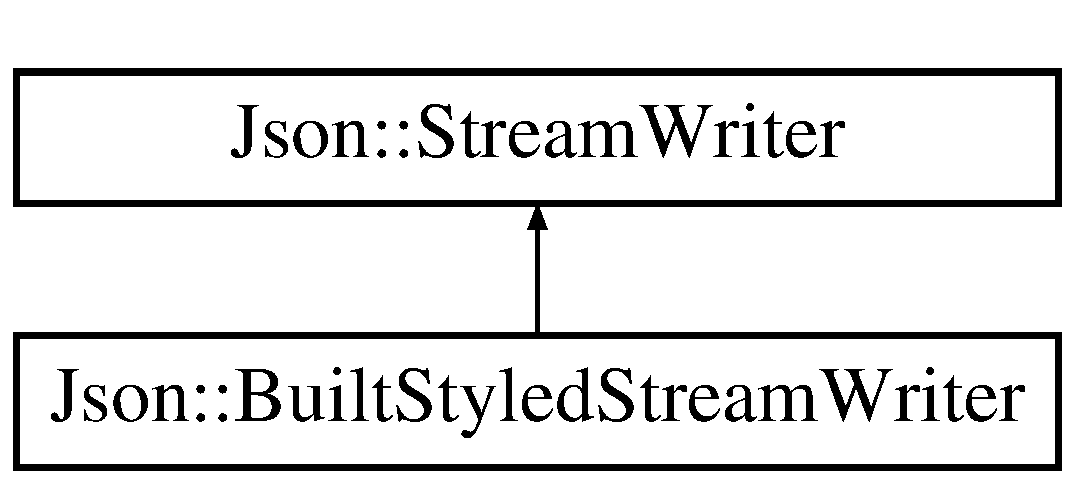
\includegraphics[height=2.000000cm]{structJson_1_1BuiltStyledStreamWriter}
\end{center}
\end{figure}
\subsection*{Public Member Functions}
\begin{DoxyCompactItemize}
\item 
\mbox{\Hypertarget{structJson_1_1BuiltStyledStreamWriter_adf11b7d1ee3c68d096b7c662ee85948e}\label{structJson_1_1BuiltStyledStreamWriter_adf11b7d1ee3c68d096b7c662ee85948e}} 
{\bfseries Built\+Styled\+Stream\+Writer} (J\+S\+O\+N\+C\+P\+P\+\_\+\+S\+T\+R\+I\+NG const \&indentation, \hyperlink{structJson_1_1CommentStyle_a51fc08f3518fd81eba12f340d19a3d0c}{Comment\+Style\+::\+Enum} cs, J\+S\+O\+N\+C\+P\+P\+\_\+\+S\+T\+R\+I\+NG const \&colon\+Symbol, J\+S\+O\+N\+C\+P\+P\+\_\+\+S\+T\+R\+I\+NG const \&null\+Symbol, J\+S\+O\+N\+C\+P\+P\+\_\+\+S\+T\+R\+I\+NG const \&ending\+Line\+Feed\+Symbol, bool use\+Special\+Floats, unsigned int precision)
\item 
int \hyperlink{structJson_1_1BuiltStyledStreamWriter_a823cdb1afabb6b0d5f39bcd5a6a6f747}{write} (\hyperlink{classJson_1_1Value}{Value} const \&root, J\+S\+O\+N\+C\+P\+P\+\_\+\+O\+S\+T\+R\+E\+AM $\ast$sout) J\+S\+O\+N\+C\+P\+P\+\_\+\+O\+V\+E\+R\+R\+I\+DE
\end{DoxyCompactItemize}
\subsection*{Additional Inherited Members}


\subsection{Member Function Documentation}
\mbox{\Hypertarget{structJson_1_1BuiltStyledStreamWriter_a823cdb1afabb6b0d5f39bcd5a6a6f747}\label{structJson_1_1BuiltStyledStreamWriter_a823cdb1afabb6b0d5f39bcd5a6a6f747}} 
\index{Json\+::\+Built\+Styled\+Stream\+Writer@{Json\+::\+Built\+Styled\+Stream\+Writer}!write@{write}}
\index{write@{write}!Json\+::\+Built\+Styled\+Stream\+Writer@{Json\+::\+Built\+Styled\+Stream\+Writer}}
\subsubsection{\texorpdfstring{write()}{write()}}
{\footnotesize\ttfamily int Json\+::\+Built\+Styled\+Stream\+Writer\+::write (\begin{DoxyParamCaption}\item[{\hyperlink{classJson_1_1Value}{Value} const \&}]{root,  }\item[{J\+S\+O\+N\+C\+P\+P\+\_\+\+O\+S\+T\+R\+E\+AM $\ast$}]{sout }\end{DoxyParamCaption})\hspace{0.3cm}{\ttfamily [virtual]}}

Write \hyperlink{classJson_1_1Value}{Value} into document as configured in sub-\/class. Do not take ownership of sout, but maintain a reference during function. \begin{DoxyPrecond}{Precondition}
sout != N\+U\+LL 
\end{DoxyPrecond}
\begin{DoxyReturn}{Returns}
zero on success (For now, we always return zero, so check the stream instead.) 
\end{DoxyReturn}

\begin{DoxyExceptions}{Exceptions}
{\em std\+::exception} & possibly, depending on configuration \\
\hline
\end{DoxyExceptions}


Implements \hyperlink{classJson_1_1StreamWriter_a84278bad0c9a9fc587bc2a97c5bb5993}{Json\+::\+Stream\+Writer}.



The documentation for this struct was generated from the following file\+:\begin{DoxyCompactItemize}
\item 
jsoncpp.\+cpp\end{DoxyCompactItemize}

\hypertarget{unionchar64long16}{}\section{char64long16 Union Reference}
\label{unionchar64long16}\index{char64long16@{char64long16}}
\subsection*{Public Attributes}
\begin{DoxyCompactItemize}
\item 
\mbox{\Hypertarget{unionchar64long16_a7067dbe3b0ff3f11661acb8cd97bcff9}\label{unionchar64long16_a7067dbe3b0ff3f11661acb8cd97bcff9}} 
unsigned char {\bfseries c} \mbox{[}64\mbox{]}
\item 
\mbox{\Hypertarget{unionchar64long16_a4f1edebae3468a551ff2d0cdaecb467d}\label{unionchar64long16_a4f1edebae3468a551ff2d0cdaecb467d}} 
uint32\+\_\+t {\bfseries l} \mbox{[}16\mbox{]}
\end{DoxyCompactItemize}


The documentation for this union was generated from the following file\+:\begin{DoxyCompactItemize}
\item 
mongoose.\+c\end{DoxyCompactItemize}

\hypertarget{classJson_1_1CharReader}{}\section{Json\+:\+:Char\+Reader Class Reference}
\label{classJson_1_1CharReader}\index{Json\+::\+Char\+Reader@{Json\+::\+Char\+Reader}}


{\ttfamily \#include $<$json.\+h$>$}

Inheritance diagram for Json\+:\+:Char\+Reader\+:\begin{figure}[H]
\begin{center}
\leavevmode
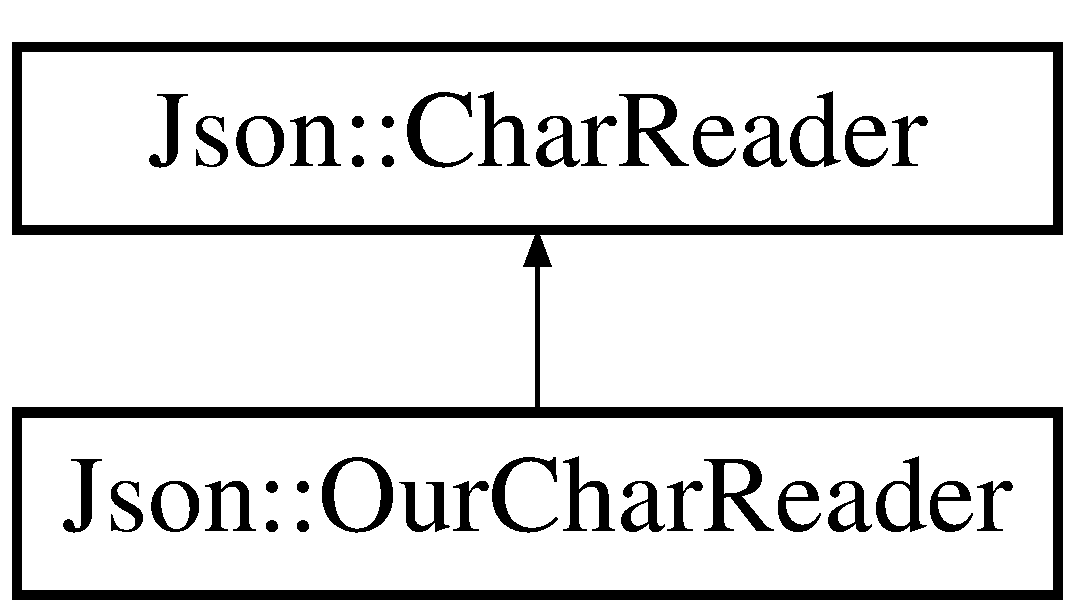
\includegraphics[height=2.000000cm]{classJson_1_1CharReader}
\end{center}
\end{figure}
\subsection*{Classes}
\begin{DoxyCompactItemize}
\item 
class \hyperlink{classJson_1_1CharReader_1_1Factory}{Factory}
\end{DoxyCompactItemize}
\subsection*{Public Member Functions}
\begin{DoxyCompactItemize}
\item 
virtual \hyperlink{classJson_1_1CharReader_acaa7b6ad04fe1cf2ddfca06e66550d7e_acaa7b6ad04fe1cf2ddfca06e66550d7e}{$\sim$\+Char\+Reader} ()
\item 
virtual bool \hyperlink{classJson_1_1CharReader_a7983680d50fd0745f371c43b162e78e1_a7983680d50fd0745f371c43b162e78e1}{parse} (char const $\ast$begin\+Doc, char const $\ast$end\+Doc, \hyperlink{classJson_1_1Value}{Value} $\ast$root, \hyperlink{json_8h_a1e723f95759de062585bc4a8fd3fa4be_a1e723f95759de062585bc4a8fd3fa4be}{J\+S\+O\+N\+C\+P\+P\+\_\+\+S\+T\+R\+I\+NG} $\ast$errs)=0
\begin{DoxyCompactList}\small\item\em Read a \hyperlink{classJson_1_1Value}{Value} from a \href{http://www.json.org}{\tt J\+S\+ON} document. The document must be a U\+T\+F-\/8 encoded string containing the document to read. \end{DoxyCompactList}\end{DoxyCompactItemize}


\subsection{Detailed Description}
Interface for reading J\+S\+ON from a char array. 

\subsection{Constructor \& Destructor Documentation}
\mbox{\Hypertarget{classJson_1_1CharReader_acaa7b6ad04fe1cf2ddfca06e66550d7e_acaa7b6ad04fe1cf2ddfca06e66550d7e}\label{classJson_1_1CharReader_acaa7b6ad04fe1cf2ddfca06e66550d7e_acaa7b6ad04fe1cf2ddfca06e66550d7e}} 
\index{Json\+::\+Char\+Reader@{Json\+::\+Char\+Reader}!````~Char\+Reader@{$\sim$\+Char\+Reader}}
\index{````~Char\+Reader@{$\sim$\+Char\+Reader}!Json\+::\+Char\+Reader@{Json\+::\+Char\+Reader}}
\subsubsection{\texorpdfstring{$\sim$\+Char\+Reader()}{~CharReader()}}
{\footnotesize\ttfamily virtual Json\+::\+Char\+Reader\+::$\sim$\+Char\+Reader (\begin{DoxyParamCaption}{ }\end{DoxyParamCaption})\hspace{0.3cm}{\ttfamily [inline]}, {\ttfamily [virtual]}}



References J\+S\+O\+N\+C\+P\+P\+\_\+\+S\+T\+R\+I\+NG.



\subsection{Member Function Documentation}
\mbox{\Hypertarget{classJson_1_1CharReader_a7983680d50fd0745f371c43b162e78e1_a7983680d50fd0745f371c43b162e78e1}\label{classJson_1_1CharReader_a7983680d50fd0745f371c43b162e78e1_a7983680d50fd0745f371c43b162e78e1}} 
\index{Json\+::\+Char\+Reader@{Json\+::\+Char\+Reader}!parse@{parse}}
\index{parse@{parse}!Json\+::\+Char\+Reader@{Json\+::\+Char\+Reader}}
\subsubsection{\texorpdfstring{parse()}{parse()}}
{\footnotesize\ttfamily virtual bool Json\+::\+Char\+Reader\+::parse (\begin{DoxyParamCaption}\item[{char const $\ast$}]{begin\+Doc,  }\item[{char const $\ast$}]{end\+Doc,  }\item[{\hyperlink{classJson_1_1Value}{Value} $\ast$}]{root,  }\item[{\hyperlink{json_8h_a1e723f95759de062585bc4a8fd3fa4be_a1e723f95759de062585bc4a8fd3fa4be}{J\+S\+O\+N\+C\+P\+P\+\_\+\+S\+T\+R\+I\+NG} $\ast$}]{errs }\end{DoxyParamCaption})\hspace{0.3cm}{\ttfamily [pure virtual]}}



Read a \hyperlink{classJson_1_1Value}{Value} from a \href{http://www.json.org}{\tt J\+S\+ON} document. The document must be a U\+T\+F-\/8 encoded string containing the document to read. 


\begin{DoxyParams}{Parameters}
{\em begin\+Doc} & Pointer on the beginning of the U\+T\+F-\/8 encoded string of the document to read. \\
\hline
{\em end\+Doc} & Pointer on the end of the U\+T\+F-\/8 encoded string of the document to read. Must be $>$= begin\+Doc. \\
\hline
{\em root} & \mbox{[}out\mbox{]} Contains the root value of the document if it was successfully parsed. \\
\hline
{\em errs} & \mbox{[}out\mbox{]} Formatted error messages (if not N\+U\+LL) a user friendly string that lists errors in the parsed document. \\
\hline
\end{DoxyParams}
\begin{DoxyReturn}{Returns}
{\ttfamily true} if the document was successfully parsed, {\ttfamily false} if an error occurred. 
\end{DoxyReturn}


Implemented in \hyperlink{classJson_1_1OurCharReader_a547f08ec5a9951ca69e8bb2e90296c83_a547f08ec5a9951ca69e8bb2e90296c83}{Json\+::\+Our\+Char\+Reader}.



The documentation for this class was generated from the following file\+:\begin{DoxyCompactItemize}
\item 
json/\hyperlink{json_8h}{json.\+h}\end{DoxyCompactItemize}

\hypertarget{classJson_1_1CharReaderBuilder}{}\section{Json\+:\+:Char\+Reader\+Builder Class Reference}
\label{classJson_1_1CharReaderBuilder}\index{Json\+::\+Char\+Reader\+Builder@{Json\+::\+Char\+Reader\+Builder}}


Build a \hyperlink{classJson_1_1CharReader}{Char\+Reader} implementation.  




{\ttfamily \#include $<$json.\+h$>$}

Inheritance diagram for Json\+:\+:Char\+Reader\+Builder\+:\begin{figure}[H]
\begin{center}
\leavevmode
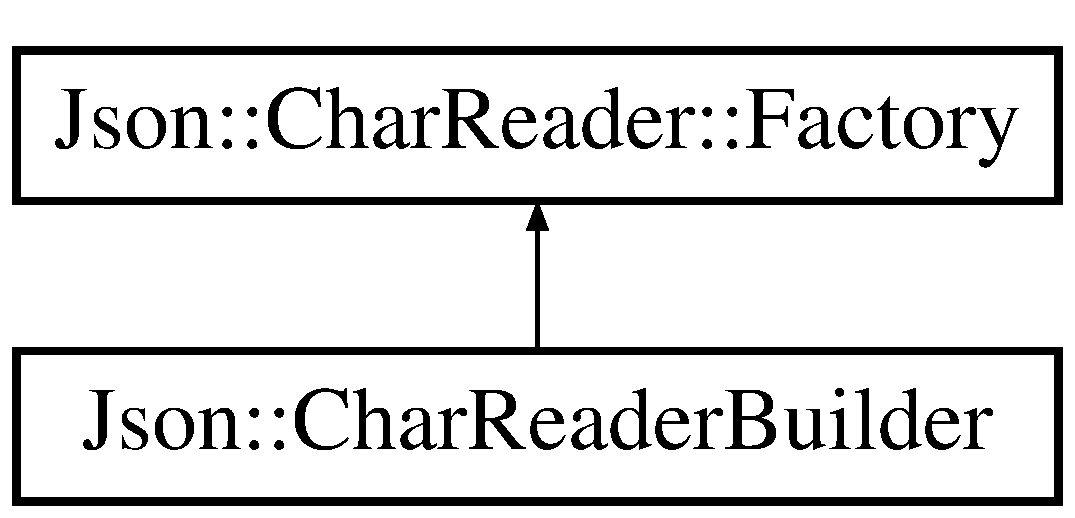
\includegraphics[height=2.000000cm]{classJson_1_1CharReaderBuilder}
\end{center}
\end{figure}
\subsection*{Public Member Functions}
\begin{DoxyCompactItemize}
\item 
\hyperlink{classJson_1_1CharReader}{Char\+Reader} $\ast$ \hyperlink{classJson_1_1CharReaderBuilder_a3a262fcc76c1eb8eebfd4718fb4e9722}{new\+Char\+Reader} () const J\+S\+O\+N\+C\+P\+P\+\_\+\+O\+V\+E\+R\+R\+I\+DE
\begin{DoxyCompactList}\small\item\em Allocate a \hyperlink{classJson_1_1CharReader}{Char\+Reader} via operator new(). \end{DoxyCompactList}\item 
bool \hyperlink{classJson_1_1CharReaderBuilder_af890b5cb70e9b372e41de5c9e6535d21}{validate} (\hyperlink{classJson_1_1Value}{Json\+::\+Value} $\ast$invalid) const
\item 
\hyperlink{classJson_1_1Value}{Value} \& \hyperlink{classJson_1_1CharReaderBuilder_a84b35ef443340c06c0aa7b47851d8d86}{operator\mbox{[}$\,$\mbox{]}} (J\+S\+O\+N\+C\+P\+P\+\_\+\+S\+T\+R\+I\+NG key)
\end{DoxyCompactItemize}
\subsection*{Static Public Member Functions}
\begin{DoxyCompactItemize}
\item 
static void \hyperlink{classJson_1_1CharReaderBuilder_a03ff031e06aabff989ab4addc87294ab}{set\+Defaults} (\hyperlink{classJson_1_1Value}{Json\+::\+Value} $\ast$settings)
\item 
static void \hyperlink{classJson_1_1CharReaderBuilder_a9c19e3c5475f9072d527810d4bf56749}{strict\+Mode} (\hyperlink{classJson_1_1Value}{Json\+::\+Value} $\ast$settings)
\end{DoxyCompactItemize}
\subsection*{Public Attributes}
\begin{DoxyCompactItemize}
\item 
\hyperlink{classJson_1_1Value}{Json\+::\+Value} \hyperlink{classJson_1_1CharReaderBuilder_ac69b7911ad64c171c51ebaf2ea26d958}{settings\+\_\+}
\end{DoxyCompactItemize}


\subsection{Detailed Description}
Build a \hyperlink{classJson_1_1CharReader}{Char\+Reader} implementation. 

Usage\+: 
\begin{DoxyCode}
\textcolor{keyword}{using namespace }\hyperlink{namespaceJson}{Json};
\hyperlink{classJson_1_1CharReaderBuilder}{CharReaderBuilder} builder;
builder[\textcolor{stringliteral}{"collectComments"}] = \textcolor{keyword}{false};
\hyperlink{classJson_1_1Value}{Value} value;
JSONCPP\_STRING errs;
\textcolor{keywordtype}{bool} ok = \hyperlink{namespaceJson_aab0cf1ecf81d1aeca12be2a416a84352}{parseFromStream}(builder, std::cin, &value, &errs);
\end{DoxyCode}
 

\subsection{Member Function Documentation}
\mbox{\Hypertarget{classJson_1_1CharReaderBuilder_a3a262fcc76c1eb8eebfd4718fb4e9722}\label{classJson_1_1CharReaderBuilder_a3a262fcc76c1eb8eebfd4718fb4e9722}} 
\index{Json\+::\+Char\+Reader\+Builder@{Json\+::\+Char\+Reader\+Builder}!new\+Char\+Reader@{new\+Char\+Reader}}
\index{new\+Char\+Reader@{new\+Char\+Reader}!Json\+::\+Char\+Reader\+Builder@{Json\+::\+Char\+Reader\+Builder}}
\subsubsection{\texorpdfstring{new\+Char\+Reader()}{newCharReader()}}
{\footnotesize\ttfamily \hyperlink{classJson_1_1CharReader}{Char\+Reader} $\ast$ Json\+::\+Char\+Reader\+Builder\+::new\+Char\+Reader (\begin{DoxyParamCaption}{ }\end{DoxyParamCaption}) const\hspace{0.3cm}{\ttfamily [virtual]}}



Allocate a \hyperlink{classJson_1_1CharReader}{Char\+Reader} via operator new(). 


\begin{DoxyExceptions}{Exceptions}
{\em std\+::exception} & if something goes wrong (e.\+g. invalid settings) \\
\hline
\end{DoxyExceptions}


Implements \hyperlink{classJson_1_1CharReader_1_1Factory_a4c5862a1ffd432372dbe65cf59de98c4}{Json\+::\+Char\+Reader\+::\+Factory}.

\mbox{\Hypertarget{classJson_1_1CharReaderBuilder_a84b35ef443340c06c0aa7b47851d8d86}\label{classJson_1_1CharReaderBuilder_a84b35ef443340c06c0aa7b47851d8d86}} 
\index{Json\+::\+Char\+Reader\+Builder@{Json\+::\+Char\+Reader\+Builder}!operator\mbox{[}\mbox{]}@{operator[]}}
\index{operator\mbox{[}\mbox{]}@{operator[]}!Json\+::\+Char\+Reader\+Builder@{Json\+::\+Char\+Reader\+Builder}}
\subsubsection{\texorpdfstring{operator[]()}{operator[]()}}
{\footnotesize\ttfamily \hyperlink{classJson_1_1Value}{Value} \& Json\+::\+Char\+Reader\+Builder\+::operator\mbox{[}$\,$\mbox{]} (\begin{DoxyParamCaption}\item[{J\+S\+O\+N\+C\+P\+P\+\_\+\+S\+T\+R\+I\+NG}]{key }\end{DoxyParamCaption})}

A simple way to update a specific setting. \mbox{\Hypertarget{classJson_1_1CharReaderBuilder_a03ff031e06aabff989ab4addc87294ab}\label{classJson_1_1CharReaderBuilder_a03ff031e06aabff989ab4addc87294ab}} 
\index{Json\+::\+Char\+Reader\+Builder@{Json\+::\+Char\+Reader\+Builder}!set\+Defaults@{set\+Defaults}}
\index{set\+Defaults@{set\+Defaults}!Json\+::\+Char\+Reader\+Builder@{Json\+::\+Char\+Reader\+Builder}}
\subsubsection{\texorpdfstring{set\+Defaults()}{setDefaults()}}
{\footnotesize\ttfamily void Json\+::\+Char\+Reader\+Builder\+::set\+Defaults (\begin{DoxyParamCaption}\item[{\hyperlink{classJson_1_1Value}{Json\+::\+Value} $\ast$}]{settings }\end{DoxyParamCaption})\hspace{0.3cm}{\ttfamily [static]}}

Called by ctor, but you can use this to reset settings\+\_\+. \begin{DoxyPrecond}{Precondition}
\textquotesingle{}settings\textquotesingle{} != N\+U\+LL (but Json\+::null is fine) 
\end{DoxyPrecond}
\begin{DoxyRemark}{Remarks}
Defaults\+: 
\begin{DoxyCodeInclude}
\end{DoxyCodeInclude}

\end{DoxyRemark}
\mbox{[}Char\+Reader\+Builder\+Defaults\mbox{]}

\mbox{[}Char\+Reader\+Builder\+Defaults\mbox{]} \mbox{\Hypertarget{classJson_1_1CharReaderBuilder_a9c19e3c5475f9072d527810d4bf56749}\label{classJson_1_1CharReaderBuilder_a9c19e3c5475f9072d527810d4bf56749}} 
\index{Json\+::\+Char\+Reader\+Builder@{Json\+::\+Char\+Reader\+Builder}!strict\+Mode@{strict\+Mode}}
\index{strict\+Mode@{strict\+Mode}!Json\+::\+Char\+Reader\+Builder@{Json\+::\+Char\+Reader\+Builder}}
\subsubsection{\texorpdfstring{strict\+Mode()}{strictMode()}}
{\footnotesize\ttfamily void Json\+::\+Char\+Reader\+Builder\+::strict\+Mode (\begin{DoxyParamCaption}\item[{\hyperlink{classJson_1_1Value}{Json\+::\+Value} $\ast$}]{settings }\end{DoxyParamCaption})\hspace{0.3cm}{\ttfamily [static]}}

Same as old \hyperlink{classJson_1_1Features_ae23176c14b2e79e81fb61fb1a8ab58ee}{Features\+::strict\+Mode()}. \begin{DoxyPrecond}{Precondition}
\textquotesingle{}settings\textquotesingle{} != N\+U\+LL (but Json\+::null is fine) 
\end{DoxyPrecond}
\begin{DoxyRemark}{Remarks}
Defaults\+: 
\begin{DoxyCodeInclude}
\end{DoxyCodeInclude}

\end{DoxyRemark}
\mbox{[}Char\+Reader\+Builder\+Strict\+Mode\mbox{]}

\mbox{[}Char\+Reader\+Builder\+Strict\+Mode\mbox{]} \mbox{\Hypertarget{classJson_1_1CharReaderBuilder_af890b5cb70e9b372e41de5c9e6535d21}\label{classJson_1_1CharReaderBuilder_af890b5cb70e9b372e41de5c9e6535d21}} 
\index{Json\+::\+Char\+Reader\+Builder@{Json\+::\+Char\+Reader\+Builder}!validate@{validate}}
\index{validate@{validate}!Json\+::\+Char\+Reader\+Builder@{Json\+::\+Char\+Reader\+Builder}}
\subsubsection{\texorpdfstring{validate()}{validate()}}
{\footnotesize\ttfamily bool Json\+::\+Char\+Reader\+Builder\+::validate (\begin{DoxyParamCaption}\item[{\hyperlink{classJson_1_1Value}{Json\+::\+Value} $\ast$}]{invalid }\end{DoxyParamCaption}) const}

\begin{DoxyReturn}{Returns}
true if \textquotesingle{}settings\textquotesingle{} are legal and consistent; otherwise, indicate bad settings via \textquotesingle{}invalid\textquotesingle{}. 
\end{DoxyReturn}


\subsection{Member Data Documentation}
\mbox{\Hypertarget{classJson_1_1CharReaderBuilder_ac69b7911ad64c171c51ebaf2ea26d958}\label{classJson_1_1CharReaderBuilder_ac69b7911ad64c171c51ebaf2ea26d958}} 
\index{Json\+::\+Char\+Reader\+Builder@{Json\+::\+Char\+Reader\+Builder}!settings\+\_\+@{settings\+\_\+}}
\index{settings\+\_\+@{settings\+\_\+}!Json\+::\+Char\+Reader\+Builder@{Json\+::\+Char\+Reader\+Builder}}
\subsubsection{\texorpdfstring{settings\+\_\+}{settings\_}}
{\footnotesize\ttfamily \hyperlink{classJson_1_1Value}{Json\+::\+Value} Json\+::\+Char\+Reader\+Builder\+::settings\+\_\+}

Configuration of this builder. These are case-\/sensitive. Available settings (case-\/sensitive)\+:
\begin{DoxyItemize}
\item {\ttfamily \char`\"{}collect\+Comments\char`\"{}\+: false or true}
\begin{DoxyItemize}
\item true to collect comment and allow writing them back during serialization, false to discard comments. This parameter is ignored if allow\+Comments is false.
\end{DoxyItemize}
\item {\ttfamily \char`\"{}allow\+Comments\char`\"{}\+: false or true}
\begin{DoxyItemize}
\item true if comments are allowed.
\end{DoxyItemize}
\item {\ttfamily \char`\"{}strict\+Root\char`\"{}\+: false or true}
\begin{DoxyItemize}
\item true if root must be either an array or an object value
\end{DoxyItemize}
\item {\ttfamily \char`\"{}allow\+Dropped\+Null\+Placeholders\char`\"{}\+: false or true}
\begin{DoxyItemize}
\item true if dropped null placeholders are allowed. (See \hyperlink{classJson_1_1StreamWriterBuilder}{Stream\+Writer\+Builder}.)
\end{DoxyItemize}
\item {\ttfamily \char`\"{}allow\+Numeric\+Keys\char`\"{}\+: false or true}
\begin{DoxyItemize}
\item true if numeric object keys are allowed.
\end{DoxyItemize}
\item {\ttfamily \char`\"{}allow\+Single\+Quotes\char`\"{}\+: false or true}
\begin{DoxyItemize}
\item true if \textquotesingle{}\textquotesingle{} are allowed for strings (both keys and values)
\end{DoxyItemize}
\item {\ttfamily \char`\"{}stack\+Limit\char`\"{}\+: integer}
\begin{DoxyItemize}
\item Exceeding stack\+Limit (recursive depth of {\ttfamily read\+Value()}) will cause an exception.
\item This is a security issue (seg-\/faults caused by deeply nested J\+S\+ON), so the default is low.
\end{DoxyItemize}
\item {\ttfamily \char`\"{}fail\+If\+Extra\char`\"{}\+: false or true}
\begin{DoxyItemize}
\item If true, {\ttfamily parse()} returns false when extra non-\/whitespace trails the J\+S\+ON value in the input string.
\end{DoxyItemize}
\item {\ttfamily \char`\"{}reject\+Dup\+Keys\char`\"{}\+: false or true}
\begin{DoxyItemize}
\item If true, {\ttfamily parse()} returns false when a key is duplicated within an object.
\end{DoxyItemize}
\item {\ttfamily \char`\"{}allow\+Special\+Floats\char`\"{}\+: false or true}
\begin{DoxyItemize}
\item If true, special float values (Na\+Ns and infinities) are allowed and their values are lossfree restorable.
\end{DoxyItemize}
\end{DoxyItemize}

You can examine \textquotesingle{}settings\+\_\+` yourself to see the defaults. You can also write and read them just like any J\+S\+ON \hyperlink{classJson_1_1Value}{Value}. \begin{DoxySeeAlso}{See also}
\hyperlink{classJson_1_1CharReaderBuilder_a03ff031e06aabff989ab4addc87294ab}{set\+Defaults()} 
\end{DoxySeeAlso}


The documentation for this class was generated from the following files\+:\begin{DoxyCompactItemize}
\item 
json/json.\+h\item 
jsoncpp.\+cpp\end{DoxyCompactItemize}

\hypertarget{classTBT_1_1Client}{}\section{T\+BT\+:\+:Client Class Reference}
\label{classTBT_1_1Client}\index{T\+B\+T\+::\+Client@{T\+B\+T\+::\+Client}}
Inheritance diagram for T\+BT\+:\+:Client\+:\begin{figure}[H]
\begin{center}
\leavevmode
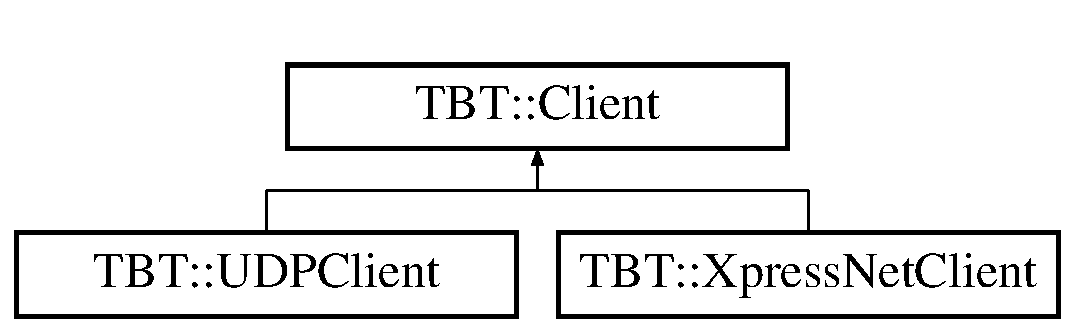
\includegraphics[height=2.000000cm]{classTBT_1_1Client}
\end{center}
\end{figure}
\subsection*{Public Member Functions}
\begin{DoxyCompactItemize}
\item 
\mbox{\Hypertarget{classTBT_1_1Client_a6220a6ee1345c62986aea535e2ae202c}\label{classTBT_1_1Client_a6220a6ee1345c62986aea535e2ae202c}} 
{\bfseries Client} (\hyperlink{classTBT_1_1ClientInterface}{Client\+Interface} $\ast$p\+Interface)
\item 
\mbox{\Hypertarget{classTBT_1_1Client_a37d9a9919aa90879dbf46cf95e519259}\label{classTBT_1_1Client_a37d9a9919aa90879dbf46cf95e519259}} 
\hyperlink{classTBT_1_1ClientInterface}{Client\+Interface} $\ast$ {\bfseries get\+Interface} (void)
\item 
\mbox{\Hypertarget{classTBT_1_1Client_ad64588b494ec98154ea261ed4f3b3643}\label{classTBT_1_1Client_ad64588b494ec98154ea261ed4f3b3643}} 
virtual void {\bfseries broadcast\+Power\+State\+Change} (bool new\+State)=0
\item 
\mbox{\Hypertarget{classTBT_1_1Client_aeb3b63a37edc6b95872df54a57c27a71}\label{classTBT_1_1Client_aeb3b63a37edc6b95872df54a57c27a71}} 
virtual void {\bfseries broadcast\+Loc\+Info\+Changed} (\hyperlink{classTBT_1_1LocDecoder}{Loc\+Decoder} $\ast$p\+Loc)=0
\item 
\mbox{\Hypertarget{classTBT_1_1Client_a59459df809a663bcbbb6d31fbfa09402}\label{classTBT_1_1Client_a59459df809a663bcbbb6d31fbfa09402}} 
virtual void {\bfseries broadcast\+Emergency\+Stop} (void)=0
\end{DoxyCompactItemize}
\subsection*{Protected Attributes}
\begin{DoxyCompactItemize}
\item 
\mbox{\Hypertarget{classTBT_1_1Client_a0b3e41f73f6381600c8ddac129b740f6}\label{classTBT_1_1Client_a0b3e41f73f6381600c8ddac129b740f6}} 
\hyperlink{classTBT_1_1ClientInterface}{Client\+Interface} $\ast$ {\bfseries m\+\_\+p\+Interface}
\end{DoxyCompactItemize}


The documentation for this class was generated from the following files\+:\begin{DoxyCompactItemize}
\item 
Client.\+h\item 
Client.\+cpp\end{DoxyCompactItemize}

\hypertarget{classTBT_1_1ClientInterface}{}\section{T\+BT\+:\+:Client\+Interface Class Reference}
\label{classTBT_1_1ClientInterface}\index{T\+B\+T\+::\+Client\+Interface@{T\+B\+T\+::\+Client\+Interface}}


{\ttfamily \#include $<$Client\+Interface.\+h$>$}

Inheritance diagram for T\+BT\+:\+:Client\+Interface\+:\begin{figure}[H]
\begin{center}
\leavevmode
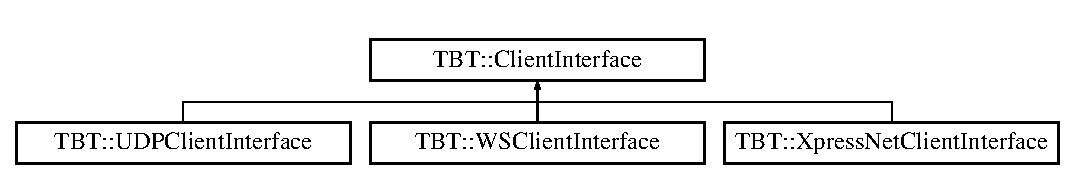
\includegraphics[height=1.975309cm]{classTBT_1_1ClientInterface}
\end{center}
\end{figure}
\subsection*{Public Member Functions}
\begin{DoxyCompactItemize}
\item 
\hyperlink{classTBT_1_1ClientInterface_a77cd35b080e78932f2371ea0f897964b_a77cd35b080e78932f2371ea0f897964b}{Client\+Interface} (\hyperlink{classTBT_1_1Manager}{Manager} $\ast$p\+Manager)
\item 
virtual \hyperlink{classTBT_1_1ClientInterface_aa42abb5947fa0af75eed777325cbff27_aa42abb5947fa0af75eed777325cbff27}{$\sim$\+Client\+Interface} ()
\item 
\hyperlink{classTBT_1_1Manager}{Manager} $\ast$ \hyperlink{classTBT_1_1ClientInterface_a26e144856b1253744b20c5638065acf7_a26e144856b1253744b20c5638065acf7}{get\+Manager} (void)
\item 
virtual void \hyperlink{classTBT_1_1ClientInterface_a7888a3446fb416fad75e5e008a85ca0c_a7888a3446fb416fad75e5e008a85ca0c}{broadcast\+Power\+State\+Change} (bool new\+State)=0
\item 
virtual void \hyperlink{classTBT_1_1ClientInterface_aaede3709fa0dcb23743f43d9c1a5ab04_aaede3709fa0dcb23743f43d9c1a5ab04}{broadcast\+Loc\+Info\+Change} (\hyperlink{classTBT_1_1LocDecoder}{Loc\+Decoder} $\ast$p\+Loc)=0
\item 
virtual void \hyperlink{classTBT_1_1ClientInterface_a8d19220baccb47a7c9f45d0288bebcb8_a8d19220baccb47a7c9f45d0288bebcb8}{broadcast\+Emergency\+Stop} (void)=0
\end{DoxyCompactItemize}
\subsection*{Protected Attributes}
\begin{DoxyCompactItemize}
\item 
\hyperlink{classTBT_1_1Manager}{Manager} $\ast$ \hyperlink{classTBT_1_1ClientInterface_a1d6558ab5cd2ebcc135e5fc37a1844ba_a1d6558ab5cd2ebcc135e5fc37a1844ba}{m\+\_\+p\+Manager}
\end{DoxyCompactItemize}


\subsection{Constructor \& Destructor Documentation}
\mbox{\Hypertarget{classTBT_1_1ClientInterface_a77cd35b080e78932f2371ea0f897964b_a77cd35b080e78932f2371ea0f897964b}\label{classTBT_1_1ClientInterface_a77cd35b080e78932f2371ea0f897964b_a77cd35b080e78932f2371ea0f897964b}} 
\index{T\+B\+T\+::\+Client\+Interface@{T\+B\+T\+::\+Client\+Interface}!Client\+Interface@{Client\+Interface}}
\index{Client\+Interface@{Client\+Interface}!T\+B\+T\+::\+Client\+Interface@{T\+B\+T\+::\+Client\+Interface}}
\subsubsection{\texorpdfstring{Client\+Interface()}{ClientInterface()}}
{\footnotesize\ttfamily T\+B\+T\+::\+Client\+Interface\+::\+Client\+Interface (\begin{DoxyParamCaption}\item[{\hyperlink{classTBT_1_1Manager}{Manager} $\ast$}]{p\+Manager }\end{DoxyParamCaption})}

\mbox{\Hypertarget{classTBT_1_1ClientInterface_aa42abb5947fa0af75eed777325cbff27_aa42abb5947fa0af75eed777325cbff27}\label{classTBT_1_1ClientInterface_aa42abb5947fa0af75eed777325cbff27_aa42abb5947fa0af75eed777325cbff27}} 
\index{T\+B\+T\+::\+Client\+Interface@{T\+B\+T\+::\+Client\+Interface}!````~Client\+Interface@{$\sim$\+Client\+Interface}}
\index{````~Client\+Interface@{$\sim$\+Client\+Interface}!T\+B\+T\+::\+Client\+Interface@{T\+B\+T\+::\+Client\+Interface}}
\subsubsection{\texorpdfstring{$\sim$\+Client\+Interface()}{~ClientInterface()}}
{\footnotesize\ttfamily T\+B\+T\+::\+Client\+Interface\+::$\sim$\+Client\+Interface (\begin{DoxyParamCaption}{ }\end{DoxyParamCaption})\hspace{0.3cm}{\ttfamily [virtual]}}



\subsection{Member Function Documentation}
\mbox{\Hypertarget{classTBT_1_1ClientInterface_a8d19220baccb47a7c9f45d0288bebcb8_a8d19220baccb47a7c9f45d0288bebcb8}\label{classTBT_1_1ClientInterface_a8d19220baccb47a7c9f45d0288bebcb8_a8d19220baccb47a7c9f45d0288bebcb8}} 
\index{T\+B\+T\+::\+Client\+Interface@{T\+B\+T\+::\+Client\+Interface}!broadcast\+Emergency\+Stop@{broadcast\+Emergency\+Stop}}
\index{broadcast\+Emergency\+Stop@{broadcast\+Emergency\+Stop}!T\+B\+T\+::\+Client\+Interface@{T\+B\+T\+::\+Client\+Interface}}
\subsubsection{\texorpdfstring{broadcast\+Emergency\+Stop()}{broadcastEmergencyStop()}}
{\footnotesize\ttfamily virtual void T\+B\+T\+::\+Client\+Interface\+::broadcast\+Emergency\+Stop (\begin{DoxyParamCaption}\item[{void}]{ }\end{DoxyParamCaption})\hspace{0.3cm}{\ttfamily [pure virtual]}}



Implemented in \hyperlink{classTBT_1_1UDPClientInterface_a33a0c51d141a457cda9dacc4d82d5304_a33a0c51d141a457cda9dacc4d82d5304}{T\+B\+T\+::\+U\+D\+P\+Client\+Interface}, \hyperlink{classTBT_1_1WSClientInterface_a2ad439e557711c57c8a978e3b6efcb62_a2ad439e557711c57c8a978e3b6efcb62}{T\+B\+T\+::\+W\+S\+Client\+Interface}, and \hyperlink{classTBT_1_1XpressNetClientInterface_a143641241f4830f22ec5beb78036ce4c_a143641241f4830f22ec5beb78036ce4c}{T\+B\+T\+::\+Xpress\+Net\+Client\+Interface}.



Referenced by get\+Manager().

\mbox{\Hypertarget{classTBT_1_1ClientInterface_aaede3709fa0dcb23743f43d9c1a5ab04_aaede3709fa0dcb23743f43d9c1a5ab04}\label{classTBT_1_1ClientInterface_aaede3709fa0dcb23743f43d9c1a5ab04_aaede3709fa0dcb23743f43d9c1a5ab04}} 
\index{T\+B\+T\+::\+Client\+Interface@{T\+B\+T\+::\+Client\+Interface}!broadcast\+Loc\+Info\+Change@{broadcast\+Loc\+Info\+Change}}
\index{broadcast\+Loc\+Info\+Change@{broadcast\+Loc\+Info\+Change}!T\+B\+T\+::\+Client\+Interface@{T\+B\+T\+::\+Client\+Interface}}
\subsubsection{\texorpdfstring{broadcast\+Loc\+Info\+Change()}{broadcastLocInfoChange()}}
{\footnotesize\ttfamily virtual void T\+B\+T\+::\+Client\+Interface\+::broadcast\+Loc\+Info\+Change (\begin{DoxyParamCaption}\item[{\hyperlink{classTBT_1_1LocDecoder}{Loc\+Decoder} $\ast$}]{p\+Loc }\end{DoxyParamCaption})\hspace{0.3cm}{\ttfamily [pure virtual]}}



Implemented in \hyperlink{classTBT_1_1UDPClientInterface_af4e63115b3156b151d4dfd50342b36e7_af4e63115b3156b151d4dfd50342b36e7}{T\+B\+T\+::\+U\+D\+P\+Client\+Interface}, \hyperlink{classTBT_1_1WSClientInterface_a39806206461815c06c517b66d122b4db_a39806206461815c06c517b66d122b4db}{T\+B\+T\+::\+W\+S\+Client\+Interface}, and \hyperlink{classTBT_1_1XpressNetClientInterface_a8e64404cb84913c2d9290d2afb882b39_a8e64404cb84913c2d9290d2afb882b39}{T\+B\+T\+::\+Xpress\+Net\+Client\+Interface}.



Referenced by get\+Manager().

\mbox{\Hypertarget{classTBT_1_1ClientInterface_a7888a3446fb416fad75e5e008a85ca0c_a7888a3446fb416fad75e5e008a85ca0c}\label{classTBT_1_1ClientInterface_a7888a3446fb416fad75e5e008a85ca0c_a7888a3446fb416fad75e5e008a85ca0c}} 
\index{T\+B\+T\+::\+Client\+Interface@{T\+B\+T\+::\+Client\+Interface}!broadcast\+Power\+State\+Change@{broadcast\+Power\+State\+Change}}
\index{broadcast\+Power\+State\+Change@{broadcast\+Power\+State\+Change}!T\+B\+T\+::\+Client\+Interface@{T\+B\+T\+::\+Client\+Interface}}
\subsubsection{\texorpdfstring{broadcast\+Power\+State\+Change()}{broadcastPowerStateChange()}}
{\footnotesize\ttfamily virtual void T\+B\+T\+::\+Client\+Interface\+::broadcast\+Power\+State\+Change (\begin{DoxyParamCaption}\item[{bool}]{new\+State }\end{DoxyParamCaption})\hspace{0.3cm}{\ttfamily [pure virtual]}}



Implemented in \hyperlink{classTBT_1_1UDPClientInterface_a60ddc3657a12b4e6c7ef7db0a31c9e3c_a60ddc3657a12b4e6c7ef7db0a31c9e3c}{T\+B\+T\+::\+U\+D\+P\+Client\+Interface}, \hyperlink{classTBT_1_1WSClientInterface_ad1c7f413c63f04b04d6e20f5d154d1fd_ad1c7f413c63f04b04d6e20f5d154d1fd}{T\+B\+T\+::\+W\+S\+Client\+Interface}, and \hyperlink{classTBT_1_1XpressNetClientInterface_a338da1925ec68f197e87625c7497f472_a338da1925ec68f197e87625c7497f472}{T\+B\+T\+::\+Xpress\+Net\+Client\+Interface}.



Referenced by get\+Manager().

\mbox{\Hypertarget{classTBT_1_1ClientInterface_a26e144856b1253744b20c5638065acf7_a26e144856b1253744b20c5638065acf7}\label{classTBT_1_1ClientInterface_a26e144856b1253744b20c5638065acf7_a26e144856b1253744b20c5638065acf7}} 
\index{T\+B\+T\+::\+Client\+Interface@{T\+B\+T\+::\+Client\+Interface}!get\+Manager@{get\+Manager}}
\index{get\+Manager@{get\+Manager}!T\+B\+T\+::\+Client\+Interface@{T\+B\+T\+::\+Client\+Interface}}
\subsubsection{\texorpdfstring{get\+Manager()}{getManager()}}
{\footnotesize\ttfamily \hyperlink{classTBT_1_1Manager}{Manager}$\ast$ T\+B\+T\+::\+Client\+Interface\+::get\+Manager (\begin{DoxyParamCaption}\item[{void}]{ }\end{DoxyParamCaption})\hspace{0.3cm}{\ttfamily [inline]}}



References broadcast\+Emergency\+Stop(), broadcast\+Loc\+Info\+Change(), broadcast\+Power\+State\+Change(), and m\+\_\+p\+Manager.



Referenced by T\+B\+T\+::\+Xpress\+Net\+Client\+Interface\+::thread\+Func(), and T\+B\+T\+::\+U\+D\+P\+Client\+Interface\+::thread\+Func().



\subsection{Member Data Documentation}
\mbox{\Hypertarget{classTBT_1_1ClientInterface_a1d6558ab5cd2ebcc135e5fc37a1844ba_a1d6558ab5cd2ebcc135e5fc37a1844ba}\label{classTBT_1_1ClientInterface_a1d6558ab5cd2ebcc135e5fc37a1844ba_a1d6558ab5cd2ebcc135e5fc37a1844ba}} 
\index{T\+B\+T\+::\+Client\+Interface@{T\+B\+T\+::\+Client\+Interface}!m\+\_\+p\+Manager@{m\+\_\+p\+Manager}}
\index{m\+\_\+p\+Manager@{m\+\_\+p\+Manager}!T\+B\+T\+::\+Client\+Interface@{T\+B\+T\+::\+Client\+Interface}}
\subsubsection{\texorpdfstring{m\+\_\+p\+Manager}{m\_pManager}}
{\footnotesize\ttfamily \hyperlink{classTBT_1_1Manager}{Manager}$\ast$ T\+B\+T\+::\+Client\+Interface\+::m\+\_\+p\+Manager\hspace{0.3cm}{\ttfamily [protected]}}



Referenced by get\+Manager().



The documentation for this class was generated from the following files\+:\begin{DoxyCompactItemize}
\item 
\hyperlink{ClientInterface_8h}{Client\+Interface.\+h}\item 
\hyperlink{ClientInterface_8cpp}{Client\+Interface.\+cpp}\end{DoxyCompactItemize}

\hypertarget{structJson_1_1CommentStyle}{}\section{Json\+:\+:Comment\+Style Struct Reference}
\label{structJson_1_1CommentStyle}\index{Json\+::\+Comment\+Style@{Json\+::\+Comment\+Style}}


Scoped enums are not available until C++11.  


\subsection*{Public Types}
\begin{DoxyCompactItemize}
\item 
enum \hyperlink{structJson_1_1CommentStyle_a51fc08f3518fd81eba12f340d19a3d0c}{Enum} \{ \hyperlink{structJson_1_1CommentStyle_a51fc08f3518fd81eba12f340d19a3d0cac8b32a8bae63414c8647d4919da8d437}{None}, 
\hyperlink{structJson_1_1CommentStyle_a51fc08f3518fd81eba12f340d19a3d0cac65238f050773c107690a456e9c05c98}{Most}, 
\hyperlink{structJson_1_1CommentStyle_a51fc08f3518fd81eba12f340d19a3d0ca32302c0b97190c1808b3e38f367fef01}{All}
 \}\begin{DoxyCompactList}\small\item\em Decide whether to write comments. \end{DoxyCompactList}
\end{DoxyCompactItemize}


\subsection{Detailed Description}
Scoped enums are not available until C++11. 

\subsection{Member Enumeration Documentation}
\mbox{\Hypertarget{structJson_1_1CommentStyle_a51fc08f3518fd81eba12f340d19a3d0c}\label{structJson_1_1CommentStyle_a51fc08f3518fd81eba12f340d19a3d0c}} 
\index{Json\+::\+Comment\+Style@{Json\+::\+Comment\+Style}!Enum@{Enum}}
\index{Enum@{Enum}!Json\+::\+Comment\+Style@{Json\+::\+Comment\+Style}}
\subsubsection{\texorpdfstring{Enum}{Enum}}
{\footnotesize\ttfamily enum \hyperlink{structJson_1_1CommentStyle_a51fc08f3518fd81eba12f340d19a3d0c}{Json\+::\+Comment\+Style\+::\+Enum}}



Decide whether to write comments. 

\begin{DoxyEnumFields}{Enumerator}
\raisebox{\heightof{T}}[0pt][0pt]{\index{None@{None}!Json\+::\+Comment\+Style@{Json\+::\+Comment\+Style}}\index{Json\+::\+Comment\+Style@{Json\+::\+Comment\+Style}!None@{None}}}\mbox{\Hypertarget{structJson_1_1CommentStyle_a51fc08f3518fd81eba12f340d19a3d0cac8b32a8bae63414c8647d4919da8d437}\label{structJson_1_1CommentStyle_a51fc08f3518fd81eba12f340d19a3d0cac8b32a8bae63414c8647d4919da8d437}} 
None&Drop all comments. \\
\hline

\raisebox{\heightof{T}}[0pt][0pt]{\index{Most@{Most}!Json\+::\+Comment\+Style@{Json\+::\+Comment\+Style}}\index{Json\+::\+Comment\+Style@{Json\+::\+Comment\+Style}!Most@{Most}}}\mbox{\Hypertarget{structJson_1_1CommentStyle_a51fc08f3518fd81eba12f340d19a3d0cac65238f050773c107690a456e9c05c98}\label{structJson_1_1CommentStyle_a51fc08f3518fd81eba12f340d19a3d0cac65238f050773c107690a456e9c05c98}} 
Most&Recover odd behavior of previous versions (not implemented yet). \\
\hline

\raisebox{\heightof{T}}[0pt][0pt]{\index{All@{All}!Json\+::\+Comment\+Style@{Json\+::\+Comment\+Style}}\index{Json\+::\+Comment\+Style@{Json\+::\+Comment\+Style}!All@{All}}}\mbox{\Hypertarget{structJson_1_1CommentStyle_a51fc08f3518fd81eba12f340d19a3d0ca32302c0b97190c1808b3e38f367fef01}\label{structJson_1_1CommentStyle_a51fc08f3518fd81eba12f340d19a3d0ca32302c0b97190c1808b3e38f367fef01}} 
All&Keep all comments. \\
\hline

\end{DoxyEnumFields}


The documentation for this struct was generated from the following file\+:\begin{DoxyCompactItemize}
\item 
jsoncpp.\+cpp\end{DoxyCompactItemize}

\hypertarget{structcs__base64__ctx}{}\section{cs\+\_\+base64\+\_\+ctx Struct Reference}
\label{structcs__base64__ctx}\index{cs\+\_\+base64\+\_\+ctx@{cs\+\_\+base64\+\_\+ctx}}
\subsection*{Public Attributes}
\begin{DoxyCompactItemize}
\item 
\mbox{\Hypertarget{structcs__base64__ctx_a59b8384fbdd1681555a9dd18ed6585ae}\label{structcs__base64__ctx_a59b8384fbdd1681555a9dd18ed6585ae}} 
cs\+\_\+base64\+\_\+putc\+\_\+t {\bfseries b64\+\_\+putc}
\item 
\mbox{\Hypertarget{structcs__base64__ctx_a209b5eff716d6a1850cca128ed5b070e}\label{structcs__base64__ctx_a209b5eff716d6a1850cca128ed5b070e}} 
unsigned char {\bfseries chunk} \mbox{[}3\mbox{]}
\item 
\mbox{\Hypertarget{structcs__base64__ctx_a5753baf57fe83161369e2270d57e4a9e}\label{structcs__base64__ctx_a5753baf57fe83161369e2270d57e4a9e}} 
int {\bfseries chunk\+\_\+size}
\item 
\mbox{\Hypertarget{structcs__base64__ctx_ac6023cc2887001835a99b6a71db9f43b}\label{structcs__base64__ctx_ac6023cc2887001835a99b6a71db9f43b}} 
void $\ast$ {\bfseries user\+\_\+data}
\end{DoxyCompactItemize}


The documentation for this struct was generated from the following file\+:\begin{DoxyCompactItemize}
\item 
mongoose.\+h\end{DoxyCompactItemize}

\hypertarget{structcs__md5__ctx}{}\section{cs\+\_\+md5\+\_\+ctx Struct Reference}
\label{structcs__md5__ctx}\index{cs\+\_\+md5\+\_\+ctx@{cs\+\_\+md5\+\_\+ctx}}


{\ttfamily \#include $<$mongoose.\+h$>$}

\subsection*{Public Attributes}
\begin{DoxyCompactItemize}
\item 
uint32\+\_\+t \hyperlink{structcs__md5__ctx_abb0fb32f33a62efcd9dc65e3f76cf790_abb0fb32f33a62efcd9dc65e3f76cf790}{buf} \mbox{[}4\mbox{]}
\item 
uint32\+\_\+t \hyperlink{structcs__md5__ctx_a598348fc328298a1d8d0ac673d69f749_a598348fc328298a1d8d0ac673d69f749}{bits} \mbox{[}2\mbox{]}
\item 
unsigned char \hyperlink{structcs__md5__ctx_a950ebb13dee2724d8d60d9d558d1757d_a950ebb13dee2724d8d60d9d558d1757d}{in} \mbox{[}64\mbox{]}
\end{DoxyCompactItemize}


\subsection{Member Data Documentation}
\mbox{\Hypertarget{structcs__md5__ctx_a598348fc328298a1d8d0ac673d69f749_a598348fc328298a1d8d0ac673d69f749}\label{structcs__md5__ctx_a598348fc328298a1d8d0ac673d69f749_a598348fc328298a1d8d0ac673d69f749}} 
\index{cs\+\_\+md5\+\_\+ctx@{cs\+\_\+md5\+\_\+ctx}!bits@{bits}}
\index{bits@{bits}!cs\+\_\+md5\+\_\+ctx@{cs\+\_\+md5\+\_\+ctx}}
\subsubsection{\texorpdfstring{bits}{bits}}
{\footnotesize\ttfamily uint32\+\_\+t cs\+\_\+md5\+\_\+ctx\+::bits\mbox{[}2\mbox{]}}



Referenced by cs\+\_\+md5\+\_\+final(), cs\+\_\+md5\+\_\+init(), and cs\+\_\+md5\+\_\+update().

\mbox{\Hypertarget{structcs__md5__ctx_abb0fb32f33a62efcd9dc65e3f76cf790_abb0fb32f33a62efcd9dc65e3f76cf790}\label{structcs__md5__ctx_abb0fb32f33a62efcd9dc65e3f76cf790_abb0fb32f33a62efcd9dc65e3f76cf790}} 
\index{cs\+\_\+md5\+\_\+ctx@{cs\+\_\+md5\+\_\+ctx}!buf@{buf}}
\index{buf@{buf}!cs\+\_\+md5\+\_\+ctx@{cs\+\_\+md5\+\_\+ctx}}
\subsubsection{\texorpdfstring{buf}{buf}}
{\footnotesize\ttfamily uint32\+\_\+t cs\+\_\+md5\+\_\+ctx\+::buf\mbox{[}4\mbox{]}}



Referenced by cs\+\_\+md5\+\_\+final(), cs\+\_\+md5\+\_\+init(), and cs\+\_\+md5\+\_\+update().

\mbox{\Hypertarget{structcs__md5__ctx_a950ebb13dee2724d8d60d9d558d1757d_a950ebb13dee2724d8d60d9d558d1757d}\label{structcs__md5__ctx_a950ebb13dee2724d8d60d9d558d1757d_a950ebb13dee2724d8d60d9d558d1757d}} 
\index{cs\+\_\+md5\+\_\+ctx@{cs\+\_\+md5\+\_\+ctx}!in@{in}}
\index{in@{in}!cs\+\_\+md5\+\_\+ctx@{cs\+\_\+md5\+\_\+ctx}}
\subsubsection{\texorpdfstring{in}{in}}
{\footnotesize\ttfamily unsigned char cs\+\_\+md5\+\_\+ctx\+::in\mbox{[}64\mbox{]}}



Referenced by cs\+\_\+md5\+\_\+final(), and cs\+\_\+md5\+\_\+update().



The documentation for this struct was generated from the following file\+:\begin{DoxyCompactItemize}
\item 
\hyperlink{mongoose_8h}{mongoose.\+h}\end{DoxyCompactItemize}

\hypertarget{structcs__sha1__ctx}{}\section{cs\+\_\+sha1\+\_\+ctx Struct Reference}
\label{structcs__sha1__ctx}\index{cs\+\_\+sha1\+\_\+ctx@{cs\+\_\+sha1\+\_\+ctx}}
\subsection*{Public Attributes}
\begin{DoxyCompactItemize}
\item 
\mbox{\Hypertarget{structcs__sha1__ctx_aaec67b16b157c16a771df82ec41220b0}\label{structcs__sha1__ctx_aaec67b16b157c16a771df82ec41220b0}} 
uint32\+\_\+t {\bfseries state} \mbox{[}5\mbox{]}
\item 
\mbox{\Hypertarget{structcs__sha1__ctx_af6258c6cb812c334f1a287e2d6b9ea09}\label{structcs__sha1__ctx_af6258c6cb812c334f1a287e2d6b9ea09}} 
uint32\+\_\+t {\bfseries count} \mbox{[}2\mbox{]}
\item 
\mbox{\Hypertarget{structcs__sha1__ctx_ac7c9295501f0e13de5b0db4305a2719b}\label{structcs__sha1__ctx_ac7c9295501f0e13de5b0db4305a2719b}} 
unsigned char {\bfseries buffer} \mbox{[}64\mbox{]}
\end{DoxyCompactItemize}


The documentation for this struct was generated from the following file\+:\begin{DoxyCompactItemize}
\item 
mongoose.\+h\end{DoxyCompactItemize}

\hypertarget{structctl__msg}{}\section{ctl\+\_\+msg Struct Reference}
\label{structctl__msg}\index{ctl\+\_\+msg@{ctl\+\_\+msg}}
\subsection*{Public Attributes}
\begin{DoxyCompactItemize}
\item 
\mbox{\Hypertarget{structctl__msg_a62d9f57eca85bcecf123ae9046d97972}\label{structctl__msg_a62d9f57eca85bcecf123ae9046d97972}} 
mg\+\_\+event\+\_\+handler\+\_\+t {\bfseries callback}
\item 
\mbox{\Hypertarget{structctl__msg_a07e117d1bf333976cd03507b0c1538b0}\label{structctl__msg_a07e117d1bf333976cd03507b0c1538b0}} 
char {\bfseries message} \mbox{[}M\+G\+\_\+\+C\+T\+L\+\_\+\+M\+S\+G\+\_\+\+M\+E\+S\+S\+A\+G\+E\+\_\+\+S\+I\+ZE\mbox{]}
\end{DoxyCompactItemize}


The documentation for this struct was generated from the following file\+:\begin{DoxyCompactItemize}
\item 
mongoose.\+c\end{DoxyCompactItemize}

\hypertarget{classTBT_1_1Decoder}{}\section{T\+BT\+:\+:Decoder Class Reference}
\label{classTBT_1_1Decoder}\index{T\+B\+T\+::\+Decoder@{T\+B\+T\+::\+Decoder}}
Inheritance diagram for T\+BT\+:\+:Decoder\+:\begin{figure}[H]
\begin{center}
\leavevmode
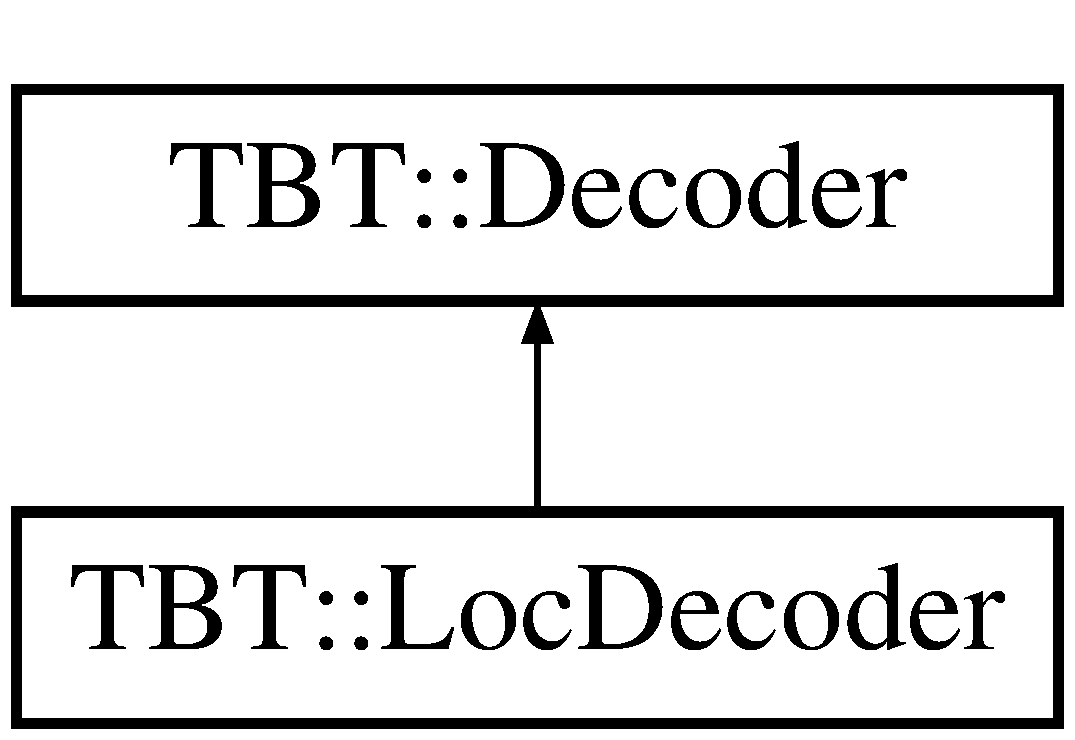
\includegraphics[height=2.000000cm]{classTBT_1_1Decoder}
\end{center}
\end{figure}
\subsection*{Public Member Functions}
\begin{DoxyCompactItemize}
\item 
\mbox{\Hypertarget{classTBT_1_1Decoder_a69cc50cb8ca993a98802303b1c70eade}\label{classTBT_1_1Decoder_a69cc50cb8ca993a98802303b1c70eade}} 
{\bfseries Decoder} (\hyperlink{classTBT_1_1Manager}{Manager} $\ast$p\+Manager, uint16\+\_\+t dcc\+Address)
\item 
\mbox{\Hypertarget{classTBT_1_1Decoder_ad948e489ff1246effdfda3e68d693593}\label{classTBT_1_1Decoder_ad948e489ff1246effdfda3e68d693593}} 
const uint16\+\_\+t {\bfseries get\+D\+C\+C\+Address} (void)
\item 
\mbox{\Hypertarget{classTBT_1_1Decoder_a71c25cd52e7f591ba1771ee0518735ba}\label{classTBT_1_1Decoder_a71c25cd52e7f591ba1771ee0518735ba}} 
virtual bool {\bfseries get\+Dcc\+Message} (uint8\+\_\+t $\ast$p\+Msg)
\end{DoxyCompactItemize}
\subsection*{Protected Attributes}
\begin{DoxyCompactItemize}
\item 
\mbox{\Hypertarget{classTBT_1_1Decoder_a14309179167dd46b722982301d651c4d}\label{classTBT_1_1Decoder_a14309179167dd46b722982301d651c4d}} 
uint16\+\_\+t {\bfseries m\+\_\+\+D\+C\+C\+Address}
\item 
\mbox{\Hypertarget{classTBT_1_1Decoder_a400475d21ba933f8b91e6f7d3053518b}\label{classTBT_1_1Decoder_a400475d21ba933f8b91e6f7d3053518b}} 
\hyperlink{classTBT_1_1Manager}{Manager} $\ast$ {\bfseries m\+\_\+p\+Manager}
\end{DoxyCompactItemize}


The documentation for this class was generated from the following files\+:\begin{DoxyCompactItemize}
\item 
Decoder.\+h\item 
Decoder.\+cpp\end{DoxyCompactItemize}

\hypertarget{classJson_1_1Exception}{}\section{Json\+:\+:Exception Class Reference}
\label{classJson_1_1Exception}\index{Json\+::\+Exception@{Json\+::\+Exception}}


{\ttfamily \#include $<$json.\+h$>$}

Inheritance diagram for Json\+:\+:Exception\+:\begin{figure}[H]
\begin{center}
\leavevmode
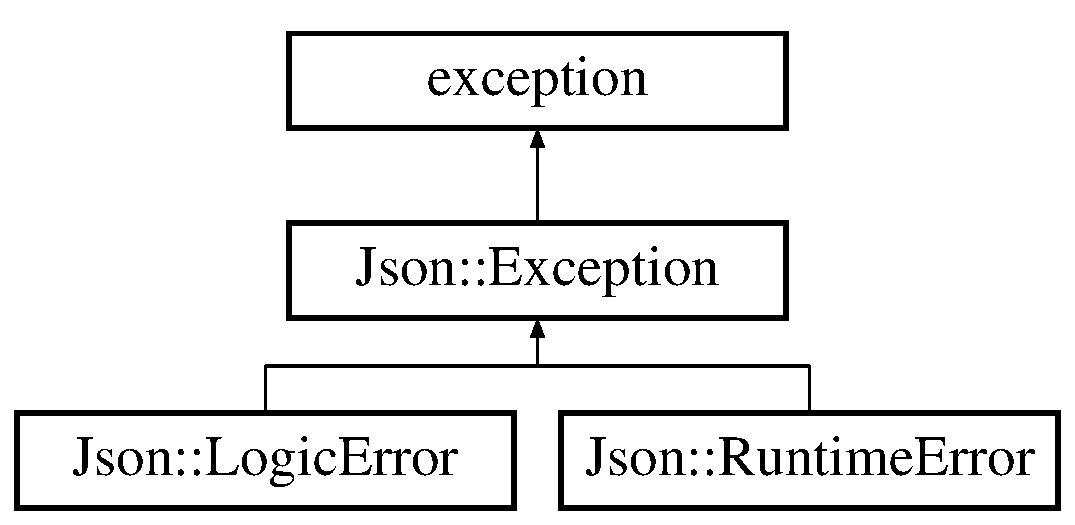
\includegraphics[height=3.000000cm]{classJson_1_1Exception}
\end{center}
\end{figure}
\subsection*{Public Member Functions}
\begin{DoxyCompactItemize}
\item 
\hyperlink{classJson_1_1Exception_ae764aa42e0755bd4ce9d303e2733fa8f_ae764aa42e0755bd4ce9d303e2733fa8f}{Exception} (\hyperlink{json_8h_a1e723f95759de062585bc4a8fd3fa4be_a1e723f95759de062585bc4a8fd3fa4be}{J\+S\+O\+N\+C\+P\+P\+\_\+\+S\+T\+R\+I\+NG} const \&msg)
\item 
\hyperlink{classJson_1_1Exception_add6af5e0ecdf36f40d7f3554b9786e21_add6af5e0ecdf36f40d7f3554b9786e21}{$\sim$\+Exception} () \hyperlink{json_8h_af8418c6d82d9de6e5f3c739fcf2fe88d_af8418c6d82d9de6e5f3c739fcf2fe88d}{J\+S\+O\+N\+C\+P\+P\+\_\+\+N\+O\+E\+X\+C\+E\+PT} \hyperlink{json_8h_a824d6199c91488107e443226fa6022c5_a824d6199c91488107e443226fa6022c5}{J\+S\+O\+N\+C\+P\+P\+\_\+\+O\+V\+E\+R\+R\+I\+DE}
\item 
char const  $\ast$ \hyperlink{classJson_1_1Exception_a70b7ce35e761fb93e8cd338e04619cd6_a70b7ce35e761fb93e8cd338e04619cd6}{what} () const \hyperlink{json_8h_af8418c6d82d9de6e5f3c739fcf2fe88d_af8418c6d82d9de6e5f3c739fcf2fe88d}{J\+S\+O\+N\+C\+P\+P\+\_\+\+N\+O\+E\+X\+C\+E\+PT} \hyperlink{json_8h_a824d6199c91488107e443226fa6022c5_a824d6199c91488107e443226fa6022c5}{J\+S\+O\+N\+C\+P\+P\+\_\+\+O\+V\+E\+R\+R\+I\+DE}
\end{DoxyCompactItemize}
\subsection*{Protected Attributes}
\begin{DoxyCompactItemize}
\item 
\hyperlink{json_8h_a1e723f95759de062585bc4a8fd3fa4be_a1e723f95759de062585bc4a8fd3fa4be}{J\+S\+O\+N\+C\+P\+P\+\_\+\+S\+T\+R\+I\+NG} \hyperlink{classJson_1_1Exception_aae3cbb8b45bf21480f64502a8329659f_aae3cbb8b45bf21480f64502a8329659f}{msg\+\_\+}
\end{DoxyCompactItemize}


\subsection{Detailed Description}
Base class for all exceptions we throw.

We use nothing but these internally. Of course, S\+TL can throw others. 

\subsection{Constructor \& Destructor Documentation}
\mbox{\Hypertarget{classJson_1_1Exception_ae764aa42e0755bd4ce9d303e2733fa8f_ae764aa42e0755bd4ce9d303e2733fa8f}\label{classJson_1_1Exception_ae764aa42e0755bd4ce9d303e2733fa8f_ae764aa42e0755bd4ce9d303e2733fa8f}} 
\index{Json\+::\+Exception@{Json\+::\+Exception}!Exception@{Exception}}
\index{Exception@{Exception}!Json\+::\+Exception@{Json\+::\+Exception}}
\subsubsection{\texorpdfstring{Exception()}{Exception()}}
{\footnotesize\ttfamily Json\+::\+Exception\+::\+Exception (\begin{DoxyParamCaption}\item[{\hyperlink{json_8h_a1e723f95759de062585bc4a8fd3fa4be_a1e723f95759de062585bc4a8fd3fa4be}{J\+S\+O\+N\+C\+P\+P\+\_\+\+S\+T\+R\+I\+NG} const \&}]{msg }\end{DoxyParamCaption})}

\mbox{\Hypertarget{classJson_1_1Exception_add6af5e0ecdf36f40d7f3554b9786e21_add6af5e0ecdf36f40d7f3554b9786e21}\label{classJson_1_1Exception_add6af5e0ecdf36f40d7f3554b9786e21_add6af5e0ecdf36f40d7f3554b9786e21}} 
\index{Json\+::\+Exception@{Json\+::\+Exception}!````~Exception@{$\sim$\+Exception}}
\index{````~Exception@{$\sim$\+Exception}!Json\+::\+Exception@{Json\+::\+Exception}}
\subsubsection{\texorpdfstring{$\sim$\+Exception()}{~Exception()}}
{\footnotesize\ttfamily Json\+::\+Exception\+::$\sim$\+Exception (\begin{DoxyParamCaption}{ }\end{DoxyParamCaption})}



\subsection{Member Function Documentation}
\mbox{\Hypertarget{classJson_1_1Exception_a70b7ce35e761fb93e8cd338e04619cd6_a70b7ce35e761fb93e8cd338e04619cd6}\label{classJson_1_1Exception_a70b7ce35e761fb93e8cd338e04619cd6_a70b7ce35e761fb93e8cd338e04619cd6}} 
\index{Json\+::\+Exception@{Json\+::\+Exception}!what@{what}}
\index{what@{what}!Json\+::\+Exception@{Json\+::\+Exception}}
\subsubsection{\texorpdfstring{what()}{what()}}
{\footnotesize\ttfamily char const  $\ast$ Json\+::\+Exception\+::what (\begin{DoxyParamCaption}{ }\end{DoxyParamCaption}) const}



References msg\+\_\+.



\subsection{Member Data Documentation}
\mbox{\Hypertarget{classJson_1_1Exception_aae3cbb8b45bf21480f64502a8329659f_aae3cbb8b45bf21480f64502a8329659f}\label{classJson_1_1Exception_aae3cbb8b45bf21480f64502a8329659f_aae3cbb8b45bf21480f64502a8329659f}} 
\index{Json\+::\+Exception@{Json\+::\+Exception}!msg\+\_\+@{msg\+\_\+}}
\index{msg\+\_\+@{msg\+\_\+}!Json\+::\+Exception@{Json\+::\+Exception}}
\subsubsection{\texorpdfstring{msg\+\_\+}{msg\_}}
{\footnotesize\ttfamily \hyperlink{json_8h_a1e723f95759de062585bc4a8fd3fa4be_a1e723f95759de062585bc4a8fd3fa4be}{J\+S\+O\+N\+C\+P\+P\+\_\+\+S\+T\+R\+I\+NG} Json\+::\+Exception\+::msg\+\_\+\hspace{0.3cm}{\ttfamily [protected]}}



Referenced by what().



The documentation for this class was generated from the following files\+:\begin{DoxyCompactItemize}
\item 
json/\hyperlink{json_8h}{json.\+h}\item 
\hyperlink{jsoncpp_8cpp}{jsoncpp.\+cpp}\end{DoxyCompactItemize}

\hypertarget{classJson_1_1CharReader_1_1Factory}{}\section{Json\+:\+:Char\+Reader\+:\+:Factory Class Reference}
\label{classJson_1_1CharReader_1_1Factory}\index{Json\+::\+Char\+Reader\+::\+Factory@{Json\+::\+Char\+Reader\+::\+Factory}}


{\ttfamily \#include $<$json.\+h$>$}

Inheritance diagram for Json\+:\+:Char\+Reader\+:\+:Factory\+:\begin{figure}[H]
\begin{center}
\leavevmode
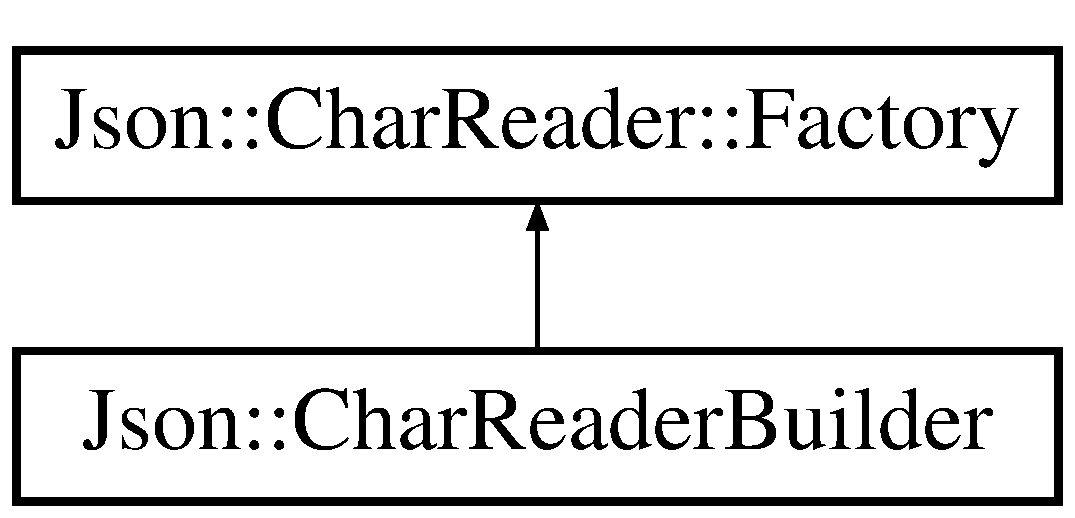
\includegraphics[height=2.000000cm]{classJson_1_1CharReader_1_1Factory}
\end{center}
\end{figure}
\subsection*{Public Member Functions}
\begin{DoxyCompactItemize}
\item 
virtual \hyperlink{classJson_1_1CharReader_1_1Factory_ae6938f632fa57f88e05818add5bc21be_ae6938f632fa57f88e05818add5bc21be}{$\sim$\+Factory} ()
\item 
virtual \hyperlink{classJson_1_1CharReader}{Char\+Reader} $\ast$ \hyperlink{classJson_1_1CharReader_1_1Factory_a4c5862a1ffd432372dbe65cf59de98c4_a4c5862a1ffd432372dbe65cf59de98c4}{new\+Char\+Reader} () const =0
\begin{DoxyCompactList}\small\item\em Allocate a \hyperlink{classJson_1_1CharReader}{Char\+Reader} via operator new(). \end{DoxyCompactList}\end{DoxyCompactItemize}


\subsection{Constructor \& Destructor Documentation}
\mbox{\Hypertarget{classJson_1_1CharReader_1_1Factory_ae6938f632fa57f88e05818add5bc21be_ae6938f632fa57f88e05818add5bc21be}\label{classJson_1_1CharReader_1_1Factory_ae6938f632fa57f88e05818add5bc21be_ae6938f632fa57f88e05818add5bc21be}} 
\index{Json\+::\+Char\+Reader\+::\+Factory@{Json\+::\+Char\+Reader\+::\+Factory}!````~Factory@{$\sim$\+Factory}}
\index{````~Factory@{$\sim$\+Factory}!Json\+::\+Char\+Reader\+::\+Factory@{Json\+::\+Char\+Reader\+::\+Factory}}
\subsubsection{\texorpdfstring{$\sim$\+Factory()}{~Factory()}}
{\footnotesize\ttfamily virtual Json\+::\+Char\+Reader\+::\+Factory\+::$\sim$\+Factory (\begin{DoxyParamCaption}{ }\end{DoxyParamCaption})\hspace{0.3cm}{\ttfamily [inline]}, {\ttfamily [virtual]}}



\subsection{Member Function Documentation}
\mbox{\Hypertarget{classJson_1_1CharReader_1_1Factory_a4c5862a1ffd432372dbe65cf59de98c4_a4c5862a1ffd432372dbe65cf59de98c4}\label{classJson_1_1CharReader_1_1Factory_a4c5862a1ffd432372dbe65cf59de98c4_a4c5862a1ffd432372dbe65cf59de98c4}} 
\index{Json\+::\+Char\+Reader\+::\+Factory@{Json\+::\+Char\+Reader\+::\+Factory}!new\+Char\+Reader@{new\+Char\+Reader}}
\index{new\+Char\+Reader@{new\+Char\+Reader}!Json\+::\+Char\+Reader\+::\+Factory@{Json\+::\+Char\+Reader\+::\+Factory}}
\subsubsection{\texorpdfstring{new\+Char\+Reader()}{newCharReader()}}
{\footnotesize\ttfamily virtual \hyperlink{classJson_1_1CharReader}{Char\+Reader}$\ast$ Json\+::\+Char\+Reader\+::\+Factory\+::new\+Char\+Reader (\begin{DoxyParamCaption}{ }\end{DoxyParamCaption}) const\hspace{0.3cm}{\ttfamily [pure virtual]}}



Allocate a \hyperlink{classJson_1_1CharReader}{Char\+Reader} via operator new(). 


\begin{DoxyExceptions}{Exceptions}
{\em std\+::exception} & if something goes wrong (e.\+g. invalid settings) \\
\hline
\end{DoxyExceptions}


Implemented in \hyperlink{classJson_1_1CharReaderBuilder_a3a262fcc76c1eb8eebfd4718fb4e9722_a3a262fcc76c1eb8eebfd4718fb4e9722}{Json\+::\+Char\+Reader\+Builder}.



Referenced by Json\+::parse\+From\+Stream().



The documentation for this class was generated from the following file\+:\begin{DoxyCompactItemize}
\item 
json/\hyperlink{json_8h}{json.\+h}\end{DoxyCompactItemize}

\hypertarget{classJson_1_1StreamWriter_1_1Factory}{}\section{Json\+:\+:Stream\+Writer\+:\+:Factory Class Reference}
\label{classJson_1_1StreamWriter_1_1Factory}\index{Json\+::\+Stream\+Writer\+::\+Factory@{Json\+::\+Stream\+Writer\+::\+Factory}}


A simple abstract factory.  




{\ttfamily \#include $<$json.\+h$>$}

Inheritance diagram for Json\+:\+:Stream\+Writer\+:\+:Factory\+:\begin{figure}[H]
\begin{center}
\leavevmode
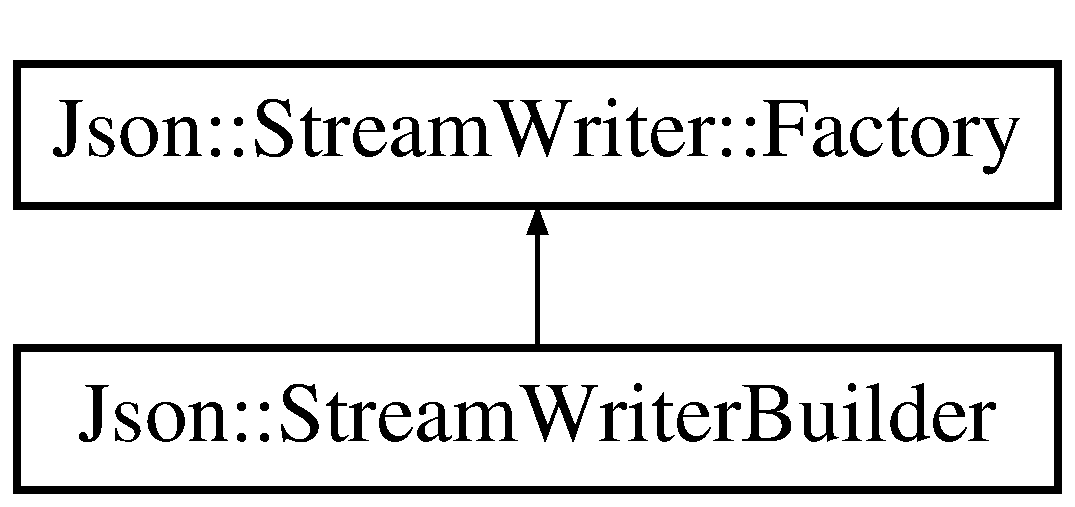
\includegraphics[height=2.000000cm]{classJson_1_1StreamWriter_1_1Factory}
\end{center}
\end{figure}
\subsection*{Public Member Functions}
\begin{DoxyCompactItemize}
\item 
virtual \hyperlink{classJson_1_1StreamWriter_1_1Factory_ad334ad5e81e3b9b1768620a446366ff1_ad334ad5e81e3b9b1768620a446366ff1}{$\sim$\+Factory} ()
\item 
virtual \hyperlink{classJson_1_1StreamWriter}{Stream\+Writer} $\ast$ \hyperlink{classJson_1_1StreamWriter_1_1Factory_a9d30ec53e8288cd53befccf1009c5f31_a9d30ec53e8288cd53befccf1009c5f31}{new\+Stream\+Writer} () const =0
\begin{DoxyCompactList}\small\item\em Allocate a \hyperlink{classJson_1_1CharReader}{Char\+Reader} via operator new(). \end{DoxyCompactList}\end{DoxyCompactItemize}


\subsection{Detailed Description}
A simple abstract factory. 

\subsection{Constructor \& Destructor Documentation}
\mbox{\Hypertarget{classJson_1_1StreamWriter_1_1Factory_ad334ad5e81e3b9b1768620a446366ff1_ad334ad5e81e3b9b1768620a446366ff1}\label{classJson_1_1StreamWriter_1_1Factory_ad334ad5e81e3b9b1768620a446366ff1_ad334ad5e81e3b9b1768620a446366ff1}} 
\index{Json\+::\+Stream\+Writer\+::\+Factory@{Json\+::\+Stream\+Writer\+::\+Factory}!````~Factory@{$\sim$\+Factory}}
\index{````~Factory@{$\sim$\+Factory}!Json\+::\+Stream\+Writer\+::\+Factory@{Json\+::\+Stream\+Writer\+::\+Factory}}
\subsubsection{\texorpdfstring{$\sim$\+Factory()}{~Factory()}}
{\footnotesize\ttfamily Json\+::\+Stream\+Writer\+::\+Factory\+::$\sim$\+Factory (\begin{DoxyParamCaption}{ }\end{DoxyParamCaption})\hspace{0.3cm}{\ttfamily [virtual]}}



\subsection{Member Function Documentation}
\mbox{\Hypertarget{classJson_1_1StreamWriter_1_1Factory_a9d30ec53e8288cd53befccf1009c5f31_a9d30ec53e8288cd53befccf1009c5f31}\label{classJson_1_1StreamWriter_1_1Factory_a9d30ec53e8288cd53befccf1009c5f31_a9d30ec53e8288cd53befccf1009c5f31}} 
\index{Json\+::\+Stream\+Writer\+::\+Factory@{Json\+::\+Stream\+Writer\+::\+Factory}!new\+Stream\+Writer@{new\+Stream\+Writer}}
\index{new\+Stream\+Writer@{new\+Stream\+Writer}!Json\+::\+Stream\+Writer\+::\+Factory@{Json\+::\+Stream\+Writer\+::\+Factory}}
\subsubsection{\texorpdfstring{new\+Stream\+Writer()}{newStreamWriter()}}
{\footnotesize\ttfamily virtual \hyperlink{classJson_1_1StreamWriter}{Stream\+Writer}$\ast$ Json\+::\+Stream\+Writer\+::\+Factory\+::new\+Stream\+Writer (\begin{DoxyParamCaption}{ }\end{DoxyParamCaption}) const\hspace{0.3cm}{\ttfamily [pure virtual]}}



Allocate a \hyperlink{classJson_1_1CharReader}{Char\+Reader} via operator new(). 


\begin{DoxyExceptions}{Exceptions}
{\em std\+::exception} & if something goes wrong (e.\+g. invalid settings) \\
\hline
\end{DoxyExceptions}


Implemented in \hyperlink{classJson_1_1StreamWriterBuilder_ab9ee278609f88ae04a7c1a84e1f559e6_ab9ee278609f88ae04a7c1a84e1f559e6}{Json\+::\+Stream\+Writer\+Builder}.



Referenced by Json\+::write\+String().



The documentation for this class was generated from the following files\+:\begin{DoxyCompactItemize}
\item 
json/\hyperlink{json_8h}{json.\+h}\item 
\hyperlink{jsoncpp_8cpp}{jsoncpp.\+cpp}\end{DoxyCompactItemize}

\hypertarget{classJson_1_1Features}{}\section{Json\+:\+:Features Class Reference}
\label{classJson_1_1Features}\index{Json\+::\+Features@{Json\+::\+Features}}


Configuration passed to reader and writer. This configuration object can be used to force the Reader or Writer to behave in a standard conforming way.  




{\ttfamily \#include $<$json.\+h$>$}

\subsection*{Public Member Functions}
\begin{DoxyCompactItemize}
\item 
\hyperlink{classJson_1_1Features_ad15a091cb61bb31323299a95970d2644_ad15a091cb61bb31323299a95970d2644}{Features} ()
\begin{DoxyCompactList}\small\item\em Initialize the configuration like Json\+Config\+::all\+Features;. \end{DoxyCompactList}\end{DoxyCompactItemize}
\subsection*{Static Public Member Functions}
\begin{DoxyCompactItemize}
\item 
static \hyperlink{classJson_1_1Features}{Features} \hyperlink{classJson_1_1Features_a63894da6e2c100b38741fa933f3d33ae_a63894da6e2c100b38741fa933f3d33ae}{all} ()
\begin{DoxyCompactList}\small\item\em A configuration that allows all features and assumes all strings are U\+T\+F-\/8. \end{DoxyCompactList}\item 
static \hyperlink{classJson_1_1Features}{Features} \hyperlink{classJson_1_1Features_ae23176c14b2e79e81fb61fb1a8ab58ee_ae23176c14b2e79e81fb61fb1a8ab58ee}{strict\+Mode} ()
\begin{DoxyCompactList}\small\item\em A configuration that is strictly compatible with the J\+S\+ON specification. \end{DoxyCompactList}\end{DoxyCompactItemize}
\subsection*{Public Attributes}
\begin{DoxyCompactItemize}
\item 
bool \hyperlink{classJson_1_1Features_a33afd389719624b6bdb23950b3c346c9_a33afd389719624b6bdb23950b3c346c9}{allow\+Comments\+\_\+}
\begin{DoxyCompactList}\small\item\em {\ttfamily true} if comments are allowed. Default\+: {\ttfamily true}. \end{DoxyCompactList}\item 
bool \hyperlink{classJson_1_1Features_a1162c37a1458adc32582b585b552f9c3_a1162c37a1458adc32582b585b552f9c3}{strict\+Root\+\_\+}
\item 
bool \hyperlink{classJson_1_1Features_a5076aa72c05c7596ac339ede36c97a6a_a5076aa72c05c7596ac339ede36c97a6a}{allow\+Dropped\+Null\+Placeholders\+\_\+}
\begin{DoxyCompactList}\small\item\em {\ttfamily true} if dropped null placeholders are allowed. Default\+: {\ttfamily false}. \end{DoxyCompactList}\item 
bool \hyperlink{classJson_1_1Features_aff3cb16b79d15d3d761b11a0dd6d4d6b_aff3cb16b79d15d3d761b11a0dd6d4d6b}{allow\+Numeric\+Keys\+\_\+}
\begin{DoxyCompactList}\small\item\em {\ttfamily true} if numeric object key are allowed. Default\+: {\ttfamily false}. \end{DoxyCompactList}\end{DoxyCompactItemize}


\subsection{Detailed Description}
Configuration passed to reader and writer. This configuration object can be used to force the Reader or Writer to behave in a standard conforming way. 

\subsection{Constructor \& Destructor Documentation}
\mbox{\Hypertarget{classJson_1_1Features_ad15a091cb61bb31323299a95970d2644_ad15a091cb61bb31323299a95970d2644}\label{classJson_1_1Features_ad15a091cb61bb31323299a95970d2644_ad15a091cb61bb31323299a95970d2644}} 
\index{Json\+::\+Features@{Json\+::\+Features}!Features@{Features}}
\index{Features@{Features}!Json\+::\+Features@{Json\+::\+Features}}
\subsubsection{\texorpdfstring{Features()}{Features()}}
{\footnotesize\ttfamily Json\+::\+Features\+::\+Features (\begin{DoxyParamCaption}{ }\end{DoxyParamCaption})}



Initialize the configuration like Json\+Config\+::all\+Features;. 



Referenced by all().



\subsection{Member Function Documentation}
\mbox{\Hypertarget{classJson_1_1Features_a63894da6e2c100b38741fa933f3d33ae_a63894da6e2c100b38741fa933f3d33ae}\label{classJson_1_1Features_a63894da6e2c100b38741fa933f3d33ae_a63894da6e2c100b38741fa933f3d33ae}} 
\index{Json\+::\+Features@{Json\+::\+Features}!all@{all}}
\index{all@{all}!Json\+::\+Features@{Json\+::\+Features}}
\subsubsection{\texorpdfstring{all()}{all()}}
{\footnotesize\ttfamily \hyperlink{classJson_1_1Features}{Features} Json\+::\+Features\+::all (\begin{DoxyParamCaption}{ }\end{DoxyParamCaption})\hspace{0.3cm}{\ttfamily [static]}}



A configuration that allows all features and assumes all strings are U\+T\+F-\/8. 


\begin{DoxyItemize}
\item C \& C++ comments are allowed
\item Root object can be any J\+S\+ON value
\item Assumes \hyperlink{classJson_1_1Value}{Value} strings are encoded in U\+T\+F-\/8 
\end{DoxyItemize}

References Features().



Referenced by strict\+Mode().

\mbox{\Hypertarget{classJson_1_1Features_ae23176c14b2e79e81fb61fb1a8ab58ee_ae23176c14b2e79e81fb61fb1a8ab58ee}\label{classJson_1_1Features_ae23176c14b2e79e81fb61fb1a8ab58ee_ae23176c14b2e79e81fb61fb1a8ab58ee}} 
\index{Json\+::\+Features@{Json\+::\+Features}!strict\+Mode@{strict\+Mode}}
\index{strict\+Mode@{strict\+Mode}!Json\+::\+Features@{Json\+::\+Features}}
\subsubsection{\texorpdfstring{strict\+Mode()}{strictMode()}}
{\footnotesize\ttfamily \hyperlink{classJson_1_1Features}{Features} Json\+::\+Features\+::strict\+Mode (\begin{DoxyParamCaption}{ }\end{DoxyParamCaption})\hspace{0.3cm}{\ttfamily [static]}}



A configuration that is strictly compatible with the J\+S\+ON specification. 


\begin{DoxyItemize}
\item Comments are forbidden.
\item Root object must be either an array or an object value.
\item Assumes \hyperlink{classJson_1_1Value}{Value} strings are encoded in U\+T\+F-\/8 
\end{DoxyItemize}

References all(), allow\+Comments\+\_\+, allow\+Dropped\+Null\+Placeholders\+\_\+, allow\+Numeric\+Keys\+\_\+, Json\+::array\+Value, Json\+::\+Value\+::as\+C\+String(), Json\+::code\+Point\+To\+U\+T\+F8(), Json\+::comment\+After, Json\+::comment\+After\+On\+Same\+Line, Json\+::comment\+Before, Json\+::\+Value\+::get\+Offset\+Limit(), Json\+::\+Value\+::get\+Offset\+Start(), Json\+::\+Value\+::is\+Array(), Json\+::\+Value\+::is\+Object(), J\+S\+O\+N\+C\+P\+P\+\_\+\+I\+S\+T\+R\+I\+N\+G\+S\+T\+R\+E\+AM, J\+S\+O\+N\+C\+P\+P\+\_\+\+S\+T\+R\+I\+NG, Json\+::\+Value\+::max\+Int, Json\+::\+Value\+::max\+Largest\+Int, Json\+::\+Value\+::max\+Largest\+U\+Int, Json\+::\+Value\+::min\+Largest\+Int, Json\+::object\+Value, Json\+::\+Value\+::set\+Comment(), stack\+Limit\+\_\+g, strict\+Root\+\_\+, Json\+::\+Value\+::swap\+Payload(), and Json\+::throw\+Runtime\+Error().



\subsection{Member Data Documentation}
\mbox{\Hypertarget{classJson_1_1Features_a33afd389719624b6bdb23950b3c346c9_a33afd389719624b6bdb23950b3c346c9}\label{classJson_1_1Features_a33afd389719624b6bdb23950b3c346c9_a33afd389719624b6bdb23950b3c346c9}} 
\index{Json\+::\+Features@{Json\+::\+Features}!allow\+Comments\+\_\+@{allow\+Comments\+\_\+}}
\index{allow\+Comments\+\_\+@{allow\+Comments\+\_\+}!Json\+::\+Features@{Json\+::\+Features}}
\subsubsection{\texorpdfstring{allow\+Comments\+\_\+}{allowComments\_}}
{\footnotesize\ttfamily bool Json\+::\+Features\+::allow\+Comments\+\_\+}



{\ttfamily true} if comments are allowed. Default\+: {\ttfamily true}. 



Referenced by strict\+Mode().

\mbox{\Hypertarget{classJson_1_1Features_a5076aa72c05c7596ac339ede36c97a6a_a5076aa72c05c7596ac339ede36c97a6a}\label{classJson_1_1Features_a5076aa72c05c7596ac339ede36c97a6a_a5076aa72c05c7596ac339ede36c97a6a}} 
\index{Json\+::\+Features@{Json\+::\+Features}!allow\+Dropped\+Null\+Placeholders\+\_\+@{allow\+Dropped\+Null\+Placeholders\+\_\+}}
\index{allow\+Dropped\+Null\+Placeholders\+\_\+@{allow\+Dropped\+Null\+Placeholders\+\_\+}!Json\+::\+Features@{Json\+::\+Features}}
\subsubsection{\texorpdfstring{allow\+Dropped\+Null\+Placeholders\+\_\+}{allowDroppedNullPlaceholders\_}}
{\footnotesize\ttfamily bool Json\+::\+Features\+::allow\+Dropped\+Null\+Placeholders\+\_\+}



{\ttfamily true} if dropped null placeholders are allowed. Default\+: {\ttfamily false}. 



Referenced by strict\+Mode().

\mbox{\Hypertarget{classJson_1_1Features_aff3cb16b79d15d3d761b11a0dd6d4d6b_aff3cb16b79d15d3d761b11a0dd6d4d6b}\label{classJson_1_1Features_aff3cb16b79d15d3d761b11a0dd6d4d6b_aff3cb16b79d15d3d761b11a0dd6d4d6b}} 
\index{Json\+::\+Features@{Json\+::\+Features}!allow\+Numeric\+Keys\+\_\+@{allow\+Numeric\+Keys\+\_\+}}
\index{allow\+Numeric\+Keys\+\_\+@{allow\+Numeric\+Keys\+\_\+}!Json\+::\+Features@{Json\+::\+Features}}
\subsubsection{\texorpdfstring{allow\+Numeric\+Keys\+\_\+}{allowNumericKeys\_}}
{\footnotesize\ttfamily bool Json\+::\+Features\+::allow\+Numeric\+Keys\+\_\+}



{\ttfamily true} if numeric object key are allowed. Default\+: {\ttfamily false}. 



Referenced by strict\+Mode().

\mbox{\Hypertarget{classJson_1_1Features_a1162c37a1458adc32582b585b552f9c3_a1162c37a1458adc32582b585b552f9c3}\label{classJson_1_1Features_a1162c37a1458adc32582b585b552f9c3_a1162c37a1458adc32582b585b552f9c3}} 
\index{Json\+::\+Features@{Json\+::\+Features}!strict\+Root\+\_\+@{strict\+Root\+\_\+}}
\index{strict\+Root\+\_\+@{strict\+Root\+\_\+}!Json\+::\+Features@{Json\+::\+Features}}
\subsubsection{\texorpdfstring{strict\+Root\+\_\+}{strictRoot\_}}
{\footnotesize\ttfamily bool Json\+::\+Features\+::strict\+Root\+\_\+}

{\ttfamily true} if root must be either an array or an object value. Default\+: {\ttfamily false}. 

Referenced by strict\+Mode().



The documentation for this class was generated from the following files\+:\begin{DoxyCompactItemize}
\item 
json/\hyperlink{json_8h}{json.\+h}\item 
\hyperlink{jsoncpp_8cpp}{jsoncpp.\+cpp}\end{DoxyCompactItemize}

\hypertarget{structhttp__message}{}\section{http\+\_\+message Struct Reference}
\label{structhttp__message}\index{http\+\_\+message@{http\+\_\+message}}
\subsection*{Public Attributes}
\begin{DoxyCompactItemize}
\item 
\mbox{\Hypertarget{structhttp__message_a005f4310b3d6f7f2c818e4dff1c81d10}\label{structhttp__message_a005f4310b3d6f7f2c818e4dff1c81d10}} 
struct \hyperlink{structmg__str}{mg\+\_\+str} {\bfseries message}
\item 
\mbox{\Hypertarget{structhttp__message_ab2e0f6d6abe3879d9f85238ae9c10fd5}\label{structhttp__message_ab2e0f6d6abe3879d9f85238ae9c10fd5}} 
struct \hyperlink{structmg__str}{mg\+\_\+str} {\bfseries body}
\item 
\mbox{\Hypertarget{structhttp__message_a446deffe0f2da170fb9216fd5c8812d2}\label{structhttp__message_a446deffe0f2da170fb9216fd5c8812d2}} 
struct \hyperlink{structmg__str}{mg\+\_\+str} {\bfseries method}
\item 
\mbox{\Hypertarget{structhttp__message_a2f8d9e674965443571fd6e581393dd62}\label{structhttp__message_a2f8d9e674965443571fd6e581393dd62}} 
struct \hyperlink{structmg__str}{mg\+\_\+str} {\bfseries uri}
\item 
\mbox{\Hypertarget{structhttp__message_aafd1525884e7c83d781d86c063ec1f4f}\label{structhttp__message_aafd1525884e7c83d781d86c063ec1f4f}} 
struct \hyperlink{structmg__str}{mg\+\_\+str} {\bfseries proto}
\item 
\mbox{\Hypertarget{structhttp__message_a1c4e12c873f1e4d9711d470e2e32fa65}\label{structhttp__message_a1c4e12c873f1e4d9711d470e2e32fa65}} 
int {\bfseries resp\+\_\+code}
\item 
\mbox{\Hypertarget{structhttp__message_ae819bf6100f781e15515c01bf03f5a76}\label{structhttp__message_ae819bf6100f781e15515c01bf03f5a76}} 
struct \hyperlink{structmg__str}{mg\+\_\+str} {\bfseries resp\+\_\+status\+\_\+msg}
\item 
\mbox{\Hypertarget{structhttp__message_a899c4cefcdda3ba4fbafcfb05a85bba5}\label{structhttp__message_a899c4cefcdda3ba4fbafcfb05a85bba5}} 
struct \hyperlink{structmg__str}{mg\+\_\+str} {\bfseries query\+\_\+string}
\item 
\mbox{\Hypertarget{structhttp__message_ad0a1f9898353bfcc80ab7f2f0a22adb0}\label{structhttp__message_ad0a1f9898353bfcc80ab7f2f0a22adb0}} 
struct \hyperlink{structmg__str}{mg\+\_\+str} {\bfseries header\+\_\+names} \mbox{[}M\+G\+\_\+\+M\+A\+X\+\_\+\+H\+T\+T\+P\+\_\+\+H\+E\+A\+D\+E\+RS\mbox{]}
\item 
\mbox{\Hypertarget{structhttp__message_a95a0bfefd3a05bb3db52ce50a2ef71f4}\label{structhttp__message_a95a0bfefd3a05bb3db52ce50a2ef71f4}} 
struct \hyperlink{structmg__str}{mg\+\_\+str} {\bfseries header\+\_\+values} \mbox{[}M\+G\+\_\+\+M\+A\+X\+\_\+\+H\+T\+T\+P\+\_\+\+H\+E\+A\+D\+E\+RS\mbox{]}
\end{DoxyCompactItemize}


The documentation for this struct was generated from the following file\+:\begin{DoxyCompactItemize}
\item 
mongoose.\+h\end{DoxyCompactItemize}

\hypertarget{classTBT_1_1LocDecoder}{}\section{T\+BT\+:\+:Loc\+Decoder Class Reference}
\label{classTBT_1_1LocDecoder}\index{T\+B\+T\+::\+Loc\+Decoder@{T\+B\+T\+::\+Loc\+Decoder}}
Inheritance diagram for T\+BT\+:\+:Loc\+Decoder\+:\begin{figure}[H]
\begin{center}
\leavevmode
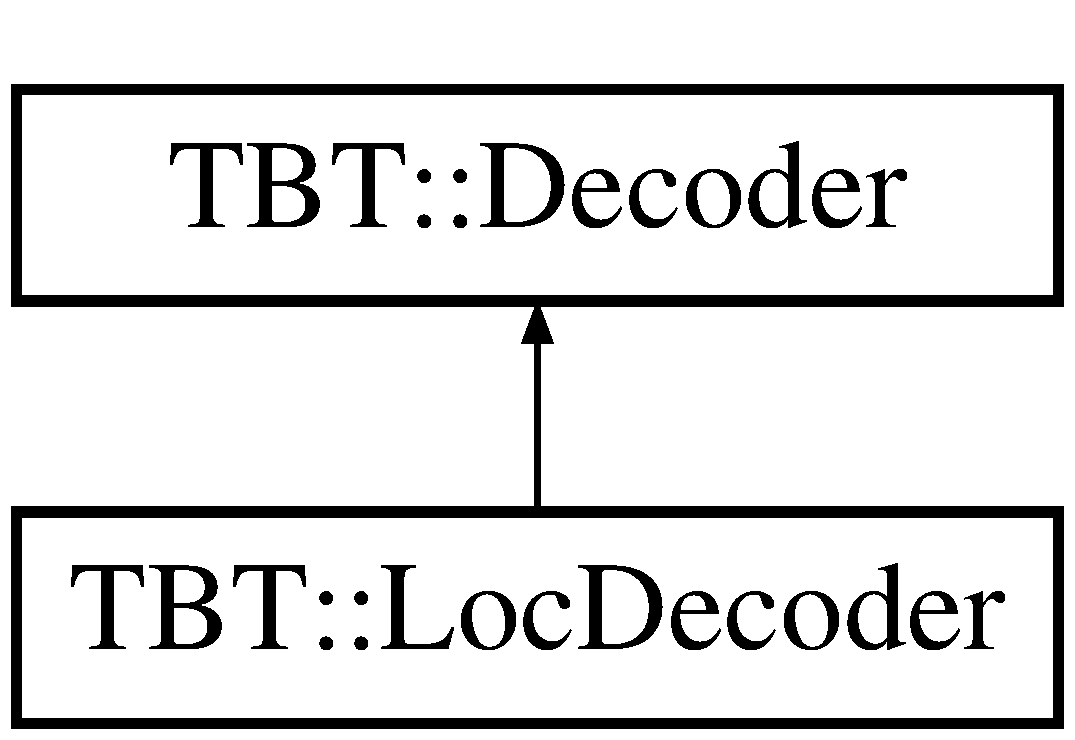
\includegraphics[height=2.000000cm]{classTBT_1_1LocDecoder}
\end{center}
\end{figure}
\subsection*{Public Member Functions}
\begin{DoxyCompactItemize}
\item 
\mbox{\Hypertarget{classTBT_1_1LocDecoder_ae8563de74c15f27c40644bf8218d26d9}\label{classTBT_1_1LocDecoder_ae8563de74c15f27c40644bf8218d26d9}} 
{\bfseries Loc\+Decoder} (\hyperlink{classTBT_1_1Manager}{Manager} $\ast$p\+Manager, uint16\+\_\+t dcc\+Address)
\item 
\mbox{\Hypertarget{classTBT_1_1LocDecoder_afaa04ad0561a39212d69d0aabece751e}\label{classTBT_1_1LocDecoder_afaa04ad0561a39212d69d0aabece751e}} 
uint8\+\_\+t {\bfseries get\+Loc\+Mode} (void)
\item 
\mbox{\Hypertarget{classTBT_1_1LocDecoder_a257c294961f07e5f2134b1550355a661}\label{classTBT_1_1LocDecoder_a257c294961f07e5f2134b1550355a661}} 
void {\bfseries get\+L\+A\+N\+Loc\+Info} (uint8\+\_\+t $\ast$p\+Msg)
\item 
\mbox{\Hypertarget{classTBT_1_1LocDecoder_a0ed2026cd64ba1e2aa411e1228027f4e}\label{classTBT_1_1LocDecoder_a0ed2026cd64ba1e2aa411e1228027f4e}} 
uint8\+\_\+t {\bfseries set\+Loc\+Mode} (uint8\+\_\+t new\+Mode)
\item 
\mbox{\Hypertarget{classTBT_1_1LocDecoder_a3ec11c7c270d1eeb00e6893bff8f0831}\label{classTBT_1_1LocDecoder_a3ec11c7c270d1eeb00e6893bff8f0831}} 
bool {\bfseries get\+Busy} ()
\item 
\mbox{\Hypertarget{classTBT_1_1LocDecoder_ae89a770202444bca60595182fe4a9c90}\label{classTBT_1_1LocDecoder_ae89a770202444bca60595182fe4a9c90}} 
uint8\+\_\+t {\bfseries get\+Speedsteps} ()
\item 
\mbox{\Hypertarget{classTBT_1_1LocDecoder_a5c570e65adde5ee526986155d509da47}\label{classTBT_1_1LocDecoder_a5c570e65adde5ee526986155d509da47}} 
bool {\bfseries get\+Direction} ()
\item 
\mbox{\Hypertarget{classTBT_1_1LocDecoder_a7305c8ab02a76b48b2b5ab93f1aec24b}\label{classTBT_1_1LocDecoder_a7305c8ab02a76b48b2b5ab93f1aec24b}} 
uint8\+\_\+t {\bfseries get\+Speed} ()
\item 
\mbox{\Hypertarget{classTBT_1_1LocDecoder_a7f4c04a5a306ea827494b29789cc401e}\label{classTBT_1_1LocDecoder_a7f4c04a5a306ea827494b29789cc401e}} 
bool {\bfseries get\+Dual\+Traction} ()
\item 
\mbox{\Hypertarget{classTBT_1_1LocDecoder_ab0a2b2953657fbc2589f90918883d03a}\label{classTBT_1_1LocDecoder_ab0a2b2953657fbc2589f90918883d03a}} 
bool {\bfseries get\+Smart\+Search} ()
\item 
\mbox{\Hypertarget{classTBT_1_1LocDecoder_a14a2d03a9f667ebfc4472fab880271b7}\label{classTBT_1_1LocDecoder_a14a2d03a9f667ebfc4472fab880271b7}} 
bool {\bfseries get\+Light} ()
\item 
\mbox{\Hypertarget{classTBT_1_1LocDecoder_ad659466bfea38d48902183acd6c450ab}\label{classTBT_1_1LocDecoder_ad659466bfea38d48902183acd6c450ab}} 
uint8\+\_\+t {\bfseries get\+Function\+Group1} ()
\item 
\mbox{\Hypertarget{classTBT_1_1LocDecoder_add8099fb79a671d02eeb993358f237fc}\label{classTBT_1_1LocDecoder_add8099fb79a671d02eeb993358f237fc}} 
bool {\bfseries get\+F0} ()
\item 
\mbox{\Hypertarget{classTBT_1_1LocDecoder_a583ff5f16d5b22d41be688b788f928bf}\label{classTBT_1_1LocDecoder_a583ff5f16d5b22d41be688b788f928bf}} 
bool {\bfseries get\+F1} ()
\item 
\mbox{\Hypertarget{classTBT_1_1LocDecoder_a1ed926bf58e50df8dd8650f268c26b6f}\label{classTBT_1_1LocDecoder_a1ed926bf58e50df8dd8650f268c26b6f}} 
bool {\bfseries get\+F2} ()
\item 
\mbox{\Hypertarget{classTBT_1_1LocDecoder_a421ae56808383dbc63de19b21c08fb5d}\label{classTBT_1_1LocDecoder_a421ae56808383dbc63de19b21c08fb5d}} 
bool {\bfseries get\+F3} ()
\item 
\mbox{\Hypertarget{classTBT_1_1LocDecoder_a2af90878d4f8f1f3b64f393519ac8f7a}\label{classTBT_1_1LocDecoder_a2af90878d4f8f1f3b64f393519ac8f7a}} 
bool {\bfseries get\+F4} ()
\item 
\mbox{\Hypertarget{classTBT_1_1LocDecoder_a5a23ba503d7b4798ac8c00019e4d3557}\label{classTBT_1_1LocDecoder_a5a23ba503d7b4798ac8c00019e4d3557}} 
uint8\+\_\+t {\bfseries get\+Function\+Group2} ()
\item 
\mbox{\Hypertarget{classTBT_1_1LocDecoder_a25b602fa8075cd6eb22bb936d9e957c7}\label{classTBT_1_1LocDecoder_a25b602fa8075cd6eb22bb936d9e957c7}} 
bool {\bfseries get\+F5} ()
\item 
\mbox{\Hypertarget{classTBT_1_1LocDecoder_a41b96104eec97905909c8c99c20756e5}\label{classTBT_1_1LocDecoder_a41b96104eec97905909c8c99c20756e5}} 
bool {\bfseries get\+F6} ()
\item 
\mbox{\Hypertarget{classTBT_1_1LocDecoder_a3f0a6c199b8222c53f047bd32f9060fc}\label{classTBT_1_1LocDecoder_a3f0a6c199b8222c53f047bd32f9060fc}} 
bool {\bfseries get\+F7} ()
\item 
\mbox{\Hypertarget{classTBT_1_1LocDecoder_ade02f20fc47f75a60a16f5f14339f7a1}\label{classTBT_1_1LocDecoder_ade02f20fc47f75a60a16f5f14339f7a1}} 
bool {\bfseries get\+F8} ()
\item 
\mbox{\Hypertarget{classTBT_1_1LocDecoder_a756c41f02751356fb934252b20c8b0f0}\label{classTBT_1_1LocDecoder_a756c41f02751356fb934252b20c8b0f0}} 
uint8\+\_\+t {\bfseries get\+Function\+Group3} ()
\item 
\mbox{\Hypertarget{classTBT_1_1LocDecoder_adfbe30b0ab41b8a126514938d98b3222}\label{classTBT_1_1LocDecoder_adfbe30b0ab41b8a126514938d98b3222}} 
bool {\bfseries get\+F9} ()
\item 
\mbox{\Hypertarget{classTBT_1_1LocDecoder_ac891adfab9ecf9ca3dec29d387698c30}\label{classTBT_1_1LocDecoder_ac891adfab9ecf9ca3dec29d387698c30}} 
bool {\bfseries get\+F10} ()
\item 
\mbox{\Hypertarget{classTBT_1_1LocDecoder_af3beee6516b8af8046b469d6326250b1}\label{classTBT_1_1LocDecoder_af3beee6516b8af8046b469d6326250b1}} 
bool {\bfseries get\+F11} ()
\item 
\mbox{\Hypertarget{classTBT_1_1LocDecoder_aa9ff3866964a5a6be01d6a6c22498b9d}\label{classTBT_1_1LocDecoder_aa9ff3866964a5a6be01d6a6c22498b9d}} 
bool {\bfseries get\+F12} ()
\item 
\mbox{\Hypertarget{classTBT_1_1LocDecoder_ab3f960f23613062dd97a3fb2274ee02c}\label{classTBT_1_1LocDecoder_ab3f960f23613062dd97a3fb2274ee02c}} 
uint8\+\_\+t {\bfseries get\+Function\+Group4} ()
\item 
\mbox{\Hypertarget{classTBT_1_1LocDecoder_aeca11289c531630bcecf39fd747d97b4}\label{classTBT_1_1LocDecoder_aeca11289c531630bcecf39fd747d97b4}} 
bool {\bfseries get\+F13} ()
\item 
\mbox{\Hypertarget{classTBT_1_1LocDecoder_a839308828d5775da64621292caa07651}\label{classTBT_1_1LocDecoder_a839308828d5775da64621292caa07651}} 
bool {\bfseries get\+F14} ()
\item 
\mbox{\Hypertarget{classTBT_1_1LocDecoder_a4bcfbf55ed042a80d5b045eb7915234a}\label{classTBT_1_1LocDecoder_a4bcfbf55ed042a80d5b045eb7915234a}} 
bool {\bfseries get\+F15} ()
\item 
\mbox{\Hypertarget{classTBT_1_1LocDecoder_a11aa0521314deb69fd50d44eb9f35d8d}\label{classTBT_1_1LocDecoder_a11aa0521314deb69fd50d44eb9f35d8d}} 
bool {\bfseries get\+F16} ()
\item 
\mbox{\Hypertarget{classTBT_1_1LocDecoder_a3197258036f35718c884aba8df521b54}\label{classTBT_1_1LocDecoder_a3197258036f35718c884aba8df521b54}} 
bool {\bfseries get\+F17} ()
\item 
\mbox{\Hypertarget{classTBT_1_1LocDecoder_a8a0533187d68e90e5a616dbcc934a111}\label{classTBT_1_1LocDecoder_a8a0533187d68e90e5a616dbcc934a111}} 
bool {\bfseries get\+F18} ()
\item 
\mbox{\Hypertarget{classTBT_1_1LocDecoder_ad61a122b7e69336f878baa2f5670a4e8}\label{classTBT_1_1LocDecoder_ad61a122b7e69336f878baa2f5670a4e8}} 
bool {\bfseries get\+F19} ()
\item 
\mbox{\Hypertarget{classTBT_1_1LocDecoder_abcb11e56a79e9229212139723630aef0}\label{classTBT_1_1LocDecoder_abcb11e56a79e9229212139723630aef0}} 
bool {\bfseries get\+F20} ()
\item 
\mbox{\Hypertarget{classTBT_1_1LocDecoder_aac83243e509961ce7eedb9959fcecb73}\label{classTBT_1_1LocDecoder_aac83243e509961ce7eedb9959fcecb73}} 
uint8\+\_\+t {\bfseries get\+Function\+Group5} ()
\item 
\mbox{\Hypertarget{classTBT_1_1LocDecoder_a89ea694d153a4f68ffe7df1f37fd7fc6}\label{classTBT_1_1LocDecoder_a89ea694d153a4f68ffe7df1f37fd7fc6}} 
bool {\bfseries get\+F21} ()
\item 
\mbox{\Hypertarget{classTBT_1_1LocDecoder_a9d95d2ac3b1079b9ffa519440808d4e2}\label{classTBT_1_1LocDecoder_a9d95d2ac3b1079b9ffa519440808d4e2}} 
bool {\bfseries get\+F22} ()
\item 
\mbox{\Hypertarget{classTBT_1_1LocDecoder_ab03cf89a7d635e61ebb1362f5f8274fc}\label{classTBT_1_1LocDecoder_ab03cf89a7d635e61ebb1362f5f8274fc}} 
bool {\bfseries get\+F23} ()
\item 
\mbox{\Hypertarget{classTBT_1_1LocDecoder_a16317eca85676a89372298782c71c6cb}\label{classTBT_1_1LocDecoder_a16317eca85676a89372298782c71c6cb}} 
bool {\bfseries get\+F24} ()
\item 
\mbox{\Hypertarget{classTBT_1_1LocDecoder_a3e06e61df29ee70660c003cbe81cb497}\label{classTBT_1_1LocDecoder_a3e06e61df29ee70660c003cbe81cb497}} 
bool {\bfseries get\+F25} ()
\item 
\mbox{\Hypertarget{classTBT_1_1LocDecoder_aa240dc8548525b91d931eed9cd549657}\label{classTBT_1_1LocDecoder_aa240dc8548525b91d931eed9cd549657}} 
bool {\bfseries get\+F26} ()
\item 
\mbox{\Hypertarget{classTBT_1_1LocDecoder_a0f8abd84b95094b2a139bd3402153aae}\label{classTBT_1_1LocDecoder_a0f8abd84b95094b2a139bd3402153aae}} 
bool {\bfseries get\+F27} ()
\item 
\mbox{\Hypertarget{classTBT_1_1LocDecoder_aecb2127b4edc17aac10dda93b4404e1d}\label{classTBT_1_1LocDecoder_aecb2127b4edc17aac10dda93b4404e1d}} 
bool {\bfseries get\+F28} ()
\item 
\mbox{\Hypertarget{classTBT_1_1LocDecoder_ac8f62e05b5ea28dcbaf1c07a1c4a91ec}\label{classTBT_1_1LocDecoder_ac8f62e05b5ea28dcbaf1c07a1c4a91ec}} 
void {\bfseries set\+Busy} (bool value)
\item 
\mbox{\Hypertarget{classTBT_1_1LocDecoder_aa919a313cb33a49d792694a544f2d3de}\label{classTBT_1_1LocDecoder_aa919a313cb33a49d792694a544f2d3de}} 
void {\bfseries set\+Speedsteps} (uint8\+\_\+t value)
\item 
\mbox{\Hypertarget{classTBT_1_1LocDecoder_a5b0ba8089edaf920fb513e26701580bf}\label{classTBT_1_1LocDecoder_a5b0ba8089edaf920fb513e26701580bf}} 
void {\bfseries set\+Loco\+Drive14} (uint8\+\_\+t value)
\item 
\mbox{\Hypertarget{classTBT_1_1LocDecoder_ace59dd8679514643328ce916057669e4}\label{classTBT_1_1LocDecoder_ace59dd8679514643328ce916057669e4}} 
void {\bfseries set\+Loco\+Drive27} (uint8\+\_\+t value)
\item 
\mbox{\Hypertarget{classTBT_1_1LocDecoder_a6bbf6c173217c49b7d4909b9c4cb5127}\label{classTBT_1_1LocDecoder_a6bbf6c173217c49b7d4909b9c4cb5127}} 
void {\bfseries set\+Loco\+Drive28} (uint8\+\_\+t value)
\item 
\mbox{\Hypertarget{classTBT_1_1LocDecoder_a9de246d419829f424e8b50c817c599ca}\label{classTBT_1_1LocDecoder_a9de246d419829f424e8b50c817c599ca}} 
void {\bfseries set\+Loco\+Drive128} (uint8\+\_\+t value)
\item 
\mbox{\Hypertarget{classTBT_1_1LocDecoder_a7e5a054cecfa15cc2574b166c2001deb}\label{classTBT_1_1LocDecoder_a7e5a054cecfa15cc2574b166c2001deb}} 
void {\bfseries set\+Direction} (bool value)
\item 
\mbox{\Hypertarget{classTBT_1_1LocDecoder_afa7b68a8e717065e39c80a83cbd9bb66}\label{classTBT_1_1LocDecoder_afa7b68a8e717065e39c80a83cbd9bb66}} 
void {\bfseries set\+Speed} (uint8\+\_\+t value)
\item 
\mbox{\Hypertarget{classTBT_1_1LocDecoder_a1dbc0fcca21619d0283e1a61bbb1f7b2}\label{classTBT_1_1LocDecoder_a1dbc0fcca21619d0283e1a61bbb1f7b2}} 
void {\bfseries set\+Dual\+Traction} (bool value)
\item 
\mbox{\Hypertarget{classTBT_1_1LocDecoder_ab17b176f9fb53af19911611dc35c4e76}\label{classTBT_1_1LocDecoder_ab17b176f9fb53af19911611dc35c4e76}} 
void {\bfseries set\+Smart\+Search} (bool value)
\item 
\mbox{\Hypertarget{classTBT_1_1LocDecoder_a7d77fa29a27f1abff7dba21c3cca7ff1}\label{classTBT_1_1LocDecoder_a7d77fa29a27f1abff7dba21c3cca7ff1}} 
void {\bfseries set\+Function\+Group1} (const uint8\+\_\+t \&value)
\item 
\mbox{\Hypertarget{classTBT_1_1LocDecoder_a71807a8bab2731cc511659f118ecb01a}\label{classTBT_1_1LocDecoder_a71807a8bab2731cc511659f118ecb01a}} 
void {\bfseries set\+Light} (bool value)
\item 
\mbox{\Hypertarget{classTBT_1_1LocDecoder_ae7dc2a2221ba08ecaf34f50636f59b54}\label{classTBT_1_1LocDecoder_ae7dc2a2221ba08ecaf34f50636f59b54}} 
void {\bfseries set\+F0} (bool value)
\item 
\mbox{\Hypertarget{classTBT_1_1LocDecoder_aba76c6a9b002224297ba04ded570eee4}\label{classTBT_1_1LocDecoder_aba76c6a9b002224297ba04ded570eee4}} 
void {\bfseries set\+F1} (bool value)
\item 
\mbox{\Hypertarget{classTBT_1_1LocDecoder_a60e4822d5d730abec02cf045353d5316}\label{classTBT_1_1LocDecoder_a60e4822d5d730abec02cf045353d5316}} 
void {\bfseries set\+F2} (bool value)
\item 
\mbox{\Hypertarget{classTBT_1_1LocDecoder_a6316b9510a9f3552dae834bb6c3deebc}\label{classTBT_1_1LocDecoder_a6316b9510a9f3552dae834bb6c3deebc}} 
void {\bfseries set\+F3} (bool value)
\item 
\mbox{\Hypertarget{classTBT_1_1LocDecoder_ae37228489df216238a51e1a22c37d66c}\label{classTBT_1_1LocDecoder_ae37228489df216238a51e1a22c37d66c}} 
void {\bfseries set\+F4} (bool value)
\item 
\mbox{\Hypertarget{classTBT_1_1LocDecoder_af021433df427aac432590da7be6393a8}\label{classTBT_1_1LocDecoder_af021433df427aac432590da7be6393a8}} 
void {\bfseries set\+Function\+Group2} (const uint8\+\_\+t \&value)
\item 
\mbox{\Hypertarget{classTBT_1_1LocDecoder_a4e548e580a6ec3c93369af591281e00f}\label{classTBT_1_1LocDecoder_a4e548e580a6ec3c93369af591281e00f}} 
void {\bfseries set\+F5} (bool value)
\item 
\mbox{\Hypertarget{classTBT_1_1LocDecoder_af971c14a9437b240d17ab4ca9ffb3e67}\label{classTBT_1_1LocDecoder_af971c14a9437b240d17ab4ca9ffb3e67}} 
void {\bfseries set\+F6} (bool value)
\item 
\mbox{\Hypertarget{classTBT_1_1LocDecoder_a16a3659cd9a64be4b6ef43b499004434}\label{classTBT_1_1LocDecoder_a16a3659cd9a64be4b6ef43b499004434}} 
void {\bfseries set\+F7} (bool value)
\item 
\mbox{\Hypertarget{classTBT_1_1LocDecoder_a6a65d02e101d91142ce48587c9c905cf}\label{classTBT_1_1LocDecoder_a6a65d02e101d91142ce48587c9c905cf}} 
void {\bfseries set\+F8} (bool value)
\item 
\mbox{\Hypertarget{classTBT_1_1LocDecoder_a81f9805d0a984a94dab529602ef9ae64}\label{classTBT_1_1LocDecoder_a81f9805d0a984a94dab529602ef9ae64}} 
void {\bfseries set\+Function\+Group3} (const uint8\+\_\+t \&value)
\item 
\mbox{\Hypertarget{classTBT_1_1LocDecoder_a725b9d78cbdbd1e60a9102ddf5b8aaf3}\label{classTBT_1_1LocDecoder_a725b9d78cbdbd1e60a9102ddf5b8aaf3}} 
void {\bfseries set\+F9} (bool value)
\item 
\mbox{\Hypertarget{classTBT_1_1LocDecoder_a9976487964f6167d2d5e084d4ed787b7}\label{classTBT_1_1LocDecoder_a9976487964f6167d2d5e084d4ed787b7}} 
void {\bfseries set\+F10} (bool value)
\item 
\mbox{\Hypertarget{classTBT_1_1LocDecoder_aa732b54dfa7d535cec4aaab105f4c64d}\label{classTBT_1_1LocDecoder_aa732b54dfa7d535cec4aaab105f4c64d}} 
void {\bfseries set\+F11} (bool value)
\item 
\mbox{\Hypertarget{classTBT_1_1LocDecoder_a8b7c59df79fb92011db6e5e5999ffd28}\label{classTBT_1_1LocDecoder_a8b7c59df79fb92011db6e5e5999ffd28}} 
void {\bfseries set\+F12} (bool value)
\item 
\mbox{\Hypertarget{classTBT_1_1LocDecoder_a5b7c569ddccfe68faef7136bf27fadb8}\label{classTBT_1_1LocDecoder_a5b7c569ddccfe68faef7136bf27fadb8}} 
void {\bfseries set\+Function\+Group4} (const uint8\+\_\+t \&value)
\item 
\mbox{\Hypertarget{classTBT_1_1LocDecoder_a90966aa043e13a5f2a8c4f4019c662c9}\label{classTBT_1_1LocDecoder_a90966aa043e13a5f2a8c4f4019c662c9}} 
void {\bfseries set\+F13} (bool value)
\item 
\mbox{\Hypertarget{classTBT_1_1LocDecoder_a4d74e6b1232f3c716bf624dc1681164a}\label{classTBT_1_1LocDecoder_a4d74e6b1232f3c716bf624dc1681164a}} 
void {\bfseries set\+F14} (bool value)
\item 
\mbox{\Hypertarget{classTBT_1_1LocDecoder_aee5779bd1917c16099c77b3d57aedbb8}\label{classTBT_1_1LocDecoder_aee5779bd1917c16099c77b3d57aedbb8}} 
void {\bfseries set\+F15} (bool value)
\item 
\mbox{\Hypertarget{classTBT_1_1LocDecoder_a0a1a0f36dbe6b3c0c50eda41eb7b673e}\label{classTBT_1_1LocDecoder_a0a1a0f36dbe6b3c0c50eda41eb7b673e}} 
void {\bfseries set\+F16} (bool value)
\item 
\mbox{\Hypertarget{classTBT_1_1LocDecoder_ad1355610f7158630e75af3df1e4d01c4}\label{classTBT_1_1LocDecoder_ad1355610f7158630e75af3df1e4d01c4}} 
void {\bfseries set\+F17} (bool value)
\item 
\mbox{\Hypertarget{classTBT_1_1LocDecoder_aae4349cafcf17f8530ce151507bf3cf3}\label{classTBT_1_1LocDecoder_aae4349cafcf17f8530ce151507bf3cf3}} 
void {\bfseries set\+F18} (bool value)
\item 
\mbox{\Hypertarget{classTBT_1_1LocDecoder_a4625176dfddd8495f7a11be4b9dd29bf}\label{classTBT_1_1LocDecoder_a4625176dfddd8495f7a11be4b9dd29bf}} 
void {\bfseries set\+F19} (bool value)
\item 
\mbox{\Hypertarget{classTBT_1_1LocDecoder_a04a0514ad5b63714ca5774cf3c2e277c}\label{classTBT_1_1LocDecoder_a04a0514ad5b63714ca5774cf3c2e277c}} 
void {\bfseries set\+F20} (bool value)
\item 
\mbox{\Hypertarget{classTBT_1_1LocDecoder_a30659350a469bda322d276ee17b1b89c}\label{classTBT_1_1LocDecoder_a30659350a469bda322d276ee17b1b89c}} 
void {\bfseries set\+Function\+Group5} (const uint8\+\_\+t \&value)
\item 
\mbox{\Hypertarget{classTBT_1_1LocDecoder_ab5d79049ab7e38b4d408c9627db99a6d}\label{classTBT_1_1LocDecoder_ab5d79049ab7e38b4d408c9627db99a6d}} 
void {\bfseries set\+F21} (bool value)
\item 
\mbox{\Hypertarget{classTBT_1_1LocDecoder_a7dc0125781c063f15dda51d03ec3e25d}\label{classTBT_1_1LocDecoder_a7dc0125781c063f15dda51d03ec3e25d}} 
void {\bfseries set\+F22} (bool value)
\item 
\mbox{\Hypertarget{classTBT_1_1LocDecoder_a7b5a668ba542b1d8a8b47064be1f5c5a}\label{classTBT_1_1LocDecoder_a7b5a668ba542b1d8a8b47064be1f5c5a}} 
void {\bfseries set\+F23} (bool value)
\item 
\mbox{\Hypertarget{classTBT_1_1LocDecoder_a3c44b57443b1d600380ccf8e55da23e5}\label{classTBT_1_1LocDecoder_a3c44b57443b1d600380ccf8e55da23e5}} 
void {\bfseries set\+F24} (bool value)
\item 
\mbox{\Hypertarget{classTBT_1_1LocDecoder_aafefc743964ea0b01ff3ad51fee98033}\label{classTBT_1_1LocDecoder_aafefc743964ea0b01ff3ad51fee98033}} 
void {\bfseries set\+F25} (bool value)
\item 
\mbox{\Hypertarget{classTBT_1_1LocDecoder_a646c6edc6515dadaebac9b06a0907a9e}\label{classTBT_1_1LocDecoder_a646c6edc6515dadaebac9b06a0907a9e}} 
void {\bfseries set\+F26} (bool value)
\item 
\mbox{\Hypertarget{classTBT_1_1LocDecoder_a7584ffb3eaf00b83b48217081049ff59}\label{classTBT_1_1LocDecoder_a7584ffb3eaf00b83b48217081049ff59}} 
void {\bfseries set\+F27} (bool value)
\item 
\mbox{\Hypertarget{classTBT_1_1LocDecoder_a66c6f1dcd471f19d019018ed3eed2e0f}\label{classTBT_1_1LocDecoder_a66c6f1dcd471f19d019018ed3eed2e0f}} 
void {\bfseries set\+F28} (bool value)
\end{DoxyCompactItemize}
\subsection*{Protected Attributes}
\begin{DoxyCompactItemize}
\item 
\mbox{\Hypertarget{classTBT_1_1LocDecoder_a196fc5289b1ea2c9439b385770692c92}\label{classTBT_1_1LocDecoder_a196fc5289b1ea2c9439b385770692c92}} 
uint8\+\_\+t {\bfseries m\+\_\+\+Loc\+Mode}
\end{DoxyCompactItemize}


The documentation for this class was generated from the following files\+:\begin{DoxyCompactItemize}
\item 
Loc\+Decoder.\+h\item 
Loc\+Decoder.\+cpp\end{DoxyCompactItemize}

\hypertarget{classJson_1_1LogicError}{}\section{Json\+:\+:Logic\+Error Class Reference}
\label{classJson_1_1LogicError}\index{Json\+::\+Logic\+Error@{Json\+::\+Logic\+Error}}


{\ttfamily \#include $<$json.\+h$>$}

Inheritance diagram for Json\+:\+:Logic\+Error\+:\begin{figure}[H]
\begin{center}
\leavevmode
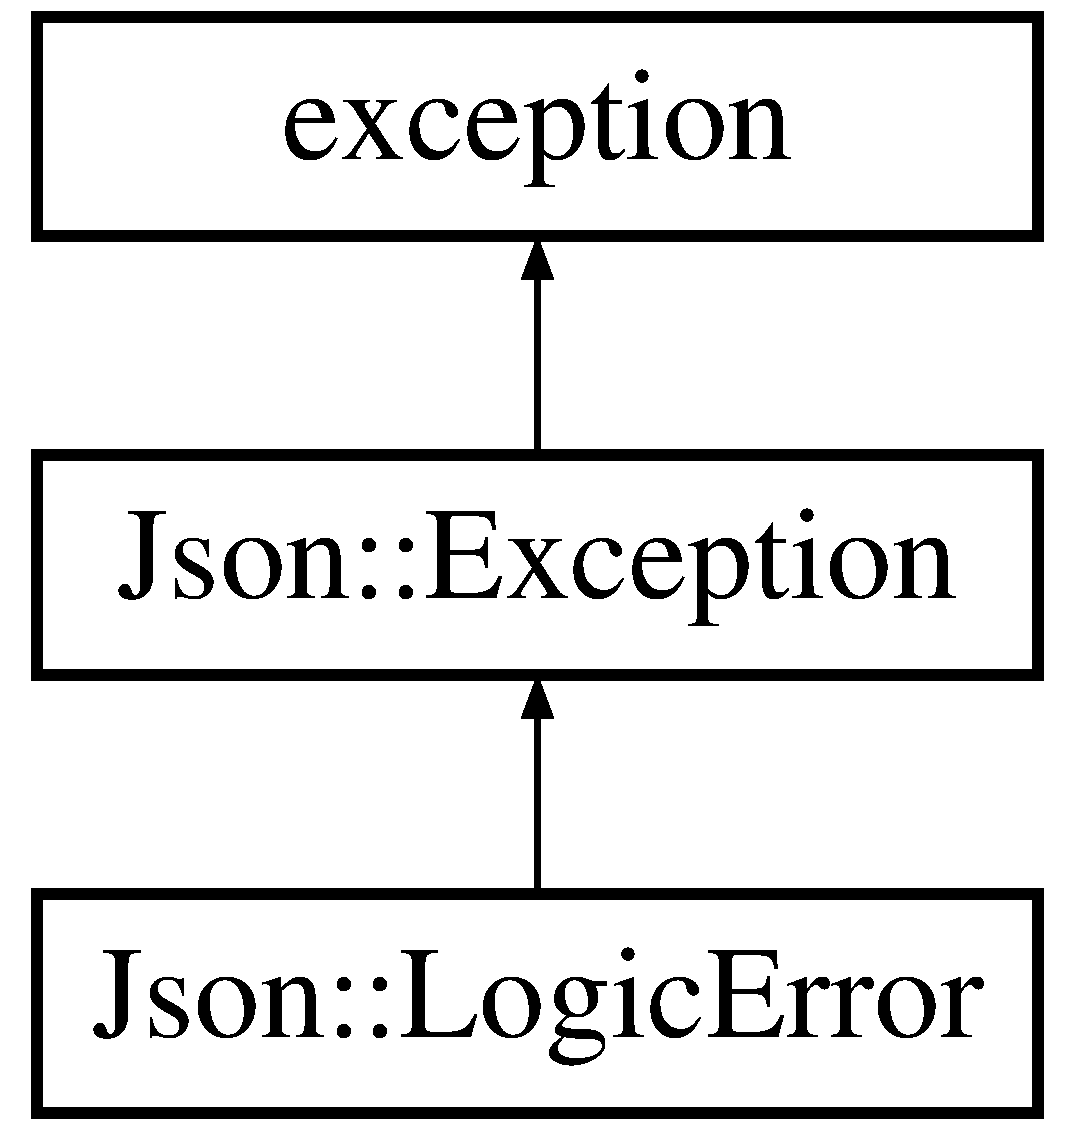
\includegraphics[height=3.000000cm]{classJson_1_1LogicError}
\end{center}
\end{figure}
\subsection*{Public Member Functions}
\begin{DoxyCompactItemize}
\item 
\mbox{\Hypertarget{classJson_1_1LogicError_acca679aa49768a4a1de7b705c67c2919}\label{classJson_1_1LogicError_acca679aa49768a4a1de7b705c67c2919}} 
{\bfseries Logic\+Error} (J\+S\+O\+N\+C\+P\+P\+\_\+\+S\+T\+R\+I\+NG const \&msg)
\end{DoxyCompactItemize}
\subsection*{Additional Inherited Members}


\subsection{Detailed Description}
Exceptions thrown by J\+S\+O\+N\+\_\+\+A\+S\+S\+E\+R\+T/\+J\+S\+O\+N\+\_\+\+F\+A\+IL macros.

These are precondition-\/violations (user bugs) and internal errors (our bugs).

\begin{DoxyRemark}{Remarks}
derived from \hyperlink{classJson_1_1Exception}{Json\+::\+Exception} 
\end{DoxyRemark}


The documentation for this class was generated from the following files\+:\begin{DoxyCompactItemize}
\item 
json/json.\+h\item 
jsoncpp.\+cpp\end{DoxyCompactItemize}

\hypertarget{classTBT_1_1Manager}{}\section{T\+BT\+:\+:Manager Class Reference}
\label{classTBT_1_1Manager}\index{T\+B\+T\+::\+Manager@{T\+B\+T\+::\+Manager}}
\subsection*{Public Member Functions}
\begin{DoxyCompactItemize}
\item 
\mbox{\Hypertarget{classTBT_1_1Manager_a04d5ae5069f1f17ee682f4ae68141687}\label{classTBT_1_1Manager_a04d5ae5069f1f17ee682f4ae68141687}} 
\hyperlink{classTBT_1_1Decoder}{Decoder} $\ast$ {\bfseries find\+Decoder} (uint16\+\_\+t dcc\+Address)
\item 
\mbox{\Hypertarget{classTBT_1_1Manager_a7b20f8a47d78cfd39649722a9fba2f7c}\label{classTBT_1_1Manager_a7b20f8a47d78cfd39649722a9fba2f7c}} 
void {\bfseries register\+Decoder} (\hyperlink{classTBT_1_1Decoder}{Decoder} $\ast$p\+Decoder)
\item 
\mbox{\Hypertarget{classTBT_1_1Manager_a507ac74f4adfbb6173728bebe71e40e6}\label{classTBT_1_1Manager_a507ac74f4adfbb6173728bebe71e40e6}} 
void {\bfseries unregister\+Decoder} (\hyperlink{classTBT_1_1Decoder}{Decoder} $\ast$p\+Decoder)
\item 
\mbox{\Hypertarget{classTBT_1_1Manager_aaac6dc1a57d9c578a3da2243584a8a22}\label{classTBT_1_1Manager_aaac6dc1a57d9c578a3da2243584a8a22}} 
void {\bfseries broadcast\+Loc\+Info\+Changed} (\hyperlink{classTBT_1_1LocDecoder}{Loc\+Decoder} $\ast$p\+Loc)
\item 
\mbox{\Hypertarget{classTBT_1_1Manager_a6e7616a839a1b48d89355bc740ed7793}\label{classTBT_1_1Manager_a6e7616a839a1b48d89355bc740ed7793}} 
void {\bfseries set\+Power\+State} (Power\+State new\+State)
\item 
\mbox{\Hypertarget{classTBT_1_1Manager_a5f5fdba7ccae731f3f348b572fd0ed16}\label{classTBT_1_1Manager_a5f5fdba7ccae731f3f348b572fd0ed16}} 
void {\bfseries set\+Emergency\+Stop} ()
\item 
\mbox{\Hypertarget{classTBT_1_1Manager_a007018b4e6441c9af63cb72f1ffc8a19}\label{classTBT_1_1Manager_a007018b4e6441c9af63cb72f1ffc8a19}} 
void {\bfseries get\+System\+State} (\hyperlink{structTBT_1_1SystemState}{System\+State} $\ast$p\+Msg)
\item 
\mbox{\Hypertarget{classTBT_1_1Manager_a78e5bea49f6662b5f44c1c0aafe4cb75}\label{classTBT_1_1Manager_a78e5bea49f6662b5f44c1c0aafe4cb75}} 
const uint8\+\_\+t \& {\bfseries get\+Central\+State} (void)
\end{DoxyCompactItemize}


The documentation for this class was generated from the following files\+:\begin{DoxyCompactItemize}
\item 
Manager.\+h\item 
Manager.\+cpp\end{DoxyCompactItemize}

\hypertarget{structmbuf}{}\section{mbuf Struct Reference}
\label{structmbuf}\index{mbuf@{mbuf}}
\subsection*{Public Attributes}
\begin{DoxyCompactItemize}
\item 
\mbox{\Hypertarget{structmbuf_ae2a6e23a4997e9aea0908628db2b23d0}\label{structmbuf_ae2a6e23a4997e9aea0908628db2b23d0}} 
char $\ast$ {\bfseries buf}
\item 
\mbox{\Hypertarget{structmbuf_a4da00860609dd46fe8b679d5e1deeac3}\label{structmbuf_a4da00860609dd46fe8b679d5e1deeac3}} 
size\+\_\+t {\bfseries len}
\item 
\mbox{\Hypertarget{structmbuf_ae245d03a50c2891c1fb228093d842270}\label{structmbuf_ae245d03a50c2891c1fb228093d842270}} 
size\+\_\+t {\bfseries size}
\end{DoxyCompactItemize}


The documentation for this struct was generated from the following file\+:\begin{DoxyCompactItemize}
\item 
mongoose.\+h\end{DoxyCompactItemize}

\hypertarget{structmg__add__sock__opts}{}\section{mg\+\_\+add\+\_\+sock\+\_\+opts Struct Reference}
\label{structmg__add__sock__opts}\index{mg\+\_\+add\+\_\+sock\+\_\+opts@{mg\+\_\+add\+\_\+sock\+\_\+opts}}
\subsection*{Public Attributes}
\begin{DoxyCompactItemize}
\item 
\mbox{\Hypertarget{structmg__add__sock__opts_af927a96c42e76f43592b510eca4e1f8e}\label{structmg__add__sock__opts_af927a96c42e76f43592b510eca4e1f8e}} 
void $\ast$ {\bfseries user\+\_\+data}
\item 
\mbox{\Hypertarget{structmg__add__sock__opts_ac836b917617be7c0a38e6a322cdf9cff}\label{structmg__add__sock__opts_ac836b917617be7c0a38e6a322cdf9cff}} 
unsigned int {\bfseries flags}
\item 
\mbox{\Hypertarget{structmg__add__sock__opts_a13c0a3d7dc05ad3873a03a7236735a50}\label{structmg__add__sock__opts_a13c0a3d7dc05ad3873a03a7236735a50}} 
const char $\ast$$\ast$ {\bfseries error\+\_\+string}
\item 
\mbox{\Hypertarget{structmg__add__sock__opts_a3d5516f6481c9a317b4708ec370a9b43}\label{structmg__add__sock__opts_a3d5516f6481c9a317b4708ec370a9b43}} 
struct \hyperlink{structmg__iface}{mg\+\_\+iface} $\ast$ {\bfseries iface}
\end{DoxyCompactItemize}


The documentation for this struct was generated from the following file\+:\begin{DoxyCompactItemize}
\item 
mongoose.\+h\end{DoxyCompactItemize}

\hypertarget{structmg__bind__opts}{}\section{mg\+\_\+bind\+\_\+opts Struct Reference}
\label{structmg__bind__opts}\index{mg\+\_\+bind\+\_\+opts@{mg\+\_\+bind\+\_\+opts}}


{\ttfamily \#include $<$mongoose.\+h$>$}

\subsection*{Public Attributes}
\begin{DoxyCompactItemize}
\item 
void $\ast$ \hyperlink{structmg__bind__opts_a3bd493ef5bd6c8da605b1480a6c189c4_a3bd493ef5bd6c8da605b1480a6c189c4}{user\+\_\+data}
\item 
unsigned int \hyperlink{structmg__bind__opts_ae257fe726a23692a36fb8c92885d4873_ae257fe726a23692a36fb8c92885d4873}{flags}
\item 
const char $\ast$$\ast$ \hyperlink{structmg__bind__opts_a9320251e7b1a273fedc123a3739fb9fa_a9320251e7b1a273fedc123a3739fb9fa}{error\+\_\+string}
\item 
struct \hyperlink{structmg__iface}{mg\+\_\+iface} $\ast$ \hyperlink{structmg__bind__opts_a328924ea266e19c9add95902d82271ad_a328924ea266e19c9add95902d82271ad}{iface}
\end{DoxyCompactItemize}


\subsection{Member Data Documentation}
\mbox{\Hypertarget{structmg__bind__opts_a9320251e7b1a273fedc123a3739fb9fa_a9320251e7b1a273fedc123a3739fb9fa}\label{structmg__bind__opts_a9320251e7b1a273fedc123a3739fb9fa_a9320251e7b1a273fedc123a3739fb9fa}} 
\index{mg\+\_\+bind\+\_\+opts@{mg\+\_\+bind\+\_\+opts}!error\+\_\+string@{error\+\_\+string}}
\index{error\+\_\+string@{error\+\_\+string}!mg\+\_\+bind\+\_\+opts@{mg\+\_\+bind\+\_\+opts}}
\subsubsection{\texorpdfstring{error\+\_\+string}{error\_string}}
{\footnotesize\ttfamily const char$\ast$$\ast$ mg\+\_\+bind\+\_\+opts\+::error\+\_\+string}



Referenced by mg\+\_\+bind\+\_\+opt().

\mbox{\Hypertarget{structmg__bind__opts_ae257fe726a23692a36fb8c92885d4873_ae257fe726a23692a36fb8c92885d4873}\label{structmg__bind__opts_ae257fe726a23692a36fb8c92885d4873_ae257fe726a23692a36fb8c92885d4873}} 
\index{mg\+\_\+bind\+\_\+opts@{mg\+\_\+bind\+\_\+opts}!flags@{flags}}
\index{flags@{flags}!mg\+\_\+bind\+\_\+opts@{mg\+\_\+bind\+\_\+opts}}
\subsubsection{\texorpdfstring{flags}{flags}}
{\footnotesize\ttfamily unsigned int mg\+\_\+bind\+\_\+opts\+::flags}

\mbox{\Hypertarget{structmg__bind__opts_a328924ea266e19c9add95902d82271ad_a328924ea266e19c9add95902d82271ad}\label{structmg__bind__opts_a328924ea266e19c9add95902d82271ad_a328924ea266e19c9add95902d82271ad}} 
\index{mg\+\_\+bind\+\_\+opts@{mg\+\_\+bind\+\_\+opts}!iface@{iface}}
\index{iface@{iface}!mg\+\_\+bind\+\_\+opts@{mg\+\_\+bind\+\_\+opts}}
\subsubsection{\texorpdfstring{iface}{iface}}
{\footnotesize\ttfamily struct \hyperlink{structmg__iface}{mg\+\_\+iface}$\ast$ mg\+\_\+bind\+\_\+opts\+::iface}



Referenced by mg\+\_\+tun\+\_\+do\+\_\+bind().

\mbox{\Hypertarget{structmg__bind__opts_a3bd493ef5bd6c8da605b1480a6c189c4_a3bd493ef5bd6c8da605b1480a6c189c4}\label{structmg__bind__opts_a3bd493ef5bd6c8da605b1480a6c189c4_a3bd493ef5bd6c8da605b1480a6c189c4}} 
\index{mg\+\_\+bind\+\_\+opts@{mg\+\_\+bind\+\_\+opts}!user\+\_\+data@{user\+\_\+data}}
\index{user\+\_\+data@{user\+\_\+data}!mg\+\_\+bind\+\_\+opts@{mg\+\_\+bind\+\_\+opts}}
\subsubsection{\texorpdfstring{user\+\_\+data}{user\_data}}
{\footnotesize\ttfamily void$\ast$ mg\+\_\+bind\+\_\+opts\+::user\+\_\+data}



Referenced by mg\+\_\+bind\+\_\+opt().



The documentation for this struct was generated from the following file\+:\begin{DoxyCompactItemize}
\item 
\hyperlink{mongoose_8h}{mongoose.\+h}\end{DoxyCompactItemize}

\hypertarget{structmg__connect__opts}{}\section{mg\+\_\+connect\+\_\+opts Struct Reference}
\label{structmg__connect__opts}\index{mg\+\_\+connect\+\_\+opts@{mg\+\_\+connect\+\_\+opts}}


{\ttfamily \#include $<$mongoose.\+h$>$}

\subsection*{Public Attributes}
\begin{DoxyCompactItemize}
\item 
void $\ast$ \hyperlink{structmg__connect__opts_a88039c409267c457638a0ebce97d7c5c_a88039c409267c457638a0ebce97d7c5c}{user\+\_\+data}
\item 
unsigned int \hyperlink{structmg__connect__opts_a794f93a8213aa29cdb59fb42075c0ab0_a794f93a8213aa29cdb59fb42075c0ab0}{flags}
\item 
const char $\ast$$\ast$ \hyperlink{structmg__connect__opts_a24fa9723e785487ed74b779c1e30ce75_a24fa9723e785487ed74b779c1e30ce75}{error\+\_\+string}
\item 
struct \hyperlink{structmg__iface}{mg\+\_\+iface} $\ast$ \hyperlink{structmg__connect__opts_a47c10391acd986fe2ff3f4f308bd1637_a47c10391acd986fe2ff3f4f308bd1637}{iface}
\item 
const char $\ast$ \hyperlink{structmg__connect__opts_a53edbf692c49f5ee86d2fe27ebba816c_a53edbf692c49f5ee86d2fe27ebba816c}{nameserver}
\end{DoxyCompactItemize}


\subsection{Member Data Documentation}
\mbox{\Hypertarget{structmg__connect__opts_a24fa9723e785487ed74b779c1e30ce75_a24fa9723e785487ed74b779c1e30ce75}\label{structmg__connect__opts_a24fa9723e785487ed74b779c1e30ce75_a24fa9723e785487ed74b779c1e30ce75}} 
\index{mg\+\_\+connect\+\_\+opts@{mg\+\_\+connect\+\_\+opts}!error\+\_\+string@{error\+\_\+string}}
\index{error\+\_\+string@{error\+\_\+string}!mg\+\_\+connect\+\_\+opts@{mg\+\_\+connect\+\_\+opts}}
\subsubsection{\texorpdfstring{error\+\_\+string}{error\_string}}
{\footnotesize\ttfamily const char$\ast$$\ast$ mg\+\_\+connect\+\_\+opts\+::error\+\_\+string}



Referenced by mg\+\_\+connect\+\_\+http\+\_\+base(), mg\+\_\+connect\+\_\+opt(), and mg\+\_\+parse\+\_\+http\+\_\+basic\+\_\+auth().

\mbox{\Hypertarget{structmg__connect__opts_a794f93a8213aa29cdb59fb42075c0ab0_a794f93a8213aa29cdb59fb42075c0ab0}\label{structmg__connect__opts_a794f93a8213aa29cdb59fb42075c0ab0_a794f93a8213aa29cdb59fb42075c0ab0}} 
\index{mg\+\_\+connect\+\_\+opts@{mg\+\_\+connect\+\_\+opts}!flags@{flags}}
\index{flags@{flags}!mg\+\_\+connect\+\_\+opts@{mg\+\_\+connect\+\_\+opts}}
\subsubsection{\texorpdfstring{flags}{flags}}
{\footnotesize\ttfamily unsigned int mg\+\_\+connect\+\_\+opts\+::flags}



Referenced by mg\+\_\+connect\+\_\+opt().

\mbox{\Hypertarget{structmg__connect__opts_a47c10391acd986fe2ff3f4f308bd1637_a47c10391acd986fe2ff3f4f308bd1637}\label{structmg__connect__opts_a47c10391acd986fe2ff3f4f308bd1637_a47c10391acd986fe2ff3f4f308bd1637}} 
\index{mg\+\_\+connect\+\_\+opts@{mg\+\_\+connect\+\_\+opts}!iface@{iface}}
\index{iface@{iface}!mg\+\_\+connect\+\_\+opts@{mg\+\_\+connect\+\_\+opts}}
\subsubsection{\texorpdfstring{iface}{iface}}
{\footnotesize\ttfamily struct \hyperlink{structmg__iface}{mg\+\_\+iface}$\ast$ mg\+\_\+connect\+\_\+opts\+::iface}

\mbox{\Hypertarget{structmg__connect__opts_a53edbf692c49f5ee86d2fe27ebba816c_a53edbf692c49f5ee86d2fe27ebba816c}\label{structmg__connect__opts_a53edbf692c49f5ee86d2fe27ebba816c_a53edbf692c49f5ee86d2fe27ebba816c}} 
\index{mg\+\_\+connect\+\_\+opts@{mg\+\_\+connect\+\_\+opts}!nameserver@{nameserver}}
\index{nameserver@{nameserver}!mg\+\_\+connect\+\_\+opts@{mg\+\_\+connect\+\_\+opts}}
\subsubsection{\texorpdfstring{nameserver}{nameserver}}
{\footnotesize\ttfamily const char$\ast$ mg\+\_\+connect\+\_\+opts\+::nameserver}



Referenced by mg\+\_\+connect\+\_\+opt().

\mbox{\Hypertarget{structmg__connect__opts_a88039c409267c457638a0ebce97d7c5c_a88039c409267c457638a0ebce97d7c5c}\label{structmg__connect__opts_a88039c409267c457638a0ebce97d7c5c_a88039c409267c457638a0ebce97d7c5c}} 
\index{mg\+\_\+connect\+\_\+opts@{mg\+\_\+connect\+\_\+opts}!user\+\_\+data@{user\+\_\+data}}
\index{user\+\_\+data@{user\+\_\+data}!mg\+\_\+connect\+\_\+opts@{mg\+\_\+connect\+\_\+opts}}
\subsubsection{\texorpdfstring{user\+\_\+data}{user\_data}}
{\footnotesize\ttfamily void$\ast$ mg\+\_\+connect\+\_\+opts\+::user\+\_\+data}



Referenced by mg\+\_\+connect\+\_\+opt().



The documentation for this struct was generated from the following file\+:\begin{DoxyCompactItemize}
\item 
\hyperlink{mongoose_8h}{mongoose.\+h}\end{DoxyCompactItemize}

\hypertarget{structmg__connection}{}\section{mg\+\_\+connection Struct Reference}
\label{structmg__connection}\index{mg\+\_\+connection@{mg\+\_\+connection}}
\subsection*{Public Attributes}
\begin{DoxyCompactItemize}
\item 
\mbox{\Hypertarget{structmg__connection_afcfd89f119a87cba6f6dfec2d2eda5d9}\label{structmg__connection_afcfd89f119a87cba6f6dfec2d2eda5d9}} 
struct \hyperlink{structmg__connection}{mg\+\_\+connection} $\ast$ {\bfseries next}
\item 
\mbox{\Hypertarget{structmg__connection_aa93fd5ca83f11230bc971a68a7fa8d5e}\label{structmg__connection_aa93fd5ca83f11230bc971a68a7fa8d5e}} 
struct \hyperlink{structmg__connection}{mg\+\_\+connection} $\ast$ {\bfseries prev}
\item 
\mbox{\Hypertarget{structmg__connection_a9392bec67d0dc8df58e6c171214ddf8d}\label{structmg__connection_a9392bec67d0dc8df58e6c171214ddf8d}} 
struct \hyperlink{structmg__connection}{mg\+\_\+connection} $\ast$ {\bfseries listener}
\item 
\mbox{\Hypertarget{structmg__connection_ac341f1f2bd18e030fe90a914e4517506}\label{structmg__connection_ac341f1f2bd18e030fe90a914e4517506}} 
struct \hyperlink{structmg__mgr}{mg\+\_\+mgr} $\ast$ {\bfseries mgr}
\item 
\mbox{\Hypertarget{structmg__connection_a608f2461b3dd53e503d6ed3c84ec55b0}\label{structmg__connection_a608f2461b3dd53e503d6ed3c84ec55b0}} 
sock\+\_\+t {\bfseries sock}
\item 
\mbox{\Hypertarget{structmg__connection_aa13a0bd4a2ce3d6384866acb7e00344a}\label{structmg__connection_aa13a0bd4a2ce3d6384866acb7e00344a}} 
int {\bfseries err}
\item 
\mbox{\Hypertarget{structmg__connection_a3dfa1816f5a4b0725d9d04be75bbb3f8}\label{structmg__connection_a3dfa1816f5a4b0725d9d04be75bbb3f8}} 
union \hyperlink{unionsocket__address}{socket\+\_\+address} {\bfseries sa}
\item 
\mbox{\Hypertarget{structmg__connection_ab15e90e7fb7b8719cc7dcc67f45856e1}\label{structmg__connection_ab15e90e7fb7b8719cc7dcc67f45856e1}} 
size\+\_\+t {\bfseries recv\+\_\+mbuf\+\_\+limit}
\item 
\mbox{\Hypertarget{structmg__connection_a72adb9aba4bbe59a9bd591de496713b3}\label{structmg__connection_a72adb9aba4bbe59a9bd591de496713b3}} 
struct \hyperlink{structmbuf}{mbuf} {\bfseries recv\+\_\+mbuf}
\item 
\mbox{\Hypertarget{structmg__connection_a70076f5da9c9d01e77acb3547941671c}\label{structmg__connection_a70076f5da9c9d01e77acb3547941671c}} 
struct \hyperlink{structmbuf}{mbuf} {\bfseries send\+\_\+mbuf}
\item 
\mbox{\Hypertarget{structmg__connection_aaf0f39b26deef84e6c204a176ea1e50a}\label{structmg__connection_aaf0f39b26deef84e6c204a176ea1e50a}} 
time\+\_\+t {\bfseries last\+\_\+io\+\_\+time}
\item 
\mbox{\Hypertarget{structmg__connection_a84d1a7e42f1326c70f61f71e65082dc0}\label{structmg__connection_a84d1a7e42f1326c70f61f71e65082dc0}} 
double {\bfseries ev\+\_\+timer\+\_\+time}
\item 
\mbox{\Hypertarget{structmg__connection_ae6b1f0d002253c0f80371fc5a7bbfc70}\label{structmg__connection_ae6b1f0d002253c0f80371fc5a7bbfc70}} 
mg\+\_\+event\+\_\+handler\+\_\+t {\bfseries proto\+\_\+handler}
\item 
\mbox{\Hypertarget{structmg__connection_a7508851a3c070a1357c226781fa92bb7}\label{structmg__connection_a7508851a3c070a1357c226781fa92bb7}} 
void $\ast$ {\bfseries proto\+\_\+data}
\item 
\mbox{\Hypertarget{structmg__connection_a834e7757b28379b2ca0b8b6c51d7ba95}\label{structmg__connection_a834e7757b28379b2ca0b8b6c51d7ba95}} 
void($\ast$ {\bfseries proto\+\_\+data\+\_\+destructor} )(void $\ast$proto\+\_\+data)
\item 
\mbox{\Hypertarget{structmg__connection_a1f14bd154357c301cce137c9ac1d1edb}\label{structmg__connection_a1f14bd154357c301cce137c9ac1d1edb}} 
mg\+\_\+event\+\_\+handler\+\_\+t {\bfseries handler}
\item 
\mbox{\Hypertarget{structmg__connection_ab6d66a4eacc5d4d15f817ce98f26322d}\label{structmg__connection_ab6d66a4eacc5d4d15f817ce98f26322d}} 
void $\ast$ {\bfseries user\+\_\+data}
\item 
\mbox{\Hypertarget{structmg__connection_ad4386d39d9feedc547a1b1fcc8c5c7de}\label{structmg__connection_ad4386d39d9feedc547a1b1fcc8c5c7de}} 
\begin{tabbing}
xx\=xx\=xx\=xx\=xx\=xx\=xx\=xx\=xx\=\kill
union \{\\
\>void $\ast$ {\bfseries v}\\
\>mg\_event\_handler\_t {\bfseries f}\\
\} {\bfseries priv\_1}\\

\end{tabbing}\item 
\mbox{\Hypertarget{structmg__connection_aeb5efea496ac74ed2e0b8864f4fd6f65}\label{structmg__connection_aeb5efea496ac74ed2e0b8864f4fd6f65}} 
void $\ast$ {\bfseries priv\+\_\+2}
\item 
\mbox{\Hypertarget{structmg__connection_a19cb5ee4c2402582dcf4cb6a4f899136}\label{structmg__connection_a19cb5ee4c2402582dcf4cb6a4f899136}} 
void $\ast$ {\bfseries mgr\+\_\+data}
\item 
\mbox{\Hypertarget{structmg__connection_a6f337461553de516901473bd8bb11a0a}\label{structmg__connection_a6f337461553de516901473bd8bb11a0a}} 
struct \hyperlink{structmg__iface}{mg\+\_\+iface} $\ast$ {\bfseries iface}
\item 
\mbox{\Hypertarget{structmg__connection_aa47edda11152dd7769a76d806a87e1aa}\label{structmg__connection_aa47edda11152dd7769a76d806a87e1aa}} 
unsigned long {\bfseries flags}
\end{DoxyCompactItemize}


The documentation for this struct was generated from the following file\+:\begin{DoxyCompactItemize}
\item 
mongoose.\+h\end{DoxyCompactItemize}

\hypertarget{structmg__dns__header}{}\section{mg\+\_\+dns\+\_\+header Struct Reference}
\label{structmg__dns__header}\index{mg\+\_\+dns\+\_\+header@{mg\+\_\+dns\+\_\+header}}
\subsection*{Public Attributes}
\begin{DoxyCompactItemize}
\item 
uint16\+\_\+t \hyperlink{structmg__dns__header_a00963ebb1d83de6f48f7733679c4b8a7_a00963ebb1d83de6f48f7733679c4b8a7}{transaction\+\_\+id}
\item 
uint16\+\_\+t \hyperlink{structmg__dns__header_a42a3a0530dcceaa67b96f054c1c44aa6_a42a3a0530dcceaa67b96f054c1c44aa6}{flags}
\item 
uint16\+\_\+t \hyperlink{structmg__dns__header_a156d3f5926d1fdb24bcbcba1f273c59a_a156d3f5926d1fdb24bcbcba1f273c59a}{num\+\_\+questions}
\item 
uint16\+\_\+t \hyperlink{structmg__dns__header_a2d577357775702ca340492ca51379b21_a2d577357775702ca340492ca51379b21}{num\+\_\+answers}
\item 
uint16\+\_\+t \hyperlink{structmg__dns__header_a90a7621286acf1c8b78d3ee450dce9b6_a90a7621286acf1c8b78d3ee450dce9b6}{num\+\_\+authority\+\_\+prs}
\item 
uint16\+\_\+t \hyperlink{structmg__dns__header_aed8714aa60f2cc79dc0c81378c2ddb50_aed8714aa60f2cc79dc0c81378c2ddb50}{num\+\_\+other\+\_\+prs}
\end{DoxyCompactItemize}


\subsection{Member Data Documentation}
\mbox{\Hypertarget{structmg__dns__header_a42a3a0530dcceaa67b96f054c1c44aa6_a42a3a0530dcceaa67b96f054c1c44aa6}\label{structmg__dns__header_a42a3a0530dcceaa67b96f054c1c44aa6_a42a3a0530dcceaa67b96f054c1c44aa6}} 
\index{mg\+\_\+dns\+\_\+header@{mg\+\_\+dns\+\_\+header}!flags@{flags}}
\index{flags@{flags}!mg\+\_\+dns\+\_\+header@{mg\+\_\+dns\+\_\+header}}
\subsubsection{\texorpdfstring{flags}{flags}}
{\footnotesize\ttfamily uint16\+\_\+t mg\+\_\+dns\+\_\+header\+::flags}



Referenced by mg\+\_\+dns\+\_\+insert\+\_\+header(), and mg\+\_\+parse\+\_\+dns().

\mbox{\Hypertarget{structmg__dns__header_a2d577357775702ca340492ca51379b21_a2d577357775702ca340492ca51379b21}\label{structmg__dns__header_a2d577357775702ca340492ca51379b21_a2d577357775702ca340492ca51379b21}} 
\index{mg\+\_\+dns\+\_\+header@{mg\+\_\+dns\+\_\+header}!num\+\_\+answers@{num\+\_\+answers}}
\index{num\+\_\+answers@{num\+\_\+answers}!mg\+\_\+dns\+\_\+header@{mg\+\_\+dns\+\_\+header}}
\subsubsection{\texorpdfstring{num\+\_\+answers}{num\_answers}}
{\footnotesize\ttfamily uint16\+\_\+t mg\+\_\+dns\+\_\+header\+::num\+\_\+answers}



Referenced by mg\+\_\+dns\+\_\+insert\+\_\+header(), and mg\+\_\+parse\+\_\+dns().

\mbox{\Hypertarget{structmg__dns__header_a90a7621286acf1c8b78d3ee450dce9b6_a90a7621286acf1c8b78d3ee450dce9b6}\label{structmg__dns__header_a90a7621286acf1c8b78d3ee450dce9b6_a90a7621286acf1c8b78d3ee450dce9b6}} 
\index{mg\+\_\+dns\+\_\+header@{mg\+\_\+dns\+\_\+header}!num\+\_\+authority\+\_\+prs@{num\+\_\+authority\+\_\+prs}}
\index{num\+\_\+authority\+\_\+prs@{num\+\_\+authority\+\_\+prs}!mg\+\_\+dns\+\_\+header@{mg\+\_\+dns\+\_\+header}}
\subsubsection{\texorpdfstring{num\+\_\+authority\+\_\+prs}{num\_authority\_prs}}
{\footnotesize\ttfamily uint16\+\_\+t mg\+\_\+dns\+\_\+header\+::num\+\_\+authority\+\_\+prs}

\mbox{\Hypertarget{structmg__dns__header_aed8714aa60f2cc79dc0c81378c2ddb50_aed8714aa60f2cc79dc0c81378c2ddb50}\label{structmg__dns__header_aed8714aa60f2cc79dc0c81378c2ddb50_aed8714aa60f2cc79dc0c81378c2ddb50}} 
\index{mg\+\_\+dns\+\_\+header@{mg\+\_\+dns\+\_\+header}!num\+\_\+other\+\_\+prs@{num\+\_\+other\+\_\+prs}}
\index{num\+\_\+other\+\_\+prs@{num\+\_\+other\+\_\+prs}!mg\+\_\+dns\+\_\+header@{mg\+\_\+dns\+\_\+header}}
\subsubsection{\texorpdfstring{num\+\_\+other\+\_\+prs}{num\_other\_prs}}
{\footnotesize\ttfamily uint16\+\_\+t mg\+\_\+dns\+\_\+header\+::num\+\_\+other\+\_\+prs}

\mbox{\Hypertarget{structmg__dns__header_a156d3f5926d1fdb24bcbcba1f273c59a_a156d3f5926d1fdb24bcbcba1f273c59a}\label{structmg__dns__header_a156d3f5926d1fdb24bcbcba1f273c59a_a156d3f5926d1fdb24bcbcba1f273c59a}} 
\index{mg\+\_\+dns\+\_\+header@{mg\+\_\+dns\+\_\+header}!num\+\_\+questions@{num\+\_\+questions}}
\index{num\+\_\+questions@{num\+\_\+questions}!mg\+\_\+dns\+\_\+header@{mg\+\_\+dns\+\_\+header}}
\subsubsection{\texorpdfstring{num\+\_\+questions}{num\_questions}}
{\footnotesize\ttfamily uint16\+\_\+t mg\+\_\+dns\+\_\+header\+::num\+\_\+questions}



Referenced by mg\+\_\+dns\+\_\+insert\+\_\+header(), and mg\+\_\+parse\+\_\+dns().

\mbox{\Hypertarget{structmg__dns__header_a00963ebb1d83de6f48f7733679c4b8a7_a00963ebb1d83de6f48f7733679c4b8a7}\label{structmg__dns__header_a00963ebb1d83de6f48f7733679c4b8a7_a00963ebb1d83de6f48f7733679c4b8a7}} 
\index{mg\+\_\+dns\+\_\+header@{mg\+\_\+dns\+\_\+header}!transaction\+\_\+id@{transaction\+\_\+id}}
\index{transaction\+\_\+id@{transaction\+\_\+id}!mg\+\_\+dns\+\_\+header@{mg\+\_\+dns\+\_\+header}}
\subsubsection{\texorpdfstring{transaction\+\_\+id}{transaction\_id}}
{\footnotesize\ttfamily uint16\+\_\+t mg\+\_\+dns\+\_\+header\+::transaction\+\_\+id}



Referenced by mg\+\_\+dns\+\_\+insert\+\_\+header(), and mg\+\_\+parse\+\_\+dns().



The documentation for this struct was generated from the following file\+:\begin{DoxyCompactItemize}
\item 
\hyperlink{mongoose_8c}{mongoose.\+c}\end{DoxyCompactItemize}

\hypertarget{structmg__dns__message}{}\section{mg\+\_\+dns\+\_\+message Struct Reference}
\label{structmg__dns__message}\index{mg\+\_\+dns\+\_\+message@{mg\+\_\+dns\+\_\+message}}


{\ttfamily \#include $<$mongoose.\+h$>$}

\subsection*{Public Attributes}
\begin{DoxyCompactItemize}
\item 
struct \hyperlink{structmg__str}{mg\+\_\+str} \hyperlink{structmg__dns__message_ae8543b2a3044c785b4bf0dc4fc39beff_ae8543b2a3044c785b4bf0dc4fc39beff}{pkt}
\item 
uint16\+\_\+t \hyperlink{structmg__dns__message_a87f916bb55651d46ce74f930a5e08327_a87f916bb55651d46ce74f930a5e08327}{flags}
\item 
uint16\+\_\+t \hyperlink{structmg__dns__message_afb4a01337779347f74a214c7a273ebcb_afb4a01337779347f74a214c7a273ebcb}{transaction\+\_\+id}
\item 
int \hyperlink{structmg__dns__message_a035ced22ef43b6b23ad6df3ad3aad126_a035ced22ef43b6b23ad6df3ad3aad126}{num\+\_\+questions}
\item 
int \hyperlink{structmg__dns__message_a6ebecefbdcb5c292f439123b7c780517_a6ebecefbdcb5c292f439123b7c780517}{num\+\_\+answers}
\item 
struct \hyperlink{structmg__dns__resource__record}{mg\+\_\+dns\+\_\+resource\+\_\+record} \hyperlink{structmg__dns__message_a866a83825f2daa4043aa20acded4f007_a866a83825f2daa4043aa20acded4f007}{questions} \mbox{[}\hyperlink{mongoose_8h_a84f36ff9caf50e0d70d10244a2c64b45_a84f36ff9caf50e0d70d10244a2c64b45}{M\+G\+\_\+\+M\+A\+X\+\_\+\+D\+N\+S\+\_\+\+Q\+U\+E\+S\+T\+I\+O\+NS}\mbox{]}
\item 
struct \hyperlink{structmg__dns__resource__record}{mg\+\_\+dns\+\_\+resource\+\_\+record} \hyperlink{structmg__dns__message_a76e7c9d2d5f7f621df2d2551f0163e01_a76e7c9d2d5f7f621df2d2551f0163e01}{answers} \mbox{[}\hyperlink{mongoose_8h_a1832d47a93efb88b807286ed1ae80646_a1832d47a93efb88b807286ed1ae80646}{M\+G\+\_\+\+M\+A\+X\+\_\+\+D\+N\+S\+\_\+\+A\+N\+S\+W\+E\+RS}\mbox{]}
\end{DoxyCompactItemize}


\subsection{Member Data Documentation}
\mbox{\Hypertarget{structmg__dns__message_a76e7c9d2d5f7f621df2d2551f0163e01_a76e7c9d2d5f7f621df2d2551f0163e01}\label{structmg__dns__message_a76e7c9d2d5f7f621df2d2551f0163e01_a76e7c9d2d5f7f621df2d2551f0163e01}} 
\index{mg\+\_\+dns\+\_\+message@{mg\+\_\+dns\+\_\+message}!answers@{answers}}
\index{answers@{answers}!mg\+\_\+dns\+\_\+message@{mg\+\_\+dns\+\_\+message}}
\subsubsection{\texorpdfstring{answers}{answers}}
{\footnotesize\ttfamily struct \hyperlink{structmg__dns__resource__record}{mg\+\_\+dns\+\_\+resource\+\_\+record} mg\+\_\+dns\+\_\+message\+::answers\mbox{[}\hyperlink{mongoose_8h_a1832d47a93efb88b807286ed1ae80646_a1832d47a93efb88b807286ed1ae80646}{M\+G\+\_\+\+M\+A\+X\+\_\+\+D\+N\+S\+\_\+\+A\+N\+S\+W\+E\+RS}\mbox{]}}



Referenced by mg\+\_\+dns\+\_\+next\+\_\+record(), mg\+\_\+parse\+\_\+dns(), mg\+\_\+set\+\_\+protocol\+\_\+dns(), and resolve\+\_\+cb().

\mbox{\Hypertarget{structmg__dns__message_a87f916bb55651d46ce74f930a5e08327_a87f916bb55651d46ce74f930a5e08327}\label{structmg__dns__message_a87f916bb55651d46ce74f930a5e08327_a87f916bb55651d46ce74f930a5e08327}} 
\index{mg\+\_\+dns\+\_\+message@{mg\+\_\+dns\+\_\+message}!flags@{flags}}
\index{flags@{flags}!mg\+\_\+dns\+\_\+message@{mg\+\_\+dns\+\_\+message}}
\subsubsection{\texorpdfstring{flags}{flags}}
{\footnotesize\ttfamily uint16\+\_\+t mg\+\_\+dns\+\_\+message\+::flags}



Referenced by dns\+\_\+handler(), mg\+\_\+dns\+\_\+insert\+\_\+header(), mg\+\_\+parse\+\_\+dns(), and mg\+\_\+send\+\_\+dns\+\_\+query().

\mbox{\Hypertarget{structmg__dns__message_a6ebecefbdcb5c292f439123b7c780517_a6ebecefbdcb5c292f439123b7c780517}\label{structmg__dns__message_a6ebecefbdcb5c292f439123b7c780517_a6ebecefbdcb5c292f439123b7c780517}} 
\index{mg\+\_\+dns\+\_\+message@{mg\+\_\+dns\+\_\+message}!num\+\_\+answers@{num\+\_\+answers}}
\index{num\+\_\+answers@{num\+\_\+answers}!mg\+\_\+dns\+\_\+message@{mg\+\_\+dns\+\_\+message}}
\subsubsection{\texorpdfstring{num\+\_\+answers}{num\_answers}}
{\footnotesize\ttfamily int mg\+\_\+dns\+\_\+message\+::num\+\_\+answers}



Referenced by mg\+\_\+dns\+\_\+insert\+\_\+header(), mg\+\_\+dns\+\_\+next\+\_\+record(), mg\+\_\+parse\+\_\+dns(), mg\+\_\+resolve\+\_\+async\+\_\+eh(), mg\+\_\+set\+\_\+protocol\+\_\+dns(), and resolve\+\_\+cb().

\mbox{\Hypertarget{structmg__dns__message_a035ced22ef43b6b23ad6df3ad3aad126_a035ced22ef43b6b23ad6df3ad3aad126}\label{structmg__dns__message_a035ced22ef43b6b23ad6df3ad3aad126_a035ced22ef43b6b23ad6df3ad3aad126}} 
\index{mg\+\_\+dns\+\_\+message@{mg\+\_\+dns\+\_\+message}!num\+\_\+questions@{num\+\_\+questions}}
\index{num\+\_\+questions@{num\+\_\+questions}!mg\+\_\+dns\+\_\+message@{mg\+\_\+dns\+\_\+message}}
\subsubsection{\texorpdfstring{num\+\_\+questions}{num\_questions}}
{\footnotesize\ttfamily int mg\+\_\+dns\+\_\+message\+::num\+\_\+questions}



Referenced by mg\+\_\+dns\+\_\+copy\+\_\+questions(), mg\+\_\+dns\+\_\+insert\+\_\+header(), mg\+\_\+parse\+\_\+dns(), and mg\+\_\+send\+\_\+dns\+\_\+query().

\mbox{\Hypertarget{structmg__dns__message_ae8543b2a3044c785b4bf0dc4fc39beff_ae8543b2a3044c785b4bf0dc4fc39beff}\label{structmg__dns__message_ae8543b2a3044c785b4bf0dc4fc39beff_ae8543b2a3044c785b4bf0dc4fc39beff}} 
\index{mg\+\_\+dns\+\_\+message@{mg\+\_\+dns\+\_\+message}!pkt@{pkt}}
\index{pkt@{pkt}!mg\+\_\+dns\+\_\+message@{mg\+\_\+dns\+\_\+message}}
\subsubsection{\texorpdfstring{pkt}{pkt}}
{\footnotesize\ttfamily struct \hyperlink{structmg__str}{mg\+\_\+str} mg\+\_\+dns\+\_\+message\+::pkt}



Referenced by mg\+\_\+dns\+\_\+copy\+\_\+questions(), mg\+\_\+dns\+\_\+parse\+\_\+record\+\_\+data(), mg\+\_\+dns\+\_\+uncompress\+\_\+name(), and mg\+\_\+parse\+\_\+dns().

\mbox{\Hypertarget{structmg__dns__message_a866a83825f2daa4043aa20acded4f007_a866a83825f2daa4043aa20acded4f007}\label{structmg__dns__message_a866a83825f2daa4043aa20acded4f007_a866a83825f2daa4043aa20acded4f007}} 
\index{mg\+\_\+dns\+\_\+message@{mg\+\_\+dns\+\_\+message}!questions@{questions}}
\index{questions@{questions}!mg\+\_\+dns\+\_\+message@{mg\+\_\+dns\+\_\+message}}
\subsubsection{\texorpdfstring{questions}{questions}}
{\footnotesize\ttfamily struct \hyperlink{structmg__dns__resource__record}{mg\+\_\+dns\+\_\+resource\+\_\+record} mg\+\_\+dns\+\_\+message\+::questions\mbox{[}\hyperlink{mongoose_8h_a84f36ff9caf50e0d70d10244a2c64b45_a84f36ff9caf50e0d70d10244a2c64b45}{M\+G\+\_\+\+M\+A\+X\+\_\+\+D\+N\+S\+\_\+\+Q\+U\+E\+S\+T\+I\+O\+NS}\mbox{]}}



Referenced by mg\+\_\+dns\+\_\+copy\+\_\+questions(), mg\+\_\+parse\+\_\+dns(), and mg\+\_\+send\+\_\+dns\+\_\+query().

\mbox{\Hypertarget{structmg__dns__message_afb4a01337779347f74a214c7a273ebcb_afb4a01337779347f74a214c7a273ebcb}\label{structmg__dns__message_afb4a01337779347f74a214c7a273ebcb_afb4a01337779347f74a214c7a273ebcb}} 
\index{mg\+\_\+dns\+\_\+message@{mg\+\_\+dns\+\_\+message}!transaction\+\_\+id@{transaction\+\_\+id}}
\index{transaction\+\_\+id@{transaction\+\_\+id}!mg\+\_\+dns\+\_\+message@{mg\+\_\+dns\+\_\+message}}
\subsubsection{\texorpdfstring{transaction\+\_\+id}{transaction\_id}}
{\footnotesize\ttfamily uint16\+\_\+t mg\+\_\+dns\+\_\+message\+::transaction\+\_\+id}



Referenced by mg\+\_\+dns\+\_\+insert\+\_\+header(), mg\+\_\+parse\+\_\+dns(), and mg\+\_\+send\+\_\+dns\+\_\+query().



The documentation for this struct was generated from the following file\+:\begin{DoxyCompactItemize}
\item 
\hyperlink{mongoose_8h}{mongoose.\+h}\end{DoxyCompactItemize}

\hypertarget{structmg__dns__resource__record}{}\section{mg\+\_\+dns\+\_\+resource\+\_\+record Struct Reference}
\label{structmg__dns__resource__record}\index{mg\+\_\+dns\+\_\+resource\+\_\+record@{mg\+\_\+dns\+\_\+resource\+\_\+record}}


{\ttfamily \#include $<$mongoose.\+h$>$}

\subsection*{Public Attributes}
\begin{DoxyCompactItemize}
\item 
struct \hyperlink{structmg__str}{mg\+\_\+str} \hyperlink{structmg__dns__resource__record_afd27e187a02127a98a04757013aecd48_afd27e187a02127a98a04757013aecd48}{name}
\item 
int \hyperlink{structmg__dns__resource__record_a9d314632522fcca513858285c639bee9_a9d314632522fcca513858285c639bee9}{rtype}
\item 
int \hyperlink{structmg__dns__resource__record_a9be7dc2d7ef4e2dc20413289a55f6ff7_a9be7dc2d7ef4e2dc20413289a55f6ff7}{rclass}
\item 
int \hyperlink{structmg__dns__resource__record_aa5d1c1a7ba2d02908c27fab68ded25be_aa5d1c1a7ba2d02908c27fab68ded25be}{ttl}
\item 
enum \hyperlink{mongoose_8h_abc1e540c922be63eea4488f520e3523d_abc1e540c922be63eea4488f520e3523d}{mg\+\_\+dns\+\_\+resource\+\_\+record\+\_\+kind} \hyperlink{structmg__dns__resource__record_a6f9d5dda9d8ae9240a74282c44d4a555_a6f9d5dda9d8ae9240a74282c44d4a555}{kind}
\item 
struct \hyperlink{structmg__str}{mg\+\_\+str} \hyperlink{structmg__dns__resource__record_ac169801d0c9ce94137fcce9a3f629152_ac169801d0c9ce94137fcce9a3f629152}{rdata}
\end{DoxyCompactItemize}


\subsection{Member Data Documentation}
\mbox{\Hypertarget{structmg__dns__resource__record_a6f9d5dda9d8ae9240a74282c44d4a555_a6f9d5dda9d8ae9240a74282c44d4a555}\label{structmg__dns__resource__record_a6f9d5dda9d8ae9240a74282c44d4a555_a6f9d5dda9d8ae9240a74282c44d4a555}} 
\index{mg\+\_\+dns\+\_\+resource\+\_\+record@{mg\+\_\+dns\+\_\+resource\+\_\+record}!kind@{kind}}
\index{kind@{kind}!mg\+\_\+dns\+\_\+resource\+\_\+record@{mg\+\_\+dns\+\_\+resource\+\_\+record}}
\subsubsection{\texorpdfstring{kind}{kind}}
{\footnotesize\ttfamily enum \hyperlink{mongoose_8h_abc1e540c922be63eea4488f520e3523d_abc1e540c922be63eea4488f520e3523d}{mg\+\_\+dns\+\_\+resource\+\_\+record\+\_\+kind} mg\+\_\+dns\+\_\+resource\+\_\+record\+::kind}



Referenced by mg\+\_\+dns\+\_\+encode\+\_\+record(), mg\+\_\+parse\+\_\+dns\+\_\+resource\+\_\+record(), mg\+\_\+send\+\_\+dns\+\_\+query(), and mg\+\_\+set\+\_\+protocol\+\_\+dns().

\mbox{\Hypertarget{structmg__dns__resource__record_afd27e187a02127a98a04757013aecd48_afd27e187a02127a98a04757013aecd48}\label{structmg__dns__resource__record_afd27e187a02127a98a04757013aecd48_afd27e187a02127a98a04757013aecd48}} 
\index{mg\+\_\+dns\+\_\+resource\+\_\+record@{mg\+\_\+dns\+\_\+resource\+\_\+record}!name@{name}}
\index{name@{name}!mg\+\_\+dns\+\_\+resource\+\_\+record@{mg\+\_\+dns\+\_\+resource\+\_\+record}}
\subsubsection{\texorpdfstring{name}{name}}
{\footnotesize\ttfamily struct \hyperlink{structmg__str}{mg\+\_\+str} mg\+\_\+dns\+\_\+resource\+\_\+record\+::name}



Referenced by mg\+\_\+dns\+\_\+copy\+\_\+questions(), mg\+\_\+dns\+\_\+encode\+\_\+name(), mg\+\_\+parse\+\_\+dns\+\_\+resource\+\_\+record(), and mg\+\_\+set\+\_\+protocol\+\_\+dns().

\mbox{\Hypertarget{structmg__dns__resource__record_a9be7dc2d7ef4e2dc20413289a55f6ff7_a9be7dc2d7ef4e2dc20413289a55f6ff7}\label{structmg__dns__resource__record_a9be7dc2d7ef4e2dc20413289a55f6ff7_a9be7dc2d7ef4e2dc20413289a55f6ff7}} 
\index{mg\+\_\+dns\+\_\+resource\+\_\+record@{mg\+\_\+dns\+\_\+resource\+\_\+record}!rclass@{rclass}}
\index{rclass@{rclass}!mg\+\_\+dns\+\_\+resource\+\_\+record@{mg\+\_\+dns\+\_\+resource\+\_\+record}}
\subsubsection{\texorpdfstring{rclass}{rclass}}
{\footnotesize\ttfamily int mg\+\_\+dns\+\_\+resource\+\_\+record\+::rclass}



Referenced by mg\+\_\+dns\+\_\+encode\+\_\+record(), mg\+\_\+parse\+\_\+dns\+\_\+resource\+\_\+record(), and mg\+\_\+send\+\_\+dns\+\_\+query().

\mbox{\Hypertarget{structmg__dns__resource__record_ac169801d0c9ce94137fcce9a3f629152_ac169801d0c9ce94137fcce9a3f629152}\label{structmg__dns__resource__record_ac169801d0c9ce94137fcce9a3f629152_ac169801d0c9ce94137fcce9a3f629152}} 
\index{mg\+\_\+dns\+\_\+resource\+\_\+record@{mg\+\_\+dns\+\_\+resource\+\_\+record}!rdata@{rdata}}
\index{rdata@{rdata}!mg\+\_\+dns\+\_\+resource\+\_\+record@{mg\+\_\+dns\+\_\+resource\+\_\+record}}
\subsubsection{\texorpdfstring{rdata}{rdata}}
{\footnotesize\ttfamily struct \hyperlink{structmg__str}{mg\+\_\+str} mg\+\_\+dns\+\_\+resource\+\_\+record\+::rdata}



Referenced by mg\+\_\+dns\+\_\+parse\+\_\+record\+\_\+data(), and mg\+\_\+parse\+\_\+dns\+\_\+resource\+\_\+record().

\mbox{\Hypertarget{structmg__dns__resource__record_a9d314632522fcca513858285c639bee9_a9d314632522fcca513858285c639bee9}\label{structmg__dns__resource__record_a9d314632522fcca513858285c639bee9_a9d314632522fcca513858285c639bee9}} 
\index{mg\+\_\+dns\+\_\+resource\+\_\+record@{mg\+\_\+dns\+\_\+resource\+\_\+record}!rtype@{rtype}}
\index{rtype@{rtype}!mg\+\_\+dns\+\_\+resource\+\_\+record@{mg\+\_\+dns\+\_\+resource\+\_\+record}}
\subsubsection{\texorpdfstring{rtype}{rtype}}
{\footnotesize\ttfamily int mg\+\_\+dns\+\_\+resource\+\_\+record\+::rtype}



Referenced by mg\+\_\+dns\+\_\+encode\+\_\+record(), mg\+\_\+dns\+\_\+next\+\_\+record(), mg\+\_\+dns\+\_\+parse\+\_\+record\+\_\+data(), mg\+\_\+parse\+\_\+dns\+\_\+resource\+\_\+record(), mg\+\_\+send\+\_\+dns\+\_\+query(), and resolve\+\_\+cb().

\mbox{\Hypertarget{structmg__dns__resource__record_aa5d1c1a7ba2d02908c27fab68ded25be_aa5d1c1a7ba2d02908c27fab68ded25be}\label{structmg__dns__resource__record_aa5d1c1a7ba2d02908c27fab68ded25be_aa5d1c1a7ba2d02908c27fab68ded25be}} 
\index{mg\+\_\+dns\+\_\+resource\+\_\+record@{mg\+\_\+dns\+\_\+resource\+\_\+record}!ttl@{ttl}}
\index{ttl@{ttl}!mg\+\_\+dns\+\_\+resource\+\_\+record@{mg\+\_\+dns\+\_\+resource\+\_\+record}}
\subsubsection{\texorpdfstring{ttl}{ttl}}
{\footnotesize\ttfamily int mg\+\_\+dns\+\_\+resource\+\_\+record\+::ttl}



Referenced by mg\+\_\+dns\+\_\+encode\+\_\+record(), and mg\+\_\+parse\+\_\+dns\+\_\+resource\+\_\+record().



The documentation for this struct was generated from the following file\+:\begin{DoxyCompactItemize}
\item 
\hyperlink{mongoose_8h}{mongoose.\+h}\end{DoxyCompactItemize}

\hypertarget{structmg__http__endpoint}{}\section{mg\+\_\+http\+\_\+endpoint Struct Reference}
\label{structmg__http__endpoint}\index{mg\+\_\+http\+\_\+endpoint@{mg\+\_\+http\+\_\+endpoint}}
\subsection*{Public Attributes}
\begin{DoxyCompactItemize}
\item 
\mbox{\Hypertarget{structmg__http__endpoint_a28fd60f7d7ade3f17130287713340ab7}\label{structmg__http__endpoint_a28fd60f7d7ade3f17130287713340ab7}} 
struct \hyperlink{structmg__http__endpoint}{mg\+\_\+http\+\_\+endpoint} $\ast$ {\bfseries next}
\item 
\mbox{\Hypertarget{structmg__http__endpoint_a72024abf72236a0bd7a529182ce78d36}\label{structmg__http__endpoint_a72024abf72236a0bd7a529182ce78d36}} 
struct \hyperlink{structmg__str}{mg\+\_\+str} {\bfseries uri\+\_\+pattern}
\item 
\mbox{\Hypertarget{structmg__http__endpoint_a19a0e4a59560c9d0b02eaf9d91f50738}\label{structmg__http__endpoint_a19a0e4a59560c9d0b02eaf9d91f50738}} 
char $\ast$ {\bfseries auth\+\_\+domain}
\item 
\mbox{\Hypertarget{structmg__http__endpoint_ac54f73eec84df2b4caeb729e9a8fb56e}\label{structmg__http__endpoint_ac54f73eec84df2b4caeb729e9a8fb56e}} 
char $\ast$ {\bfseries auth\+\_\+file}
\item 
\mbox{\Hypertarget{structmg__http__endpoint_a24176c5ff8bb9ffb89a8f553e8e066e0}\label{structmg__http__endpoint_a24176c5ff8bb9ffb89a8f553e8e066e0}} 
mg\+\_\+event\+\_\+handler\+\_\+t {\bfseries handler}
\end{DoxyCompactItemize}


The documentation for this struct was generated from the following file\+:\begin{DoxyCompactItemize}
\item 
mongoose.\+c\end{DoxyCompactItemize}

\hypertarget{structmg__http__endpoint__opts}{}\section{mg\+\_\+http\+\_\+endpoint\+\_\+opts Struct Reference}
\label{structmg__http__endpoint__opts}\index{mg\+\_\+http\+\_\+endpoint\+\_\+opts@{mg\+\_\+http\+\_\+endpoint\+\_\+opts}}
\subsection*{Public Attributes}
\begin{DoxyCompactItemize}
\item 
\mbox{\Hypertarget{structmg__http__endpoint__opts_acdb6a63492d91f7e1c4f34242ba6be1d}\label{structmg__http__endpoint__opts_acdb6a63492d91f7e1c4f34242ba6be1d}} 
void $\ast$ {\bfseries user\+\_\+data}
\item 
\mbox{\Hypertarget{structmg__http__endpoint__opts_a5af8bb0311abbac3f9388c4b95210dac}\label{structmg__http__endpoint__opts_a5af8bb0311abbac3f9388c4b95210dac}} 
const char $\ast$ {\bfseries auth\+\_\+domain}
\item 
\mbox{\Hypertarget{structmg__http__endpoint__opts_a57ae875a1cc356870d396f3d864d2fc8}\label{structmg__http__endpoint__opts_a57ae875a1cc356870d396f3d864d2fc8}} 
const char $\ast$ {\bfseries auth\+\_\+file}
\end{DoxyCompactItemize}


The documentation for this struct was generated from the following file\+:\begin{DoxyCompactItemize}
\item 
mongoose.\+h\end{DoxyCompactItemize}

\hypertarget{structmg__http__multipart__part}{}\section{mg\+\_\+http\+\_\+multipart\+\_\+part Struct Reference}
\label{structmg__http__multipart__part}\index{mg\+\_\+http\+\_\+multipart\+\_\+part@{mg\+\_\+http\+\_\+multipart\+\_\+part}}


{\ttfamily \#include $<$mongoose.\+h$>$}

\subsection*{Public Attributes}
\begin{DoxyCompactItemize}
\item 
const char $\ast$ \hyperlink{structmg__http__multipart__part_a838efa2eb99ad6cecd6ae714d4775091_a838efa2eb99ad6cecd6ae714d4775091}{file\+\_\+name}
\item 
const char $\ast$ \hyperlink{structmg__http__multipart__part_af3c6e9825e31f000ec9e26c016eaa707_af3c6e9825e31f000ec9e26c016eaa707}{var\+\_\+name}
\item 
struct \hyperlink{structmg__str}{mg\+\_\+str} \hyperlink{structmg__http__multipart__part_a803db4feee24a462665d487acbeb1953_a803db4feee24a462665d487acbeb1953}{data}
\item 
int \hyperlink{structmg__http__multipart__part_a728d1246c153ef43fb1f821bee61925a_a728d1246c153ef43fb1f821bee61925a}{status}
\item 
void $\ast$ \hyperlink{structmg__http__multipart__part_ab0c10748e6a40d9c85b4ec0ac98047bd_ab0c10748e6a40d9c85b4ec0ac98047bd}{user\+\_\+data}
\end{DoxyCompactItemize}


\subsection{Member Data Documentation}
\mbox{\Hypertarget{structmg__http__multipart__part_a803db4feee24a462665d487acbeb1953_a803db4feee24a462665d487acbeb1953}\label{structmg__http__multipart__part_a803db4feee24a462665d487acbeb1953_a803db4feee24a462665d487acbeb1953}} 
\index{mg\+\_\+http\+\_\+multipart\+\_\+part@{mg\+\_\+http\+\_\+multipart\+\_\+part}!data@{data}}
\index{data@{data}!mg\+\_\+http\+\_\+multipart\+\_\+part@{mg\+\_\+http\+\_\+multipart\+\_\+part}}
\subsubsection{\texorpdfstring{data}{data}}
{\footnotesize\ttfamily struct \hyperlink{structmg__str}{mg\+\_\+str} mg\+\_\+http\+\_\+multipart\+\_\+part\+::data}



Referenced by mg\+\_\+get\+\_\+line\+\_\+len(), and mg\+\_\+parse\+\_\+http\+\_\+basic\+\_\+auth().

\mbox{\Hypertarget{structmg__http__multipart__part_a838efa2eb99ad6cecd6ae714d4775091_a838efa2eb99ad6cecd6ae714d4775091}\label{structmg__http__multipart__part_a838efa2eb99ad6cecd6ae714d4775091_a838efa2eb99ad6cecd6ae714d4775091}} 
\index{mg\+\_\+http\+\_\+multipart\+\_\+part@{mg\+\_\+http\+\_\+multipart\+\_\+part}!file\+\_\+name@{file\+\_\+name}}
\index{file\+\_\+name@{file\+\_\+name}!mg\+\_\+http\+\_\+multipart\+\_\+part@{mg\+\_\+http\+\_\+multipart\+\_\+part}}
\subsubsection{\texorpdfstring{file\+\_\+name}{file\_name}}
{\footnotesize\ttfamily const char$\ast$ mg\+\_\+http\+\_\+multipart\+\_\+part\+::file\+\_\+name}



Referenced by mg\+\_\+get\+\_\+line\+\_\+len(), mg\+\_\+http\+\_\+handler(), and mg\+\_\+parse\+\_\+http\+\_\+basic\+\_\+auth().

\mbox{\Hypertarget{structmg__http__multipart__part_a728d1246c153ef43fb1f821bee61925a_a728d1246c153ef43fb1f821bee61925a}\label{structmg__http__multipart__part_a728d1246c153ef43fb1f821bee61925a_a728d1246c153ef43fb1f821bee61925a}} 
\index{mg\+\_\+http\+\_\+multipart\+\_\+part@{mg\+\_\+http\+\_\+multipart\+\_\+part}!status@{status}}
\index{status@{status}!mg\+\_\+http\+\_\+multipart\+\_\+part@{mg\+\_\+http\+\_\+multipart\+\_\+part}}
\subsubsection{\texorpdfstring{status}{status}}
{\footnotesize\ttfamily int mg\+\_\+http\+\_\+multipart\+\_\+part\+::status}



Referenced by mg\+\_\+http\+\_\+handler(), and mg\+\_\+parse\+\_\+http\+\_\+basic\+\_\+auth().

\mbox{\Hypertarget{structmg__http__multipart__part_ab0c10748e6a40d9c85b4ec0ac98047bd_ab0c10748e6a40d9c85b4ec0ac98047bd}\label{structmg__http__multipart__part_ab0c10748e6a40d9c85b4ec0ac98047bd_ab0c10748e6a40d9c85b4ec0ac98047bd}} 
\index{mg\+\_\+http\+\_\+multipart\+\_\+part@{mg\+\_\+http\+\_\+multipart\+\_\+part}!user\+\_\+data@{user\+\_\+data}}
\index{user\+\_\+data@{user\+\_\+data}!mg\+\_\+http\+\_\+multipart\+\_\+part@{mg\+\_\+http\+\_\+multipart\+\_\+part}}
\subsubsection{\texorpdfstring{user\+\_\+data}{user\_data}}
{\footnotesize\ttfamily void$\ast$ mg\+\_\+http\+\_\+multipart\+\_\+part\+::user\+\_\+data}



Referenced by mg\+\_\+get\+\_\+line\+\_\+len(), and mg\+\_\+parse\+\_\+http\+\_\+basic\+\_\+auth().

\mbox{\Hypertarget{structmg__http__multipart__part_af3c6e9825e31f000ec9e26c016eaa707_af3c6e9825e31f000ec9e26c016eaa707}\label{structmg__http__multipart__part_af3c6e9825e31f000ec9e26c016eaa707_af3c6e9825e31f000ec9e26c016eaa707}} 
\index{mg\+\_\+http\+\_\+multipart\+\_\+part@{mg\+\_\+http\+\_\+multipart\+\_\+part}!var\+\_\+name@{var\+\_\+name}}
\index{var\+\_\+name@{var\+\_\+name}!mg\+\_\+http\+\_\+multipart\+\_\+part@{mg\+\_\+http\+\_\+multipart\+\_\+part}}
\subsubsection{\texorpdfstring{var\+\_\+name}{var\_name}}
{\footnotesize\ttfamily const char$\ast$ mg\+\_\+http\+\_\+multipart\+\_\+part\+::var\+\_\+name}



Referenced by mg\+\_\+get\+\_\+line\+\_\+len(), and mg\+\_\+http\+\_\+handler().



The documentation for this struct was generated from the following file\+:\begin{DoxyCompactItemize}
\item 
\hyperlink{mongoose_8h}{mongoose.\+h}\end{DoxyCompactItemize}

\hypertarget{structmg__http__multipart__stream}{}\section{mg\+\_\+http\+\_\+multipart\+\_\+stream Struct Reference}
\label{structmg__http__multipart__stream}\index{mg\+\_\+http\+\_\+multipart\+\_\+stream@{mg\+\_\+http\+\_\+multipart\+\_\+stream}}
\subsection*{Public Attributes}
\begin{DoxyCompactItemize}
\item 
const char $\ast$ \hyperlink{structmg__http__multipart__stream_a3d11ab1b3c615d48ea25bb3bf8e9f177_a3d11ab1b3c615d48ea25bb3bf8e9f177}{boundary}
\item 
int \hyperlink{structmg__http__multipart__stream_a80ee5d864783ca07c0a1f05fd4622a4d_a80ee5d864783ca07c0a1f05fd4622a4d}{boundary\+\_\+len}
\item 
const char $\ast$ \hyperlink{structmg__http__multipart__stream_a4fd8fc13c41018970fc693e67c785581_a4fd8fc13c41018970fc693e67c785581}{var\+\_\+name}
\item 
const char $\ast$ \hyperlink{structmg__http__multipart__stream_a5738270f2832102f935276c85c86e427_a5738270f2832102f935276c85c86e427}{file\+\_\+name}
\item 
void $\ast$ \hyperlink{structmg__http__multipart__stream_afbd0589be4b387576e5780a31b74c3a7_afbd0589be4b387576e5780a31b74c3a7}{user\+\_\+data}
\item 
int \hyperlink{structmg__http__multipart__stream_a283091a42c25b39fc89874e0180efa29_a283091a42c25b39fc89874e0180efa29}{prev\+\_\+io\+\_\+len}
\item 
enum \hyperlink{mongoose_8c_a05bd495cf42be60db36810ae0b9f4d34_a05bd495cf42be60db36810ae0b9f4d34}{mg\+\_\+http\+\_\+multipart\+\_\+stream\+\_\+state} \hyperlink{structmg__http__multipart__stream_a2f0a90e902fb206b20b207fc691e1748_a2f0a90e902fb206b20b207fc691e1748}{state}
\item 
int \hyperlink{structmg__http__multipart__stream_ac0f7c41900e3cdfe92b21ef5608780dc_ac0f7c41900e3cdfe92b21ef5608780dc}{processing\+\_\+part}
\end{DoxyCompactItemize}


\subsection{Member Data Documentation}
\mbox{\Hypertarget{structmg__http__multipart__stream_a3d11ab1b3c615d48ea25bb3bf8e9f177_a3d11ab1b3c615d48ea25bb3bf8e9f177}\label{structmg__http__multipart__stream_a3d11ab1b3c615d48ea25bb3bf8e9f177_a3d11ab1b3c615d48ea25bb3bf8e9f177}} 
\index{mg\+\_\+http\+\_\+multipart\+\_\+stream@{mg\+\_\+http\+\_\+multipart\+\_\+stream}!boundary@{boundary}}
\index{boundary@{boundary}!mg\+\_\+http\+\_\+multipart\+\_\+stream@{mg\+\_\+http\+\_\+multipart\+\_\+stream}}
\subsubsection{\texorpdfstring{boundary}{boundary}}
{\footnotesize\ttfamily const char$\ast$ mg\+\_\+http\+\_\+multipart\+\_\+stream\+::boundary}



Referenced by mg\+\_\+http\+\_\+get\+\_\+proto\+\_\+data().

\mbox{\Hypertarget{structmg__http__multipart__stream_a80ee5d864783ca07c0a1f05fd4622a4d_a80ee5d864783ca07c0a1f05fd4622a4d}\label{structmg__http__multipart__stream_a80ee5d864783ca07c0a1f05fd4622a4d_a80ee5d864783ca07c0a1f05fd4622a4d}} 
\index{mg\+\_\+http\+\_\+multipart\+\_\+stream@{mg\+\_\+http\+\_\+multipart\+\_\+stream}!boundary\+\_\+len@{boundary\+\_\+len}}
\index{boundary\+\_\+len@{boundary\+\_\+len}!mg\+\_\+http\+\_\+multipart\+\_\+stream@{mg\+\_\+http\+\_\+multipart\+\_\+stream}}
\subsubsection{\texorpdfstring{boundary\+\_\+len}{boundary\_len}}
{\footnotesize\ttfamily int mg\+\_\+http\+\_\+multipart\+\_\+stream\+::boundary\+\_\+len}

\mbox{\Hypertarget{structmg__http__multipart__stream_a5738270f2832102f935276c85c86e427_a5738270f2832102f935276c85c86e427}\label{structmg__http__multipart__stream_a5738270f2832102f935276c85c86e427_a5738270f2832102f935276c85c86e427}} 
\index{mg\+\_\+http\+\_\+multipart\+\_\+stream@{mg\+\_\+http\+\_\+multipart\+\_\+stream}!file\+\_\+name@{file\+\_\+name}}
\index{file\+\_\+name@{file\+\_\+name}!mg\+\_\+http\+\_\+multipart\+\_\+stream@{mg\+\_\+http\+\_\+multipart\+\_\+stream}}
\subsubsection{\texorpdfstring{file\+\_\+name}{file\_name}}
{\footnotesize\ttfamily const char$\ast$ mg\+\_\+http\+\_\+multipart\+\_\+stream\+::file\+\_\+name}



Referenced by mg\+\_\+http\+\_\+get\+\_\+proto\+\_\+data().

\mbox{\Hypertarget{structmg__http__multipart__stream_a283091a42c25b39fc89874e0180efa29_a283091a42c25b39fc89874e0180efa29}\label{structmg__http__multipart__stream_a283091a42c25b39fc89874e0180efa29_a283091a42c25b39fc89874e0180efa29}} 
\index{mg\+\_\+http\+\_\+multipart\+\_\+stream@{mg\+\_\+http\+\_\+multipart\+\_\+stream}!prev\+\_\+io\+\_\+len@{prev\+\_\+io\+\_\+len}}
\index{prev\+\_\+io\+\_\+len@{prev\+\_\+io\+\_\+len}!mg\+\_\+http\+\_\+multipart\+\_\+stream@{mg\+\_\+http\+\_\+multipart\+\_\+stream}}
\subsubsection{\texorpdfstring{prev\+\_\+io\+\_\+len}{prev\_io\_len}}
{\footnotesize\ttfamily int mg\+\_\+http\+\_\+multipart\+\_\+stream\+::prev\+\_\+io\+\_\+len}

\mbox{\Hypertarget{structmg__http__multipart__stream_ac0f7c41900e3cdfe92b21ef5608780dc_ac0f7c41900e3cdfe92b21ef5608780dc}\label{structmg__http__multipart__stream_ac0f7c41900e3cdfe92b21ef5608780dc_ac0f7c41900e3cdfe92b21ef5608780dc}} 
\index{mg\+\_\+http\+\_\+multipart\+\_\+stream@{mg\+\_\+http\+\_\+multipart\+\_\+stream}!processing\+\_\+part@{processing\+\_\+part}}
\index{processing\+\_\+part@{processing\+\_\+part}!mg\+\_\+http\+\_\+multipart\+\_\+stream@{mg\+\_\+http\+\_\+multipart\+\_\+stream}}
\subsubsection{\texorpdfstring{processing\+\_\+part}{processing\_part}}
{\footnotesize\ttfamily int mg\+\_\+http\+\_\+multipart\+\_\+stream\+::processing\+\_\+part}

\mbox{\Hypertarget{structmg__http__multipart__stream_a2f0a90e902fb206b20b207fc691e1748_a2f0a90e902fb206b20b207fc691e1748}\label{structmg__http__multipart__stream_a2f0a90e902fb206b20b207fc691e1748_a2f0a90e902fb206b20b207fc691e1748}} 
\index{mg\+\_\+http\+\_\+multipart\+\_\+stream@{mg\+\_\+http\+\_\+multipart\+\_\+stream}!state@{state}}
\index{state@{state}!mg\+\_\+http\+\_\+multipart\+\_\+stream@{mg\+\_\+http\+\_\+multipart\+\_\+stream}}
\subsubsection{\texorpdfstring{state}{state}}
{\footnotesize\ttfamily enum \hyperlink{mongoose_8c_a05bd495cf42be60db36810ae0b9f4d34_a05bd495cf42be60db36810ae0b9f4d34}{mg\+\_\+http\+\_\+multipart\+\_\+stream\+\_\+state} mg\+\_\+http\+\_\+multipart\+\_\+stream\+::state}

\mbox{\Hypertarget{structmg__http__multipart__stream_afbd0589be4b387576e5780a31b74c3a7_afbd0589be4b387576e5780a31b74c3a7}\label{structmg__http__multipart__stream_afbd0589be4b387576e5780a31b74c3a7_afbd0589be4b387576e5780a31b74c3a7}} 
\index{mg\+\_\+http\+\_\+multipart\+\_\+stream@{mg\+\_\+http\+\_\+multipart\+\_\+stream}!user\+\_\+data@{user\+\_\+data}}
\index{user\+\_\+data@{user\+\_\+data}!mg\+\_\+http\+\_\+multipart\+\_\+stream@{mg\+\_\+http\+\_\+multipart\+\_\+stream}}
\subsubsection{\texorpdfstring{user\+\_\+data}{user\_data}}
{\footnotesize\ttfamily void$\ast$ mg\+\_\+http\+\_\+multipart\+\_\+stream\+::user\+\_\+data}

\mbox{\Hypertarget{structmg__http__multipart__stream_a4fd8fc13c41018970fc693e67c785581_a4fd8fc13c41018970fc693e67c785581}\label{structmg__http__multipart__stream_a4fd8fc13c41018970fc693e67c785581_a4fd8fc13c41018970fc693e67c785581}} 
\index{mg\+\_\+http\+\_\+multipart\+\_\+stream@{mg\+\_\+http\+\_\+multipart\+\_\+stream}!var\+\_\+name@{var\+\_\+name}}
\index{var\+\_\+name@{var\+\_\+name}!mg\+\_\+http\+\_\+multipart\+\_\+stream@{mg\+\_\+http\+\_\+multipart\+\_\+stream}}
\subsubsection{\texorpdfstring{var\+\_\+name}{var\_name}}
{\footnotesize\ttfamily const char$\ast$ mg\+\_\+http\+\_\+multipart\+\_\+stream\+::var\+\_\+name}



Referenced by mg\+\_\+http\+\_\+get\+\_\+proto\+\_\+data().



The documentation for this struct was generated from the following file\+:\begin{DoxyCompactItemize}
\item 
\hyperlink{mongoose_8c}{mongoose.\+c}\end{DoxyCompactItemize}

\hypertarget{structmg__http__proto__data}{}\section{mg\+\_\+http\+\_\+proto\+\_\+data Struct Reference}
\label{structmg__http__proto__data}\index{mg\+\_\+http\+\_\+proto\+\_\+data@{mg\+\_\+http\+\_\+proto\+\_\+data}}
\subsection*{Public Attributes}
\begin{DoxyCompactItemize}
\item 
\mbox{\Hypertarget{structmg__http__proto__data_a25d8b118af48eb310e9e86e91ede75eb}\label{structmg__http__proto__data_a25d8b118af48eb310e9e86e91ede75eb}} 
struct \hyperlink{structmg__ws__proto__data}{mg\+\_\+ws\+\_\+proto\+\_\+data} {\bfseries ws\+\_\+data}
\item 
\mbox{\Hypertarget{structmg__http__proto__data_a36b052a8e6827001e15dd3e6aa38cbc9}\label{structmg__http__proto__data_a36b052a8e6827001e15dd3e6aa38cbc9}} 
struct \hyperlink{structmg__http__proto__data__chuncked}{mg\+\_\+http\+\_\+proto\+\_\+data\+\_\+chuncked} {\bfseries chunk}
\item 
\mbox{\Hypertarget{structmg__http__proto__data_a4c2bc1b9870ba96c459f4b5db1d3d5ed}\label{structmg__http__proto__data_a4c2bc1b9870ba96c459f4b5db1d3d5ed}} 
struct \hyperlink{structmg__http__endpoint}{mg\+\_\+http\+\_\+endpoint} $\ast$ {\bfseries endpoints}
\item 
\mbox{\Hypertarget{structmg__http__proto__data_ad117a16e518b9752e3f2b9ab6dacc0e3}\label{structmg__http__proto__data_ad117a16e518b9752e3f2b9ab6dacc0e3}} 
mg\+\_\+event\+\_\+handler\+\_\+t {\bfseries endpoint\+\_\+handler}
\item 
\mbox{\Hypertarget{structmg__http__proto__data_a5aab556501a2b7d27a44a87d51c86f8b}\label{structmg__http__proto__data_a5aab556501a2b7d27a44a87d51c86f8b}} 
struct \hyperlink{structmg__reverse__proxy__data}{mg\+\_\+reverse\+\_\+proxy\+\_\+data} {\bfseries reverse\+\_\+proxy\+\_\+data}
\item 
\mbox{\Hypertarget{structmg__http__proto__data_a2c8c53d0cf1a36075bad3a4c4a3bb915}\label{structmg__http__proto__data_a2c8c53d0cf1a36075bad3a4c4a3bb915}} 
size\+\_\+t {\bfseries rcvd}
\end{DoxyCompactItemize}


The documentation for this struct was generated from the following file\+:\begin{DoxyCompactItemize}
\item 
mongoose.\+c\end{DoxyCompactItemize}

\hypertarget{structmg__http__proto__data__chuncked}{}\section{mg\+\_\+http\+\_\+proto\+\_\+data\+\_\+chuncked Struct Reference}
\label{structmg__http__proto__data__chuncked}\index{mg\+\_\+http\+\_\+proto\+\_\+data\+\_\+chuncked@{mg\+\_\+http\+\_\+proto\+\_\+data\+\_\+chuncked}}
\subsection*{Public Attributes}
\begin{DoxyCompactItemize}
\item 
int64\+\_\+t \hyperlink{structmg__http__proto__data__chuncked_aeee1125c8814977f3cd571d8db611053_aeee1125c8814977f3cd571d8db611053}{body\+\_\+len}
\end{DoxyCompactItemize}


\subsection{Member Data Documentation}
\mbox{\Hypertarget{structmg__http__proto__data__chuncked_aeee1125c8814977f3cd571d8db611053_aeee1125c8814977f3cd571d8db611053}\label{structmg__http__proto__data__chuncked_aeee1125c8814977f3cd571d8db611053_aeee1125c8814977f3cd571d8db611053}} 
\index{mg\+\_\+http\+\_\+proto\+\_\+data\+\_\+chuncked@{mg\+\_\+http\+\_\+proto\+\_\+data\+\_\+chuncked}!body\+\_\+len@{body\+\_\+len}}
\index{body\+\_\+len@{body\+\_\+len}!mg\+\_\+http\+\_\+proto\+\_\+data\+\_\+chuncked@{mg\+\_\+http\+\_\+proto\+\_\+data\+\_\+chuncked}}
\subsubsection{\texorpdfstring{body\+\_\+len}{body\_len}}
{\footnotesize\ttfamily int64\+\_\+t mg\+\_\+http\+\_\+proto\+\_\+data\+\_\+chuncked\+::body\+\_\+len}



Referenced by mg\+\_\+handle\+\_\+chunked().



The documentation for this struct was generated from the following file\+:\begin{DoxyCompactItemize}
\item 
\hyperlink{mongoose_8c}{mongoose.\+c}\end{DoxyCompactItemize}

\hypertarget{structmg__http__proto__data__file}{}\section{mg\+\_\+http\+\_\+proto\+\_\+data\+\_\+file Struct Reference}
\label{structmg__http__proto__data__file}\index{mg\+\_\+http\+\_\+proto\+\_\+data\+\_\+file@{mg\+\_\+http\+\_\+proto\+\_\+data\+\_\+file}}
\subsection*{Public Attributes}
\begin{DoxyCompactItemize}
\item 
\mbox{\Hypertarget{structmg__http__proto__data__file_a3c2842046c2608a6c0c3019516b6f5a4}\label{structmg__http__proto__data__file_a3c2842046c2608a6c0c3019516b6f5a4}} 
F\+I\+LE $\ast$ {\bfseries fp}
\item 
\mbox{\Hypertarget{structmg__http__proto__data__file_a68d6d737e984334010c34a2ec49786c2}\label{structmg__http__proto__data__file_a68d6d737e984334010c34a2ec49786c2}} 
int64\+\_\+t {\bfseries cl}
\item 
\mbox{\Hypertarget{structmg__http__proto__data__file_a7e291f2aa92c71cde4120c3e08fc5705}\label{structmg__http__proto__data__file_a7e291f2aa92c71cde4120c3e08fc5705}} 
int64\+\_\+t {\bfseries sent}
\item 
\mbox{\Hypertarget{structmg__http__proto__data__file_a16b68614dc21d136126ec9a6b7524dee}\label{structmg__http__proto__data__file_a16b68614dc21d136126ec9a6b7524dee}} 
int {\bfseries keepalive}
\item 
\mbox{\Hypertarget{structmg__http__proto__data__file_a85da9b61dc998cbf4be7e276fb96d164}\label{structmg__http__proto__data__file_a85da9b61dc998cbf4be7e276fb96d164}} 
enum mg\+\_\+http\+\_\+proto\+\_\+data\+\_\+type {\bfseries type}
\end{DoxyCompactItemize}


The documentation for this struct was generated from the following file\+:\begin{DoxyCompactItemize}
\item 
mongoose.\+c\end{DoxyCompactItemize}

\hypertarget{structmg__iface}{}\section{mg\+\_\+iface Struct Reference}
\label{structmg__iface}\index{mg\+\_\+iface@{mg\+\_\+iface}}


{\ttfamily \#include $<$mongoose.\+h$>$}

\subsection*{Public Attributes}
\begin{DoxyCompactItemize}
\item 
struct \hyperlink{structmg__mgr}{mg\+\_\+mgr} $\ast$ \hyperlink{structmg__iface_ad25f7c336d2f8f9ae7505412e9c17fc2_ad25f7c336d2f8f9ae7505412e9c17fc2}{mgr}
\item 
void $\ast$ \hyperlink{structmg__iface_a43da8e59cadad694395f2a55df5c32a8_a43da8e59cadad694395f2a55df5c32a8}{data}
\item 
const struct \hyperlink{structmg__iface__vtable}{mg\+\_\+iface\+\_\+vtable} $\ast$ \hyperlink{structmg__iface_ae02adab992b9704f4e61e937c505f336_ae02adab992b9704f4e61e937c505f336}{vtable}
\end{DoxyCompactItemize}


\subsection{Member Data Documentation}
\mbox{\Hypertarget{structmg__iface_a43da8e59cadad694395f2a55df5c32a8_a43da8e59cadad694395f2a55df5c32a8}\label{structmg__iface_a43da8e59cadad694395f2a55df5c32a8_a43da8e59cadad694395f2a55df5c32a8}} 
\index{mg\+\_\+iface@{mg\+\_\+iface}!data@{data}}
\index{data@{data}!mg\+\_\+iface@{mg\+\_\+iface}}
\subsubsection{\texorpdfstring{data}{data}}
{\footnotesize\ttfamily void$\ast$ mg\+\_\+iface\+::data}



Referenced by mg\+\_\+if\+\_\+create\+\_\+iface(), mg\+\_\+tun\+\_\+create\+\_\+client(), mg\+\_\+tun\+\_\+destroy\+\_\+client(), mg\+\_\+tun\+\_\+if\+\_\+destroy\+\_\+conn(), and mg\+\_\+tun\+\_\+if\+\_\+tcp\+\_\+send().

\mbox{\Hypertarget{structmg__iface_ad25f7c336d2f8f9ae7505412e9c17fc2_ad25f7c336d2f8f9ae7505412e9c17fc2}\label{structmg__iface_ad25f7c336d2f8f9ae7505412e9c17fc2_ad25f7c336d2f8f9ae7505412e9c17fc2}} 
\index{mg\+\_\+iface@{mg\+\_\+iface}!mgr@{mgr}}
\index{mgr@{mgr}!mg\+\_\+iface@{mg\+\_\+iface}}
\subsubsection{\texorpdfstring{mgr}{mgr}}
{\footnotesize\ttfamily struct \hyperlink{structmg__mgr}{mg\+\_\+mgr}$\ast$ mg\+\_\+iface\+::mgr}



Referenced by mg\+\_\+if\+\_\+create\+\_\+iface(), mg\+\_\+socket\+\_\+if\+\_\+init(), and mg\+\_\+socket\+\_\+if\+\_\+poll().

\mbox{\Hypertarget{structmg__iface_ae02adab992b9704f4e61e937c505f336_ae02adab992b9704f4e61e937c505f336}\label{structmg__iface_ae02adab992b9704f4e61e937c505f336_ae02adab992b9704f4e61e937c505f336}} 
\index{mg\+\_\+iface@{mg\+\_\+iface}!vtable@{vtable}}
\index{vtable@{vtable}!mg\+\_\+iface@{mg\+\_\+iface}}
\subsubsection{\texorpdfstring{vtable}{vtable}}
{\footnotesize\ttfamily const struct \hyperlink{structmg__iface__vtable}{mg\+\_\+iface\+\_\+vtable}$\ast$ mg\+\_\+iface\+::vtable}



Referenced by mg\+\_\+add\+\_\+conn(), mg\+\_\+bind\+\_\+opt(), mg\+\_\+call(), mg\+\_\+close\+\_\+conn(), mg\+\_\+create\+\_\+connection(), mg\+\_\+destroy\+\_\+conn(), mg\+\_\+do\+\_\+connect(), mg\+\_\+find\+\_\+iface(), mg\+\_\+if\+\_\+create\+\_\+iface(), mg\+\_\+if\+\_\+get\+\_\+conn\+\_\+addr(), mg\+\_\+if\+\_\+recv\+\_\+udp\+\_\+cb(), mg\+\_\+mgr\+\_\+free(), mg\+\_\+mgr\+\_\+init\+\_\+opt(), mg\+\_\+mgr\+\_\+poll(), mg\+\_\+remove\+\_\+conn(), mg\+\_\+send(), and mg\+\_\+sock\+\_\+set().



The documentation for this struct was generated from the following file\+:\begin{DoxyCompactItemize}
\item 
\hyperlink{mongoose_8h}{mongoose.\+h}\end{DoxyCompactItemize}

\hypertarget{structmg__iface__vtable}{}\section{mg\+\_\+iface\+\_\+vtable Struct Reference}
\label{structmg__iface__vtable}\index{mg\+\_\+iface\+\_\+vtable@{mg\+\_\+iface\+\_\+vtable}}


{\ttfamily \#include $<$mongoose.\+h$>$}

\subsection*{Public Attributes}
\begin{DoxyCompactItemize}
\item 
void($\ast$ \hyperlink{structmg__iface__vtable_a66915ed7fbcef057c33bb6dfa3d8a8ee_a66915ed7fbcef057c33bb6dfa3d8a8ee}{init} )(struct \hyperlink{structmg__iface}{mg\+\_\+iface} $\ast$iface)
\item 
void($\ast$ \hyperlink{structmg__iface__vtable_a267ee7de0f5c3f0eedee5ee5d093a810_a267ee7de0f5c3f0eedee5ee5d093a810}{free} )(struct \hyperlink{structmg__iface}{mg\+\_\+iface} $\ast$iface)
\item 
void($\ast$ \hyperlink{structmg__iface__vtable_a1b09df656c627c217c4f8efebef85a1e_a1b09df656c627c217c4f8efebef85a1e}{add\+\_\+conn} )(struct \hyperlink{structmg__connection}{mg\+\_\+connection} $\ast$nc)
\item 
void($\ast$ \hyperlink{structmg__iface__vtable_a3b76727f620579f2e5b2b18c346e71b4_a3b76727f620579f2e5b2b18c346e71b4}{remove\+\_\+conn} )(struct \hyperlink{structmg__connection}{mg\+\_\+connection} $\ast$nc)
\item 
time\+\_\+t($\ast$ \hyperlink{structmg__iface__vtable_a11baf939815da0f0fc71f27692f907a5_a11baf939815da0f0fc71f27692f907a5}{poll} )(struct \hyperlink{structmg__iface}{mg\+\_\+iface} $\ast$iface, int timeout\+\_\+ms)
\item 
int($\ast$ \hyperlink{structmg__iface__vtable_a8b75b7e0f1ebd12f00580756ffdbda28_a8b75b7e0f1ebd12f00580756ffdbda28}{listen\+\_\+tcp} )(struct \hyperlink{structmg__connection}{mg\+\_\+connection} $\ast$nc, union \hyperlink{unionsocket__address}{socket\+\_\+address} $\ast$sa)
\item 
int($\ast$ \hyperlink{structmg__iface__vtable_a940fbc2eecb7353136647724d6f4cb39_a940fbc2eecb7353136647724d6f4cb39}{listen\+\_\+udp} )(struct \hyperlink{structmg__connection}{mg\+\_\+connection} $\ast$nc, union \hyperlink{unionsocket__address}{socket\+\_\+address} $\ast$sa)
\item 
void($\ast$ \hyperlink{structmg__iface__vtable_a9dfae9823c533b3a3cf22501f7794f0a_a9dfae9823c533b3a3cf22501f7794f0a}{connect\+\_\+tcp} )(struct \hyperlink{structmg__connection}{mg\+\_\+connection} $\ast$nc, const union \hyperlink{unionsocket__address}{socket\+\_\+address} $\ast$sa)
\item 
void($\ast$ \hyperlink{structmg__iface__vtable_a254b3a4b9c6d71ad2e28b634938ff039_a254b3a4b9c6d71ad2e28b634938ff039}{connect\+\_\+udp} )(struct \hyperlink{structmg__connection}{mg\+\_\+connection} $\ast$nc)
\item 
void($\ast$ \hyperlink{structmg__iface__vtable_a73eaa7dd92a2be5503f947972deb3e2c_a73eaa7dd92a2be5503f947972deb3e2c}{tcp\+\_\+send} )(struct \hyperlink{structmg__connection}{mg\+\_\+connection} $\ast$nc, const void $\ast$buf, size\+\_\+t len)
\item 
void($\ast$ \hyperlink{structmg__iface__vtable_a0b9b282504e25ca9d64fcd2425a5fe41_a0b9b282504e25ca9d64fcd2425a5fe41}{udp\+\_\+send} )(struct \hyperlink{structmg__connection}{mg\+\_\+connection} $\ast$nc, const void $\ast$buf, size\+\_\+t len)
\item 
void($\ast$ \hyperlink{structmg__iface__vtable_af8c7c999331da0f1d0ac1fda3846b61d_af8c7c999331da0f1d0ac1fda3846b61d}{recved} )(struct \hyperlink{structmg__connection}{mg\+\_\+connection} $\ast$nc, size\+\_\+t len)
\item 
int($\ast$ \hyperlink{structmg__iface__vtable_a06792b088f508f37cca62ffa1a6ca133_a06792b088f508f37cca62ffa1a6ca133}{create\+\_\+conn} )(struct \hyperlink{structmg__connection}{mg\+\_\+connection} $\ast$nc)
\item 
void($\ast$ \hyperlink{structmg__iface__vtable_a807f493abe8b61ee2188b36a16a5ecd0_a807f493abe8b61ee2188b36a16a5ecd0}{destroy\+\_\+conn} )(struct \hyperlink{structmg__connection}{mg\+\_\+connection} $\ast$nc)
\item 
void($\ast$ \hyperlink{structmg__iface__vtable_a1cca4d335d41b5f40573a657fa022575_a1cca4d335d41b5f40573a657fa022575}{sock\+\_\+set} )(struct \hyperlink{structmg__connection}{mg\+\_\+connection} $\ast$nc, sock\+\_\+t sock)
\item 
void($\ast$ \hyperlink{structmg__iface__vtable_a7b83f83b265b8d10bb85fafd726aab9d_a7b83f83b265b8d10bb85fafd726aab9d}{get\+\_\+conn\+\_\+addr} )(struct \hyperlink{structmg__connection}{mg\+\_\+connection} $\ast$nc, int remote, union \hyperlink{unionsocket__address}{socket\+\_\+address} $\ast$sa)
\end{DoxyCompactItemize}


\subsection{Member Data Documentation}
\mbox{\Hypertarget{structmg__iface__vtable_a1b09df656c627c217c4f8efebef85a1e_a1b09df656c627c217c4f8efebef85a1e}\label{structmg__iface__vtable_a1b09df656c627c217c4f8efebef85a1e_a1b09df656c627c217c4f8efebef85a1e}} 
\index{mg\+\_\+iface\+\_\+vtable@{mg\+\_\+iface\+\_\+vtable}!add\+\_\+conn@{add\+\_\+conn}}
\index{add\+\_\+conn@{add\+\_\+conn}!mg\+\_\+iface\+\_\+vtable@{mg\+\_\+iface\+\_\+vtable}}
\subsubsection{\texorpdfstring{add\+\_\+conn}{add\_conn}}
{\footnotesize\ttfamily void($\ast$ mg\+\_\+iface\+\_\+vtable\+::add\+\_\+conn) (struct \hyperlink{structmg__connection}{mg\+\_\+connection} $\ast$nc)}



Referenced by mg\+\_\+add\+\_\+conn().

\mbox{\Hypertarget{structmg__iface__vtable_a9dfae9823c533b3a3cf22501f7794f0a_a9dfae9823c533b3a3cf22501f7794f0a}\label{structmg__iface__vtable_a9dfae9823c533b3a3cf22501f7794f0a_a9dfae9823c533b3a3cf22501f7794f0a}} 
\index{mg\+\_\+iface\+\_\+vtable@{mg\+\_\+iface\+\_\+vtable}!connect\+\_\+tcp@{connect\+\_\+tcp}}
\index{connect\+\_\+tcp@{connect\+\_\+tcp}!mg\+\_\+iface\+\_\+vtable@{mg\+\_\+iface\+\_\+vtable}}
\subsubsection{\texorpdfstring{connect\+\_\+tcp}{connect\_tcp}}
{\footnotesize\ttfamily void($\ast$ mg\+\_\+iface\+\_\+vtable\+::connect\+\_\+tcp) (struct \hyperlink{structmg__connection}{mg\+\_\+connection} $\ast$nc, const union \hyperlink{unionsocket__address}{socket\+\_\+address} $\ast$sa)}



Referenced by mg\+\_\+do\+\_\+connect().

\mbox{\Hypertarget{structmg__iface__vtable_a254b3a4b9c6d71ad2e28b634938ff039_a254b3a4b9c6d71ad2e28b634938ff039}\label{structmg__iface__vtable_a254b3a4b9c6d71ad2e28b634938ff039_a254b3a4b9c6d71ad2e28b634938ff039}} 
\index{mg\+\_\+iface\+\_\+vtable@{mg\+\_\+iface\+\_\+vtable}!connect\+\_\+udp@{connect\+\_\+udp}}
\index{connect\+\_\+udp@{connect\+\_\+udp}!mg\+\_\+iface\+\_\+vtable@{mg\+\_\+iface\+\_\+vtable}}
\subsubsection{\texorpdfstring{connect\+\_\+udp}{connect\_udp}}
{\footnotesize\ttfamily void($\ast$ mg\+\_\+iface\+\_\+vtable\+::connect\+\_\+udp) (struct \hyperlink{structmg__connection}{mg\+\_\+connection} $\ast$nc)}



Referenced by mg\+\_\+do\+\_\+connect().

\mbox{\Hypertarget{structmg__iface__vtable_a06792b088f508f37cca62ffa1a6ca133_a06792b088f508f37cca62ffa1a6ca133}\label{structmg__iface__vtable_a06792b088f508f37cca62ffa1a6ca133_a06792b088f508f37cca62ffa1a6ca133}} 
\index{mg\+\_\+iface\+\_\+vtable@{mg\+\_\+iface\+\_\+vtable}!create\+\_\+conn@{create\+\_\+conn}}
\index{create\+\_\+conn@{create\+\_\+conn}!mg\+\_\+iface\+\_\+vtable@{mg\+\_\+iface\+\_\+vtable}}
\subsubsection{\texorpdfstring{create\+\_\+conn}{create\_conn}}
{\footnotesize\ttfamily int($\ast$ mg\+\_\+iface\+\_\+vtable\+::create\+\_\+conn) (struct \hyperlink{structmg__connection}{mg\+\_\+connection} $\ast$nc)}



Referenced by mg\+\_\+create\+\_\+connection().

\mbox{\Hypertarget{structmg__iface__vtable_a807f493abe8b61ee2188b36a16a5ecd0_a807f493abe8b61ee2188b36a16a5ecd0}\label{structmg__iface__vtable_a807f493abe8b61ee2188b36a16a5ecd0_a807f493abe8b61ee2188b36a16a5ecd0}} 
\index{mg\+\_\+iface\+\_\+vtable@{mg\+\_\+iface\+\_\+vtable}!destroy\+\_\+conn@{destroy\+\_\+conn}}
\index{destroy\+\_\+conn@{destroy\+\_\+conn}!mg\+\_\+iface\+\_\+vtable@{mg\+\_\+iface\+\_\+vtable}}
\subsubsection{\texorpdfstring{destroy\+\_\+conn}{destroy\_conn}}
{\footnotesize\ttfamily void($\ast$ mg\+\_\+iface\+\_\+vtable\+::destroy\+\_\+conn) (struct \hyperlink{structmg__connection}{mg\+\_\+connection} $\ast$nc)}



Referenced by mg\+\_\+close\+\_\+conn(), and mg\+\_\+destroy\+\_\+conn().

\mbox{\Hypertarget{structmg__iface__vtable_a267ee7de0f5c3f0eedee5ee5d093a810_a267ee7de0f5c3f0eedee5ee5d093a810}\label{structmg__iface__vtable_a267ee7de0f5c3f0eedee5ee5d093a810_a267ee7de0f5c3f0eedee5ee5d093a810}} 
\index{mg\+\_\+iface\+\_\+vtable@{mg\+\_\+iface\+\_\+vtable}!free@{free}}
\index{free@{free}!mg\+\_\+iface\+\_\+vtable@{mg\+\_\+iface\+\_\+vtable}}
\subsubsection{\texorpdfstring{free}{free}}
{\footnotesize\ttfamily void($\ast$ mg\+\_\+iface\+\_\+vtable\+::free) (struct \hyperlink{structmg__iface}{mg\+\_\+iface} $\ast$iface)}



Referenced by mg\+\_\+mgr\+\_\+free().

\mbox{\Hypertarget{structmg__iface__vtable_a7b83f83b265b8d10bb85fafd726aab9d_a7b83f83b265b8d10bb85fafd726aab9d}\label{structmg__iface__vtable_a7b83f83b265b8d10bb85fafd726aab9d_a7b83f83b265b8d10bb85fafd726aab9d}} 
\index{mg\+\_\+iface\+\_\+vtable@{mg\+\_\+iface\+\_\+vtable}!get\+\_\+conn\+\_\+addr@{get\+\_\+conn\+\_\+addr}}
\index{get\+\_\+conn\+\_\+addr@{get\+\_\+conn\+\_\+addr}!mg\+\_\+iface\+\_\+vtable@{mg\+\_\+iface\+\_\+vtable}}
\subsubsection{\texorpdfstring{get\+\_\+conn\+\_\+addr}{get\_conn\_addr}}
{\footnotesize\ttfamily void($\ast$ mg\+\_\+iface\+\_\+vtable\+::get\+\_\+conn\+\_\+addr) (struct \hyperlink{structmg__connection}{mg\+\_\+connection} $\ast$nc, int remote, union \hyperlink{unionsocket__address}{socket\+\_\+address} $\ast$sa)}



Referenced by mg\+\_\+if\+\_\+get\+\_\+conn\+\_\+addr().

\mbox{\Hypertarget{structmg__iface__vtable_a66915ed7fbcef057c33bb6dfa3d8a8ee_a66915ed7fbcef057c33bb6dfa3d8a8ee}\label{structmg__iface__vtable_a66915ed7fbcef057c33bb6dfa3d8a8ee_a66915ed7fbcef057c33bb6dfa3d8a8ee}} 
\index{mg\+\_\+iface\+\_\+vtable@{mg\+\_\+iface\+\_\+vtable}!init@{init}}
\index{init@{init}!mg\+\_\+iface\+\_\+vtable@{mg\+\_\+iface\+\_\+vtable}}
\subsubsection{\texorpdfstring{init}{init}}
{\footnotesize\ttfamily void($\ast$ mg\+\_\+iface\+\_\+vtable\+::init) (struct \hyperlink{structmg__iface}{mg\+\_\+iface} $\ast$iface)}



Referenced by mg\+\_\+mgr\+\_\+init\+\_\+opt().

\mbox{\Hypertarget{structmg__iface__vtable_a8b75b7e0f1ebd12f00580756ffdbda28_a8b75b7e0f1ebd12f00580756ffdbda28}\label{structmg__iface__vtable_a8b75b7e0f1ebd12f00580756ffdbda28_a8b75b7e0f1ebd12f00580756ffdbda28}} 
\index{mg\+\_\+iface\+\_\+vtable@{mg\+\_\+iface\+\_\+vtable}!listen\+\_\+tcp@{listen\+\_\+tcp}}
\index{listen\+\_\+tcp@{listen\+\_\+tcp}!mg\+\_\+iface\+\_\+vtable@{mg\+\_\+iface\+\_\+vtable}}
\subsubsection{\texorpdfstring{listen\+\_\+tcp}{listen\_tcp}}
{\footnotesize\ttfamily int($\ast$ mg\+\_\+iface\+\_\+vtable\+::listen\+\_\+tcp) (struct \hyperlink{structmg__connection}{mg\+\_\+connection} $\ast$nc, union \hyperlink{unionsocket__address}{socket\+\_\+address} $\ast$sa)}



Referenced by mg\+\_\+bind\+\_\+opt().

\mbox{\Hypertarget{structmg__iface__vtable_a940fbc2eecb7353136647724d6f4cb39_a940fbc2eecb7353136647724d6f4cb39}\label{structmg__iface__vtable_a940fbc2eecb7353136647724d6f4cb39_a940fbc2eecb7353136647724d6f4cb39}} 
\index{mg\+\_\+iface\+\_\+vtable@{mg\+\_\+iface\+\_\+vtable}!listen\+\_\+udp@{listen\+\_\+udp}}
\index{listen\+\_\+udp@{listen\+\_\+udp}!mg\+\_\+iface\+\_\+vtable@{mg\+\_\+iface\+\_\+vtable}}
\subsubsection{\texorpdfstring{listen\+\_\+udp}{listen\_udp}}
{\footnotesize\ttfamily int($\ast$ mg\+\_\+iface\+\_\+vtable\+::listen\+\_\+udp) (struct \hyperlink{structmg__connection}{mg\+\_\+connection} $\ast$nc, union \hyperlink{unionsocket__address}{socket\+\_\+address} $\ast$sa)}



Referenced by mg\+\_\+bind\+\_\+opt().

\mbox{\Hypertarget{structmg__iface__vtable_a11baf939815da0f0fc71f27692f907a5_a11baf939815da0f0fc71f27692f907a5}\label{structmg__iface__vtable_a11baf939815da0f0fc71f27692f907a5_a11baf939815da0f0fc71f27692f907a5}} 
\index{mg\+\_\+iface\+\_\+vtable@{mg\+\_\+iface\+\_\+vtable}!poll@{poll}}
\index{poll@{poll}!mg\+\_\+iface\+\_\+vtable@{mg\+\_\+iface\+\_\+vtable}}
\subsubsection{\texorpdfstring{poll}{poll}}
{\footnotesize\ttfamily time\+\_\+t($\ast$ mg\+\_\+iface\+\_\+vtable\+::poll) (struct \hyperlink{structmg__iface}{mg\+\_\+iface} $\ast$iface, int timeout\+\_\+ms)}



Referenced by mg\+\_\+mgr\+\_\+poll().

\mbox{\Hypertarget{structmg__iface__vtable_af8c7c999331da0f1d0ac1fda3846b61d_af8c7c999331da0f1d0ac1fda3846b61d}\label{structmg__iface__vtable_af8c7c999331da0f1d0ac1fda3846b61d_af8c7c999331da0f1d0ac1fda3846b61d}} 
\index{mg\+\_\+iface\+\_\+vtable@{mg\+\_\+iface\+\_\+vtable}!recved@{recved}}
\index{recved@{recved}!mg\+\_\+iface\+\_\+vtable@{mg\+\_\+iface\+\_\+vtable}}
\subsubsection{\texorpdfstring{recved}{recved}}
{\footnotesize\ttfamily void($\ast$ mg\+\_\+iface\+\_\+vtable\+::recved) (struct \hyperlink{structmg__connection}{mg\+\_\+connection} $\ast$nc, size\+\_\+t len)}



Referenced by mg\+\_\+call(), and mg\+\_\+if\+\_\+recv\+\_\+udp\+\_\+cb().

\mbox{\Hypertarget{structmg__iface__vtable_a3b76727f620579f2e5b2b18c346e71b4_a3b76727f620579f2e5b2b18c346e71b4}\label{structmg__iface__vtable_a3b76727f620579f2e5b2b18c346e71b4_a3b76727f620579f2e5b2b18c346e71b4}} 
\index{mg\+\_\+iface\+\_\+vtable@{mg\+\_\+iface\+\_\+vtable}!remove\+\_\+conn@{remove\+\_\+conn}}
\index{remove\+\_\+conn@{remove\+\_\+conn}!mg\+\_\+iface\+\_\+vtable@{mg\+\_\+iface\+\_\+vtable}}
\subsubsection{\texorpdfstring{remove\+\_\+conn}{remove\_conn}}
{\footnotesize\ttfamily void($\ast$ mg\+\_\+iface\+\_\+vtable\+::remove\+\_\+conn) (struct \hyperlink{structmg__connection}{mg\+\_\+connection} $\ast$nc)}



Referenced by mg\+\_\+remove\+\_\+conn().

\mbox{\Hypertarget{structmg__iface__vtable_a1cca4d335d41b5f40573a657fa022575_a1cca4d335d41b5f40573a657fa022575}\label{structmg__iface__vtable_a1cca4d335d41b5f40573a657fa022575_a1cca4d335d41b5f40573a657fa022575}} 
\index{mg\+\_\+iface\+\_\+vtable@{mg\+\_\+iface\+\_\+vtable}!sock\+\_\+set@{sock\+\_\+set}}
\index{sock\+\_\+set@{sock\+\_\+set}!mg\+\_\+iface\+\_\+vtable@{mg\+\_\+iface\+\_\+vtable}}
\subsubsection{\texorpdfstring{sock\+\_\+set}{sock\_set}}
{\footnotesize\ttfamily void($\ast$ mg\+\_\+iface\+\_\+vtable\+::sock\+\_\+set) (struct \hyperlink{structmg__connection}{mg\+\_\+connection} $\ast$nc, sock\+\_\+t sock)}



Referenced by mg\+\_\+sock\+\_\+set().

\mbox{\Hypertarget{structmg__iface__vtable_a73eaa7dd92a2be5503f947972deb3e2c_a73eaa7dd92a2be5503f947972deb3e2c}\label{structmg__iface__vtable_a73eaa7dd92a2be5503f947972deb3e2c_a73eaa7dd92a2be5503f947972deb3e2c}} 
\index{mg\+\_\+iface\+\_\+vtable@{mg\+\_\+iface\+\_\+vtable}!tcp\+\_\+send@{tcp\+\_\+send}}
\index{tcp\+\_\+send@{tcp\+\_\+send}!mg\+\_\+iface\+\_\+vtable@{mg\+\_\+iface\+\_\+vtable}}
\subsubsection{\texorpdfstring{tcp\+\_\+send}{tcp\_send}}
{\footnotesize\ttfamily void($\ast$ mg\+\_\+iface\+\_\+vtable\+::tcp\+\_\+send) (struct \hyperlink{structmg__connection}{mg\+\_\+connection} $\ast$nc, const void $\ast$buf, size\+\_\+t len)}



Referenced by mg\+\_\+send().

\mbox{\Hypertarget{structmg__iface__vtable_a0b9b282504e25ca9d64fcd2425a5fe41_a0b9b282504e25ca9d64fcd2425a5fe41}\label{structmg__iface__vtable_a0b9b282504e25ca9d64fcd2425a5fe41_a0b9b282504e25ca9d64fcd2425a5fe41}} 
\index{mg\+\_\+iface\+\_\+vtable@{mg\+\_\+iface\+\_\+vtable}!udp\+\_\+send@{udp\+\_\+send}}
\index{udp\+\_\+send@{udp\+\_\+send}!mg\+\_\+iface\+\_\+vtable@{mg\+\_\+iface\+\_\+vtable}}
\subsubsection{\texorpdfstring{udp\+\_\+send}{udp\_send}}
{\footnotesize\ttfamily void($\ast$ mg\+\_\+iface\+\_\+vtable\+::udp\+\_\+send) (struct \hyperlink{structmg__connection}{mg\+\_\+connection} $\ast$nc, const void $\ast$buf, size\+\_\+t len)}



Referenced by mg\+\_\+send().



The documentation for this struct was generated from the following file\+:\begin{DoxyCompactItemize}
\item 
\hyperlink{mongoose_8h}{mongoose.\+h}\end{DoxyCompactItemize}

\hypertarget{structmg__mgr}{}\section{mg\+\_\+mgr Struct Reference}
\label{structmg__mgr}\index{mg\+\_\+mgr@{mg\+\_\+mgr}}


{\ttfamily \#include $<$mongoose.\+h$>$}

\subsection*{Public Attributes}
\begin{DoxyCompactItemize}
\item 
struct \hyperlink{structmg__connection}{mg\+\_\+connection} $\ast$ \hyperlink{structmg__mgr_abb2e9f2e7a4851f22e84da9f87d9cca2_abb2e9f2e7a4851f22e84da9f87d9cca2}{active\+\_\+connections}
\item 
void $\ast$ \hyperlink{structmg__mgr_ac2e8ed98ad341f9f58bfd3add2c6bdc6_ac2e8ed98ad341f9f58bfd3add2c6bdc6}{user\+\_\+data}
\item 
int \hyperlink{structmg__mgr_a5354db212e2db2b8e115017ecf1060df_a5354db212e2db2b8e115017ecf1060df}{num\+\_\+ifaces}
\item 
struct \hyperlink{structmg__iface}{mg\+\_\+iface} $\ast$$\ast$ \hyperlink{structmg__mgr_afd2b46e44b87ffc58a8e286ed784ee31_afd2b46e44b87ffc58a8e286ed784ee31}{ifaces}
\item 
const char $\ast$ \hyperlink{structmg__mgr_a6177e6c1145fe43e36d7cc926a7f0d8c_a6177e6c1145fe43e36d7cc926a7f0d8c}{nameserver}
\end{DoxyCompactItemize}


\subsection{Member Data Documentation}
\mbox{\Hypertarget{structmg__mgr_abb2e9f2e7a4851f22e84da9f87d9cca2_abb2e9f2e7a4851f22e84da9f87d9cca2}\label{structmg__mgr_abb2e9f2e7a4851f22e84da9f87d9cca2_abb2e9f2e7a4851f22e84da9f87d9cca2}} 
\index{mg\+\_\+mgr@{mg\+\_\+mgr}!active\+\_\+connections@{active\+\_\+connections}}
\index{active\+\_\+connections@{active\+\_\+connections}!mg\+\_\+mgr@{mg\+\_\+mgr}}
\subsubsection{\texorpdfstring{active\+\_\+connections}{active\_connections}}
{\footnotesize\ttfamily struct \hyperlink{structmg__connection}{mg\+\_\+connection}$\ast$ mg\+\_\+mgr\+::active\+\_\+connections}



Referenced by mg\+\_\+add\+\_\+conn(), mg\+\_\+mgr\+\_\+free(), mg\+\_\+next(), mg\+\_\+remove\+\_\+conn(), mg\+\_\+socket\+\_\+if\+\_\+poll(), mg\+\_\+tun\+\_\+close\+\_\+all(), and mg\+\_\+tun\+\_\+if\+\_\+find\+\_\+conn().

\mbox{\Hypertarget{structmg__mgr_afd2b46e44b87ffc58a8e286ed784ee31_afd2b46e44b87ffc58a8e286ed784ee31}\label{structmg__mgr_afd2b46e44b87ffc58a8e286ed784ee31_afd2b46e44b87ffc58a8e286ed784ee31}} 
\index{mg\+\_\+mgr@{mg\+\_\+mgr}!ifaces@{ifaces}}
\index{ifaces@{ifaces}!mg\+\_\+mgr@{mg\+\_\+mgr}}
\subsubsection{\texorpdfstring{ifaces}{ifaces}}
{\footnotesize\ttfamily struct \hyperlink{structmg__iface}{mg\+\_\+iface}$\ast$$\ast$ mg\+\_\+mgr\+::ifaces}



Referenced by mg\+\_\+create\+\_\+connection\+\_\+base(), mg\+\_\+find\+\_\+iface(), mg\+\_\+mgr\+\_\+free(), mg\+\_\+mgr\+\_\+init\+\_\+opt(), and mg\+\_\+mgr\+\_\+poll().

\mbox{\Hypertarget{structmg__mgr_a6177e6c1145fe43e36d7cc926a7f0d8c_a6177e6c1145fe43e36d7cc926a7f0d8c}\label{structmg__mgr_a6177e6c1145fe43e36d7cc926a7f0d8c_a6177e6c1145fe43e36d7cc926a7f0d8c}} 
\index{mg\+\_\+mgr@{mg\+\_\+mgr}!nameserver@{nameserver}}
\index{nameserver@{nameserver}!mg\+\_\+mgr@{mg\+\_\+mgr}}
\subsubsection{\texorpdfstring{nameserver}{nameserver}}
{\footnotesize\ttfamily const char$\ast$ mg\+\_\+mgr\+::nameserver}



Referenced by mg\+\_\+mgr\+\_\+free(), mg\+\_\+mgr\+\_\+init\+\_\+opt(), mg\+\_\+resolve\+\_\+async\+\_\+opt(), and mg\+\_\+set\+\_\+nameserver().

\mbox{\Hypertarget{structmg__mgr_a5354db212e2db2b8e115017ecf1060df_a5354db212e2db2b8e115017ecf1060df}\label{structmg__mgr_a5354db212e2db2b8e115017ecf1060df_a5354db212e2db2b8e115017ecf1060df}} 
\index{mg\+\_\+mgr@{mg\+\_\+mgr}!num\+\_\+ifaces@{num\+\_\+ifaces}}
\index{num\+\_\+ifaces@{num\+\_\+ifaces}!mg\+\_\+mgr@{mg\+\_\+mgr}}
\subsubsection{\texorpdfstring{num\+\_\+ifaces}{num\_ifaces}}
{\footnotesize\ttfamily int mg\+\_\+mgr\+::num\+\_\+ifaces}



Referenced by mg\+\_\+find\+\_\+iface(), mg\+\_\+mgr\+\_\+free(), mg\+\_\+mgr\+\_\+init\+\_\+opt(), and mg\+\_\+mgr\+\_\+poll().

\mbox{\Hypertarget{structmg__mgr_ac2e8ed98ad341f9f58bfd3add2c6bdc6_ac2e8ed98ad341f9f58bfd3add2c6bdc6}\label{structmg__mgr_ac2e8ed98ad341f9f58bfd3add2c6bdc6_ac2e8ed98ad341f9f58bfd3add2c6bdc6}} 
\index{mg\+\_\+mgr@{mg\+\_\+mgr}!user\+\_\+data@{user\+\_\+data}}
\index{user\+\_\+data@{user\+\_\+data}!mg\+\_\+mgr@{mg\+\_\+mgr}}
\subsubsection{\texorpdfstring{user\+\_\+data}{user\_data}}
{\footnotesize\ttfamily void$\ast$ mg\+\_\+mgr\+::user\+\_\+data}



Referenced by mg\+\_\+mgr\+\_\+init\+\_\+opt().



The documentation for this struct was generated from the following file\+:\begin{DoxyCompactItemize}
\item 
\hyperlink{mongoose_8h}{mongoose.\+h}\end{DoxyCompactItemize}

\hypertarget{structmg__mgr__init__opts}{}\section{mg\+\_\+mgr\+\_\+init\+\_\+opts Struct Reference}
\label{structmg__mgr__init__opts}\index{mg\+\_\+mgr\+\_\+init\+\_\+opts@{mg\+\_\+mgr\+\_\+init\+\_\+opts}}


{\ttfamily \#include $<$mongoose.\+h$>$}

\subsection*{Public Attributes}
\begin{DoxyCompactItemize}
\item 
const struct \hyperlink{structmg__iface__vtable}{mg\+\_\+iface\+\_\+vtable} $\ast$ \hyperlink{structmg__mgr__init__opts_ac72a1f670b50b1ab79bc9e2790f114c3_ac72a1f670b50b1ab79bc9e2790f114c3}{main\+\_\+iface}
\item 
int \hyperlink{structmg__mgr__init__opts_a9e6fe35e823019f31446d34e29cc3f4a_a9e6fe35e823019f31446d34e29cc3f4a}{num\+\_\+ifaces}
\item 
const struct \hyperlink{structmg__iface__vtable}{mg\+\_\+iface\+\_\+vtable} $\ast$$\ast$ \hyperlink{structmg__mgr__init__opts_adf5a32b0abe41300d2109969b768f33d_adf5a32b0abe41300d2109969b768f33d}{ifaces}
\item 
const char $\ast$ \hyperlink{structmg__mgr__init__opts_a1c54576a6dc65d0d1fba5caec53847fd_a1c54576a6dc65d0d1fba5caec53847fd}{nameserver}
\end{DoxyCompactItemize}


\subsection{Member Data Documentation}
\mbox{\Hypertarget{structmg__mgr__init__opts_adf5a32b0abe41300d2109969b768f33d_adf5a32b0abe41300d2109969b768f33d}\label{structmg__mgr__init__opts_adf5a32b0abe41300d2109969b768f33d_adf5a32b0abe41300d2109969b768f33d}} 
\index{mg\+\_\+mgr\+\_\+init\+\_\+opts@{mg\+\_\+mgr\+\_\+init\+\_\+opts}!ifaces@{ifaces}}
\index{ifaces@{ifaces}!mg\+\_\+mgr\+\_\+init\+\_\+opts@{mg\+\_\+mgr\+\_\+init\+\_\+opts}}
\subsubsection{\texorpdfstring{ifaces}{ifaces}}
{\footnotesize\ttfamily const struct \hyperlink{structmg__iface__vtable}{mg\+\_\+iface\+\_\+vtable}$\ast$$\ast$ mg\+\_\+mgr\+\_\+init\+\_\+opts\+::ifaces}



Referenced by mg\+\_\+mgr\+\_\+init\+\_\+opt().

\mbox{\Hypertarget{structmg__mgr__init__opts_ac72a1f670b50b1ab79bc9e2790f114c3_ac72a1f670b50b1ab79bc9e2790f114c3}\label{structmg__mgr__init__opts_ac72a1f670b50b1ab79bc9e2790f114c3_ac72a1f670b50b1ab79bc9e2790f114c3}} 
\index{mg\+\_\+mgr\+\_\+init\+\_\+opts@{mg\+\_\+mgr\+\_\+init\+\_\+opts}!main\+\_\+iface@{main\+\_\+iface}}
\index{main\+\_\+iface@{main\+\_\+iface}!mg\+\_\+mgr\+\_\+init\+\_\+opts@{mg\+\_\+mgr\+\_\+init\+\_\+opts}}
\subsubsection{\texorpdfstring{main\+\_\+iface}{main\_iface}}
{\footnotesize\ttfamily const struct \hyperlink{structmg__iface__vtable}{mg\+\_\+iface\+\_\+vtable}$\ast$ mg\+\_\+mgr\+\_\+init\+\_\+opts\+::main\+\_\+iface}



Referenced by mg\+\_\+mgr\+\_\+init\+\_\+opt().

\mbox{\Hypertarget{structmg__mgr__init__opts_a1c54576a6dc65d0d1fba5caec53847fd_a1c54576a6dc65d0d1fba5caec53847fd}\label{structmg__mgr__init__opts_a1c54576a6dc65d0d1fba5caec53847fd_a1c54576a6dc65d0d1fba5caec53847fd}} 
\index{mg\+\_\+mgr\+\_\+init\+\_\+opts@{mg\+\_\+mgr\+\_\+init\+\_\+opts}!nameserver@{nameserver}}
\index{nameserver@{nameserver}!mg\+\_\+mgr\+\_\+init\+\_\+opts@{mg\+\_\+mgr\+\_\+init\+\_\+opts}}
\subsubsection{\texorpdfstring{nameserver}{nameserver}}
{\footnotesize\ttfamily const char$\ast$ mg\+\_\+mgr\+\_\+init\+\_\+opts\+::nameserver}



Referenced by mg\+\_\+mgr\+\_\+init\+\_\+opt().

\mbox{\Hypertarget{structmg__mgr__init__opts_a9e6fe35e823019f31446d34e29cc3f4a_a9e6fe35e823019f31446d34e29cc3f4a}\label{structmg__mgr__init__opts_a9e6fe35e823019f31446d34e29cc3f4a_a9e6fe35e823019f31446d34e29cc3f4a}} 
\index{mg\+\_\+mgr\+\_\+init\+\_\+opts@{mg\+\_\+mgr\+\_\+init\+\_\+opts}!num\+\_\+ifaces@{num\+\_\+ifaces}}
\index{num\+\_\+ifaces@{num\+\_\+ifaces}!mg\+\_\+mgr\+\_\+init\+\_\+opts@{mg\+\_\+mgr\+\_\+init\+\_\+opts}}
\subsubsection{\texorpdfstring{num\+\_\+ifaces}{num\_ifaces}}
{\footnotesize\ttfamily int mg\+\_\+mgr\+\_\+init\+\_\+opts\+::num\+\_\+ifaces}



Referenced by mg\+\_\+mgr\+\_\+init\+\_\+opt().



The documentation for this struct was generated from the following file\+:\begin{DoxyCompactItemize}
\item 
\hyperlink{mongoose_8h}{mongoose.\+h}\end{DoxyCompactItemize}

\hypertarget{structmg__mqtt__message}{}\section{mg\+\_\+mqtt\+\_\+message Struct Reference}
\label{structmg__mqtt__message}\index{mg\+\_\+mqtt\+\_\+message@{mg\+\_\+mqtt\+\_\+message}}
\subsection*{Public Attributes}
\begin{DoxyCompactItemize}
\item 
\mbox{\Hypertarget{structmg__mqtt__message_abfc247fa4aaf411b0957e71df6f6ce2b}\label{structmg__mqtt__message_abfc247fa4aaf411b0957e71df6f6ce2b}} 
int {\bfseries cmd}
\item 
\mbox{\Hypertarget{structmg__mqtt__message_a5c5bca3da240c7a3cbc7bef8b67bc90e}\label{structmg__mqtt__message_a5c5bca3da240c7a3cbc7bef8b67bc90e}} 
int {\bfseries qos}
\item 
\mbox{\Hypertarget{structmg__mqtt__message_a5ac9625e8214e6a3ac6c835f19b3a9c8}\label{structmg__mqtt__message_a5ac9625e8214e6a3ac6c835f19b3a9c8}} 
int {\bfseries len}
\item 
\mbox{\Hypertarget{structmg__mqtt__message_ac121d4016c13ad0387409feee1ebc666}\label{structmg__mqtt__message_ac121d4016c13ad0387409feee1ebc666}} 
struct \hyperlink{structmg__str}{mg\+\_\+str} {\bfseries topic}
\item 
\mbox{\Hypertarget{structmg__mqtt__message_a12215d63bfcd1341849add871ef0efc7}\label{structmg__mqtt__message_a12215d63bfcd1341849add871ef0efc7}} 
struct \hyperlink{structmg__str}{mg\+\_\+str} {\bfseries payload}
\item 
\mbox{\Hypertarget{structmg__mqtt__message_a4a6ff07b1d3fb2f06de4422d13e8e1ec}\label{structmg__mqtt__message_a4a6ff07b1d3fb2f06de4422d13e8e1ec}} 
uint8\+\_\+t {\bfseries connack\+\_\+ret\+\_\+code}
\item 
\mbox{\Hypertarget{structmg__mqtt__message_aa62fb03efa898fe46058b34e6031f8db}\label{structmg__mqtt__message_aa62fb03efa898fe46058b34e6031f8db}} 
uint16\+\_\+t {\bfseries message\+\_\+id}
\item 
\mbox{\Hypertarget{structmg__mqtt__message_a28adc3153ad7cca48588a73297dff2b4}\label{structmg__mqtt__message_a28adc3153ad7cca48588a73297dff2b4}} 
uint8\+\_\+t {\bfseries protocol\+\_\+version}
\item 
\mbox{\Hypertarget{structmg__mqtt__message_a74388e94b78a4aed9260dc2c4d4da5da}\label{structmg__mqtt__message_a74388e94b78a4aed9260dc2c4d4da5da}} 
uint8\+\_\+t {\bfseries connect\+\_\+flags}
\item 
\mbox{\Hypertarget{structmg__mqtt__message_a79e6436df92ae92c88cd99150c27f8c7}\label{structmg__mqtt__message_a79e6436df92ae92c88cd99150c27f8c7}} 
uint16\+\_\+t {\bfseries keep\+\_\+alive\+\_\+timer}
\item 
\mbox{\Hypertarget{structmg__mqtt__message_ae908f614c1a210234df403fe9148d229}\label{structmg__mqtt__message_ae908f614c1a210234df403fe9148d229}} 
struct \hyperlink{structmg__str}{mg\+\_\+str} {\bfseries protocol\+\_\+name}
\item 
\mbox{\Hypertarget{structmg__mqtt__message_aa737e24d88a034c481cffdd207c6cb1a}\label{structmg__mqtt__message_aa737e24d88a034c481cffdd207c6cb1a}} 
struct \hyperlink{structmg__str}{mg\+\_\+str} {\bfseries client\+\_\+id}
\item 
\mbox{\Hypertarget{structmg__mqtt__message_a445cb051eb2301102a74561590614322}\label{structmg__mqtt__message_a445cb051eb2301102a74561590614322}} 
struct \hyperlink{structmg__str}{mg\+\_\+str} {\bfseries will\+\_\+topic}
\item 
\mbox{\Hypertarget{structmg__mqtt__message_abf358db60e5a092bd71a52a2dc9d02c7}\label{structmg__mqtt__message_abf358db60e5a092bd71a52a2dc9d02c7}} 
struct \hyperlink{structmg__str}{mg\+\_\+str} {\bfseries will\+\_\+message}
\item 
\mbox{\Hypertarget{structmg__mqtt__message_a85ab9fb52ea0d8f353dcc09e285516c7}\label{structmg__mqtt__message_a85ab9fb52ea0d8f353dcc09e285516c7}} 
struct \hyperlink{structmg__str}{mg\+\_\+str} {\bfseries user\+\_\+name}
\item 
\mbox{\Hypertarget{structmg__mqtt__message_a9b8cee8acf7b16eed78f29b08d792229}\label{structmg__mqtt__message_a9b8cee8acf7b16eed78f29b08d792229}} 
struct \hyperlink{structmg__str}{mg\+\_\+str} {\bfseries password}
\end{DoxyCompactItemize}


The documentation for this struct was generated from the following file\+:\begin{DoxyCompactItemize}
\item 
mongoose.\+h\end{DoxyCompactItemize}

\hypertarget{structmg__mqtt__proto__data}{}\section{mg\+\_\+mqtt\+\_\+proto\+\_\+data Struct Reference}
\label{structmg__mqtt__proto__data}\index{mg\+\_\+mqtt\+\_\+proto\+\_\+data@{mg\+\_\+mqtt\+\_\+proto\+\_\+data}}


{\ttfamily \#include $<$mongoose.\+h$>$}

\subsection*{Public Attributes}
\begin{DoxyCompactItemize}
\item 
uint16\+\_\+t \hyperlink{structmg__mqtt__proto__data_add8062f8f2802a844056ead961485bc0_add8062f8f2802a844056ead961485bc0}{keep\+\_\+alive}
\item 
double \hyperlink{structmg__mqtt__proto__data_afebe290ccf2c1929b1c05a25bfe7f4d7_afebe290ccf2c1929b1c05a25bfe7f4d7}{last\+\_\+control\+\_\+time}
\end{DoxyCompactItemize}


\subsection{Member Data Documentation}
\mbox{\Hypertarget{structmg__mqtt__proto__data_add8062f8f2802a844056ead961485bc0_add8062f8f2802a844056ead961485bc0}\label{structmg__mqtt__proto__data_add8062f8f2802a844056ead961485bc0_add8062f8f2802a844056ead961485bc0}} 
\index{mg\+\_\+mqtt\+\_\+proto\+\_\+data@{mg\+\_\+mqtt\+\_\+proto\+\_\+data}!keep\+\_\+alive@{keep\+\_\+alive}}
\index{keep\+\_\+alive@{keep\+\_\+alive}!mg\+\_\+mqtt\+\_\+proto\+\_\+data@{mg\+\_\+mqtt\+\_\+proto\+\_\+data}}
\subsubsection{\texorpdfstring{keep\+\_\+alive}{keep\_alive}}
{\footnotesize\ttfamily uint16\+\_\+t mg\+\_\+mqtt\+\_\+proto\+\_\+data\+::keep\+\_\+alive}



Referenced by mg\+\_\+send\+\_\+mqtt\+\_\+handshake\+\_\+opt(), and mqtt\+\_\+handler().

\mbox{\Hypertarget{structmg__mqtt__proto__data_afebe290ccf2c1929b1c05a25bfe7f4d7_afebe290ccf2c1929b1c05a25bfe7f4d7}\label{structmg__mqtt__proto__data_afebe290ccf2c1929b1c05a25bfe7f4d7_afebe290ccf2c1929b1c05a25bfe7f4d7}} 
\index{mg\+\_\+mqtt\+\_\+proto\+\_\+data@{mg\+\_\+mqtt\+\_\+proto\+\_\+data}!last\+\_\+control\+\_\+time@{last\+\_\+control\+\_\+time}}
\index{last\+\_\+control\+\_\+time@{last\+\_\+control\+\_\+time}!mg\+\_\+mqtt\+\_\+proto\+\_\+data@{mg\+\_\+mqtt\+\_\+proto\+\_\+data}}
\subsubsection{\texorpdfstring{last\+\_\+control\+\_\+time}{last\_control\_time}}
{\footnotesize\ttfamily double mg\+\_\+mqtt\+\_\+proto\+\_\+data\+::last\+\_\+control\+\_\+time}



Referenced by mg\+\_\+mqtt\+\_\+prepend\+\_\+header(), and mqtt\+\_\+handler().



The documentation for this struct was generated from the following file\+:\begin{DoxyCompactItemize}
\item 
\hyperlink{mongoose_8h}{mongoose.\+h}\end{DoxyCompactItemize}

\hypertarget{structmg__mqtt__topic__expression}{}\section{mg\+\_\+mqtt\+\_\+topic\+\_\+expression Struct Reference}
\label{structmg__mqtt__topic__expression}\index{mg\+\_\+mqtt\+\_\+topic\+\_\+expression@{mg\+\_\+mqtt\+\_\+topic\+\_\+expression}}


{\ttfamily \#include $<$mongoose.\+h$>$}

\subsection*{Public Attributes}
\begin{DoxyCompactItemize}
\item 
const char $\ast$ \hyperlink{structmg__mqtt__topic__expression_a04074697217a1c329b32a9242d63ed8f_a04074697217a1c329b32a9242d63ed8f}{topic}
\item 
uint8\+\_\+t \hyperlink{structmg__mqtt__topic__expression_a56df5bba82939797c94dd68993b0beff_a56df5bba82939797c94dd68993b0beff}{qos}
\end{DoxyCompactItemize}


\subsection{Member Data Documentation}
\mbox{\Hypertarget{structmg__mqtt__topic__expression_a56df5bba82939797c94dd68993b0beff_a56df5bba82939797c94dd68993b0beff}\label{structmg__mqtt__topic__expression_a56df5bba82939797c94dd68993b0beff_a56df5bba82939797c94dd68993b0beff}} 
\index{mg\+\_\+mqtt\+\_\+topic\+\_\+expression@{mg\+\_\+mqtt\+\_\+topic\+\_\+expression}!qos@{qos}}
\index{qos@{qos}!mg\+\_\+mqtt\+\_\+topic\+\_\+expression@{mg\+\_\+mqtt\+\_\+topic\+\_\+expression}}
\subsubsection{\texorpdfstring{qos}{qos}}
{\footnotesize\ttfamily uint8\+\_\+t mg\+\_\+mqtt\+\_\+topic\+\_\+expression\+::qos}



Referenced by mg\+\_\+mqtt\+\_\+disconnect().

\mbox{\Hypertarget{structmg__mqtt__topic__expression_a04074697217a1c329b32a9242d63ed8f_a04074697217a1c329b32a9242d63ed8f}\label{structmg__mqtt__topic__expression_a04074697217a1c329b32a9242d63ed8f_a04074697217a1c329b32a9242d63ed8f}} 
\index{mg\+\_\+mqtt\+\_\+topic\+\_\+expression@{mg\+\_\+mqtt\+\_\+topic\+\_\+expression}!topic@{topic}}
\index{topic@{topic}!mg\+\_\+mqtt\+\_\+topic\+\_\+expression@{mg\+\_\+mqtt\+\_\+topic\+\_\+expression}}
\subsubsection{\texorpdfstring{topic}{topic}}
{\footnotesize\ttfamily const char$\ast$ mg\+\_\+mqtt\+\_\+topic\+\_\+expression\+::topic}



Referenced by mg\+\_\+mqtt\+\_\+disconnect().



The documentation for this struct was generated from the following file\+:\begin{DoxyCompactItemize}
\item 
\hyperlink{mongoose_8h}{mongoose.\+h}\end{DoxyCompactItemize}

\hypertarget{structmg__resolve__async__opts}{}\section{mg\+\_\+resolve\+\_\+async\+\_\+opts Struct Reference}
\label{structmg__resolve__async__opts}\index{mg\+\_\+resolve\+\_\+async\+\_\+opts@{mg\+\_\+resolve\+\_\+async\+\_\+opts}}
\subsection*{Public Attributes}
\begin{DoxyCompactItemize}
\item 
\mbox{\Hypertarget{structmg__resolve__async__opts_a2fb7183d887260a2b3576e47641e96dc}\label{structmg__resolve__async__opts_a2fb7183d887260a2b3576e47641e96dc}} 
const char $\ast$ {\bfseries nameserver}
\item 
\mbox{\Hypertarget{structmg__resolve__async__opts_a6db0305ac9736d2f98507ce07bebcd59}\label{structmg__resolve__async__opts_a6db0305ac9736d2f98507ce07bebcd59}} 
int {\bfseries max\+\_\+retries}
\item 
\mbox{\Hypertarget{structmg__resolve__async__opts_adeb3e0102e6e1eb86340e86fcc2b3560}\label{structmg__resolve__async__opts_adeb3e0102e6e1eb86340e86fcc2b3560}} 
int {\bfseries timeout}
\item 
\mbox{\Hypertarget{structmg__resolve__async__opts_a9e7955b13fd4cac697a92ca28dff30ae}\label{structmg__resolve__async__opts_a9e7955b13fd4cac697a92ca28dff30ae}} 
int {\bfseries accept\+\_\+literal}
\item 
\mbox{\Hypertarget{structmg__resolve__async__opts_ae7bb70da865548e33663e1292e334293}\label{structmg__resolve__async__opts_ae7bb70da865548e33663e1292e334293}} 
int {\bfseries only\+\_\+literal}
\item 
\mbox{\Hypertarget{structmg__resolve__async__opts_ac82e8d612fe2f822fc99ca3bd2d9921c}\label{structmg__resolve__async__opts_ac82e8d612fe2f822fc99ca3bd2d9921c}} 
struct \hyperlink{structmg__connection}{mg\+\_\+connection} $\ast$$\ast$ {\bfseries dns\+\_\+conn}
\end{DoxyCompactItemize}


The documentation for this struct was generated from the following file\+:\begin{DoxyCompactItemize}
\item 
mongoose.\+h\end{DoxyCompactItemize}

\hypertarget{structmg__resolve__async__request}{}\section{mg\+\_\+resolve\+\_\+async\+\_\+request Struct Reference}
\label{structmg__resolve__async__request}\index{mg\+\_\+resolve\+\_\+async\+\_\+request@{mg\+\_\+resolve\+\_\+async\+\_\+request}}
\subsection*{Public Attributes}
\begin{DoxyCompactItemize}
\item 
\mbox{\Hypertarget{structmg__resolve__async__request_a3d5bd5daeb6672a070322e3cf304eb75}\label{structmg__resolve__async__request_a3d5bd5daeb6672a070322e3cf304eb75}} 
char {\bfseries name} \mbox{[}1024\mbox{]}
\item 
\mbox{\Hypertarget{structmg__resolve__async__request_aa7f0cbfc40e85f445d117e5804825dbe}\label{structmg__resolve__async__request_aa7f0cbfc40e85f445d117e5804825dbe}} 
int {\bfseries query}
\item 
\mbox{\Hypertarget{structmg__resolve__async__request_ae07665c233e6a23b2e87075e325b0cab}\label{structmg__resolve__async__request_ae07665c233e6a23b2e87075e325b0cab}} 
mg\+\_\+resolve\+\_\+callback\+\_\+t {\bfseries callback}
\item 
\mbox{\Hypertarget{structmg__resolve__async__request_aebb9fce193633d8f2112077ad1b39078}\label{structmg__resolve__async__request_aebb9fce193633d8f2112077ad1b39078}} 
void $\ast$ {\bfseries data}
\item 
\mbox{\Hypertarget{structmg__resolve__async__request_a591efe1d1186694f5a4e91a09c60ec89}\label{structmg__resolve__async__request_a591efe1d1186694f5a4e91a09c60ec89}} 
time\+\_\+t {\bfseries timeout}
\item 
\mbox{\Hypertarget{structmg__resolve__async__request_a0586dade9fff37fd19ee9967cf121536}\label{structmg__resolve__async__request_a0586dade9fff37fd19ee9967cf121536}} 
int {\bfseries max\+\_\+retries}
\item 
\mbox{\Hypertarget{structmg__resolve__async__request_a237f8c5e8a05698a7206dc0098d206f9}\label{structmg__resolve__async__request_a237f8c5e8a05698a7206dc0098d206f9}} 
enum mg\+\_\+resolve\+\_\+err {\bfseries err}
\item 
\mbox{\Hypertarget{structmg__resolve__async__request_a8ad1cbe9e2408b224d83e3d43e8e8275}\label{structmg__resolve__async__request_a8ad1cbe9e2408b224d83e3d43e8e8275}} 
time\+\_\+t {\bfseries last\+\_\+time}
\item 
\mbox{\Hypertarget{structmg__resolve__async__request_a64cca6891e31a194feb970363f14cd52}\label{structmg__resolve__async__request_a64cca6891e31a194feb970363f14cd52}} 
int {\bfseries retries}
\end{DoxyCompactItemize}


The documentation for this struct was generated from the following file\+:\begin{DoxyCompactItemize}
\item 
mongoose.\+c\end{DoxyCompactItemize}

\hypertarget{structmg__reverse__proxy__data}{}\section{mg\+\_\+reverse\+\_\+proxy\+\_\+data Struct Reference}
\label{structmg__reverse__proxy__data}\index{mg\+\_\+reverse\+\_\+proxy\+\_\+data@{mg\+\_\+reverse\+\_\+proxy\+\_\+data}}
\subsection*{Public Attributes}
\begin{DoxyCompactItemize}
\item 
\mbox{\Hypertarget{structmg__reverse__proxy__data_a085cf094cf2e4a4bd80c8082443821b5}\label{structmg__reverse__proxy__data_a085cf094cf2e4a4bd80c8082443821b5}} 
struct \hyperlink{structmg__connection}{mg\+\_\+connection} $\ast$ {\bfseries linked\+\_\+conn}
\end{DoxyCompactItemize}


The documentation for this struct was generated from the following file\+:\begin{DoxyCompactItemize}
\item 
mongoose.\+c\end{DoxyCompactItemize}

\hypertarget{structmg__send__mqtt__handshake__opts}{}\section{mg\+\_\+send\+\_\+mqtt\+\_\+handshake\+\_\+opts Struct Reference}
\label{structmg__send__mqtt__handshake__opts}\index{mg\+\_\+send\+\_\+mqtt\+\_\+handshake\+\_\+opts@{mg\+\_\+send\+\_\+mqtt\+\_\+handshake\+\_\+opts}}
\subsection*{Public Attributes}
\begin{DoxyCompactItemize}
\item 
\mbox{\Hypertarget{structmg__send__mqtt__handshake__opts_a89a41409815899bd7ed46a510a162bc8}\label{structmg__send__mqtt__handshake__opts_a89a41409815899bd7ed46a510a162bc8}} 
unsigned char {\bfseries flags}
\item 
\mbox{\Hypertarget{structmg__send__mqtt__handshake__opts_a39a20b37f0de09f81c6de35690f7d98f}\label{structmg__send__mqtt__handshake__opts_a39a20b37f0de09f81c6de35690f7d98f}} 
uint16\+\_\+t {\bfseries keep\+\_\+alive}
\item 
\mbox{\Hypertarget{structmg__send__mqtt__handshake__opts_a7cdd8f59da7f39ccd8face3e7267d634}\label{structmg__send__mqtt__handshake__opts_a7cdd8f59da7f39ccd8face3e7267d634}} 
const char $\ast$ {\bfseries will\+\_\+topic}
\item 
\mbox{\Hypertarget{structmg__send__mqtt__handshake__opts_a747846d48256c35b24544a1e19321f09}\label{structmg__send__mqtt__handshake__opts_a747846d48256c35b24544a1e19321f09}} 
const char $\ast$ {\bfseries will\+\_\+message}
\item 
\mbox{\Hypertarget{structmg__send__mqtt__handshake__opts_a3110a5a3589f32974b23f442b970ee85}\label{structmg__send__mqtt__handshake__opts_a3110a5a3589f32974b23f442b970ee85}} 
const char $\ast$ {\bfseries user\+\_\+name}
\item 
\mbox{\Hypertarget{structmg__send__mqtt__handshake__opts_ac16baef17869ac723d502190b19780bf}\label{structmg__send__mqtt__handshake__opts_ac16baef17869ac723d502190b19780bf}} 
const char $\ast$ {\bfseries password}
\end{DoxyCompactItemize}


The documentation for this struct was generated from the following file\+:\begin{DoxyCompactItemize}
\item 
mongoose.\+h\end{DoxyCompactItemize}

\hypertarget{structmg__ssi__call__ctx}{}\section{mg\+\_\+ssi\+\_\+call\+\_\+ctx Struct Reference}
\label{structmg__ssi__call__ctx}\index{mg\+\_\+ssi\+\_\+call\+\_\+ctx@{mg\+\_\+ssi\+\_\+call\+\_\+ctx}}
\subsection*{Public Attributes}
\begin{DoxyCompactItemize}
\item 
\mbox{\Hypertarget{structmg__ssi__call__ctx_ae4f6225598743855f1da5103a5640302}\label{structmg__ssi__call__ctx_ae4f6225598743855f1da5103a5640302}} 
struct \hyperlink{structhttp__message}{http\+\_\+message} $\ast$ {\bfseries req}
\item 
\mbox{\Hypertarget{structmg__ssi__call__ctx_a87af9ab75f5b51b3c2237d20138dfda6}\label{structmg__ssi__call__ctx_a87af9ab75f5b51b3c2237d20138dfda6}} 
struct \hyperlink{structmg__str}{mg\+\_\+str} {\bfseries file}
\item 
\mbox{\Hypertarget{structmg__ssi__call__ctx_a203dc7c3db2fe470b099ed54e5a0bfbf}\label{structmg__ssi__call__ctx_a203dc7c3db2fe470b099ed54e5a0bfbf}} 
struct \hyperlink{structmg__str}{mg\+\_\+str} {\bfseries arg}
\end{DoxyCompactItemize}


The documentation for this struct was generated from the following file\+:\begin{DoxyCompactItemize}
\item 
mongoose.\+h\end{DoxyCompactItemize}

\hypertarget{structmg__str}{}\section{mg\+\_\+str Struct Reference}
\label{structmg__str}\index{mg\+\_\+str@{mg\+\_\+str}}
\subsection*{Public Attributes}
\begin{DoxyCompactItemize}
\item 
\mbox{\Hypertarget{structmg__str_a1e743a766f92c904d25fe4d058017486}\label{structmg__str_a1e743a766f92c904d25fe4d058017486}} 
const char $\ast$ {\bfseries p}
\item 
\mbox{\Hypertarget{structmg__str_a53945bdd422bf389d74b863f23cd4463}\label{structmg__str_a53945bdd422bf389d74b863f23cd4463}} 
size\+\_\+t {\bfseries len}
\end{DoxyCompactItemize}


The documentation for this struct was generated from the following file\+:\begin{DoxyCompactItemize}
\item 
mongoose.\+h\end{DoxyCompactItemize}

\hypertarget{structmg__tun__client}{}\section{mg\+\_\+tun\+\_\+client Struct Reference}
\label{structmg__tun__client}\index{mg\+\_\+tun\+\_\+client@{mg\+\_\+tun\+\_\+client}}
\subsection*{Public Attributes}
\begin{DoxyCompactItemize}
\item 
struct \hyperlink{structmg__mgr}{mg\+\_\+mgr} $\ast$ \hyperlink{structmg__tun__client_a6d8252150b0c44c00f00d2e5ef20d88b_a6d8252150b0c44c00f00d2e5ef20d88b}{mgr}
\item 
struct \hyperlink{structmg__iface}{mg\+\_\+iface} $\ast$ \hyperlink{structmg__tun__client_ad83d50edc28747fbaae7dc914a908e7f_ad83d50edc28747fbaae7dc914a908e7f}{iface}
\item 
const char $\ast$ \hyperlink{structmg__tun__client_ae2702c91d02403ab47e96cfa00748171_ae2702c91d02403ab47e96cfa00748171}{disp\+\_\+url}
\item 
struct \hyperlink{structmg__tun__ssl__opts}{mg\+\_\+tun\+\_\+ssl\+\_\+opts} \hyperlink{structmg__tun__client_a8e2503ec635c4e69b547b6aed64bed37_a8e2503ec635c4e69b547b6aed64bed37}{ssl}
\item 
uint32\+\_\+t \hyperlink{structmg__tun__client_a8f57544d695fdb0377020fe4288e2403_a8f57544d695fdb0377020fe4288e2403}{last\+\_\+stream\+\_\+id}
\item 
struct \hyperlink{structmg__connection}{mg\+\_\+connection} $\ast$ \hyperlink{structmg__tun__client_ab5de89e0196eb61c58d0d015c2355c21_ab5de89e0196eb61c58d0d015c2355c21}{disp}
\item 
struct \hyperlink{structmg__connection}{mg\+\_\+connection} $\ast$ \hyperlink{structmg__tun__client_a023920ae1a96f98f546ea70df7d710df_a023920ae1a96f98f546ea70df7d710df}{listener}
\item 
struct \hyperlink{structmg__connection}{mg\+\_\+connection} $\ast$ \hyperlink{structmg__tun__client_a49657c0a96dc128f11dc2d7658bfd06b_a49657c0a96dc128f11dc2d7658bfd06b}{reconnect}
\end{DoxyCompactItemize}


\subsection{Member Data Documentation}
\mbox{\Hypertarget{structmg__tun__client_ab5de89e0196eb61c58d0d015c2355c21_ab5de89e0196eb61c58d0d015c2355c21}\label{structmg__tun__client_ab5de89e0196eb61c58d0d015c2355c21_ab5de89e0196eb61c58d0d015c2355c21}} 
\index{mg\+\_\+tun\+\_\+client@{mg\+\_\+tun\+\_\+client}!disp@{disp}}
\index{disp@{disp}!mg\+\_\+tun\+\_\+client@{mg\+\_\+tun\+\_\+client}}
\subsubsection{\texorpdfstring{disp}{disp}}
{\footnotesize\ttfamily struct \hyperlink{structmg__connection}{mg\+\_\+connection}$\ast$ mg\+\_\+tun\+\_\+client\+::disp}



Referenced by mg\+\_\+tun\+\_\+client\+\_\+handler(), mg\+\_\+tun\+\_\+destroy\+\_\+client(), mg\+\_\+tun\+\_\+do\+\_\+reconnect(), mg\+\_\+tun\+\_\+if\+\_\+destroy\+\_\+conn(), and mg\+\_\+tun\+\_\+init\+\_\+client().

\mbox{\Hypertarget{structmg__tun__client_ae2702c91d02403ab47e96cfa00748171_ae2702c91d02403ab47e96cfa00748171}\label{structmg__tun__client_ae2702c91d02403ab47e96cfa00748171_ae2702c91d02403ab47e96cfa00748171}} 
\index{mg\+\_\+tun\+\_\+client@{mg\+\_\+tun\+\_\+client}!disp\+\_\+url@{disp\+\_\+url}}
\index{disp\+\_\+url@{disp\+\_\+url}!mg\+\_\+tun\+\_\+client@{mg\+\_\+tun\+\_\+client}}
\subsubsection{\texorpdfstring{disp\+\_\+url}{disp\_url}}
{\footnotesize\ttfamily const char$\ast$ mg\+\_\+tun\+\_\+client\+::disp\+\_\+url}



Referenced by mg\+\_\+tun\+\_\+do\+\_\+reconnect(), and mg\+\_\+tun\+\_\+init\+\_\+client().

\mbox{\Hypertarget{structmg__tun__client_ad83d50edc28747fbaae7dc914a908e7f_ad83d50edc28747fbaae7dc914a908e7f}\label{structmg__tun__client_ad83d50edc28747fbaae7dc914a908e7f_ad83d50edc28747fbaae7dc914a908e7f}} 
\index{mg\+\_\+tun\+\_\+client@{mg\+\_\+tun\+\_\+client}!iface@{iface}}
\index{iface@{iface}!mg\+\_\+tun\+\_\+client@{mg\+\_\+tun\+\_\+client}}
\subsubsection{\texorpdfstring{iface}{iface}}
{\footnotesize\ttfamily struct \hyperlink{structmg__iface}{mg\+\_\+iface}$\ast$ mg\+\_\+tun\+\_\+client\+::iface}



Referenced by mg\+\_\+tun\+\_\+close\+\_\+all(), mg\+\_\+tun\+\_\+destroy\+\_\+client(), mg\+\_\+tun\+\_\+do\+\_\+bind(), mg\+\_\+tun\+\_\+if\+\_\+find\+\_\+conn(), and mg\+\_\+tun\+\_\+init\+\_\+client().

\mbox{\Hypertarget{structmg__tun__client_a8f57544d695fdb0377020fe4288e2403_a8f57544d695fdb0377020fe4288e2403}\label{structmg__tun__client_a8f57544d695fdb0377020fe4288e2403_a8f57544d695fdb0377020fe4288e2403}} 
\index{mg\+\_\+tun\+\_\+client@{mg\+\_\+tun\+\_\+client}!last\+\_\+stream\+\_\+id@{last\+\_\+stream\+\_\+id}}
\index{last\+\_\+stream\+\_\+id@{last\+\_\+stream\+\_\+id}!mg\+\_\+tun\+\_\+client@{mg\+\_\+tun\+\_\+client}}
\subsubsection{\texorpdfstring{last\+\_\+stream\+\_\+id}{last\_stream\_id}}
{\footnotesize\ttfamily uint32\+\_\+t mg\+\_\+tun\+\_\+client\+::last\+\_\+stream\+\_\+id}



Referenced by mg\+\_\+tun\+\_\+if\+\_\+find\+\_\+conn(), and mg\+\_\+tun\+\_\+init\+\_\+client().

\mbox{\Hypertarget{structmg__tun__client_a023920ae1a96f98f546ea70df7d710df_a023920ae1a96f98f546ea70df7d710df}\label{structmg__tun__client_a023920ae1a96f98f546ea70df7d710df_a023920ae1a96f98f546ea70df7d710df}} 
\index{mg\+\_\+tun\+\_\+client@{mg\+\_\+tun\+\_\+client}!listener@{listener}}
\index{listener@{listener}!mg\+\_\+tun\+\_\+client@{mg\+\_\+tun\+\_\+client}}
\subsubsection{\texorpdfstring{listener}{listener}}
{\footnotesize\ttfamily struct \hyperlink{structmg__connection}{mg\+\_\+connection}$\ast$ mg\+\_\+tun\+\_\+client\+::listener}



Referenced by mg\+\_\+tun\+\_\+do\+\_\+bind(), mg\+\_\+tun\+\_\+if\+\_\+find\+\_\+conn(), mg\+\_\+tun\+\_\+init\+\_\+client(), and mg\+\_\+tun\+\_\+reconnect\+\_\+ev\+\_\+handler().

\mbox{\Hypertarget{structmg__tun__client_a6d8252150b0c44c00f00d2e5ef20d88b_a6d8252150b0c44c00f00d2e5ef20d88b}\label{structmg__tun__client_a6d8252150b0c44c00f00d2e5ef20d88b_a6d8252150b0c44c00f00d2e5ef20d88b}} 
\index{mg\+\_\+tun\+\_\+client@{mg\+\_\+tun\+\_\+client}!mgr@{mgr}}
\index{mgr@{mgr}!mg\+\_\+tun\+\_\+client@{mg\+\_\+tun\+\_\+client}}
\subsubsection{\texorpdfstring{mgr}{mgr}}
{\footnotesize\ttfamily struct \hyperlink{structmg__mgr}{mg\+\_\+mgr}$\ast$ mg\+\_\+tun\+\_\+client\+::mgr}



Referenced by mg\+\_\+tun\+\_\+close\+\_\+all(), mg\+\_\+tun\+\_\+do\+\_\+bind(), mg\+\_\+tun\+\_\+do\+\_\+reconnect(), mg\+\_\+tun\+\_\+if\+\_\+find\+\_\+conn(), mg\+\_\+tun\+\_\+init\+\_\+client(), and mg\+\_\+tun\+\_\+reconnect().

\mbox{\Hypertarget{structmg__tun__client_a49657c0a96dc128f11dc2d7658bfd06b_a49657c0a96dc128f11dc2d7658bfd06b}\label{structmg__tun__client_a49657c0a96dc128f11dc2d7658bfd06b_a49657c0a96dc128f11dc2d7658bfd06b}} 
\index{mg\+\_\+tun\+\_\+client@{mg\+\_\+tun\+\_\+client}!reconnect@{reconnect}}
\index{reconnect@{reconnect}!mg\+\_\+tun\+\_\+client@{mg\+\_\+tun\+\_\+client}}
\subsubsection{\texorpdfstring{reconnect}{reconnect}}
{\footnotesize\ttfamily struct \hyperlink{structmg__connection}{mg\+\_\+connection}$\ast$ mg\+\_\+tun\+\_\+client\+::reconnect}



Referenced by mg\+\_\+tun\+\_\+destroy\+\_\+client(), mg\+\_\+tun\+\_\+init\+\_\+client(), and mg\+\_\+tun\+\_\+reconnect().

\mbox{\Hypertarget{structmg__tun__client_a8e2503ec635c4e69b547b6aed64bed37_a8e2503ec635c4e69b547b6aed64bed37}\label{structmg__tun__client_a8e2503ec635c4e69b547b6aed64bed37_a8e2503ec635c4e69b547b6aed64bed37}} 
\index{mg\+\_\+tun\+\_\+client@{mg\+\_\+tun\+\_\+client}!ssl@{ssl}}
\index{ssl@{ssl}!mg\+\_\+tun\+\_\+client@{mg\+\_\+tun\+\_\+client}}
\subsubsection{\texorpdfstring{ssl}{ssl}}
{\footnotesize\ttfamily struct \hyperlink{structmg__tun__ssl__opts}{mg\+\_\+tun\+\_\+ssl\+\_\+opts} mg\+\_\+tun\+\_\+client\+::ssl}



Referenced by mg\+\_\+tun\+\_\+do\+\_\+reconnect(), and mg\+\_\+tun\+\_\+init\+\_\+client().



The documentation for this struct was generated from the following file\+:\begin{DoxyCompactItemize}
\item 
\hyperlink{mongoose_8c}{mongoose.\+c}\end{DoxyCompactItemize}

\hypertarget{structmg__tun__frame}{}\section{mg\+\_\+tun\+\_\+frame Struct Reference}
\label{structmg__tun__frame}\index{mg\+\_\+tun\+\_\+frame@{mg\+\_\+tun\+\_\+frame}}
\subsection*{Public Attributes}
\begin{DoxyCompactItemize}
\item 
uint8\+\_\+t \hyperlink{structmg__tun__frame_a7b0c01ce546ee5b25b7910958e0acde1_a7b0c01ce546ee5b25b7910958e0acde1}{type}
\item 
uint8\+\_\+t \hyperlink{structmg__tun__frame_a17f3753158bd1dc19cd47658dcd8a647_a17f3753158bd1dc19cd47658dcd8a647}{flags}
\item 
uint32\+\_\+t \hyperlink{structmg__tun__frame_a01db02c8e303dd90887b38efb8444b2b_a01db02c8e303dd90887b38efb8444b2b}{stream\+\_\+id}
\item 
struct \hyperlink{structmg__str}{mg\+\_\+str} \hyperlink{structmg__tun__frame_adcc6a8085ba62eaa3d5b646a183d1418_adcc6a8085ba62eaa3d5b646a183d1418}{body}
\end{DoxyCompactItemize}


\subsection{Member Data Documentation}
\mbox{\Hypertarget{structmg__tun__frame_adcc6a8085ba62eaa3d5b646a183d1418_adcc6a8085ba62eaa3d5b646a183d1418}\label{structmg__tun__frame_adcc6a8085ba62eaa3d5b646a183d1418_adcc6a8085ba62eaa3d5b646a183d1418}} 
\index{mg\+\_\+tun\+\_\+frame@{mg\+\_\+tun\+\_\+frame}!body@{body}}
\index{body@{body}!mg\+\_\+tun\+\_\+frame@{mg\+\_\+tun\+\_\+frame}}
\subsubsection{\texorpdfstring{body}{body}}
{\footnotesize\ttfamily struct \hyperlink{structmg__str}{mg\+\_\+str} mg\+\_\+tun\+\_\+frame\+::body}



Referenced by mg\+\_\+tun\+\_\+client\+\_\+handler(), mg\+\_\+tun\+\_\+log\+\_\+frame(), and mg\+\_\+tun\+\_\+parse\+\_\+frame().

\mbox{\Hypertarget{structmg__tun__frame_a17f3753158bd1dc19cd47658dcd8a647_a17f3753158bd1dc19cd47658dcd8a647}\label{structmg__tun__frame_a17f3753158bd1dc19cd47658dcd8a647_a17f3753158bd1dc19cd47658dcd8a647}} 
\index{mg\+\_\+tun\+\_\+frame@{mg\+\_\+tun\+\_\+frame}!flags@{flags}}
\index{flags@{flags}!mg\+\_\+tun\+\_\+frame@{mg\+\_\+tun\+\_\+frame}}
\subsubsection{\texorpdfstring{flags}{flags}}
{\footnotesize\ttfamily uint8\+\_\+t mg\+\_\+tun\+\_\+frame\+::flags}



Referenced by mg\+\_\+tun\+\_\+client\+\_\+handler(), mg\+\_\+tun\+\_\+log\+\_\+frame(), and mg\+\_\+tun\+\_\+parse\+\_\+frame().

\mbox{\Hypertarget{structmg__tun__frame_a01db02c8e303dd90887b38efb8444b2b_a01db02c8e303dd90887b38efb8444b2b}\label{structmg__tun__frame_a01db02c8e303dd90887b38efb8444b2b_a01db02c8e303dd90887b38efb8444b2b}} 
\index{mg\+\_\+tun\+\_\+frame@{mg\+\_\+tun\+\_\+frame}!stream\+\_\+id@{stream\+\_\+id}}
\index{stream\+\_\+id@{stream\+\_\+id}!mg\+\_\+tun\+\_\+frame@{mg\+\_\+tun\+\_\+frame}}
\subsubsection{\texorpdfstring{stream\+\_\+id}{stream\_id}}
{\footnotesize\ttfamily uint32\+\_\+t mg\+\_\+tun\+\_\+frame\+::stream\+\_\+id}



Referenced by mg\+\_\+tun\+\_\+client\+\_\+handler(), mg\+\_\+tun\+\_\+log\+\_\+frame(), and mg\+\_\+tun\+\_\+parse\+\_\+frame().

\mbox{\Hypertarget{structmg__tun__frame_a7b0c01ce546ee5b25b7910958e0acde1_a7b0c01ce546ee5b25b7910958e0acde1}\label{structmg__tun__frame_a7b0c01ce546ee5b25b7910958e0acde1_a7b0c01ce546ee5b25b7910958e0acde1}} 
\index{mg\+\_\+tun\+\_\+frame@{mg\+\_\+tun\+\_\+frame}!type@{type}}
\index{type@{type}!mg\+\_\+tun\+\_\+frame@{mg\+\_\+tun\+\_\+frame}}
\subsubsection{\texorpdfstring{type}{type}}
{\footnotesize\ttfamily uint8\+\_\+t mg\+\_\+tun\+\_\+frame\+::type}



Referenced by mg\+\_\+tun\+\_\+log\+\_\+frame(), and mg\+\_\+tun\+\_\+parse\+\_\+frame().



The documentation for this struct was generated from the following file\+:\begin{DoxyCompactItemize}
\item 
\hyperlink{mongoose_8c}{mongoose.\+c}\end{DoxyCompactItemize}

\hypertarget{structmg__tun__ssl__opts}{}\section{mg\+\_\+tun\+\_\+ssl\+\_\+opts Struct Reference}
\label{structmg__tun__ssl__opts}\index{mg\+\_\+tun\+\_\+ssl\+\_\+opts@{mg\+\_\+tun\+\_\+ssl\+\_\+opts}}
\subsection*{Public Attributes}
\begin{DoxyCompactItemize}
\item 
\mbox{\Hypertarget{structmg__tun__ssl__opts_ae2b8a40a2d19ae76a510bf99b2cc4da8}\label{structmg__tun__ssl__opts_ae2b8a40a2d19ae76a510bf99b2cc4da8}} 
int {\bfseries dummy}
\end{DoxyCompactItemize}


The documentation for this struct was generated from the following file\+:\begin{DoxyCompactItemize}
\item 
mongoose.\+c\end{DoxyCompactItemize}

\hypertarget{structmg__ws__proto__data}{}\section{mg\+\_\+ws\+\_\+proto\+\_\+data Struct Reference}
\label{structmg__ws__proto__data}\index{mg\+\_\+ws\+\_\+proto\+\_\+data@{mg\+\_\+ws\+\_\+proto\+\_\+data}}
\subsection*{Public Attributes}
\begin{DoxyCompactItemize}
\item 
\mbox{\Hypertarget{structmg__ws__proto__data_abde1bef4413f8b6917e4da944e47447c}\label{structmg__ws__proto__data_abde1bef4413f8b6917e4da944e47447c}} 
size\+\_\+t {\bfseries reass\+\_\+len}
\end{DoxyCompactItemize}


The documentation for this struct was generated from the following file\+:\begin{DoxyCompactItemize}
\item 
mongoose.\+c\end{DoxyCompactItemize}

\hypertarget{classJson_1_1OurCharReader}{}\section{Json\+:\+:Our\+Char\+Reader Class Reference}
\label{classJson_1_1OurCharReader}\index{Json\+::\+Our\+Char\+Reader@{Json\+::\+Our\+Char\+Reader}}
Inheritance diagram for Json\+:\+:Our\+Char\+Reader\+:\begin{figure}[H]
\begin{center}
\leavevmode
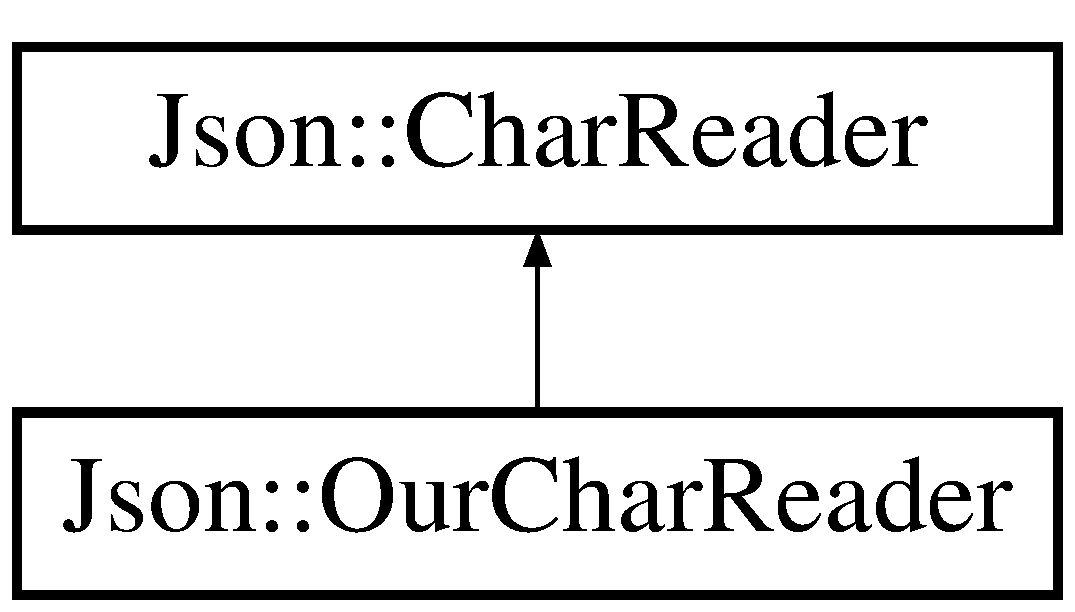
\includegraphics[height=2.000000cm]{classJson_1_1OurCharReader}
\end{center}
\end{figure}
\subsection*{Public Member Functions}
\begin{DoxyCompactItemize}
\item 
\mbox{\Hypertarget{classJson_1_1OurCharReader_a5015506620e7ba7bab417756fa1ca9fe}\label{classJson_1_1OurCharReader_a5015506620e7ba7bab417756fa1ca9fe}} 
{\bfseries Our\+Char\+Reader} (bool collect\+Comments, \hyperlink{classJson_1_1OurFeatures}{Our\+Features} const \&features)
\item 
bool \hyperlink{classJson_1_1OurCharReader_a547f08ec5a9951ca69e8bb2e90296c83}{parse} (char const $\ast$begin\+Doc, char const $\ast$end\+Doc, \hyperlink{classJson_1_1Value}{Value} $\ast$root, J\+S\+O\+N\+C\+P\+P\+\_\+\+S\+T\+R\+I\+NG $\ast$errs) J\+S\+O\+N\+C\+P\+P\+\_\+\+O\+V\+E\+R\+R\+I\+DE
\begin{DoxyCompactList}\small\item\em Read a \hyperlink{classJson_1_1Value}{Value} from a \href{http://www.json.org}{\tt J\+S\+ON} document. The document must be a U\+T\+F-\/8 encoded string containing the document to read. \end{DoxyCompactList}\end{DoxyCompactItemize}


\subsection{Member Function Documentation}
\mbox{\Hypertarget{classJson_1_1OurCharReader_a547f08ec5a9951ca69e8bb2e90296c83}\label{classJson_1_1OurCharReader_a547f08ec5a9951ca69e8bb2e90296c83}} 
\index{Json\+::\+Our\+Char\+Reader@{Json\+::\+Our\+Char\+Reader}!parse@{parse}}
\index{parse@{parse}!Json\+::\+Our\+Char\+Reader@{Json\+::\+Our\+Char\+Reader}}
\subsubsection{\texorpdfstring{parse()}{parse()}}
{\footnotesize\ttfamily bool Json\+::\+Our\+Char\+Reader\+::parse (\begin{DoxyParamCaption}\item[{char const $\ast$}]{begin\+Doc,  }\item[{char const $\ast$}]{end\+Doc,  }\item[{\hyperlink{classJson_1_1Value}{Value} $\ast$}]{root,  }\item[{J\+S\+O\+N\+C\+P\+P\+\_\+\+S\+T\+R\+I\+NG $\ast$}]{errs }\end{DoxyParamCaption})\hspace{0.3cm}{\ttfamily [inline]}, {\ttfamily [virtual]}}



Read a \hyperlink{classJson_1_1Value}{Value} from a \href{http://www.json.org}{\tt J\+S\+ON} document. The document must be a U\+T\+F-\/8 encoded string containing the document to read. 


\begin{DoxyParams}{Parameters}
{\em begin\+Doc} & Pointer on the beginning of the U\+T\+F-\/8 encoded string of the document to read. \\
\hline
{\em end\+Doc} & Pointer on the end of the U\+T\+F-\/8 encoded string of the document to read. Must be $>$= begin\+Doc. \\
\hline
{\em root} & \mbox{[}out\mbox{]} Contains the root value of the document if it was successfully parsed. \\
\hline
{\em errs} & \mbox{[}out\mbox{]} Formatted error messages (if not N\+U\+LL) a user friendly string that lists errors in the parsed document. \\
\hline
\end{DoxyParams}
\begin{DoxyReturn}{Returns}
{\ttfamily true} if the document was successfully parsed, {\ttfamily false} if an error occurred. 
\end{DoxyReturn}


Implements \hyperlink{classJson_1_1CharReader_a7983680d50fd0745f371c43b162e78e1}{Json\+::\+Char\+Reader}.



The documentation for this class was generated from the following file\+:\begin{DoxyCompactItemize}
\item 
jsoncpp.\+cpp\end{DoxyCompactItemize}

\hypertarget{classJson_1_1OurFeatures}{}\section{Json\+:\+:Our\+Features Class Reference}
\label{classJson_1_1OurFeatures}\index{Json\+::\+Our\+Features@{Json\+::\+Our\+Features}}
\subsection*{Static Public Member Functions}
\begin{DoxyCompactItemize}
\item 
\mbox{\Hypertarget{classJson_1_1OurFeatures_a0686e1406b6677f496529f9f3fe98d1e}\label{classJson_1_1OurFeatures_a0686e1406b6677f496529f9f3fe98d1e}} 
static \hyperlink{classJson_1_1OurFeatures}{Our\+Features} {\bfseries all} ()
\end{DoxyCompactItemize}
\subsection*{Public Attributes}
\begin{DoxyCompactItemize}
\item 
\mbox{\Hypertarget{classJson_1_1OurFeatures_ac71bb7ba7363d3b05ed76602b036ce33}\label{classJson_1_1OurFeatures_ac71bb7ba7363d3b05ed76602b036ce33}} 
bool {\bfseries allow\+Comments\+\_\+}
\item 
\mbox{\Hypertarget{classJson_1_1OurFeatures_a2095f66a776c0a4ae6cc931a0c94242e}\label{classJson_1_1OurFeatures_a2095f66a776c0a4ae6cc931a0c94242e}} 
bool {\bfseries strict\+Root\+\_\+}
\item 
\mbox{\Hypertarget{classJson_1_1OurFeatures_a13963bc44bf948eec1968f7ff8e8f5f1}\label{classJson_1_1OurFeatures_a13963bc44bf948eec1968f7ff8e8f5f1}} 
bool {\bfseries allow\+Dropped\+Null\+Placeholders\+\_\+}
\item 
\mbox{\Hypertarget{classJson_1_1OurFeatures_af6973fc7e774ce2d634ba99442aeb91a}\label{classJson_1_1OurFeatures_af6973fc7e774ce2d634ba99442aeb91a}} 
bool {\bfseries allow\+Numeric\+Keys\+\_\+}
\item 
\mbox{\Hypertarget{classJson_1_1OurFeatures_abbd6c196d7a22e2a360a59887eda4610}\label{classJson_1_1OurFeatures_abbd6c196d7a22e2a360a59887eda4610}} 
bool {\bfseries allow\+Single\+Quotes\+\_\+}
\item 
\mbox{\Hypertarget{classJson_1_1OurFeatures_ae8ad25b90706c78f1a8fe929191ac61b}\label{classJson_1_1OurFeatures_ae8ad25b90706c78f1a8fe929191ac61b}} 
bool {\bfseries fail\+If\+Extra\+\_\+}
\item 
\mbox{\Hypertarget{classJson_1_1OurFeatures_a39b8e0b86b1c24a45e800c023bb715aa}\label{classJson_1_1OurFeatures_a39b8e0b86b1c24a45e800c023bb715aa}} 
bool {\bfseries reject\+Dup\+Keys\+\_\+}
\item 
\mbox{\Hypertarget{classJson_1_1OurFeatures_af760f91cc2a7af37e44f78fb466061bb}\label{classJson_1_1OurFeatures_af760f91cc2a7af37e44f78fb466061bb}} 
bool {\bfseries allow\+Special\+Floats\+\_\+}
\item 
\mbox{\Hypertarget{classJson_1_1OurFeatures_a9a786713902d14be6d57a08cc03ccfff}\label{classJson_1_1OurFeatures_a9a786713902d14be6d57a08cc03ccfff}} 
int {\bfseries stack\+Limit\+\_\+}
\end{DoxyCompactItemize}


The documentation for this class was generated from the following file\+:\begin{DoxyCompactItemize}
\item 
jsoncpp.\+cpp\end{DoxyCompactItemize}

\hypertarget{classJson_1_1OurReader}{}\section{Json\+:\+:Our\+Reader Class Reference}
\label{classJson_1_1OurReader}\index{Json\+::\+Our\+Reader@{Json\+::\+Our\+Reader}}
\subsection*{Classes}
\begin{DoxyCompactItemize}
\item 
class \hyperlink{classJson_1_1OurReader_1_1ErrorInfo}{Error\+Info}
\item 
struct \hyperlink{structJson_1_1OurReader_1_1StructuredError}{Structured\+Error}
\item 
class \hyperlink{classJson_1_1OurReader_1_1Token}{Token}
\end{DoxyCompactItemize}
\subsection*{Public Types}
\begin{DoxyCompactItemize}
\item 
typedef char \hyperlink{classJson_1_1OurReader_a0cd0bab4caa66594ab843ccd5f9dc239_a0cd0bab4caa66594ab843ccd5f9dc239}{Char}
\item 
typedef const \hyperlink{classJson_1_1OurReader_a0cd0bab4caa66594ab843ccd5f9dc239_a0cd0bab4caa66594ab843ccd5f9dc239}{Char} $\ast$ \hyperlink{classJson_1_1OurReader_a1bdc7bbc52ba87cae6b19746f2ee0189_a1bdc7bbc52ba87cae6b19746f2ee0189}{Location}
\end{DoxyCompactItemize}
\subsection*{Public Member Functions}
\begin{DoxyCompactItemize}
\item 
\hyperlink{classJson_1_1OurReader_a48a850914b9c8d7781be172930c478e5_a48a850914b9c8d7781be172930c478e5}{Our\+Reader} (\hyperlink{classJson_1_1OurFeatures}{Our\+Features} const \&features)
\item 
bool \hyperlink{classJson_1_1OurReader_aba4f8749aab7f02ec17f107e392caf80_aba4f8749aab7f02ec17f107e392caf80}{parse} (const char $\ast$begin\+Doc, const char $\ast$end\+Doc, \hyperlink{classJson_1_1Value}{Value} \&root, bool collect\+Comments=true)
\item 
\hyperlink{json_8h_a1e723f95759de062585bc4a8fd3fa4be_a1e723f95759de062585bc4a8fd3fa4be}{J\+S\+O\+N\+C\+P\+P\+\_\+\+S\+T\+R\+I\+NG} \hyperlink{classJson_1_1OurReader_a7971de51d73bb4aee5b0c4742c4aaaac_a7971de51d73bb4aee5b0c4742c4aaaac}{get\+Formatted\+Error\+Messages} () const
\item 
std\+::vector$<$ \hyperlink{structJson_1_1OurReader_1_1StructuredError}{Structured\+Error} $>$ \hyperlink{classJson_1_1OurReader_a0eb2420a6bef89a3f3256191e6e3de6d_a0eb2420a6bef89a3f3256191e6e3de6d}{get\+Structured\+Errors} () const
\item 
bool \hyperlink{classJson_1_1OurReader_a700e9d8e0977fa7e0375d26690d7025f_a700e9d8e0977fa7e0375d26690d7025f}{push\+Error} (const \hyperlink{classJson_1_1Value}{Value} \&value, const \hyperlink{json_8h_a1e723f95759de062585bc4a8fd3fa4be_a1e723f95759de062585bc4a8fd3fa4be}{J\+S\+O\+N\+C\+P\+P\+\_\+\+S\+T\+R\+I\+NG} \&message)
\item 
bool \hyperlink{classJson_1_1OurReader_addccecfca74b79adaad6115ddd614477_addccecfca74b79adaad6115ddd614477}{push\+Error} (const \hyperlink{classJson_1_1Value}{Value} \&value, const \hyperlink{json_8h_a1e723f95759de062585bc4a8fd3fa4be_a1e723f95759de062585bc4a8fd3fa4be}{J\+S\+O\+N\+C\+P\+P\+\_\+\+S\+T\+R\+I\+NG} \&message, const \hyperlink{classJson_1_1Value}{Value} \&extra)
\item 
bool \hyperlink{classJson_1_1OurReader_a63c7d874fa379397e0a5fa65f0843845_a63c7d874fa379397e0a5fa65f0843845}{good} () const
\end{DoxyCompactItemize}
\subsection*{Private Types}
\begin{DoxyCompactItemize}
\item 
enum \hyperlink{classJson_1_1OurReader_a15116f7276ddf1e7a2cc3cbefa884dcc_a15116f7276ddf1e7a2cc3cbefa884dcc}{Token\+Type} \{ \newline
\hyperlink{classJson_1_1OurReader_a15116f7276ddf1e7a2cc3cbefa884dcc_a15116f7276ddf1e7a2cc3cbefa884dcca735d1f76eafc2c0c581ed79c077aaa7e}{token\+End\+Of\+Stream} = 0, 
\hyperlink{classJson_1_1OurReader_a15116f7276ddf1e7a2cc3cbefa884dcc_a15116f7276ddf1e7a2cc3cbefa884dcca7495ef5c356d4faa39b702e528cc7e26}{token\+Object\+Begin}, 
\hyperlink{classJson_1_1OurReader_a15116f7276ddf1e7a2cc3cbefa884dcc_a15116f7276ddf1e7a2cc3cbefa884dcca8d7e94be97d76ea1c314130b5aabb014}{token\+Object\+End}, 
\hyperlink{classJson_1_1OurReader_a15116f7276ddf1e7a2cc3cbefa884dcc_a15116f7276ddf1e7a2cc3cbefa884dcca45d229fce2f5f4b52dc0d6c39c853436}{token\+Array\+Begin}, 
\newline
\hyperlink{classJson_1_1OurReader_a15116f7276ddf1e7a2cc3cbefa884dcc_a15116f7276ddf1e7a2cc3cbefa884dcca59a4f42b50d9731dce6be41818c3d91b}{token\+Array\+End}, 
\hyperlink{classJson_1_1OurReader_a15116f7276ddf1e7a2cc3cbefa884dcc_a15116f7276ddf1e7a2cc3cbefa884dccadb37e59e1e52cd5e7417bc418b611ce1}{token\+String}, 
\hyperlink{classJson_1_1OurReader_a15116f7276ddf1e7a2cc3cbefa884dcc_a15116f7276ddf1e7a2cc3cbefa884dcca766aefde855b1246d89b8552240c70d1}{token\+Number}, 
\hyperlink{classJson_1_1OurReader_a15116f7276ddf1e7a2cc3cbefa884dcc_a15116f7276ddf1e7a2cc3cbefa884dccac7d2a552afcea291d47cf49dfefaf619}{token\+True}, 
\newline
\hyperlink{classJson_1_1OurReader_a15116f7276ddf1e7a2cc3cbefa884dcc_a15116f7276ddf1e7a2cc3cbefa884dccaab91e3ef98c1cb1326c3674e518c5126}{token\+False}, 
\hyperlink{classJson_1_1OurReader_a15116f7276ddf1e7a2cc3cbefa884dcc_a15116f7276ddf1e7a2cc3cbefa884dcca4c80b7bb245e3863e38dc8e8586b3c51}{token\+Null}, 
\hyperlink{classJson_1_1OurReader_a15116f7276ddf1e7a2cc3cbefa884dcc_a15116f7276ddf1e7a2cc3cbefa884dcca167898478691f1ac7a240981ccaa1713}{token\+NaN}, 
\hyperlink{classJson_1_1OurReader_a15116f7276ddf1e7a2cc3cbefa884dcc_a15116f7276ddf1e7a2cc3cbefa884dcca800c7c7e896d569ebf6c2771eecc7060}{token\+Pos\+Inf}, 
\newline
\hyperlink{classJson_1_1OurReader_a15116f7276ddf1e7a2cc3cbefa884dcc_a15116f7276ddf1e7a2cc3cbefa884dcca3cf3c4c72d6b5969f17f043a34b2ad4c}{token\+Neg\+Inf}, 
\hyperlink{classJson_1_1OurReader_a15116f7276ddf1e7a2cc3cbefa884dcc_a15116f7276ddf1e7a2cc3cbefa884dcca8ca62ab9091b149d52ec55828f8040f4}{token\+Array\+Separator}, 
\hyperlink{classJson_1_1OurReader_a15116f7276ddf1e7a2cc3cbefa884dcc_a15116f7276ddf1e7a2cc3cbefa884dcca7c95881fb1162316bce42c629bf06214}{token\+Member\+Separator}, 
\hyperlink{classJson_1_1OurReader_a15116f7276ddf1e7a2cc3cbefa884dcc_a15116f7276ddf1e7a2cc3cbefa884dcca777fb6589fdbe225bc10a1e49a090da9}{token\+Comment}, 
\newline
\hyperlink{classJson_1_1OurReader_a15116f7276ddf1e7a2cc3cbefa884dcc_a15116f7276ddf1e7a2cc3cbefa884dccad39f929b971de8dc55fe84a2d2e3465e}{token\+Error}
 \}
\item 
typedef std\+::deque$<$ \hyperlink{classJson_1_1OurReader_1_1ErrorInfo}{Error\+Info} $>$ \hyperlink{classJson_1_1OurReader_a8cc69593ef7303e58e99bb5dbb767562_a8cc69593ef7303e58e99bb5dbb767562}{Errors}
\item 
typedef std\+::stack$<$ \hyperlink{classJson_1_1Value}{Value} $\ast$ $>$ \hyperlink{classJson_1_1OurReader_a8480a5ef159cee3a090f96358414d8d3_a8480a5ef159cee3a090f96358414d8d3}{Nodes}
\end{DoxyCompactItemize}
\subsection*{Private Member Functions}
\begin{DoxyCompactItemize}
\item 
\hyperlink{classJson_1_1OurReader_aee013005522c0d34d2e14962851487ac_aee013005522c0d34d2e14962851487ac}{Our\+Reader} (\hyperlink{classJson_1_1OurReader}{Our\+Reader} const \&)
\item 
void \hyperlink{classJson_1_1OurReader_ad418de7c47bd3d0510888e22110b796e_ad418de7c47bd3d0510888e22110b796e}{operator=} (\hyperlink{classJson_1_1OurReader}{Our\+Reader} const \&)
\item 
bool \hyperlink{classJson_1_1OurReader_a0d1e66da47fe2e85f5033c59326dfdc3_a0d1e66da47fe2e85f5033c59326dfdc3}{read\+Token} (\hyperlink{classJson_1_1OurReader_1_1Token}{Token} \&token)
\item 
void \hyperlink{classJson_1_1OurReader_a6fbc6d58a4505e5ccadf330b57b17ca5_a6fbc6d58a4505e5ccadf330b57b17ca5}{skip\+Spaces} ()
\item 
bool \hyperlink{classJson_1_1OurReader_a4a03f1b266def9b47c4fef35386557fb_a4a03f1b266def9b47c4fef35386557fb}{match} (\hyperlink{classJson_1_1OurReader_a1bdc7bbc52ba87cae6b19746f2ee0189_a1bdc7bbc52ba87cae6b19746f2ee0189}{Location} pattern, int pattern\+Length)
\item 
bool \hyperlink{classJson_1_1OurReader_a90f6bb9e55b2bc3d6c1880809495c222_a90f6bb9e55b2bc3d6c1880809495c222}{read\+Comment} ()
\item 
bool \hyperlink{classJson_1_1OurReader_aba784b125baa1b62387e767b791f2f89_aba784b125baa1b62387e767b791f2f89}{read\+C\+Style\+Comment} ()
\item 
bool \hyperlink{classJson_1_1OurReader_ae3de80671f0f997053e1c1c8a47a45c5_ae3de80671f0f997053e1c1c8a47a45c5}{read\+Cpp\+Style\+Comment} ()
\item 
bool \hyperlink{classJson_1_1OurReader_a5d39b12671499ec5975f3bbc84b7d438_a5d39b12671499ec5975f3bbc84b7d438}{read\+String} ()
\item 
bool \hyperlink{classJson_1_1OurReader_ac78592defdc333faf56c6d0908758da3_ac78592defdc333faf56c6d0908758da3}{read\+String\+Single\+Quote} ()
\item 
bool \hyperlink{classJson_1_1OurReader_aefcb9a78cc45870ccac2db2a66c8ec50_aefcb9a78cc45870ccac2db2a66c8ec50}{read\+Number} (bool check\+Inf)
\item 
bool \hyperlink{classJson_1_1OurReader_a1765d9670d191c89a57a22ea5591d35f_a1765d9670d191c89a57a22ea5591d35f}{read\+Value} ()
\item 
bool \hyperlink{classJson_1_1OurReader_aea198f8101dba55099f4d8121a993530_aea198f8101dba55099f4d8121a993530}{read\+Object} (\hyperlink{classJson_1_1OurReader_1_1Token}{Token} \&token)
\item 
bool \hyperlink{classJson_1_1OurReader_a0b9f58faf4212c6ecb5d8e2a1ac10257_a0b9f58faf4212c6ecb5d8e2a1ac10257}{read\+Array} (\hyperlink{classJson_1_1OurReader_1_1Token}{Token} \&token)
\item 
bool \hyperlink{classJson_1_1OurReader_a272d271290933a89abfd5096dd69c9e9_a272d271290933a89abfd5096dd69c9e9}{decode\+Number} (\hyperlink{classJson_1_1OurReader_1_1Token}{Token} \&token)
\item 
bool \hyperlink{classJson_1_1OurReader_a712270d53a2f023c2f406ac813548340_a712270d53a2f023c2f406ac813548340}{decode\+Number} (\hyperlink{classJson_1_1OurReader_1_1Token}{Token} \&token, \hyperlink{classJson_1_1Value}{Value} \&decoded)
\item 
bool \hyperlink{classJson_1_1OurReader_a34e31d8b8399b7ad493359702b6de6c9_a34e31d8b8399b7ad493359702b6de6c9}{decode\+String} (\hyperlink{classJson_1_1OurReader_1_1Token}{Token} \&token)
\item 
bool \hyperlink{classJson_1_1OurReader_a5046dfa5d43b1770a091aac0a63a9f4b_a5046dfa5d43b1770a091aac0a63a9f4b}{decode\+String} (\hyperlink{classJson_1_1OurReader_1_1Token}{Token} \&token, \hyperlink{json_8h_a1e723f95759de062585bc4a8fd3fa4be_a1e723f95759de062585bc4a8fd3fa4be}{J\+S\+O\+N\+C\+P\+P\+\_\+\+S\+T\+R\+I\+NG} \&decoded)
\item 
bool \hyperlink{classJson_1_1OurReader_a1d1c3b44f6720a0e7c39b5ae8de3981c_a1d1c3b44f6720a0e7c39b5ae8de3981c}{decode\+Double} (\hyperlink{classJson_1_1OurReader_1_1Token}{Token} \&token)
\item 
bool \hyperlink{classJson_1_1OurReader_aa5c15a8cd32754f07430dedba3d1308e_aa5c15a8cd32754f07430dedba3d1308e}{decode\+Double} (\hyperlink{classJson_1_1OurReader_1_1Token}{Token} \&token, \hyperlink{classJson_1_1Value}{Value} \&decoded)
\item 
bool \hyperlink{classJson_1_1OurReader_ac1bf03c161ece082e48da450c50f528d_ac1bf03c161ece082e48da450c50f528d}{decode\+Unicode\+Code\+Point} (\hyperlink{classJson_1_1OurReader_1_1Token}{Token} \&token, \hyperlink{classJson_1_1OurReader_a1bdc7bbc52ba87cae6b19746f2ee0189_a1bdc7bbc52ba87cae6b19746f2ee0189}{Location} \&current, \hyperlink{classJson_1_1OurReader_a1bdc7bbc52ba87cae6b19746f2ee0189_a1bdc7bbc52ba87cae6b19746f2ee0189}{Location} end, unsigned int \&unicode)
\item 
bool \hyperlink{classJson_1_1OurReader_adb39be814cc6076b91a0919bdd5b24b0_adb39be814cc6076b91a0919bdd5b24b0}{decode\+Unicode\+Escape\+Sequence} (\hyperlink{classJson_1_1OurReader_1_1Token}{Token} \&token, \hyperlink{classJson_1_1OurReader_a1bdc7bbc52ba87cae6b19746f2ee0189_a1bdc7bbc52ba87cae6b19746f2ee0189}{Location} \&current, \hyperlink{classJson_1_1OurReader_a1bdc7bbc52ba87cae6b19746f2ee0189_a1bdc7bbc52ba87cae6b19746f2ee0189}{Location} end, unsigned int \&unicode)
\item 
bool \hyperlink{classJson_1_1OurReader_aa6a920311e6408ff3a45324d49da18a6_aa6a920311e6408ff3a45324d49da18a6}{add\+Error} (const \hyperlink{json_8h_a1e723f95759de062585bc4a8fd3fa4be_a1e723f95759de062585bc4a8fd3fa4be}{J\+S\+O\+N\+C\+P\+P\+\_\+\+S\+T\+R\+I\+NG} \&message, \hyperlink{classJson_1_1OurReader_1_1Token}{Token} \&token, \hyperlink{classJson_1_1OurReader_a1bdc7bbc52ba87cae6b19746f2ee0189_a1bdc7bbc52ba87cae6b19746f2ee0189}{Location} extra=0)
\item 
bool \hyperlink{classJson_1_1OurReader_a035651f0700a76a815e5f904c63ebb1c_a035651f0700a76a815e5f904c63ebb1c}{recover\+From\+Error} (\hyperlink{classJson_1_1OurReader_a15116f7276ddf1e7a2cc3cbefa884dcc_a15116f7276ddf1e7a2cc3cbefa884dcc}{Token\+Type} skip\+Until\+Token)
\item 
bool \hyperlink{classJson_1_1OurReader_a074cf3d91e9404fe89e03cfc6a43e6fb_a074cf3d91e9404fe89e03cfc6a43e6fb}{add\+Error\+And\+Recover} (const \hyperlink{json_8h_a1e723f95759de062585bc4a8fd3fa4be_a1e723f95759de062585bc4a8fd3fa4be}{J\+S\+O\+N\+C\+P\+P\+\_\+\+S\+T\+R\+I\+NG} \&message, \hyperlink{classJson_1_1OurReader_1_1Token}{Token} \&token, \hyperlink{classJson_1_1OurReader_a15116f7276ddf1e7a2cc3cbefa884dcc_a15116f7276ddf1e7a2cc3cbefa884dcc}{Token\+Type} skip\+Until\+Token)
\item 
void \hyperlink{classJson_1_1OurReader_ad48bdaf5b686706f003e792fdbcbf102_ad48bdaf5b686706f003e792fdbcbf102}{skip\+Until\+Space} ()
\item 
\hyperlink{classJson_1_1Value}{Value} \& \hyperlink{classJson_1_1OurReader_a2acd5b1d53e7d7e17c21ff8e96edc09d_a2acd5b1d53e7d7e17c21ff8e96edc09d}{current\+Value} ()
\item 
\hyperlink{classJson_1_1OurReader_a0cd0bab4caa66594ab843ccd5f9dc239_a0cd0bab4caa66594ab843ccd5f9dc239}{Char} \hyperlink{classJson_1_1OurReader_a298285d035fdbc554caae09d9f0a5859_a298285d035fdbc554caae09d9f0a5859}{get\+Next\+Char} ()
\item 
void \hyperlink{classJson_1_1OurReader_af482c8e718615646e13a996292e18d74_af482c8e718615646e13a996292e18d74}{get\+Location\+Line\+And\+Column} (\hyperlink{classJson_1_1OurReader_a1bdc7bbc52ba87cae6b19746f2ee0189_a1bdc7bbc52ba87cae6b19746f2ee0189}{Location} location, int \&line, int \&column) const
\item 
\hyperlink{json_8h_a1e723f95759de062585bc4a8fd3fa4be_a1e723f95759de062585bc4a8fd3fa4be}{J\+S\+O\+N\+C\+P\+P\+\_\+\+S\+T\+R\+I\+NG} \hyperlink{classJson_1_1OurReader_ac129e94cdc260822b2fd24e2ca35e636_ac129e94cdc260822b2fd24e2ca35e636}{get\+Location\+Line\+And\+Column} (\hyperlink{classJson_1_1OurReader_a1bdc7bbc52ba87cae6b19746f2ee0189_a1bdc7bbc52ba87cae6b19746f2ee0189}{Location} location) const
\item 
void \hyperlink{classJson_1_1OurReader_ad7318c37469a9106069a236fb4b10e1f_ad7318c37469a9106069a236fb4b10e1f}{add\+Comment} (\hyperlink{classJson_1_1OurReader_a1bdc7bbc52ba87cae6b19746f2ee0189_a1bdc7bbc52ba87cae6b19746f2ee0189}{Location} begin, \hyperlink{classJson_1_1OurReader_a1bdc7bbc52ba87cae6b19746f2ee0189_a1bdc7bbc52ba87cae6b19746f2ee0189}{Location} end, \hyperlink{namespaceJson_a4fc417c23905b2ae9e2c47d197a45351_a4fc417c23905b2ae9e2c47d197a45351}{Comment\+Placement} placement)
\item 
void \hyperlink{classJson_1_1OurReader_a856dea44d92578c276856d7a65a4ebdc_a856dea44d92578c276856d7a65a4ebdc}{skip\+Comment\+Tokens} (\hyperlink{classJson_1_1OurReader_1_1Token}{Token} \&token)
\end{DoxyCompactItemize}
\subsection*{Static Private Member Functions}
\begin{DoxyCompactItemize}
\item 
static \hyperlink{json_8h_a1e723f95759de062585bc4a8fd3fa4be_a1e723f95759de062585bc4a8fd3fa4be}{J\+S\+O\+N\+C\+P\+P\+\_\+\+S\+T\+R\+I\+NG} \hyperlink{classJson_1_1OurReader_a73ec369ee36598e008b80e36263691be_a73ec369ee36598e008b80e36263691be}{normalize\+E\+OL} (\hyperlink{classJson_1_1OurReader_a1bdc7bbc52ba87cae6b19746f2ee0189_a1bdc7bbc52ba87cae6b19746f2ee0189}{Location} begin, \hyperlink{classJson_1_1OurReader_a1bdc7bbc52ba87cae6b19746f2ee0189_a1bdc7bbc52ba87cae6b19746f2ee0189}{Location} end)
\item 
static bool \hyperlink{classJson_1_1OurReader_ab9e83f5a3d9dab2dabce367a4faa2b1b_ab9e83f5a3d9dab2dabce367a4faa2b1b}{contains\+New\+Line} (\hyperlink{classJson_1_1OurReader_a1bdc7bbc52ba87cae6b19746f2ee0189_a1bdc7bbc52ba87cae6b19746f2ee0189}{Location} begin, \hyperlink{classJson_1_1OurReader_a1bdc7bbc52ba87cae6b19746f2ee0189_a1bdc7bbc52ba87cae6b19746f2ee0189}{Location} end)
\end{DoxyCompactItemize}
\subsection*{Private Attributes}
\begin{DoxyCompactItemize}
\item 
\hyperlink{classJson_1_1OurReader_a8480a5ef159cee3a090f96358414d8d3_a8480a5ef159cee3a090f96358414d8d3}{Nodes} \hyperlink{classJson_1_1OurReader_a19cc4e8c5d17ee6822f752e9a36f4ce3_a19cc4e8c5d17ee6822f752e9a36f4ce3}{nodes\+\_\+}
\item 
\hyperlink{classJson_1_1OurReader_a8cc69593ef7303e58e99bb5dbb767562_a8cc69593ef7303e58e99bb5dbb767562}{Errors} \hyperlink{classJson_1_1OurReader_afb76b68ba1ab68fe09cf2838e3d4898d_afb76b68ba1ab68fe09cf2838e3d4898d}{errors\+\_\+}
\item 
\hyperlink{json_8h_a1e723f95759de062585bc4a8fd3fa4be_a1e723f95759de062585bc4a8fd3fa4be}{J\+S\+O\+N\+C\+P\+P\+\_\+\+S\+T\+R\+I\+NG} \hyperlink{classJson_1_1OurReader_a726230af83d22d25e0c76cec3408ecf1_a726230af83d22d25e0c76cec3408ecf1}{document\+\_\+}
\item 
\hyperlink{classJson_1_1OurReader_a1bdc7bbc52ba87cae6b19746f2ee0189_a1bdc7bbc52ba87cae6b19746f2ee0189}{Location} \hyperlink{classJson_1_1OurReader_a9bda9d72335d52cd06e65f9eca3f70f5_a9bda9d72335d52cd06e65f9eca3f70f5}{begin\+\_\+}
\item 
\hyperlink{classJson_1_1OurReader_a1bdc7bbc52ba87cae6b19746f2ee0189_a1bdc7bbc52ba87cae6b19746f2ee0189}{Location} \hyperlink{classJson_1_1OurReader_ab1f69b0260c27a0d2d65dc56e42c8f9d_ab1f69b0260c27a0d2d65dc56e42c8f9d}{end\+\_\+}
\item 
\hyperlink{classJson_1_1OurReader_a1bdc7bbc52ba87cae6b19746f2ee0189_a1bdc7bbc52ba87cae6b19746f2ee0189}{Location} \hyperlink{classJson_1_1OurReader_a5211fbbba94be80a22dd2317c621efcc_a5211fbbba94be80a22dd2317c621efcc}{current\+\_\+}
\item 
\hyperlink{classJson_1_1OurReader_a1bdc7bbc52ba87cae6b19746f2ee0189_a1bdc7bbc52ba87cae6b19746f2ee0189}{Location} \hyperlink{classJson_1_1OurReader_a101eadc45e01c60628b53f0db3d13482_a101eadc45e01c60628b53f0db3d13482}{last\+Value\+End\+\_\+}
\item 
\hyperlink{classJson_1_1Value}{Value} $\ast$ \hyperlink{classJson_1_1OurReader_a9f994b6a2227c5d96e6ed6cbc74ed251_a9f994b6a2227c5d96e6ed6cbc74ed251}{last\+Value\+\_\+}
\item 
\hyperlink{json_8h_a1e723f95759de062585bc4a8fd3fa4be_a1e723f95759de062585bc4a8fd3fa4be}{J\+S\+O\+N\+C\+P\+P\+\_\+\+S\+T\+R\+I\+NG} \hyperlink{classJson_1_1OurReader_a9c53e77e290eb9081298210a955fda6a_a9c53e77e290eb9081298210a955fda6a}{comments\+Before\+\_\+}
\item 
\hyperlink{classJson_1_1OurFeatures}{Our\+Features} const \hyperlink{classJson_1_1OurReader_a2714302d5cc54ca2ce4118ea51c0397a_a2714302d5cc54ca2ce4118ea51c0397a}{features\+\_\+}
\item 
bool \hyperlink{classJson_1_1OurReader_a259f6ac988da2894bcafc670e42f73ad_a259f6ac988da2894bcafc670e42f73ad}{collect\+Comments\+\_\+}
\end{DoxyCompactItemize}


\subsection{Member Typedef Documentation}
\mbox{\Hypertarget{classJson_1_1OurReader_a0cd0bab4caa66594ab843ccd5f9dc239_a0cd0bab4caa66594ab843ccd5f9dc239}\label{classJson_1_1OurReader_a0cd0bab4caa66594ab843ccd5f9dc239_a0cd0bab4caa66594ab843ccd5f9dc239}} 
\index{Json\+::\+Our\+Reader@{Json\+::\+Our\+Reader}!Char@{Char}}
\index{Char@{Char}!Json\+::\+Our\+Reader@{Json\+::\+Our\+Reader}}
\subsubsection{\texorpdfstring{Char}{Char}}
{\footnotesize\ttfamily typedef char \hyperlink{classJson_1_1OurReader_a0cd0bab4caa66594ab843ccd5f9dc239_a0cd0bab4caa66594ab843ccd5f9dc239}{Json\+::\+Our\+Reader\+::\+Char}}

\mbox{\Hypertarget{classJson_1_1OurReader_a8cc69593ef7303e58e99bb5dbb767562_a8cc69593ef7303e58e99bb5dbb767562}\label{classJson_1_1OurReader_a8cc69593ef7303e58e99bb5dbb767562_a8cc69593ef7303e58e99bb5dbb767562}} 
\index{Json\+::\+Our\+Reader@{Json\+::\+Our\+Reader}!Errors@{Errors}}
\index{Errors@{Errors}!Json\+::\+Our\+Reader@{Json\+::\+Our\+Reader}}
\subsubsection{\texorpdfstring{Errors}{Errors}}
{\footnotesize\ttfamily typedef std\+::deque$<$\hyperlink{classJson_1_1OurReader_1_1ErrorInfo}{Error\+Info}$>$ \hyperlink{classJson_1_1OurReader_a8cc69593ef7303e58e99bb5dbb767562_a8cc69593ef7303e58e99bb5dbb767562}{Json\+::\+Our\+Reader\+::\+Errors}\hspace{0.3cm}{\ttfamily [private]}}

\mbox{\Hypertarget{classJson_1_1OurReader_a1bdc7bbc52ba87cae6b19746f2ee0189_a1bdc7bbc52ba87cae6b19746f2ee0189}\label{classJson_1_1OurReader_a1bdc7bbc52ba87cae6b19746f2ee0189_a1bdc7bbc52ba87cae6b19746f2ee0189}} 
\index{Json\+::\+Our\+Reader@{Json\+::\+Our\+Reader}!Location@{Location}}
\index{Location@{Location}!Json\+::\+Our\+Reader@{Json\+::\+Our\+Reader}}
\subsubsection{\texorpdfstring{Location}{Location}}
{\footnotesize\ttfamily typedef const \hyperlink{classJson_1_1OurReader_a0cd0bab4caa66594ab843ccd5f9dc239_a0cd0bab4caa66594ab843ccd5f9dc239}{Char}$\ast$ \hyperlink{classJson_1_1OurReader_a1bdc7bbc52ba87cae6b19746f2ee0189_a1bdc7bbc52ba87cae6b19746f2ee0189}{Json\+::\+Our\+Reader\+::\+Location}}

\mbox{\Hypertarget{classJson_1_1OurReader_a8480a5ef159cee3a090f96358414d8d3_a8480a5ef159cee3a090f96358414d8d3}\label{classJson_1_1OurReader_a8480a5ef159cee3a090f96358414d8d3_a8480a5ef159cee3a090f96358414d8d3}} 
\index{Json\+::\+Our\+Reader@{Json\+::\+Our\+Reader}!Nodes@{Nodes}}
\index{Nodes@{Nodes}!Json\+::\+Our\+Reader@{Json\+::\+Our\+Reader}}
\subsubsection{\texorpdfstring{Nodes}{Nodes}}
{\footnotesize\ttfamily typedef std\+::stack$<$\hyperlink{classJson_1_1Value}{Value}$\ast$$>$ \hyperlink{classJson_1_1OurReader_a8480a5ef159cee3a090f96358414d8d3_a8480a5ef159cee3a090f96358414d8d3}{Json\+::\+Our\+Reader\+::\+Nodes}\hspace{0.3cm}{\ttfamily [private]}}



\subsection{Member Enumeration Documentation}
\mbox{\Hypertarget{classJson_1_1OurReader_a15116f7276ddf1e7a2cc3cbefa884dcc_a15116f7276ddf1e7a2cc3cbefa884dcc}\label{classJson_1_1OurReader_a15116f7276ddf1e7a2cc3cbefa884dcc_a15116f7276ddf1e7a2cc3cbefa884dcc}} 
\index{Json\+::\+Our\+Reader@{Json\+::\+Our\+Reader}!Token\+Type@{Token\+Type}}
\index{Token\+Type@{Token\+Type}!Json\+::\+Our\+Reader@{Json\+::\+Our\+Reader}}
\subsubsection{\texorpdfstring{Token\+Type}{TokenType}}
{\footnotesize\ttfamily enum \hyperlink{classJson_1_1OurReader_a15116f7276ddf1e7a2cc3cbefa884dcc_a15116f7276ddf1e7a2cc3cbefa884dcc}{Json\+::\+Our\+Reader\+::\+Token\+Type}\hspace{0.3cm}{\ttfamily [private]}}

\begin{DoxyEnumFields}{Enumerator}
\raisebox{\heightof{T}}[0pt][0pt]{\index{token\+End\+Of\+Stream@{token\+End\+Of\+Stream}!Json\+::\+Our\+Reader@{Json\+::\+Our\+Reader}}\index{Json\+::\+Our\+Reader@{Json\+::\+Our\+Reader}!token\+End\+Of\+Stream@{token\+End\+Of\+Stream}}}\mbox{\Hypertarget{classJson_1_1OurReader_a15116f7276ddf1e7a2cc3cbefa884dcc_a15116f7276ddf1e7a2cc3cbefa884dcca735d1f76eafc2c0c581ed79c077aaa7e}\label{classJson_1_1OurReader_a15116f7276ddf1e7a2cc3cbefa884dcc_a15116f7276ddf1e7a2cc3cbefa884dcca735d1f76eafc2c0c581ed79c077aaa7e}} 
token\+End\+Of\+Stream&\\
\hline

\raisebox{\heightof{T}}[0pt][0pt]{\index{token\+Object\+Begin@{token\+Object\+Begin}!Json\+::\+Our\+Reader@{Json\+::\+Our\+Reader}}\index{Json\+::\+Our\+Reader@{Json\+::\+Our\+Reader}!token\+Object\+Begin@{token\+Object\+Begin}}}\mbox{\Hypertarget{classJson_1_1OurReader_a15116f7276ddf1e7a2cc3cbefa884dcc_a15116f7276ddf1e7a2cc3cbefa884dcca7495ef5c356d4faa39b702e528cc7e26}\label{classJson_1_1OurReader_a15116f7276ddf1e7a2cc3cbefa884dcc_a15116f7276ddf1e7a2cc3cbefa884dcca7495ef5c356d4faa39b702e528cc7e26}} 
token\+Object\+Begin&\\
\hline

\raisebox{\heightof{T}}[0pt][0pt]{\index{token\+Object\+End@{token\+Object\+End}!Json\+::\+Our\+Reader@{Json\+::\+Our\+Reader}}\index{Json\+::\+Our\+Reader@{Json\+::\+Our\+Reader}!token\+Object\+End@{token\+Object\+End}}}\mbox{\Hypertarget{classJson_1_1OurReader_a15116f7276ddf1e7a2cc3cbefa884dcc_a15116f7276ddf1e7a2cc3cbefa884dcca8d7e94be97d76ea1c314130b5aabb014}\label{classJson_1_1OurReader_a15116f7276ddf1e7a2cc3cbefa884dcc_a15116f7276ddf1e7a2cc3cbefa884dcca8d7e94be97d76ea1c314130b5aabb014}} 
token\+Object\+End&\\
\hline

\raisebox{\heightof{T}}[0pt][0pt]{\index{token\+Array\+Begin@{token\+Array\+Begin}!Json\+::\+Our\+Reader@{Json\+::\+Our\+Reader}}\index{Json\+::\+Our\+Reader@{Json\+::\+Our\+Reader}!token\+Array\+Begin@{token\+Array\+Begin}}}\mbox{\Hypertarget{classJson_1_1OurReader_a15116f7276ddf1e7a2cc3cbefa884dcc_a15116f7276ddf1e7a2cc3cbefa884dcca45d229fce2f5f4b52dc0d6c39c853436}\label{classJson_1_1OurReader_a15116f7276ddf1e7a2cc3cbefa884dcc_a15116f7276ddf1e7a2cc3cbefa884dcca45d229fce2f5f4b52dc0d6c39c853436}} 
token\+Array\+Begin&\\
\hline

\raisebox{\heightof{T}}[0pt][0pt]{\index{token\+Array\+End@{token\+Array\+End}!Json\+::\+Our\+Reader@{Json\+::\+Our\+Reader}}\index{Json\+::\+Our\+Reader@{Json\+::\+Our\+Reader}!token\+Array\+End@{token\+Array\+End}}}\mbox{\Hypertarget{classJson_1_1OurReader_a15116f7276ddf1e7a2cc3cbefa884dcc_a15116f7276ddf1e7a2cc3cbefa884dcca59a4f42b50d9731dce6be41818c3d91b}\label{classJson_1_1OurReader_a15116f7276ddf1e7a2cc3cbefa884dcc_a15116f7276ddf1e7a2cc3cbefa884dcca59a4f42b50d9731dce6be41818c3d91b}} 
token\+Array\+End&\\
\hline

\raisebox{\heightof{T}}[0pt][0pt]{\index{token\+String@{token\+String}!Json\+::\+Our\+Reader@{Json\+::\+Our\+Reader}}\index{Json\+::\+Our\+Reader@{Json\+::\+Our\+Reader}!token\+String@{token\+String}}}\mbox{\Hypertarget{classJson_1_1OurReader_a15116f7276ddf1e7a2cc3cbefa884dcc_a15116f7276ddf1e7a2cc3cbefa884dccadb37e59e1e52cd5e7417bc418b611ce1}\label{classJson_1_1OurReader_a15116f7276ddf1e7a2cc3cbefa884dcc_a15116f7276ddf1e7a2cc3cbefa884dccadb37e59e1e52cd5e7417bc418b611ce1}} 
token\+String&\\
\hline

\raisebox{\heightof{T}}[0pt][0pt]{\index{token\+Number@{token\+Number}!Json\+::\+Our\+Reader@{Json\+::\+Our\+Reader}}\index{Json\+::\+Our\+Reader@{Json\+::\+Our\+Reader}!token\+Number@{token\+Number}}}\mbox{\Hypertarget{classJson_1_1OurReader_a15116f7276ddf1e7a2cc3cbefa884dcc_a15116f7276ddf1e7a2cc3cbefa884dcca766aefde855b1246d89b8552240c70d1}\label{classJson_1_1OurReader_a15116f7276ddf1e7a2cc3cbefa884dcc_a15116f7276ddf1e7a2cc3cbefa884dcca766aefde855b1246d89b8552240c70d1}} 
token\+Number&\\
\hline

\raisebox{\heightof{T}}[0pt][0pt]{\index{token\+True@{token\+True}!Json\+::\+Our\+Reader@{Json\+::\+Our\+Reader}}\index{Json\+::\+Our\+Reader@{Json\+::\+Our\+Reader}!token\+True@{token\+True}}}\mbox{\Hypertarget{classJson_1_1OurReader_a15116f7276ddf1e7a2cc3cbefa884dcc_a15116f7276ddf1e7a2cc3cbefa884dccac7d2a552afcea291d47cf49dfefaf619}\label{classJson_1_1OurReader_a15116f7276ddf1e7a2cc3cbefa884dcc_a15116f7276ddf1e7a2cc3cbefa884dccac7d2a552afcea291d47cf49dfefaf619}} 
token\+True&\\
\hline

\raisebox{\heightof{T}}[0pt][0pt]{\index{token\+False@{token\+False}!Json\+::\+Our\+Reader@{Json\+::\+Our\+Reader}}\index{Json\+::\+Our\+Reader@{Json\+::\+Our\+Reader}!token\+False@{token\+False}}}\mbox{\Hypertarget{classJson_1_1OurReader_a15116f7276ddf1e7a2cc3cbefa884dcc_a15116f7276ddf1e7a2cc3cbefa884dccaab91e3ef98c1cb1326c3674e518c5126}\label{classJson_1_1OurReader_a15116f7276ddf1e7a2cc3cbefa884dcc_a15116f7276ddf1e7a2cc3cbefa884dccaab91e3ef98c1cb1326c3674e518c5126}} 
token\+False&\\
\hline

\raisebox{\heightof{T}}[0pt][0pt]{\index{token\+Null@{token\+Null}!Json\+::\+Our\+Reader@{Json\+::\+Our\+Reader}}\index{Json\+::\+Our\+Reader@{Json\+::\+Our\+Reader}!token\+Null@{token\+Null}}}\mbox{\Hypertarget{classJson_1_1OurReader_a15116f7276ddf1e7a2cc3cbefa884dcc_a15116f7276ddf1e7a2cc3cbefa884dcca4c80b7bb245e3863e38dc8e8586b3c51}\label{classJson_1_1OurReader_a15116f7276ddf1e7a2cc3cbefa884dcc_a15116f7276ddf1e7a2cc3cbefa884dcca4c80b7bb245e3863e38dc8e8586b3c51}} 
token\+Null&\\
\hline

\raisebox{\heightof{T}}[0pt][0pt]{\index{token\+NaN@{token\+NaN}!Json\+::\+Our\+Reader@{Json\+::\+Our\+Reader}}\index{Json\+::\+Our\+Reader@{Json\+::\+Our\+Reader}!token\+NaN@{token\+NaN}}}\mbox{\Hypertarget{classJson_1_1OurReader_a15116f7276ddf1e7a2cc3cbefa884dcc_a15116f7276ddf1e7a2cc3cbefa884dcca167898478691f1ac7a240981ccaa1713}\label{classJson_1_1OurReader_a15116f7276ddf1e7a2cc3cbefa884dcc_a15116f7276ddf1e7a2cc3cbefa884dcca167898478691f1ac7a240981ccaa1713}} 
token\+NaN&\\
\hline

\raisebox{\heightof{T}}[0pt][0pt]{\index{token\+Pos\+Inf@{token\+Pos\+Inf}!Json\+::\+Our\+Reader@{Json\+::\+Our\+Reader}}\index{Json\+::\+Our\+Reader@{Json\+::\+Our\+Reader}!token\+Pos\+Inf@{token\+Pos\+Inf}}}\mbox{\Hypertarget{classJson_1_1OurReader_a15116f7276ddf1e7a2cc3cbefa884dcc_a15116f7276ddf1e7a2cc3cbefa884dcca800c7c7e896d569ebf6c2771eecc7060}\label{classJson_1_1OurReader_a15116f7276ddf1e7a2cc3cbefa884dcc_a15116f7276ddf1e7a2cc3cbefa884dcca800c7c7e896d569ebf6c2771eecc7060}} 
token\+Pos\+Inf&\\
\hline

\raisebox{\heightof{T}}[0pt][0pt]{\index{token\+Neg\+Inf@{token\+Neg\+Inf}!Json\+::\+Our\+Reader@{Json\+::\+Our\+Reader}}\index{Json\+::\+Our\+Reader@{Json\+::\+Our\+Reader}!token\+Neg\+Inf@{token\+Neg\+Inf}}}\mbox{\Hypertarget{classJson_1_1OurReader_a15116f7276ddf1e7a2cc3cbefa884dcc_a15116f7276ddf1e7a2cc3cbefa884dcca3cf3c4c72d6b5969f17f043a34b2ad4c}\label{classJson_1_1OurReader_a15116f7276ddf1e7a2cc3cbefa884dcc_a15116f7276ddf1e7a2cc3cbefa884dcca3cf3c4c72d6b5969f17f043a34b2ad4c}} 
token\+Neg\+Inf&\\
\hline

\raisebox{\heightof{T}}[0pt][0pt]{\index{token\+Array\+Separator@{token\+Array\+Separator}!Json\+::\+Our\+Reader@{Json\+::\+Our\+Reader}}\index{Json\+::\+Our\+Reader@{Json\+::\+Our\+Reader}!token\+Array\+Separator@{token\+Array\+Separator}}}\mbox{\Hypertarget{classJson_1_1OurReader_a15116f7276ddf1e7a2cc3cbefa884dcc_a15116f7276ddf1e7a2cc3cbefa884dcca8ca62ab9091b149d52ec55828f8040f4}\label{classJson_1_1OurReader_a15116f7276ddf1e7a2cc3cbefa884dcc_a15116f7276ddf1e7a2cc3cbefa884dcca8ca62ab9091b149d52ec55828f8040f4}} 
token\+Array\+Separator&\\
\hline

\raisebox{\heightof{T}}[0pt][0pt]{\index{token\+Member\+Separator@{token\+Member\+Separator}!Json\+::\+Our\+Reader@{Json\+::\+Our\+Reader}}\index{Json\+::\+Our\+Reader@{Json\+::\+Our\+Reader}!token\+Member\+Separator@{token\+Member\+Separator}}}\mbox{\Hypertarget{classJson_1_1OurReader_a15116f7276ddf1e7a2cc3cbefa884dcc_a15116f7276ddf1e7a2cc3cbefa884dcca7c95881fb1162316bce42c629bf06214}\label{classJson_1_1OurReader_a15116f7276ddf1e7a2cc3cbefa884dcc_a15116f7276ddf1e7a2cc3cbefa884dcca7c95881fb1162316bce42c629bf06214}} 
token\+Member\+Separator&\\
\hline

\raisebox{\heightof{T}}[0pt][0pt]{\index{token\+Comment@{token\+Comment}!Json\+::\+Our\+Reader@{Json\+::\+Our\+Reader}}\index{Json\+::\+Our\+Reader@{Json\+::\+Our\+Reader}!token\+Comment@{token\+Comment}}}\mbox{\Hypertarget{classJson_1_1OurReader_a15116f7276ddf1e7a2cc3cbefa884dcc_a15116f7276ddf1e7a2cc3cbefa884dcca777fb6589fdbe225bc10a1e49a090da9}\label{classJson_1_1OurReader_a15116f7276ddf1e7a2cc3cbefa884dcc_a15116f7276ddf1e7a2cc3cbefa884dcca777fb6589fdbe225bc10a1e49a090da9}} 
token\+Comment&\\
\hline

\raisebox{\heightof{T}}[0pt][0pt]{\index{token\+Error@{token\+Error}!Json\+::\+Our\+Reader@{Json\+::\+Our\+Reader}}\index{Json\+::\+Our\+Reader@{Json\+::\+Our\+Reader}!token\+Error@{token\+Error}}}\mbox{\Hypertarget{classJson_1_1OurReader_a15116f7276ddf1e7a2cc3cbefa884dcc_a15116f7276ddf1e7a2cc3cbefa884dccad39f929b971de8dc55fe84a2d2e3465e}\label{classJson_1_1OurReader_a15116f7276ddf1e7a2cc3cbefa884dcc_a15116f7276ddf1e7a2cc3cbefa884dccad39f929b971de8dc55fe84a2d2e3465e}} 
token\+Error&\\
\hline

\end{DoxyEnumFields}


\subsection{Constructor \& Destructor Documentation}
\mbox{\Hypertarget{classJson_1_1OurReader_a48a850914b9c8d7781be172930c478e5_a48a850914b9c8d7781be172930c478e5}\label{classJson_1_1OurReader_a48a850914b9c8d7781be172930c478e5_a48a850914b9c8d7781be172930c478e5}} 
\index{Json\+::\+Our\+Reader@{Json\+::\+Our\+Reader}!Our\+Reader@{Our\+Reader}}
\index{Our\+Reader@{Our\+Reader}!Json\+::\+Our\+Reader@{Json\+::\+Our\+Reader}}
\subsubsection{\texorpdfstring{Our\+Reader()}{OurReader()}\hspace{0.1cm}{\footnotesize\ttfamily [1/2]}}
{\footnotesize\ttfamily Json\+::\+Our\+Reader\+::\+Our\+Reader (\begin{DoxyParamCaption}\item[{\hyperlink{classJson_1_1OurFeatures}{Our\+Features} const \&}]{features }\end{DoxyParamCaption})}

\mbox{\Hypertarget{classJson_1_1OurReader_aee013005522c0d34d2e14962851487ac_aee013005522c0d34d2e14962851487ac}\label{classJson_1_1OurReader_aee013005522c0d34d2e14962851487ac_aee013005522c0d34d2e14962851487ac}} 
\index{Json\+::\+Our\+Reader@{Json\+::\+Our\+Reader}!Our\+Reader@{Our\+Reader}}
\index{Our\+Reader@{Our\+Reader}!Json\+::\+Our\+Reader@{Json\+::\+Our\+Reader}}
\subsubsection{\texorpdfstring{Our\+Reader()}{OurReader()}\hspace{0.1cm}{\footnotesize\ttfamily [2/2]}}
{\footnotesize\ttfamily Json\+::\+Our\+Reader\+::\+Our\+Reader (\begin{DoxyParamCaption}\item[{\hyperlink{classJson_1_1OurReader}{Our\+Reader} const \&}]{ }\end{DoxyParamCaption})\hspace{0.3cm}{\ttfamily [private]}}



\subsection{Member Function Documentation}
\mbox{\Hypertarget{classJson_1_1OurReader_ad7318c37469a9106069a236fb4b10e1f_ad7318c37469a9106069a236fb4b10e1f}\label{classJson_1_1OurReader_ad7318c37469a9106069a236fb4b10e1f_ad7318c37469a9106069a236fb4b10e1f}} 
\index{Json\+::\+Our\+Reader@{Json\+::\+Our\+Reader}!add\+Comment@{add\+Comment}}
\index{add\+Comment@{add\+Comment}!Json\+::\+Our\+Reader@{Json\+::\+Our\+Reader}}
\subsubsection{\texorpdfstring{add\+Comment()}{addComment()}}
{\footnotesize\ttfamily void Json\+::\+Our\+Reader\+::add\+Comment (\begin{DoxyParamCaption}\item[{\hyperlink{classJson_1_1OurReader_a1bdc7bbc52ba87cae6b19746f2ee0189_a1bdc7bbc52ba87cae6b19746f2ee0189}{Location}}]{begin,  }\item[{\hyperlink{classJson_1_1OurReader_a1bdc7bbc52ba87cae6b19746f2ee0189_a1bdc7bbc52ba87cae6b19746f2ee0189}{Location}}]{end,  }\item[{\hyperlink{namespaceJson_a4fc417c23905b2ae9e2c47d197a45351_a4fc417c23905b2ae9e2c47d197a45351}{Comment\+Placement}}]{placement }\end{DoxyParamCaption})\hspace{0.3cm}{\ttfamily [private]}}



References collect\+Comments\+\_\+, Json\+::comment\+After\+On\+Same\+Line, comments\+Before\+\_\+, J\+S\+O\+N\+C\+P\+P\+\_\+\+S\+T\+R\+I\+NG, last\+Value\+\_\+, normalize\+E\+O\+L(), and Json\+::\+Value\+::set\+Comment().



Referenced by read\+Comment().

\mbox{\Hypertarget{classJson_1_1OurReader_aa6a920311e6408ff3a45324d49da18a6_aa6a920311e6408ff3a45324d49da18a6}\label{classJson_1_1OurReader_aa6a920311e6408ff3a45324d49da18a6_aa6a920311e6408ff3a45324d49da18a6}} 
\index{Json\+::\+Our\+Reader@{Json\+::\+Our\+Reader}!add\+Error@{add\+Error}}
\index{add\+Error@{add\+Error}!Json\+::\+Our\+Reader@{Json\+::\+Our\+Reader}}
\subsubsection{\texorpdfstring{add\+Error()}{addError()}}
{\footnotesize\ttfamily bool Json\+::\+Our\+Reader\+::add\+Error (\begin{DoxyParamCaption}\item[{const \hyperlink{json_8h_a1e723f95759de062585bc4a8fd3fa4be_a1e723f95759de062585bc4a8fd3fa4be}{J\+S\+O\+N\+C\+P\+P\+\_\+\+S\+T\+R\+I\+NG} \&}]{message,  }\item[{\hyperlink{classJson_1_1OurReader_1_1Token}{Token} \&}]{token,  }\item[{\hyperlink{classJson_1_1OurReader_a1bdc7bbc52ba87cae6b19746f2ee0189_a1bdc7bbc52ba87cae6b19746f2ee0189}{Location}}]{extra = {\ttfamily 0} }\end{DoxyParamCaption})\hspace{0.3cm}{\ttfamily [private]}}



References errors\+\_\+, Json\+::\+Our\+Reader\+::\+Error\+Info\+::extra\+\_\+, Json\+::\+Our\+Reader\+::\+Error\+Info\+::message\+\_\+, and Json\+::\+Our\+Reader\+::\+Error\+Info\+::token\+\_\+.



Referenced by add\+Error\+And\+Recover(), decode\+Double(), decode\+String(), decode\+Unicode\+Code\+Point(), decode\+Unicode\+Escape\+Sequence(), parse(), and read\+Value().

\mbox{\Hypertarget{classJson_1_1OurReader_a074cf3d91e9404fe89e03cfc6a43e6fb_a074cf3d91e9404fe89e03cfc6a43e6fb}\label{classJson_1_1OurReader_a074cf3d91e9404fe89e03cfc6a43e6fb_a074cf3d91e9404fe89e03cfc6a43e6fb}} 
\index{Json\+::\+Our\+Reader@{Json\+::\+Our\+Reader}!add\+Error\+And\+Recover@{add\+Error\+And\+Recover}}
\index{add\+Error\+And\+Recover@{add\+Error\+And\+Recover}!Json\+::\+Our\+Reader@{Json\+::\+Our\+Reader}}
\subsubsection{\texorpdfstring{add\+Error\+And\+Recover()}{addErrorAndRecover()}}
{\footnotesize\ttfamily bool Json\+::\+Our\+Reader\+::add\+Error\+And\+Recover (\begin{DoxyParamCaption}\item[{const \hyperlink{json_8h_a1e723f95759de062585bc4a8fd3fa4be_a1e723f95759de062585bc4a8fd3fa4be}{J\+S\+O\+N\+C\+P\+P\+\_\+\+S\+T\+R\+I\+NG} \&}]{message,  }\item[{\hyperlink{classJson_1_1OurReader_1_1Token}{Token} \&}]{token,  }\item[{\hyperlink{classJson_1_1OurReader_a15116f7276ddf1e7a2cc3cbefa884dcc_a15116f7276ddf1e7a2cc3cbefa884dcc}{Token\+Type}}]{skip\+Until\+Token }\end{DoxyParamCaption})\hspace{0.3cm}{\ttfamily [private]}}



References add\+Error(), and recover\+From\+Error().



Referenced by read\+Array(), and read\+Object().

\mbox{\Hypertarget{classJson_1_1OurReader_ab9e83f5a3d9dab2dabce367a4faa2b1b_ab9e83f5a3d9dab2dabce367a4faa2b1b}\label{classJson_1_1OurReader_ab9e83f5a3d9dab2dabce367a4faa2b1b_ab9e83f5a3d9dab2dabce367a4faa2b1b}} 
\index{Json\+::\+Our\+Reader@{Json\+::\+Our\+Reader}!contains\+New\+Line@{contains\+New\+Line}}
\index{contains\+New\+Line@{contains\+New\+Line}!Json\+::\+Our\+Reader@{Json\+::\+Our\+Reader}}
\subsubsection{\texorpdfstring{contains\+New\+Line()}{containsNewLine()}}
{\footnotesize\ttfamily bool Json\+::\+Our\+Reader\+::contains\+New\+Line (\begin{DoxyParamCaption}\item[{\hyperlink{classJson_1_1OurReader_a1bdc7bbc52ba87cae6b19746f2ee0189_a1bdc7bbc52ba87cae6b19746f2ee0189}{Our\+Reader\+::\+Location}}]{begin,  }\item[{\hyperlink{classJson_1_1OurReader_a1bdc7bbc52ba87cae6b19746f2ee0189_a1bdc7bbc52ba87cae6b19746f2ee0189}{Our\+Reader\+::\+Location}}]{end }\end{DoxyParamCaption})\hspace{0.3cm}{\ttfamily [static]}, {\ttfamily [private]}}



Referenced by read\+Comment().

\mbox{\Hypertarget{classJson_1_1OurReader_a2acd5b1d53e7d7e17c21ff8e96edc09d_a2acd5b1d53e7d7e17c21ff8e96edc09d}\label{classJson_1_1OurReader_a2acd5b1d53e7d7e17c21ff8e96edc09d_a2acd5b1d53e7d7e17c21ff8e96edc09d}} 
\index{Json\+::\+Our\+Reader@{Json\+::\+Our\+Reader}!current\+Value@{current\+Value}}
\index{current\+Value@{current\+Value}!Json\+::\+Our\+Reader@{Json\+::\+Our\+Reader}}
\subsubsection{\texorpdfstring{current\+Value()}{currentValue()}}
{\footnotesize\ttfamily \hyperlink{classJson_1_1Value}{Value} \& Json\+::\+Our\+Reader\+::current\+Value (\begin{DoxyParamCaption}{ }\end{DoxyParamCaption})\hspace{0.3cm}{\ttfamily [private]}}



References nodes\+\_\+.



Referenced by decode\+Double(), decode\+Number(), decode\+String(), read\+Array(), read\+Object(), and read\+Value().

\mbox{\Hypertarget{classJson_1_1OurReader_a1d1c3b44f6720a0e7c39b5ae8de3981c_a1d1c3b44f6720a0e7c39b5ae8de3981c}\label{classJson_1_1OurReader_a1d1c3b44f6720a0e7c39b5ae8de3981c_a1d1c3b44f6720a0e7c39b5ae8de3981c}} 
\index{Json\+::\+Our\+Reader@{Json\+::\+Our\+Reader}!decode\+Double@{decode\+Double}}
\index{decode\+Double@{decode\+Double}!Json\+::\+Our\+Reader@{Json\+::\+Our\+Reader}}
\subsubsection{\texorpdfstring{decode\+Double()}{decodeDouble()}\hspace{0.1cm}{\footnotesize\ttfamily [1/2]}}
{\footnotesize\ttfamily bool Json\+::\+Our\+Reader\+::decode\+Double (\begin{DoxyParamCaption}\item[{\hyperlink{classJson_1_1OurReader_1_1Token}{Token} \&}]{token }\end{DoxyParamCaption})\hspace{0.3cm}{\ttfamily [private]}}



References begin\+\_\+, current\+Value(), Json\+::\+Our\+Reader\+::\+Token\+::end\+\_\+, Json\+::\+Value\+::set\+Offset\+Limit(), Json\+::\+Value\+::set\+Offset\+Start(), Json\+::\+Our\+Reader\+::\+Token\+::start\+\_\+, and Json\+::\+Value\+::swap\+Payload().



Referenced by decode\+Number().

\mbox{\Hypertarget{classJson_1_1OurReader_aa5c15a8cd32754f07430dedba3d1308e_aa5c15a8cd32754f07430dedba3d1308e}\label{classJson_1_1OurReader_aa5c15a8cd32754f07430dedba3d1308e_aa5c15a8cd32754f07430dedba3d1308e}} 
\index{Json\+::\+Our\+Reader@{Json\+::\+Our\+Reader}!decode\+Double@{decode\+Double}}
\index{decode\+Double@{decode\+Double}!Json\+::\+Our\+Reader@{Json\+::\+Our\+Reader}}
\subsubsection{\texorpdfstring{decode\+Double()}{decodeDouble()}\hspace{0.1cm}{\footnotesize\ttfamily [2/2]}}
{\footnotesize\ttfamily bool Json\+::\+Our\+Reader\+::decode\+Double (\begin{DoxyParamCaption}\item[{\hyperlink{classJson_1_1OurReader_1_1Token}{Token} \&}]{token,  }\item[{\hyperlink{classJson_1_1Value}{Value} \&}]{decoded }\end{DoxyParamCaption})\hspace{0.3cm}{\ttfamily [private]}}



References add\+Error(), Json\+::\+Our\+Reader\+::\+Token\+::end\+\_\+, Json\+::fix\+Numeric\+Locale\+Input(), J\+S\+O\+N\+C\+P\+P\+\_\+\+S\+T\+R\+I\+NG, and Json\+::\+Our\+Reader\+::\+Token\+::start\+\_\+.

\mbox{\Hypertarget{classJson_1_1OurReader_a272d271290933a89abfd5096dd69c9e9_a272d271290933a89abfd5096dd69c9e9}\label{classJson_1_1OurReader_a272d271290933a89abfd5096dd69c9e9_a272d271290933a89abfd5096dd69c9e9}} 
\index{Json\+::\+Our\+Reader@{Json\+::\+Our\+Reader}!decode\+Number@{decode\+Number}}
\index{decode\+Number@{decode\+Number}!Json\+::\+Our\+Reader@{Json\+::\+Our\+Reader}}
\subsubsection{\texorpdfstring{decode\+Number()}{decodeNumber()}\hspace{0.1cm}{\footnotesize\ttfamily [1/2]}}
{\footnotesize\ttfamily bool Json\+::\+Our\+Reader\+::decode\+Number (\begin{DoxyParamCaption}\item[{\hyperlink{classJson_1_1OurReader_1_1Token}{Token} \&}]{token }\end{DoxyParamCaption})\hspace{0.3cm}{\ttfamily [private]}}



References begin\+\_\+, current\+Value(), Json\+::\+Our\+Reader\+::\+Token\+::end\+\_\+, Json\+::\+Value\+::set\+Offset\+Limit(), Json\+::\+Value\+::set\+Offset\+Start(), Json\+::\+Our\+Reader\+::\+Token\+::start\+\_\+, and Json\+::\+Value\+::swap\+Payload().



Referenced by read\+Object(), and read\+Value().

\mbox{\Hypertarget{classJson_1_1OurReader_a712270d53a2f023c2f406ac813548340_a712270d53a2f023c2f406ac813548340}\label{classJson_1_1OurReader_a712270d53a2f023c2f406ac813548340_a712270d53a2f023c2f406ac813548340}} 
\index{Json\+::\+Our\+Reader@{Json\+::\+Our\+Reader}!decode\+Number@{decode\+Number}}
\index{decode\+Number@{decode\+Number}!Json\+::\+Our\+Reader@{Json\+::\+Our\+Reader}}
\subsubsection{\texorpdfstring{decode\+Number()}{decodeNumber()}\hspace{0.1cm}{\footnotesize\ttfamily [2/2]}}
{\footnotesize\ttfamily bool Json\+::\+Our\+Reader\+::decode\+Number (\begin{DoxyParamCaption}\item[{\hyperlink{classJson_1_1OurReader_1_1Token}{Token} \&}]{token,  }\item[{\hyperlink{classJson_1_1Value}{Value} \&}]{decoded }\end{DoxyParamCaption})\hspace{0.3cm}{\ttfamily [private]}}



References decode\+Double(), Json\+::\+Our\+Reader\+::\+Token\+::end\+\_\+, Json\+::\+Value\+::max\+Int, Json\+::\+Value\+::max\+Largest\+U\+Int, Json\+::\+Value\+::min\+Largest\+Int, and Json\+::\+Our\+Reader\+::\+Token\+::start\+\_\+.

\mbox{\Hypertarget{classJson_1_1OurReader_a34e31d8b8399b7ad493359702b6de6c9_a34e31d8b8399b7ad493359702b6de6c9}\label{classJson_1_1OurReader_a34e31d8b8399b7ad493359702b6de6c9_a34e31d8b8399b7ad493359702b6de6c9}} 
\index{Json\+::\+Our\+Reader@{Json\+::\+Our\+Reader}!decode\+String@{decode\+String}}
\index{decode\+String@{decode\+String}!Json\+::\+Our\+Reader@{Json\+::\+Our\+Reader}}
\subsubsection{\texorpdfstring{decode\+String()}{decodeString()}\hspace{0.1cm}{\footnotesize\ttfamily [1/2]}}
{\footnotesize\ttfamily bool Json\+::\+Our\+Reader\+::decode\+String (\begin{DoxyParamCaption}\item[{\hyperlink{classJson_1_1OurReader_1_1Token}{Token} \&}]{token }\end{DoxyParamCaption})\hspace{0.3cm}{\ttfamily [private]}}



References begin\+\_\+, current\+Value(), Json\+::\+Our\+Reader\+::\+Token\+::end\+\_\+, J\+S\+O\+N\+C\+P\+P\+\_\+\+S\+T\+R\+I\+NG, Json\+::\+Value\+::set\+Offset\+Limit(), Json\+::\+Value\+::set\+Offset\+Start(), Json\+::\+Our\+Reader\+::\+Token\+::start\+\_\+, and Json\+::\+Value\+::swap\+Payload().



Referenced by read\+Object(), and read\+Value().

\mbox{\Hypertarget{classJson_1_1OurReader_a5046dfa5d43b1770a091aac0a63a9f4b_a5046dfa5d43b1770a091aac0a63a9f4b}\label{classJson_1_1OurReader_a5046dfa5d43b1770a091aac0a63a9f4b_a5046dfa5d43b1770a091aac0a63a9f4b}} 
\index{Json\+::\+Our\+Reader@{Json\+::\+Our\+Reader}!decode\+String@{decode\+String}}
\index{decode\+String@{decode\+String}!Json\+::\+Our\+Reader@{Json\+::\+Our\+Reader}}
\subsubsection{\texorpdfstring{decode\+String()}{decodeString()}\hspace{0.1cm}{\footnotesize\ttfamily [2/2]}}
{\footnotesize\ttfamily bool Json\+::\+Our\+Reader\+::decode\+String (\begin{DoxyParamCaption}\item[{\hyperlink{classJson_1_1OurReader_1_1Token}{Token} \&}]{token,  }\item[{\hyperlink{json_8h_a1e723f95759de062585bc4a8fd3fa4be_a1e723f95759de062585bc4a8fd3fa4be}{J\+S\+O\+N\+C\+P\+P\+\_\+\+S\+T\+R\+I\+NG} \&}]{decoded }\end{DoxyParamCaption})\hspace{0.3cm}{\ttfamily [private]}}



References add\+Error(), Json\+::code\+Point\+To\+U\+T\+F8(), decode\+Unicode\+Code\+Point(), Json\+::\+Our\+Reader\+::\+Token\+::end\+\_\+, and Json\+::\+Our\+Reader\+::\+Token\+::start\+\_\+.

\mbox{\Hypertarget{classJson_1_1OurReader_ac1bf03c161ece082e48da450c50f528d_ac1bf03c161ece082e48da450c50f528d}\label{classJson_1_1OurReader_ac1bf03c161ece082e48da450c50f528d_ac1bf03c161ece082e48da450c50f528d}} 
\index{Json\+::\+Our\+Reader@{Json\+::\+Our\+Reader}!decode\+Unicode\+Code\+Point@{decode\+Unicode\+Code\+Point}}
\index{decode\+Unicode\+Code\+Point@{decode\+Unicode\+Code\+Point}!Json\+::\+Our\+Reader@{Json\+::\+Our\+Reader}}
\subsubsection{\texorpdfstring{decode\+Unicode\+Code\+Point()}{decodeUnicodeCodePoint()}}
{\footnotesize\ttfamily bool Json\+::\+Our\+Reader\+::decode\+Unicode\+Code\+Point (\begin{DoxyParamCaption}\item[{\hyperlink{classJson_1_1OurReader_1_1Token}{Token} \&}]{token,  }\item[{\hyperlink{classJson_1_1OurReader_a1bdc7bbc52ba87cae6b19746f2ee0189_a1bdc7bbc52ba87cae6b19746f2ee0189}{Location} \&}]{current,  }\item[{\hyperlink{classJson_1_1OurReader_a1bdc7bbc52ba87cae6b19746f2ee0189_a1bdc7bbc52ba87cae6b19746f2ee0189}{Location}}]{end,  }\item[{unsigned int \&}]{unicode }\end{DoxyParamCaption})\hspace{0.3cm}{\ttfamily [private]}}



References add\+Error(), and decode\+Unicode\+Escape\+Sequence().



Referenced by decode\+String().

\mbox{\Hypertarget{classJson_1_1OurReader_adb39be814cc6076b91a0919bdd5b24b0_adb39be814cc6076b91a0919bdd5b24b0}\label{classJson_1_1OurReader_adb39be814cc6076b91a0919bdd5b24b0_adb39be814cc6076b91a0919bdd5b24b0}} 
\index{Json\+::\+Our\+Reader@{Json\+::\+Our\+Reader}!decode\+Unicode\+Escape\+Sequence@{decode\+Unicode\+Escape\+Sequence}}
\index{decode\+Unicode\+Escape\+Sequence@{decode\+Unicode\+Escape\+Sequence}!Json\+::\+Our\+Reader@{Json\+::\+Our\+Reader}}
\subsubsection{\texorpdfstring{decode\+Unicode\+Escape\+Sequence()}{decodeUnicodeEscapeSequence()}}
{\footnotesize\ttfamily bool Json\+::\+Our\+Reader\+::decode\+Unicode\+Escape\+Sequence (\begin{DoxyParamCaption}\item[{\hyperlink{classJson_1_1OurReader_1_1Token}{Token} \&}]{token,  }\item[{\hyperlink{classJson_1_1OurReader_a1bdc7bbc52ba87cae6b19746f2ee0189_a1bdc7bbc52ba87cae6b19746f2ee0189}{Location} \&}]{current,  }\item[{\hyperlink{classJson_1_1OurReader_a1bdc7bbc52ba87cae6b19746f2ee0189_a1bdc7bbc52ba87cae6b19746f2ee0189}{Location}}]{end,  }\item[{unsigned int \&}]{unicode }\end{DoxyParamCaption})\hspace{0.3cm}{\ttfamily [private]}}



References add\+Error().



Referenced by decode\+Unicode\+Code\+Point().

\mbox{\Hypertarget{classJson_1_1OurReader_a7971de51d73bb4aee5b0c4742c4aaaac_a7971de51d73bb4aee5b0c4742c4aaaac}\label{classJson_1_1OurReader_a7971de51d73bb4aee5b0c4742c4aaaac_a7971de51d73bb4aee5b0c4742c4aaaac}} 
\index{Json\+::\+Our\+Reader@{Json\+::\+Our\+Reader}!get\+Formatted\+Error\+Messages@{get\+Formatted\+Error\+Messages}}
\index{get\+Formatted\+Error\+Messages@{get\+Formatted\+Error\+Messages}!Json\+::\+Our\+Reader@{Json\+::\+Our\+Reader}}
\subsubsection{\texorpdfstring{get\+Formatted\+Error\+Messages()}{getFormattedErrorMessages()}}
{\footnotesize\ttfamily \hyperlink{json_8h_a1e723f95759de062585bc4a8fd3fa4be_a1e723f95759de062585bc4a8fd3fa4be}{J\+S\+O\+N\+C\+P\+P\+\_\+\+S\+T\+R\+I\+NG} Json\+::\+Our\+Reader\+::get\+Formatted\+Error\+Messages (\begin{DoxyParamCaption}{ }\end{DoxyParamCaption}) const}



References errors\+\_\+, Json\+::\+Our\+Reader\+::\+Error\+Info\+::extra\+\_\+, get\+Location\+Line\+And\+Column(), J\+S\+O\+N\+C\+P\+P\+\_\+\+S\+T\+R\+I\+NG, Json\+::\+Our\+Reader\+::\+Error\+Info\+::message\+\_\+, Json\+::\+Our\+Reader\+::\+Token\+::start\+\_\+, and Json\+::\+Our\+Reader\+::\+Error\+Info\+::token\+\_\+.



Referenced by Json\+::\+Our\+Char\+Reader\+::parse().

\mbox{\Hypertarget{classJson_1_1OurReader_af482c8e718615646e13a996292e18d74_af482c8e718615646e13a996292e18d74}\label{classJson_1_1OurReader_af482c8e718615646e13a996292e18d74_af482c8e718615646e13a996292e18d74}} 
\index{Json\+::\+Our\+Reader@{Json\+::\+Our\+Reader}!get\+Location\+Line\+And\+Column@{get\+Location\+Line\+And\+Column}}
\index{get\+Location\+Line\+And\+Column@{get\+Location\+Line\+And\+Column}!Json\+::\+Our\+Reader@{Json\+::\+Our\+Reader}}
\subsubsection{\texorpdfstring{get\+Location\+Line\+And\+Column()}{getLocationLineAndColumn()}\hspace{0.1cm}{\footnotesize\ttfamily [1/2]}}
{\footnotesize\ttfamily void Json\+::\+Our\+Reader\+::get\+Location\+Line\+And\+Column (\begin{DoxyParamCaption}\item[{\hyperlink{classJson_1_1OurReader_a1bdc7bbc52ba87cae6b19746f2ee0189_a1bdc7bbc52ba87cae6b19746f2ee0189}{Location}}]{location,  }\item[{int \&}]{line,  }\item[{int \&}]{column }\end{DoxyParamCaption}) const\hspace{0.3cm}{\ttfamily [private]}}



References begin\+\_\+, and end\+\_\+.



Referenced by get\+Formatted\+Error\+Messages(), and get\+Location\+Line\+And\+Column().

\mbox{\Hypertarget{classJson_1_1OurReader_ac129e94cdc260822b2fd24e2ca35e636_ac129e94cdc260822b2fd24e2ca35e636}\label{classJson_1_1OurReader_ac129e94cdc260822b2fd24e2ca35e636_ac129e94cdc260822b2fd24e2ca35e636}} 
\index{Json\+::\+Our\+Reader@{Json\+::\+Our\+Reader}!get\+Location\+Line\+And\+Column@{get\+Location\+Line\+And\+Column}}
\index{get\+Location\+Line\+And\+Column@{get\+Location\+Line\+And\+Column}!Json\+::\+Our\+Reader@{Json\+::\+Our\+Reader}}
\subsubsection{\texorpdfstring{get\+Location\+Line\+And\+Column()}{getLocationLineAndColumn()}\hspace{0.1cm}{\footnotesize\ttfamily [2/2]}}
{\footnotesize\ttfamily \hyperlink{json_8h_a1e723f95759de062585bc4a8fd3fa4be_a1e723f95759de062585bc4a8fd3fa4be}{J\+S\+O\+N\+C\+P\+P\+\_\+\+S\+T\+R\+I\+NG} Json\+::\+Our\+Reader\+::get\+Location\+Line\+And\+Column (\begin{DoxyParamCaption}\item[{\hyperlink{classJson_1_1OurReader_a1bdc7bbc52ba87cae6b19746f2ee0189_a1bdc7bbc52ba87cae6b19746f2ee0189}{Location}}]{location }\end{DoxyParamCaption}) const\hspace{0.3cm}{\ttfamily [private]}}



References get\+Location\+Line\+And\+Column().

\mbox{\Hypertarget{classJson_1_1OurReader_a298285d035fdbc554caae09d9f0a5859_a298285d035fdbc554caae09d9f0a5859}\label{classJson_1_1OurReader_a298285d035fdbc554caae09d9f0a5859_a298285d035fdbc554caae09d9f0a5859}} 
\index{Json\+::\+Our\+Reader@{Json\+::\+Our\+Reader}!get\+Next\+Char@{get\+Next\+Char}}
\index{get\+Next\+Char@{get\+Next\+Char}!Json\+::\+Our\+Reader@{Json\+::\+Our\+Reader}}
\subsubsection{\texorpdfstring{get\+Next\+Char()}{getNextChar()}}
{\footnotesize\ttfamily \hyperlink{classJson_1_1OurReader_a0cd0bab4caa66594ab843ccd5f9dc239_a0cd0bab4caa66594ab843ccd5f9dc239}{Our\+Reader\+::\+Char} Json\+::\+Our\+Reader\+::get\+Next\+Char (\begin{DoxyParamCaption}{ }\end{DoxyParamCaption})\hspace{0.3cm}{\ttfamily [private]}}



References current\+\_\+, and end\+\_\+.



Referenced by read\+Comment(), read\+Cpp\+Style\+Comment(), read\+C\+Style\+Comment(), read\+String(), read\+String\+Single\+Quote(), and read\+Token().

\mbox{\Hypertarget{classJson_1_1OurReader_a0eb2420a6bef89a3f3256191e6e3de6d_a0eb2420a6bef89a3f3256191e6e3de6d}\label{classJson_1_1OurReader_a0eb2420a6bef89a3f3256191e6e3de6d_a0eb2420a6bef89a3f3256191e6e3de6d}} 
\index{Json\+::\+Our\+Reader@{Json\+::\+Our\+Reader}!get\+Structured\+Errors@{get\+Structured\+Errors}}
\index{get\+Structured\+Errors@{get\+Structured\+Errors}!Json\+::\+Our\+Reader@{Json\+::\+Our\+Reader}}
\subsubsection{\texorpdfstring{get\+Structured\+Errors()}{getStructuredErrors()}}
{\footnotesize\ttfamily std\+::vector$<$ \hyperlink{structJson_1_1OurReader_1_1StructuredError}{Our\+Reader\+::\+Structured\+Error} $>$ Json\+::\+Our\+Reader\+::get\+Structured\+Errors (\begin{DoxyParamCaption}{ }\end{DoxyParamCaption}) const}



References begin\+\_\+, Json\+::\+Our\+Reader\+::\+Token\+::end\+\_\+, errors\+\_\+, Json\+::\+Our\+Reader\+::\+Structured\+Error\+::message, Json\+::\+Our\+Reader\+::\+Error\+Info\+::message\+\_\+, Json\+::\+Our\+Reader\+::\+Structured\+Error\+::offset\+\_\+limit, Json\+::\+Our\+Reader\+::\+Structured\+Error\+::offset\+\_\+start, Json\+::\+Our\+Reader\+::\+Token\+::start\+\_\+, and Json\+::\+Our\+Reader\+::\+Error\+Info\+::token\+\_\+.

\mbox{\Hypertarget{classJson_1_1OurReader_a63c7d874fa379397e0a5fa65f0843845_a63c7d874fa379397e0a5fa65f0843845}\label{classJson_1_1OurReader_a63c7d874fa379397e0a5fa65f0843845_a63c7d874fa379397e0a5fa65f0843845}} 
\index{Json\+::\+Our\+Reader@{Json\+::\+Our\+Reader}!good@{good}}
\index{good@{good}!Json\+::\+Our\+Reader@{Json\+::\+Our\+Reader}}
\subsubsection{\texorpdfstring{good()}{good()}}
{\footnotesize\ttfamily bool Json\+::\+Our\+Reader\+::good (\begin{DoxyParamCaption}{ }\end{DoxyParamCaption}) const}



References errors\+\_\+.

\mbox{\Hypertarget{classJson_1_1OurReader_a4a03f1b266def9b47c4fef35386557fb_a4a03f1b266def9b47c4fef35386557fb}\label{classJson_1_1OurReader_a4a03f1b266def9b47c4fef35386557fb_a4a03f1b266def9b47c4fef35386557fb}} 
\index{Json\+::\+Our\+Reader@{Json\+::\+Our\+Reader}!match@{match}}
\index{match@{match}!Json\+::\+Our\+Reader@{Json\+::\+Our\+Reader}}
\subsubsection{\texorpdfstring{match()}{match()}}
{\footnotesize\ttfamily bool Json\+::\+Our\+Reader\+::match (\begin{DoxyParamCaption}\item[{\hyperlink{classJson_1_1OurReader_a1bdc7bbc52ba87cae6b19746f2ee0189_a1bdc7bbc52ba87cae6b19746f2ee0189}{Location}}]{pattern,  }\item[{int}]{pattern\+Length }\end{DoxyParamCaption})\hspace{0.3cm}{\ttfamily [private]}}



References current\+\_\+, and end\+\_\+.



Referenced by read\+Token().

\mbox{\Hypertarget{classJson_1_1OurReader_a73ec369ee36598e008b80e36263691be_a73ec369ee36598e008b80e36263691be}\label{classJson_1_1OurReader_a73ec369ee36598e008b80e36263691be_a73ec369ee36598e008b80e36263691be}} 
\index{Json\+::\+Our\+Reader@{Json\+::\+Our\+Reader}!normalize\+E\+OL@{normalize\+E\+OL}}
\index{normalize\+E\+OL@{normalize\+E\+OL}!Json\+::\+Our\+Reader@{Json\+::\+Our\+Reader}}
\subsubsection{\texorpdfstring{normalize\+E\+O\+L()}{normalizeEOL()}}
{\footnotesize\ttfamily \hyperlink{json_8h_a1e723f95759de062585bc4a8fd3fa4be_a1e723f95759de062585bc4a8fd3fa4be}{J\+S\+O\+N\+C\+P\+P\+\_\+\+S\+T\+R\+I\+NG} Json\+::\+Our\+Reader\+::normalize\+E\+OL (\begin{DoxyParamCaption}\item[{\hyperlink{classJson_1_1OurReader_a1bdc7bbc52ba87cae6b19746f2ee0189_a1bdc7bbc52ba87cae6b19746f2ee0189}{Our\+Reader\+::\+Location}}]{begin,  }\item[{\hyperlink{classJson_1_1OurReader_a1bdc7bbc52ba87cae6b19746f2ee0189_a1bdc7bbc52ba87cae6b19746f2ee0189}{Our\+Reader\+::\+Location}}]{end }\end{DoxyParamCaption})\hspace{0.3cm}{\ttfamily [static]}, {\ttfamily [private]}}



References J\+S\+O\+N\+C\+P\+P\+\_\+\+S\+T\+R\+I\+NG.



Referenced by add\+Comment().

\mbox{\Hypertarget{classJson_1_1OurReader_ad418de7c47bd3d0510888e22110b796e_ad418de7c47bd3d0510888e22110b796e}\label{classJson_1_1OurReader_ad418de7c47bd3d0510888e22110b796e_ad418de7c47bd3d0510888e22110b796e}} 
\index{Json\+::\+Our\+Reader@{Json\+::\+Our\+Reader}!operator=@{operator=}}
\index{operator=@{operator=}!Json\+::\+Our\+Reader@{Json\+::\+Our\+Reader}}
\subsubsection{\texorpdfstring{operator=()}{operator=()}}
{\footnotesize\ttfamily void Json\+::\+Our\+Reader\+::operator= (\begin{DoxyParamCaption}\item[{\hyperlink{classJson_1_1OurReader}{Our\+Reader} const \&}]{ }\end{DoxyParamCaption})\hspace{0.3cm}{\ttfamily [private]}}

\mbox{\Hypertarget{classJson_1_1OurReader_aba4f8749aab7f02ec17f107e392caf80_aba4f8749aab7f02ec17f107e392caf80}\label{classJson_1_1OurReader_aba4f8749aab7f02ec17f107e392caf80_aba4f8749aab7f02ec17f107e392caf80}} 
\index{Json\+::\+Our\+Reader@{Json\+::\+Our\+Reader}!parse@{parse}}
\index{parse@{parse}!Json\+::\+Our\+Reader@{Json\+::\+Our\+Reader}}
\subsubsection{\texorpdfstring{parse()}{parse()}}
{\footnotesize\ttfamily bool Json\+::\+Our\+Reader\+::parse (\begin{DoxyParamCaption}\item[{const char $\ast$}]{begin\+Doc,  }\item[{const char $\ast$}]{end\+Doc,  }\item[{\hyperlink{classJson_1_1Value}{Value} \&}]{root,  }\item[{bool}]{collect\+Comments = {\ttfamily true} }\end{DoxyParamCaption})}



References add\+Error(), Json\+::\+Our\+Features\+::allow\+Comments\+\_\+, begin\+\_\+, collect\+Comments\+\_\+, Json\+::comment\+After, comments\+Before\+\_\+, current\+\_\+, Json\+::\+Our\+Reader\+::\+Token\+::end\+\_\+, end\+\_\+, errors\+\_\+, Json\+::\+Our\+Features\+::fail\+If\+Extra\+\_\+, features\+\_\+, Json\+::\+Value\+::is\+Array(), Json\+::\+Value\+::is\+Object(), last\+Value\+\_\+, last\+Value\+End\+\_\+, nodes\+\_\+, read\+Value(), Json\+::\+Value\+::set\+Comment(), skip\+Comment\+Tokens(), Json\+::\+Our\+Reader\+::\+Token\+::start\+\_\+, Json\+::\+Our\+Features\+::strict\+Root\+\_\+, token\+End\+Of\+Stream, token\+Error, and Json\+::\+Our\+Reader\+::\+Token\+::type\+\_\+.



Referenced by Json\+::\+Our\+Char\+Reader\+::parse().

\mbox{\Hypertarget{classJson_1_1OurReader_a700e9d8e0977fa7e0375d26690d7025f_a700e9d8e0977fa7e0375d26690d7025f}\label{classJson_1_1OurReader_a700e9d8e0977fa7e0375d26690d7025f_a700e9d8e0977fa7e0375d26690d7025f}} 
\index{Json\+::\+Our\+Reader@{Json\+::\+Our\+Reader}!push\+Error@{push\+Error}}
\index{push\+Error@{push\+Error}!Json\+::\+Our\+Reader@{Json\+::\+Our\+Reader}}
\subsubsection{\texorpdfstring{push\+Error()}{pushError()}\hspace{0.1cm}{\footnotesize\ttfamily [1/2]}}
{\footnotesize\ttfamily bool Json\+::\+Our\+Reader\+::push\+Error (\begin{DoxyParamCaption}\item[{const \hyperlink{classJson_1_1Value}{Value} \&}]{value,  }\item[{const \hyperlink{json_8h_a1e723f95759de062585bc4a8fd3fa4be_a1e723f95759de062585bc4a8fd3fa4be}{J\+S\+O\+N\+C\+P\+P\+\_\+\+S\+T\+R\+I\+NG} \&}]{message }\end{DoxyParamCaption})}



References begin\+\_\+, Json\+::\+Our\+Reader\+::\+Token\+::end\+\_\+, end\+\_\+, errors\+\_\+, Json\+::\+Our\+Reader\+::\+Error\+Info\+::extra\+\_\+, Json\+::\+Value\+::get\+Offset\+Limit(), Json\+::\+Value\+::get\+Offset\+Start(), Json\+::\+Our\+Reader\+::\+Error\+Info\+::message\+\_\+, Json\+::\+Our\+Reader\+::\+Token\+::start\+\_\+, Json\+::\+Our\+Reader\+::\+Error\+Info\+::token\+\_\+, token\+Error, and Json\+::\+Our\+Reader\+::\+Token\+::type\+\_\+.

\mbox{\Hypertarget{classJson_1_1OurReader_addccecfca74b79adaad6115ddd614477_addccecfca74b79adaad6115ddd614477}\label{classJson_1_1OurReader_addccecfca74b79adaad6115ddd614477_addccecfca74b79adaad6115ddd614477}} 
\index{Json\+::\+Our\+Reader@{Json\+::\+Our\+Reader}!push\+Error@{push\+Error}}
\index{push\+Error@{push\+Error}!Json\+::\+Our\+Reader@{Json\+::\+Our\+Reader}}
\subsubsection{\texorpdfstring{push\+Error()}{pushError()}\hspace{0.1cm}{\footnotesize\ttfamily [2/2]}}
{\footnotesize\ttfamily bool Json\+::\+Our\+Reader\+::push\+Error (\begin{DoxyParamCaption}\item[{const \hyperlink{classJson_1_1Value}{Value} \&}]{value,  }\item[{const \hyperlink{json_8h_a1e723f95759de062585bc4a8fd3fa4be_a1e723f95759de062585bc4a8fd3fa4be}{J\+S\+O\+N\+C\+P\+P\+\_\+\+S\+T\+R\+I\+NG} \&}]{message,  }\item[{const \hyperlink{classJson_1_1Value}{Value} \&}]{extra }\end{DoxyParamCaption})}



References begin\+\_\+, Json\+::\+Our\+Reader\+::\+Token\+::end\+\_\+, end\+\_\+, errors\+\_\+, Json\+::\+Our\+Reader\+::\+Error\+Info\+::extra\+\_\+, Json\+::\+Value\+::get\+Offset\+Limit(), Json\+::\+Value\+::get\+Offset\+Start(), Json\+::\+Our\+Reader\+::\+Error\+Info\+::message\+\_\+, Json\+::\+Our\+Reader\+::\+Token\+::start\+\_\+, Json\+::\+Our\+Reader\+::\+Error\+Info\+::token\+\_\+, token\+Error, and Json\+::\+Our\+Reader\+::\+Token\+::type\+\_\+.

\mbox{\Hypertarget{classJson_1_1OurReader_a0b9f58faf4212c6ecb5d8e2a1ac10257_a0b9f58faf4212c6ecb5d8e2a1ac10257}\label{classJson_1_1OurReader_a0b9f58faf4212c6ecb5d8e2a1ac10257_a0b9f58faf4212c6ecb5d8e2a1ac10257}} 
\index{Json\+::\+Our\+Reader@{Json\+::\+Our\+Reader}!read\+Array@{read\+Array}}
\index{read\+Array@{read\+Array}!Json\+::\+Our\+Reader@{Json\+::\+Our\+Reader}}
\subsubsection{\texorpdfstring{read\+Array()}{readArray()}}
{\footnotesize\ttfamily bool Json\+::\+Our\+Reader\+::read\+Array (\begin{DoxyParamCaption}\item[{\hyperlink{classJson_1_1OurReader_1_1Token}{Token} \&}]{token }\end{DoxyParamCaption})\hspace{0.3cm}{\ttfamily [private]}}



References add\+Error\+And\+Recover(), Json\+::array\+Value, begin\+\_\+, current\+\_\+, current\+Value(), end\+\_\+, nodes\+\_\+, read\+Token(), read\+Value(), recover\+From\+Error(), Json\+::\+Value\+::set\+Offset\+Start(), skip\+Spaces(), Json\+::\+Our\+Reader\+::\+Token\+::start\+\_\+, Json\+::\+Value\+::swap\+Payload(), token\+Array\+End, token\+Array\+Separator, token\+Comment, and Json\+::\+Our\+Reader\+::\+Token\+::type\+\_\+.



Referenced by read\+Value().

\mbox{\Hypertarget{classJson_1_1OurReader_a90f6bb9e55b2bc3d6c1880809495c222_a90f6bb9e55b2bc3d6c1880809495c222}\label{classJson_1_1OurReader_a90f6bb9e55b2bc3d6c1880809495c222_a90f6bb9e55b2bc3d6c1880809495c222}} 
\index{Json\+::\+Our\+Reader@{Json\+::\+Our\+Reader}!read\+Comment@{read\+Comment}}
\index{read\+Comment@{read\+Comment}!Json\+::\+Our\+Reader@{Json\+::\+Our\+Reader}}
\subsubsection{\texorpdfstring{read\+Comment()}{readComment()}}
{\footnotesize\ttfamily bool Json\+::\+Our\+Reader\+::read\+Comment (\begin{DoxyParamCaption}{ }\end{DoxyParamCaption})\hspace{0.3cm}{\ttfamily [private]}}



References add\+Comment(), collect\+Comments\+\_\+, Json\+::comment\+After\+On\+Same\+Line, Json\+::comment\+Before, contains\+New\+Line(), current\+\_\+, get\+Next\+Char(), last\+Value\+End\+\_\+, read\+Cpp\+Style\+Comment(), and read\+C\+Style\+Comment().



Referenced by read\+Token().

\mbox{\Hypertarget{classJson_1_1OurReader_ae3de80671f0f997053e1c1c8a47a45c5_ae3de80671f0f997053e1c1c8a47a45c5}\label{classJson_1_1OurReader_ae3de80671f0f997053e1c1c8a47a45c5_ae3de80671f0f997053e1c1c8a47a45c5}} 
\index{Json\+::\+Our\+Reader@{Json\+::\+Our\+Reader}!read\+Cpp\+Style\+Comment@{read\+Cpp\+Style\+Comment}}
\index{read\+Cpp\+Style\+Comment@{read\+Cpp\+Style\+Comment}!Json\+::\+Our\+Reader@{Json\+::\+Our\+Reader}}
\subsubsection{\texorpdfstring{read\+Cpp\+Style\+Comment()}{readCppStyleComment()}}
{\footnotesize\ttfamily bool Json\+::\+Our\+Reader\+::read\+Cpp\+Style\+Comment (\begin{DoxyParamCaption}{ }\end{DoxyParamCaption})\hspace{0.3cm}{\ttfamily [private]}}



References current\+\_\+, end\+\_\+, and get\+Next\+Char().



Referenced by read\+Comment().

\mbox{\Hypertarget{classJson_1_1OurReader_aba784b125baa1b62387e767b791f2f89_aba784b125baa1b62387e767b791f2f89}\label{classJson_1_1OurReader_aba784b125baa1b62387e767b791f2f89_aba784b125baa1b62387e767b791f2f89}} 
\index{Json\+::\+Our\+Reader@{Json\+::\+Our\+Reader}!read\+C\+Style\+Comment@{read\+C\+Style\+Comment}}
\index{read\+C\+Style\+Comment@{read\+C\+Style\+Comment}!Json\+::\+Our\+Reader@{Json\+::\+Our\+Reader}}
\subsubsection{\texorpdfstring{read\+C\+Style\+Comment()}{readCStyleComment()}}
{\footnotesize\ttfamily bool Json\+::\+Our\+Reader\+::read\+C\+Style\+Comment (\begin{DoxyParamCaption}{ }\end{DoxyParamCaption})\hspace{0.3cm}{\ttfamily [private]}}



References current\+\_\+, end\+\_\+, and get\+Next\+Char().



Referenced by read\+Comment().

\mbox{\Hypertarget{classJson_1_1OurReader_aefcb9a78cc45870ccac2db2a66c8ec50_aefcb9a78cc45870ccac2db2a66c8ec50}\label{classJson_1_1OurReader_aefcb9a78cc45870ccac2db2a66c8ec50_aefcb9a78cc45870ccac2db2a66c8ec50}} 
\index{Json\+::\+Our\+Reader@{Json\+::\+Our\+Reader}!read\+Number@{read\+Number}}
\index{read\+Number@{read\+Number}!Json\+::\+Our\+Reader@{Json\+::\+Our\+Reader}}
\subsubsection{\texorpdfstring{read\+Number()}{readNumber()}}
{\footnotesize\ttfamily bool Json\+::\+Our\+Reader\+::read\+Number (\begin{DoxyParamCaption}\item[{bool}]{check\+Inf }\end{DoxyParamCaption})\hspace{0.3cm}{\ttfamily [private]}}



References current\+\_\+, and end\+\_\+.



Referenced by read\+Token().

\mbox{\Hypertarget{classJson_1_1OurReader_aea198f8101dba55099f4d8121a993530_aea198f8101dba55099f4d8121a993530}\label{classJson_1_1OurReader_aea198f8101dba55099f4d8121a993530_aea198f8101dba55099f4d8121a993530}} 
\index{Json\+::\+Our\+Reader@{Json\+::\+Our\+Reader}!read\+Object@{read\+Object}}
\index{read\+Object@{read\+Object}!Json\+::\+Our\+Reader@{Json\+::\+Our\+Reader}}
\subsubsection{\texorpdfstring{read\+Object()}{readObject()}}
{\footnotesize\ttfamily bool Json\+::\+Our\+Reader\+::read\+Object (\begin{DoxyParamCaption}\item[{\hyperlink{classJson_1_1OurReader_1_1Token}{Token} \&}]{token }\end{DoxyParamCaption})\hspace{0.3cm}{\ttfamily [private]}}



References add\+Error\+And\+Recover(), Json\+::\+Our\+Features\+::allow\+Numeric\+Keys\+\_\+, Json\+::\+Value\+::as\+String(), begin\+\_\+, current\+Value(), decode\+Number(), decode\+String(), features\+\_\+, J\+S\+O\+N\+C\+P\+P\+\_\+\+S\+T\+R\+I\+NG, nodes\+\_\+, Json\+::object\+Value, read\+Token(), read\+Value(), recover\+From\+Error(), Json\+::\+Our\+Features\+::reject\+Dup\+Keys\+\_\+, Json\+::\+Value\+::set\+Offset\+Start(), Json\+::\+Our\+Reader\+::\+Token\+::start\+\_\+, Json\+::\+Value\+::swap\+Payload(), Json\+::throw\+Runtime\+Error(), token\+Array\+Separator, token\+Comment, token\+Member\+Separator, token\+Number, token\+Object\+End, token\+String, and Json\+::\+Our\+Reader\+::\+Token\+::type\+\_\+.



Referenced by read\+Value().

\mbox{\Hypertarget{classJson_1_1OurReader_a5d39b12671499ec5975f3bbc84b7d438_a5d39b12671499ec5975f3bbc84b7d438}\label{classJson_1_1OurReader_a5d39b12671499ec5975f3bbc84b7d438_a5d39b12671499ec5975f3bbc84b7d438}} 
\index{Json\+::\+Our\+Reader@{Json\+::\+Our\+Reader}!read\+String@{read\+String}}
\index{read\+String@{read\+String}!Json\+::\+Our\+Reader@{Json\+::\+Our\+Reader}}
\subsubsection{\texorpdfstring{read\+String()}{readString()}}
{\footnotesize\ttfamily bool Json\+::\+Our\+Reader\+::read\+String (\begin{DoxyParamCaption}{ }\end{DoxyParamCaption})\hspace{0.3cm}{\ttfamily [private]}}



References current\+\_\+, end\+\_\+, and get\+Next\+Char().



Referenced by read\+Token().

\mbox{\Hypertarget{classJson_1_1OurReader_ac78592defdc333faf56c6d0908758da3_ac78592defdc333faf56c6d0908758da3}\label{classJson_1_1OurReader_ac78592defdc333faf56c6d0908758da3_ac78592defdc333faf56c6d0908758da3}} 
\index{Json\+::\+Our\+Reader@{Json\+::\+Our\+Reader}!read\+String\+Single\+Quote@{read\+String\+Single\+Quote}}
\index{read\+String\+Single\+Quote@{read\+String\+Single\+Quote}!Json\+::\+Our\+Reader@{Json\+::\+Our\+Reader}}
\subsubsection{\texorpdfstring{read\+String\+Single\+Quote()}{readStringSingleQuote()}}
{\footnotesize\ttfamily bool Json\+::\+Our\+Reader\+::read\+String\+Single\+Quote (\begin{DoxyParamCaption}{ }\end{DoxyParamCaption})\hspace{0.3cm}{\ttfamily [private]}}



References current\+\_\+, end\+\_\+, and get\+Next\+Char().



Referenced by read\+Token().

\mbox{\Hypertarget{classJson_1_1OurReader_a0d1e66da47fe2e85f5033c59326dfdc3_a0d1e66da47fe2e85f5033c59326dfdc3}\label{classJson_1_1OurReader_a0d1e66da47fe2e85f5033c59326dfdc3_a0d1e66da47fe2e85f5033c59326dfdc3}} 
\index{Json\+::\+Our\+Reader@{Json\+::\+Our\+Reader}!read\+Token@{read\+Token}}
\index{read\+Token@{read\+Token}!Json\+::\+Our\+Reader@{Json\+::\+Our\+Reader}}
\subsubsection{\texorpdfstring{read\+Token()}{readToken()}}
{\footnotesize\ttfamily bool Json\+::\+Our\+Reader\+::read\+Token (\begin{DoxyParamCaption}\item[{\hyperlink{classJson_1_1OurReader_1_1Token}{Token} \&}]{token }\end{DoxyParamCaption})\hspace{0.3cm}{\ttfamily [private]}}



References Json\+::\+Our\+Features\+::allow\+Single\+Quotes\+\_\+, Json\+::\+Our\+Features\+::allow\+Special\+Floats\+\_\+, current\+\_\+, Json\+::\+Our\+Reader\+::\+Token\+::end\+\_\+, features\+\_\+, get\+Next\+Char(), match(), read\+Comment(), read\+Number(), read\+String(), read\+String\+Single\+Quote(), skip\+Spaces(), Json\+::\+Our\+Reader\+::\+Token\+::start\+\_\+, token\+Array\+Begin, token\+Array\+End, token\+Array\+Separator, token\+Comment, token\+End\+Of\+Stream, token\+Error, token\+False, token\+Member\+Separator, token\+NaN, token\+Neg\+Inf, token\+Null, token\+Number, token\+Object\+Begin, token\+Object\+End, token\+Pos\+Inf, token\+String, token\+True, and Json\+::\+Our\+Reader\+::\+Token\+::type\+\_\+.



Referenced by read\+Array(), read\+Object(), recover\+From\+Error(), and skip\+Comment\+Tokens().

\mbox{\Hypertarget{classJson_1_1OurReader_a1765d9670d191c89a57a22ea5591d35f_a1765d9670d191c89a57a22ea5591d35f}\label{classJson_1_1OurReader_a1765d9670d191c89a57a22ea5591d35f_a1765d9670d191c89a57a22ea5591d35f}} 
\index{Json\+::\+Our\+Reader@{Json\+::\+Our\+Reader}!read\+Value@{read\+Value}}
\index{read\+Value@{read\+Value}!Json\+::\+Our\+Reader@{Json\+::\+Our\+Reader}}
\subsubsection{\texorpdfstring{read\+Value()}{readValue()}}
{\footnotesize\ttfamily bool Json\+::\+Our\+Reader\+::read\+Value (\begin{DoxyParamCaption}{ }\end{DoxyParamCaption})\hspace{0.3cm}{\ttfamily [private]}}



References add\+Error(), Json\+::\+Our\+Features\+::allow\+Dropped\+Null\+Placeholders\+\_\+, begin\+\_\+, collect\+Comments\+\_\+, Json\+::comment\+Before, comments\+Before\+\_\+, current\+\_\+, current\+Value(), decode\+Number(), decode\+String(), Json\+::\+Our\+Reader\+::\+Token\+::end\+\_\+, features\+\_\+, last\+Value\+\_\+, last\+Value\+End\+\_\+, nodes\+\_\+, read\+Array(), read\+Object(), Json\+::\+Value\+::set\+Comment(), Json\+::\+Value\+::set\+Offset\+Limit(), Json\+::\+Value\+::set\+Offset\+Start(), skip\+Comment\+Tokens(), Json\+::\+Our\+Features\+::stack\+Limit\+\_\+, Json\+::\+Our\+Reader\+::\+Token\+::start\+\_\+, Json\+::\+Value\+::swap\+Payload(), Json\+::throw\+Runtime\+Error(), token\+Array\+Begin, token\+Array\+End, token\+Array\+Separator, token\+False, token\+NaN, token\+Neg\+Inf, token\+Null, token\+Number, token\+Object\+Begin, token\+Object\+End, token\+Pos\+Inf, token\+String, token\+True, and Json\+::\+Our\+Reader\+::\+Token\+::type\+\_\+.



Referenced by parse(), read\+Array(), and read\+Object().

\mbox{\Hypertarget{classJson_1_1OurReader_a035651f0700a76a815e5f904c63ebb1c_a035651f0700a76a815e5f904c63ebb1c}\label{classJson_1_1OurReader_a035651f0700a76a815e5f904c63ebb1c_a035651f0700a76a815e5f904c63ebb1c}} 
\index{Json\+::\+Our\+Reader@{Json\+::\+Our\+Reader}!recover\+From\+Error@{recover\+From\+Error}}
\index{recover\+From\+Error@{recover\+From\+Error}!Json\+::\+Our\+Reader@{Json\+::\+Our\+Reader}}
\subsubsection{\texorpdfstring{recover\+From\+Error()}{recoverFromError()}}
{\footnotesize\ttfamily bool Json\+::\+Our\+Reader\+::recover\+From\+Error (\begin{DoxyParamCaption}\item[{\hyperlink{classJson_1_1OurReader_a15116f7276ddf1e7a2cc3cbefa884dcc_a15116f7276ddf1e7a2cc3cbefa884dcc}{Token\+Type}}]{skip\+Until\+Token }\end{DoxyParamCaption})\hspace{0.3cm}{\ttfamily [private]}}



References errors\+\_\+, read\+Token(), token\+End\+Of\+Stream, and Json\+::\+Our\+Reader\+::\+Token\+::type\+\_\+.



Referenced by add\+Error\+And\+Recover(), read\+Array(), and read\+Object().

\mbox{\Hypertarget{classJson_1_1OurReader_a856dea44d92578c276856d7a65a4ebdc_a856dea44d92578c276856d7a65a4ebdc}\label{classJson_1_1OurReader_a856dea44d92578c276856d7a65a4ebdc_a856dea44d92578c276856d7a65a4ebdc}} 
\index{Json\+::\+Our\+Reader@{Json\+::\+Our\+Reader}!skip\+Comment\+Tokens@{skip\+Comment\+Tokens}}
\index{skip\+Comment\+Tokens@{skip\+Comment\+Tokens}!Json\+::\+Our\+Reader@{Json\+::\+Our\+Reader}}
\subsubsection{\texorpdfstring{skip\+Comment\+Tokens()}{skipCommentTokens()}}
{\footnotesize\ttfamily void Json\+::\+Our\+Reader\+::skip\+Comment\+Tokens (\begin{DoxyParamCaption}\item[{\hyperlink{classJson_1_1OurReader_1_1Token}{Token} \&}]{token }\end{DoxyParamCaption})\hspace{0.3cm}{\ttfamily [private]}}



References Json\+::\+Our\+Features\+::allow\+Comments\+\_\+, features\+\_\+, read\+Token(), token\+Comment, and Json\+::\+Our\+Reader\+::\+Token\+::type\+\_\+.



Referenced by parse(), and read\+Value().

\mbox{\Hypertarget{classJson_1_1OurReader_a6fbc6d58a4505e5ccadf330b57b17ca5_a6fbc6d58a4505e5ccadf330b57b17ca5}\label{classJson_1_1OurReader_a6fbc6d58a4505e5ccadf330b57b17ca5_a6fbc6d58a4505e5ccadf330b57b17ca5}} 
\index{Json\+::\+Our\+Reader@{Json\+::\+Our\+Reader}!skip\+Spaces@{skip\+Spaces}}
\index{skip\+Spaces@{skip\+Spaces}!Json\+::\+Our\+Reader@{Json\+::\+Our\+Reader}}
\subsubsection{\texorpdfstring{skip\+Spaces()}{skipSpaces()}}
{\footnotesize\ttfamily void Json\+::\+Our\+Reader\+::skip\+Spaces (\begin{DoxyParamCaption}{ }\end{DoxyParamCaption})\hspace{0.3cm}{\ttfamily [private]}}



References current\+\_\+, and end\+\_\+.



Referenced by read\+Array(), and read\+Token().

\mbox{\Hypertarget{classJson_1_1OurReader_ad48bdaf5b686706f003e792fdbcbf102_ad48bdaf5b686706f003e792fdbcbf102}\label{classJson_1_1OurReader_ad48bdaf5b686706f003e792fdbcbf102_ad48bdaf5b686706f003e792fdbcbf102}} 
\index{Json\+::\+Our\+Reader@{Json\+::\+Our\+Reader}!skip\+Until\+Space@{skip\+Until\+Space}}
\index{skip\+Until\+Space@{skip\+Until\+Space}!Json\+::\+Our\+Reader@{Json\+::\+Our\+Reader}}
\subsubsection{\texorpdfstring{skip\+Until\+Space()}{skipUntilSpace()}}
{\footnotesize\ttfamily void Json\+::\+Our\+Reader\+::skip\+Until\+Space (\begin{DoxyParamCaption}{ }\end{DoxyParamCaption})\hspace{0.3cm}{\ttfamily [private]}}



\subsection{Member Data Documentation}
\mbox{\Hypertarget{classJson_1_1OurReader_a9bda9d72335d52cd06e65f9eca3f70f5_a9bda9d72335d52cd06e65f9eca3f70f5}\label{classJson_1_1OurReader_a9bda9d72335d52cd06e65f9eca3f70f5_a9bda9d72335d52cd06e65f9eca3f70f5}} 
\index{Json\+::\+Our\+Reader@{Json\+::\+Our\+Reader}!begin\+\_\+@{begin\+\_\+}}
\index{begin\+\_\+@{begin\+\_\+}!Json\+::\+Our\+Reader@{Json\+::\+Our\+Reader}}
\subsubsection{\texorpdfstring{begin\+\_\+}{begin\_}}
{\footnotesize\ttfamily \hyperlink{classJson_1_1OurReader_a1bdc7bbc52ba87cae6b19746f2ee0189_a1bdc7bbc52ba87cae6b19746f2ee0189}{Location} Json\+::\+Our\+Reader\+::begin\+\_\+\hspace{0.3cm}{\ttfamily [private]}}



Referenced by decode\+Double(), decode\+Number(), decode\+String(), get\+Location\+Line\+And\+Column(), get\+Structured\+Errors(), parse(), push\+Error(), read\+Array(), read\+Object(), and read\+Value().

\mbox{\Hypertarget{classJson_1_1OurReader_a259f6ac988da2894bcafc670e42f73ad_a259f6ac988da2894bcafc670e42f73ad}\label{classJson_1_1OurReader_a259f6ac988da2894bcafc670e42f73ad_a259f6ac988da2894bcafc670e42f73ad}} 
\index{Json\+::\+Our\+Reader@{Json\+::\+Our\+Reader}!collect\+Comments\+\_\+@{collect\+Comments\+\_\+}}
\index{collect\+Comments\+\_\+@{collect\+Comments\+\_\+}!Json\+::\+Our\+Reader@{Json\+::\+Our\+Reader}}
\subsubsection{\texorpdfstring{collect\+Comments\+\_\+}{collectComments\_}}
{\footnotesize\ttfamily bool Json\+::\+Our\+Reader\+::collect\+Comments\+\_\+\hspace{0.3cm}{\ttfamily [private]}}



Referenced by add\+Comment(), parse(), read\+Comment(), and read\+Value().

\mbox{\Hypertarget{classJson_1_1OurReader_a9c53e77e290eb9081298210a955fda6a_a9c53e77e290eb9081298210a955fda6a}\label{classJson_1_1OurReader_a9c53e77e290eb9081298210a955fda6a_a9c53e77e290eb9081298210a955fda6a}} 
\index{Json\+::\+Our\+Reader@{Json\+::\+Our\+Reader}!comments\+Before\+\_\+@{comments\+Before\+\_\+}}
\index{comments\+Before\+\_\+@{comments\+Before\+\_\+}!Json\+::\+Our\+Reader@{Json\+::\+Our\+Reader}}
\subsubsection{\texorpdfstring{comments\+Before\+\_\+}{commentsBefore\_}}
{\footnotesize\ttfamily \hyperlink{json_8h_a1e723f95759de062585bc4a8fd3fa4be_a1e723f95759de062585bc4a8fd3fa4be}{J\+S\+O\+N\+C\+P\+P\+\_\+\+S\+T\+R\+I\+NG} Json\+::\+Our\+Reader\+::comments\+Before\+\_\+\hspace{0.3cm}{\ttfamily [private]}}



Referenced by add\+Comment(), parse(), and read\+Value().

\mbox{\Hypertarget{classJson_1_1OurReader_a5211fbbba94be80a22dd2317c621efcc_a5211fbbba94be80a22dd2317c621efcc}\label{classJson_1_1OurReader_a5211fbbba94be80a22dd2317c621efcc_a5211fbbba94be80a22dd2317c621efcc}} 
\index{Json\+::\+Our\+Reader@{Json\+::\+Our\+Reader}!current\+\_\+@{current\+\_\+}}
\index{current\+\_\+@{current\+\_\+}!Json\+::\+Our\+Reader@{Json\+::\+Our\+Reader}}
\subsubsection{\texorpdfstring{current\+\_\+}{current\_}}
{\footnotesize\ttfamily \hyperlink{classJson_1_1OurReader_a1bdc7bbc52ba87cae6b19746f2ee0189_a1bdc7bbc52ba87cae6b19746f2ee0189}{Location} Json\+::\+Our\+Reader\+::current\+\_\+\hspace{0.3cm}{\ttfamily [private]}}



Referenced by get\+Next\+Char(), match(), parse(), read\+Array(), read\+Comment(), read\+Cpp\+Style\+Comment(), read\+C\+Style\+Comment(), read\+Number(), read\+String(), read\+String\+Single\+Quote(), read\+Token(), read\+Value(), and skip\+Spaces().

\mbox{\Hypertarget{classJson_1_1OurReader_a726230af83d22d25e0c76cec3408ecf1_a726230af83d22d25e0c76cec3408ecf1}\label{classJson_1_1OurReader_a726230af83d22d25e0c76cec3408ecf1_a726230af83d22d25e0c76cec3408ecf1}} 
\index{Json\+::\+Our\+Reader@{Json\+::\+Our\+Reader}!document\+\_\+@{document\+\_\+}}
\index{document\+\_\+@{document\+\_\+}!Json\+::\+Our\+Reader@{Json\+::\+Our\+Reader}}
\subsubsection{\texorpdfstring{document\+\_\+}{document\_}}
{\footnotesize\ttfamily \hyperlink{json_8h_a1e723f95759de062585bc4a8fd3fa4be_a1e723f95759de062585bc4a8fd3fa4be}{J\+S\+O\+N\+C\+P\+P\+\_\+\+S\+T\+R\+I\+NG} Json\+::\+Our\+Reader\+::document\+\_\+\hspace{0.3cm}{\ttfamily [private]}}

\mbox{\Hypertarget{classJson_1_1OurReader_ab1f69b0260c27a0d2d65dc56e42c8f9d_ab1f69b0260c27a0d2d65dc56e42c8f9d}\label{classJson_1_1OurReader_ab1f69b0260c27a0d2d65dc56e42c8f9d_ab1f69b0260c27a0d2d65dc56e42c8f9d}} 
\index{Json\+::\+Our\+Reader@{Json\+::\+Our\+Reader}!end\+\_\+@{end\+\_\+}}
\index{end\+\_\+@{end\+\_\+}!Json\+::\+Our\+Reader@{Json\+::\+Our\+Reader}}
\subsubsection{\texorpdfstring{end\+\_\+}{end\_}}
{\footnotesize\ttfamily \hyperlink{classJson_1_1OurReader_a1bdc7bbc52ba87cae6b19746f2ee0189_a1bdc7bbc52ba87cae6b19746f2ee0189}{Location} Json\+::\+Our\+Reader\+::end\+\_\+\hspace{0.3cm}{\ttfamily [private]}}



Referenced by get\+Location\+Line\+And\+Column(), get\+Next\+Char(), match(), parse(), push\+Error(), read\+Array(), read\+Cpp\+Style\+Comment(), read\+C\+Style\+Comment(), read\+Number(), read\+String(), read\+String\+Single\+Quote(), and skip\+Spaces().

\mbox{\Hypertarget{classJson_1_1OurReader_afb76b68ba1ab68fe09cf2838e3d4898d_afb76b68ba1ab68fe09cf2838e3d4898d}\label{classJson_1_1OurReader_afb76b68ba1ab68fe09cf2838e3d4898d_afb76b68ba1ab68fe09cf2838e3d4898d}} 
\index{Json\+::\+Our\+Reader@{Json\+::\+Our\+Reader}!errors\+\_\+@{errors\+\_\+}}
\index{errors\+\_\+@{errors\+\_\+}!Json\+::\+Our\+Reader@{Json\+::\+Our\+Reader}}
\subsubsection{\texorpdfstring{errors\+\_\+}{errors\_}}
{\footnotesize\ttfamily \hyperlink{classJson_1_1OurReader_a8cc69593ef7303e58e99bb5dbb767562_a8cc69593ef7303e58e99bb5dbb767562}{Errors} Json\+::\+Our\+Reader\+::errors\+\_\+\hspace{0.3cm}{\ttfamily [private]}}



Referenced by add\+Error(), get\+Formatted\+Error\+Messages(), get\+Structured\+Errors(), good(), parse(), push\+Error(), and recover\+From\+Error().

\mbox{\Hypertarget{classJson_1_1OurReader_a2714302d5cc54ca2ce4118ea51c0397a_a2714302d5cc54ca2ce4118ea51c0397a}\label{classJson_1_1OurReader_a2714302d5cc54ca2ce4118ea51c0397a_a2714302d5cc54ca2ce4118ea51c0397a}} 
\index{Json\+::\+Our\+Reader@{Json\+::\+Our\+Reader}!features\+\_\+@{features\+\_\+}}
\index{features\+\_\+@{features\+\_\+}!Json\+::\+Our\+Reader@{Json\+::\+Our\+Reader}}
\subsubsection{\texorpdfstring{features\+\_\+}{features\_}}
{\footnotesize\ttfamily \hyperlink{classJson_1_1OurFeatures}{Our\+Features} const Json\+::\+Our\+Reader\+::features\+\_\+\hspace{0.3cm}{\ttfamily [private]}}



Referenced by parse(), read\+Object(), read\+Token(), read\+Value(), and skip\+Comment\+Tokens().

\mbox{\Hypertarget{classJson_1_1OurReader_a9f994b6a2227c5d96e6ed6cbc74ed251_a9f994b6a2227c5d96e6ed6cbc74ed251}\label{classJson_1_1OurReader_a9f994b6a2227c5d96e6ed6cbc74ed251_a9f994b6a2227c5d96e6ed6cbc74ed251}} 
\index{Json\+::\+Our\+Reader@{Json\+::\+Our\+Reader}!last\+Value\+\_\+@{last\+Value\+\_\+}}
\index{last\+Value\+\_\+@{last\+Value\+\_\+}!Json\+::\+Our\+Reader@{Json\+::\+Our\+Reader}}
\subsubsection{\texorpdfstring{last\+Value\+\_\+}{lastValue\_}}
{\footnotesize\ttfamily \hyperlink{classJson_1_1Value}{Value}$\ast$ Json\+::\+Our\+Reader\+::last\+Value\+\_\+\hspace{0.3cm}{\ttfamily [private]}}



Referenced by add\+Comment(), parse(), and read\+Value().

\mbox{\Hypertarget{classJson_1_1OurReader_a101eadc45e01c60628b53f0db3d13482_a101eadc45e01c60628b53f0db3d13482}\label{classJson_1_1OurReader_a101eadc45e01c60628b53f0db3d13482_a101eadc45e01c60628b53f0db3d13482}} 
\index{Json\+::\+Our\+Reader@{Json\+::\+Our\+Reader}!last\+Value\+End\+\_\+@{last\+Value\+End\+\_\+}}
\index{last\+Value\+End\+\_\+@{last\+Value\+End\+\_\+}!Json\+::\+Our\+Reader@{Json\+::\+Our\+Reader}}
\subsubsection{\texorpdfstring{last\+Value\+End\+\_\+}{lastValueEnd\_}}
{\footnotesize\ttfamily \hyperlink{classJson_1_1OurReader_a1bdc7bbc52ba87cae6b19746f2ee0189_a1bdc7bbc52ba87cae6b19746f2ee0189}{Location} Json\+::\+Our\+Reader\+::last\+Value\+End\+\_\+\hspace{0.3cm}{\ttfamily [private]}}



Referenced by parse(), read\+Comment(), and read\+Value().

\mbox{\Hypertarget{classJson_1_1OurReader_a19cc4e8c5d17ee6822f752e9a36f4ce3_a19cc4e8c5d17ee6822f752e9a36f4ce3}\label{classJson_1_1OurReader_a19cc4e8c5d17ee6822f752e9a36f4ce3_a19cc4e8c5d17ee6822f752e9a36f4ce3}} 
\index{Json\+::\+Our\+Reader@{Json\+::\+Our\+Reader}!nodes\+\_\+@{nodes\+\_\+}}
\index{nodes\+\_\+@{nodes\+\_\+}!Json\+::\+Our\+Reader@{Json\+::\+Our\+Reader}}
\subsubsection{\texorpdfstring{nodes\+\_\+}{nodes\_}}
{\footnotesize\ttfamily \hyperlink{classJson_1_1OurReader_a8480a5ef159cee3a090f96358414d8d3_a8480a5ef159cee3a090f96358414d8d3}{Nodes} Json\+::\+Our\+Reader\+::nodes\+\_\+\hspace{0.3cm}{\ttfamily [private]}}



Referenced by current\+Value(), parse(), read\+Array(), read\+Object(), and read\+Value().



The documentation for this class was generated from the following file\+:\begin{DoxyCompactItemize}
\item 
\hyperlink{jsoncpp_8cpp}{jsoncpp.\+cpp}\end{DoxyCompactItemize}

\hypertarget{classJson_1_1Path}{}\section{Json\+:\+:Path Class Reference}
\label{classJson_1_1Path}\index{Json\+::\+Path@{Json\+::\+Path}}


Experimental and untested\+: represents a \char`\"{}path\char`\"{} to access a node.  




{\ttfamily \#include $<$json.\+h$>$}

\subsection*{Public Member Functions}
\begin{DoxyCompactItemize}
\item 
\mbox{\Hypertarget{classJson_1_1Path_a7356c0e9c1fc2276390fd396271c1300}\label{classJson_1_1Path_a7356c0e9c1fc2276390fd396271c1300}} 
{\bfseries Path} (const J\+S\+O\+N\+C\+P\+P\+\_\+\+S\+T\+R\+I\+NG \&path, const \hyperlink{classJson_1_1PathArgument}{Path\+Argument} \&a1=\hyperlink{classJson_1_1PathArgument}{Path\+Argument}(), const \hyperlink{classJson_1_1PathArgument}{Path\+Argument} \&a2=\hyperlink{classJson_1_1PathArgument}{Path\+Argument}(), const \hyperlink{classJson_1_1PathArgument}{Path\+Argument} \&a3=\hyperlink{classJson_1_1PathArgument}{Path\+Argument}(), const \hyperlink{classJson_1_1PathArgument}{Path\+Argument} \&a4=\hyperlink{classJson_1_1PathArgument}{Path\+Argument}(), const \hyperlink{classJson_1_1PathArgument}{Path\+Argument} \&a5=\hyperlink{classJson_1_1PathArgument}{Path\+Argument}())
\item 
\mbox{\Hypertarget{classJson_1_1Path_ad1abdc54d2e03fc0e9436c3b9fd55a33}\label{classJson_1_1Path_ad1abdc54d2e03fc0e9436c3b9fd55a33}} 
const \hyperlink{classJson_1_1Value}{Value} \& {\bfseries resolve} (const \hyperlink{classJson_1_1Value}{Value} \&root) const
\item 
\mbox{\Hypertarget{classJson_1_1Path_ab65ab001ccdbc6f8b5f123da58b92539}\label{classJson_1_1Path_ab65ab001ccdbc6f8b5f123da58b92539}} 
\hyperlink{classJson_1_1Value}{Value} {\bfseries resolve} (const \hyperlink{classJson_1_1Value}{Value} \&root, const \hyperlink{classJson_1_1Value}{Value} \&default\+Value) const
\item 
\hyperlink{classJson_1_1Value}{Value} \& \hyperlink{classJson_1_1Path_a858f9426f0f7bbe0450644d72b44e26b}{make} (\hyperlink{classJson_1_1Value}{Value} \&root) const
\end{DoxyCompactItemize}


\subsection{Detailed Description}
Experimental and untested\+: represents a \char`\"{}path\char`\"{} to access a node. 

Syntax\+:
\begin{DoxyItemize}
\item \char`\"{}.\char`\"{} =$>$ root node
\item \char`\"{}.\mbox{[}n\mbox{]}\char`\"{} =$>$ elements at index \textquotesingle{}n\textquotesingle{} of root node (an array value)
\item \char`\"{}.\+name\char`\"{} =$>$ member named \textquotesingle{}name\textquotesingle{} of root node (an object value)
\item \char`\"{}.\+name1.\+name2.\+name3\char`\"{}
\item \char`\"{}.\mbox{[}0\mbox{]}\mbox{[}1\mbox{]}\mbox{[}2\mbox{]}.\+name1\mbox{[}3\mbox{]}\char`\"{}
\item \char`\"{}.\%\char`\"{} =$>$ member name is provided as parameter
\item \char`\"{}.\mbox{[}\%\mbox{]}\char`\"{} =$>$ index is provied as parameter 
\end{DoxyItemize}

\subsection{Member Function Documentation}
\mbox{\Hypertarget{classJson_1_1Path_a858f9426f0f7bbe0450644d72b44e26b}\label{classJson_1_1Path_a858f9426f0f7bbe0450644d72b44e26b}} 
\index{Json\+::\+Path@{Json\+::\+Path}!make@{make}}
\index{make@{make}!Json\+::\+Path@{Json\+::\+Path}}
\subsubsection{\texorpdfstring{make()}{make()}}
{\footnotesize\ttfamily \hyperlink{classJson_1_1Value}{Value} \& Json\+::\+Path\+::make (\begin{DoxyParamCaption}\item[{\hyperlink{classJson_1_1Value}{Value} \&}]{root }\end{DoxyParamCaption}) const}

Creates the \char`\"{}path\char`\"{} to access the specified node and returns a reference on the node. 

The documentation for this class was generated from the following files\+:\begin{DoxyCompactItemize}
\item 
json/json.\+h\item 
jsoncpp.\+cpp\end{DoxyCompactItemize}

\hypertarget{classJson_1_1PathArgument}{}\section{Json\+:\+:Path\+Argument Class Reference}
\label{classJson_1_1PathArgument}\index{Json\+::\+Path\+Argument@{Json\+::\+Path\+Argument}}


Experimental and untested\+: represents an element of the \char`\"{}path\char`\"{} to access a node.  




{\ttfamily \#include $<$json.\+h$>$}

\subsection*{Public Member Functions}
\begin{DoxyCompactItemize}
\item 
\hyperlink{classJson_1_1PathArgument_a3c96ed20c56a55eb76d37a11553c528e_a3c96ed20c56a55eb76d37a11553c528e}{Path\+Argument} ()
\item 
\hyperlink{classJson_1_1PathArgument_a53c5b27143b161301b95fd544c139ecf_a53c5b27143b161301b95fd544c139ecf}{Path\+Argument} (\hyperlink{namespaceJson_a8048e741f2177c3b5d9ede4a5b8c53c2_a8048e741f2177c3b5d9ede4a5b8c53c2}{Array\+Index} index)
\item 
\hyperlink{classJson_1_1PathArgument_a9690417a8a40e6e49f2acdf6c9281345_a9690417a8a40e6e49f2acdf6c9281345}{Path\+Argument} (const char $\ast$key)
\item 
\hyperlink{classJson_1_1PathArgument_ac15f25452124fbf21218897113015301_ac15f25452124fbf21218897113015301}{Path\+Argument} (const \hyperlink{json_8h_a1e723f95759de062585bc4a8fd3fa4be_a1e723f95759de062585bc4a8fd3fa4be}{J\+S\+O\+N\+C\+P\+P\+\_\+\+S\+T\+R\+I\+NG} \&key)
\end{DoxyCompactItemize}
\subsection*{Private Types}
\begin{DoxyCompactItemize}
\item 
enum \hyperlink{classJson_1_1PathArgument_a2420bbad778573c147e578701b84d9b9_a2420bbad778573c147e578701b84d9b9}{Kind} \{ \hyperlink{classJson_1_1PathArgument_a2420bbad778573c147e578701b84d9b9_a2420bbad778573c147e578701b84d9b9afa8c7a261ccb8ae5171d2372321c2698}{kind\+None} = 0, 
\hyperlink{classJson_1_1PathArgument_a2420bbad778573c147e578701b84d9b9_a2420bbad778573c147e578701b84d9b9ae5a976b898111903334cb131f5e03dc4}{kind\+Index}, 
\hyperlink{classJson_1_1PathArgument_a2420bbad778573c147e578701b84d9b9_a2420bbad778573c147e578701b84d9b9a74f5968d06c01701b7a46092c33ba7d1}{kind\+Key}
 \}
\end{DoxyCompactItemize}
\subsection*{Private Attributes}
\begin{DoxyCompactItemize}
\item 
\hyperlink{json_8h_a1e723f95759de062585bc4a8fd3fa4be_a1e723f95759de062585bc4a8fd3fa4be}{J\+S\+O\+N\+C\+P\+P\+\_\+\+S\+T\+R\+I\+NG} \hyperlink{classJson_1_1PathArgument_af4024368548ff730ef2bed97d6f1ca43_af4024368548ff730ef2bed97d6f1ca43}{key\+\_\+}
\item 
\hyperlink{namespaceJson_a8048e741f2177c3b5d9ede4a5b8c53c2_a8048e741f2177c3b5d9ede4a5b8c53c2}{Array\+Index} \hyperlink{classJson_1_1PathArgument_afd5857d1b6bfaae6961333bdae7bd5ec_afd5857d1b6bfaae6961333bdae7bd5ec}{index\+\_\+}
\item 
\hyperlink{classJson_1_1PathArgument_a2420bbad778573c147e578701b84d9b9_a2420bbad778573c147e578701b84d9b9}{Kind} \hyperlink{classJson_1_1PathArgument_ad4bc4b544b155a3d9c7788572ecf991b_ad4bc4b544b155a3d9c7788572ecf991b}{kind\+\_\+}
\end{DoxyCompactItemize}
\subsection*{Friends}
\begin{DoxyCompactItemize}
\item 
class \hyperlink{classJson_1_1PathArgument_a4877239a6b7f09fbf5a61ca68a49d74c_a4877239a6b7f09fbf5a61ca68a49d74c}{Path}
\end{DoxyCompactItemize}


\subsection{Detailed Description}
Experimental and untested\+: represents an element of the \char`\"{}path\char`\"{} to access a node. 

\subsection{Member Enumeration Documentation}
\mbox{\Hypertarget{classJson_1_1PathArgument_a2420bbad778573c147e578701b84d9b9_a2420bbad778573c147e578701b84d9b9}\label{classJson_1_1PathArgument_a2420bbad778573c147e578701b84d9b9_a2420bbad778573c147e578701b84d9b9}} 
\index{Json\+::\+Path\+Argument@{Json\+::\+Path\+Argument}!Kind@{Kind}}
\index{Kind@{Kind}!Json\+::\+Path\+Argument@{Json\+::\+Path\+Argument}}
\subsubsection{\texorpdfstring{Kind}{Kind}}
{\footnotesize\ttfamily enum \hyperlink{classJson_1_1PathArgument_a2420bbad778573c147e578701b84d9b9_a2420bbad778573c147e578701b84d9b9}{Json\+::\+Path\+Argument\+::\+Kind}\hspace{0.3cm}{\ttfamily [private]}}

\begin{DoxyEnumFields}{Enumerator}
\raisebox{\heightof{T}}[0pt][0pt]{\index{kind\+None@{kind\+None}!Json\+::\+Path\+Argument@{Json\+::\+Path\+Argument}}\index{Json\+::\+Path\+Argument@{Json\+::\+Path\+Argument}!kind\+None@{kind\+None}}}\mbox{\Hypertarget{classJson_1_1PathArgument_a2420bbad778573c147e578701b84d9b9_a2420bbad778573c147e578701b84d9b9afa8c7a261ccb8ae5171d2372321c2698}\label{classJson_1_1PathArgument_a2420bbad778573c147e578701b84d9b9_a2420bbad778573c147e578701b84d9b9afa8c7a261ccb8ae5171d2372321c2698}} 
kind\+None&\\
\hline

\raisebox{\heightof{T}}[0pt][0pt]{\index{kind\+Index@{kind\+Index}!Json\+::\+Path\+Argument@{Json\+::\+Path\+Argument}}\index{Json\+::\+Path\+Argument@{Json\+::\+Path\+Argument}!kind\+Index@{kind\+Index}}}\mbox{\Hypertarget{classJson_1_1PathArgument_a2420bbad778573c147e578701b84d9b9_a2420bbad778573c147e578701b84d9b9ae5a976b898111903334cb131f5e03dc4}\label{classJson_1_1PathArgument_a2420bbad778573c147e578701b84d9b9_a2420bbad778573c147e578701b84d9b9ae5a976b898111903334cb131f5e03dc4}} 
kind\+Index&\\
\hline

\raisebox{\heightof{T}}[0pt][0pt]{\index{kind\+Key@{kind\+Key}!Json\+::\+Path\+Argument@{Json\+::\+Path\+Argument}}\index{Json\+::\+Path\+Argument@{Json\+::\+Path\+Argument}!kind\+Key@{kind\+Key}}}\mbox{\Hypertarget{classJson_1_1PathArgument_a2420bbad778573c147e578701b84d9b9_a2420bbad778573c147e578701b84d9b9a74f5968d06c01701b7a46092c33ba7d1}\label{classJson_1_1PathArgument_a2420bbad778573c147e578701b84d9b9_a2420bbad778573c147e578701b84d9b9a74f5968d06c01701b7a46092c33ba7d1}} 
kind\+Key&\\
\hline

\end{DoxyEnumFields}


\subsection{Constructor \& Destructor Documentation}
\mbox{\Hypertarget{classJson_1_1PathArgument_a3c96ed20c56a55eb76d37a11553c528e_a3c96ed20c56a55eb76d37a11553c528e}\label{classJson_1_1PathArgument_a3c96ed20c56a55eb76d37a11553c528e_a3c96ed20c56a55eb76d37a11553c528e}} 
\index{Json\+::\+Path\+Argument@{Json\+::\+Path\+Argument}!Path\+Argument@{Path\+Argument}}
\index{Path\+Argument@{Path\+Argument}!Json\+::\+Path\+Argument@{Json\+::\+Path\+Argument}}
\subsubsection{\texorpdfstring{Path\+Argument()}{PathArgument()}\hspace{0.1cm}{\footnotesize\ttfamily [1/4]}}
{\footnotesize\ttfamily Json\+::\+Path\+Argument\+::\+Path\+Argument (\begin{DoxyParamCaption}{ }\end{DoxyParamCaption})}

\mbox{\Hypertarget{classJson_1_1PathArgument_a53c5b27143b161301b95fd544c139ecf_a53c5b27143b161301b95fd544c139ecf}\label{classJson_1_1PathArgument_a53c5b27143b161301b95fd544c139ecf_a53c5b27143b161301b95fd544c139ecf}} 
\index{Json\+::\+Path\+Argument@{Json\+::\+Path\+Argument}!Path\+Argument@{Path\+Argument}}
\index{Path\+Argument@{Path\+Argument}!Json\+::\+Path\+Argument@{Json\+::\+Path\+Argument}}
\subsubsection{\texorpdfstring{Path\+Argument()}{PathArgument()}\hspace{0.1cm}{\footnotesize\ttfamily [2/4]}}
{\footnotesize\ttfamily Json\+::\+Path\+Argument\+::\+Path\+Argument (\begin{DoxyParamCaption}\item[{\hyperlink{namespaceJson_a8048e741f2177c3b5d9ede4a5b8c53c2_a8048e741f2177c3b5d9ede4a5b8c53c2}{Array\+Index}}]{index }\end{DoxyParamCaption})}

\mbox{\Hypertarget{classJson_1_1PathArgument_a9690417a8a40e6e49f2acdf6c9281345_a9690417a8a40e6e49f2acdf6c9281345}\label{classJson_1_1PathArgument_a9690417a8a40e6e49f2acdf6c9281345_a9690417a8a40e6e49f2acdf6c9281345}} 
\index{Json\+::\+Path\+Argument@{Json\+::\+Path\+Argument}!Path\+Argument@{Path\+Argument}}
\index{Path\+Argument@{Path\+Argument}!Json\+::\+Path\+Argument@{Json\+::\+Path\+Argument}}
\subsubsection{\texorpdfstring{Path\+Argument()}{PathArgument()}\hspace{0.1cm}{\footnotesize\ttfamily [3/4]}}
{\footnotesize\ttfamily Json\+::\+Path\+Argument\+::\+Path\+Argument (\begin{DoxyParamCaption}\item[{const char $\ast$}]{key }\end{DoxyParamCaption})}

\mbox{\Hypertarget{classJson_1_1PathArgument_ac15f25452124fbf21218897113015301_ac15f25452124fbf21218897113015301}\label{classJson_1_1PathArgument_ac15f25452124fbf21218897113015301_ac15f25452124fbf21218897113015301}} 
\index{Json\+::\+Path\+Argument@{Json\+::\+Path\+Argument}!Path\+Argument@{Path\+Argument}}
\index{Path\+Argument@{Path\+Argument}!Json\+::\+Path\+Argument@{Json\+::\+Path\+Argument}}
\subsubsection{\texorpdfstring{Path\+Argument()}{PathArgument()}\hspace{0.1cm}{\footnotesize\ttfamily [4/4]}}
{\footnotesize\ttfamily Json\+::\+Path\+Argument\+::\+Path\+Argument (\begin{DoxyParamCaption}\item[{const \hyperlink{json_8h_a1e723f95759de062585bc4a8fd3fa4be_a1e723f95759de062585bc4a8fd3fa4be}{J\+S\+O\+N\+C\+P\+P\+\_\+\+S\+T\+R\+I\+NG} \&}]{key }\end{DoxyParamCaption})}



\subsection{Friends And Related Function Documentation}
\mbox{\Hypertarget{classJson_1_1PathArgument_a4877239a6b7f09fbf5a61ca68a49d74c_a4877239a6b7f09fbf5a61ca68a49d74c}\label{classJson_1_1PathArgument_a4877239a6b7f09fbf5a61ca68a49d74c_a4877239a6b7f09fbf5a61ca68a49d74c}} 
\index{Json\+::\+Path\+Argument@{Json\+::\+Path\+Argument}!Path@{Path}}
\index{Path@{Path}!Json\+::\+Path\+Argument@{Json\+::\+Path\+Argument}}
\subsubsection{\texorpdfstring{Path}{Path}}
{\footnotesize\ttfamily friend class \hyperlink{classJson_1_1Path}{Path}\hspace{0.3cm}{\ttfamily [friend]}}



\subsection{Member Data Documentation}
\mbox{\Hypertarget{classJson_1_1PathArgument_afd5857d1b6bfaae6961333bdae7bd5ec_afd5857d1b6bfaae6961333bdae7bd5ec}\label{classJson_1_1PathArgument_afd5857d1b6bfaae6961333bdae7bd5ec_afd5857d1b6bfaae6961333bdae7bd5ec}} 
\index{Json\+::\+Path\+Argument@{Json\+::\+Path\+Argument}!index\+\_\+@{index\+\_\+}}
\index{index\+\_\+@{index\+\_\+}!Json\+::\+Path\+Argument@{Json\+::\+Path\+Argument}}
\subsubsection{\texorpdfstring{index\+\_\+}{index\_}}
{\footnotesize\ttfamily \hyperlink{namespaceJson_a8048e741f2177c3b5d9ede4a5b8c53c2_a8048e741f2177c3b5d9ede4a5b8c53c2}{Array\+Index} Json\+::\+Path\+Argument\+::index\+\_\+\hspace{0.3cm}{\ttfamily [private]}}



Referenced by Json\+::\+Path\+::make(), and Json\+::\+Path\+::resolve().

\mbox{\Hypertarget{classJson_1_1PathArgument_af4024368548ff730ef2bed97d6f1ca43_af4024368548ff730ef2bed97d6f1ca43}\label{classJson_1_1PathArgument_af4024368548ff730ef2bed97d6f1ca43_af4024368548ff730ef2bed97d6f1ca43}} 
\index{Json\+::\+Path\+Argument@{Json\+::\+Path\+Argument}!key\+\_\+@{key\+\_\+}}
\index{key\+\_\+@{key\+\_\+}!Json\+::\+Path\+Argument@{Json\+::\+Path\+Argument}}
\subsubsection{\texorpdfstring{key\+\_\+}{key\_}}
{\footnotesize\ttfamily \hyperlink{json_8h_a1e723f95759de062585bc4a8fd3fa4be_a1e723f95759de062585bc4a8fd3fa4be}{J\+S\+O\+N\+C\+P\+P\+\_\+\+S\+T\+R\+I\+NG} Json\+::\+Path\+Argument\+::key\+\_\+\hspace{0.3cm}{\ttfamily [private]}}



Referenced by Json\+::\+Path\+::make(), and Json\+::\+Path\+::resolve().

\mbox{\Hypertarget{classJson_1_1PathArgument_ad4bc4b544b155a3d9c7788572ecf991b_ad4bc4b544b155a3d9c7788572ecf991b}\label{classJson_1_1PathArgument_ad4bc4b544b155a3d9c7788572ecf991b_ad4bc4b544b155a3d9c7788572ecf991b}} 
\index{Json\+::\+Path\+Argument@{Json\+::\+Path\+Argument}!kind\+\_\+@{kind\+\_\+}}
\index{kind\+\_\+@{kind\+\_\+}!Json\+::\+Path\+Argument@{Json\+::\+Path\+Argument}}
\subsubsection{\texorpdfstring{kind\+\_\+}{kind\_}}
{\footnotesize\ttfamily \hyperlink{classJson_1_1PathArgument_a2420bbad778573c147e578701b84d9b9_a2420bbad778573c147e578701b84d9b9}{Kind} Json\+::\+Path\+Argument\+::kind\+\_\+\hspace{0.3cm}{\ttfamily [private]}}



Referenced by Json\+::\+Path\+::make(), and Json\+::\+Path\+::resolve().



The documentation for this class was generated from the following files\+:\begin{DoxyCompactItemize}
\item 
json/\hyperlink{json_8h}{json.\+h}\item 
\hyperlink{jsoncpp_8cpp}{jsoncpp.\+cpp}\end{DoxyCompactItemize}

\hypertarget{classJson_1_1RuntimeError}{}\section{Json\+:\+:Runtime\+Error Class Reference}
\label{classJson_1_1RuntimeError}\index{Json\+::\+Runtime\+Error@{Json\+::\+Runtime\+Error}}


{\ttfamily \#include $<$json.\+h$>$}

Inheritance diagram for Json\+:\+:Runtime\+Error\+:\begin{figure}[H]
\begin{center}
\leavevmode
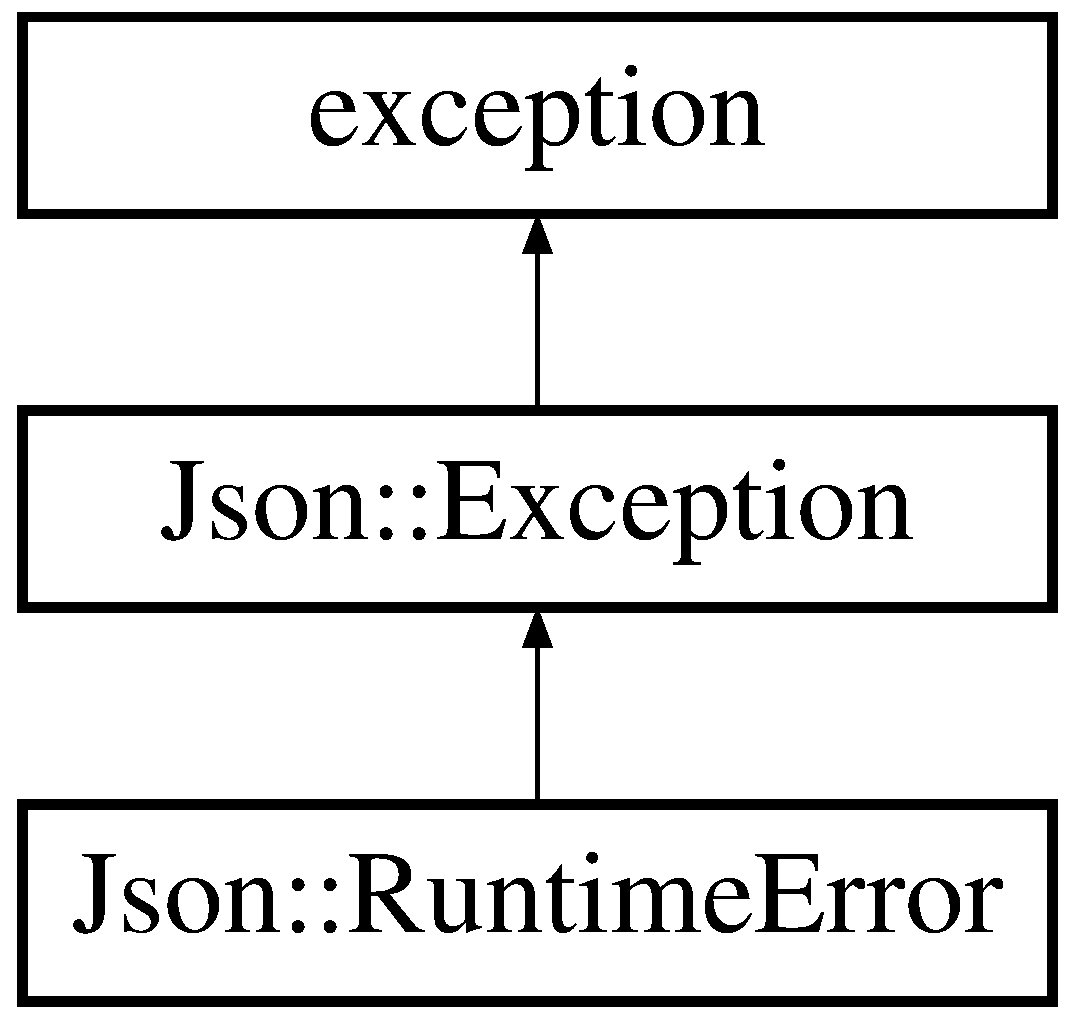
\includegraphics[height=3.000000cm]{classJson_1_1RuntimeError}
\end{center}
\end{figure}
\subsection*{Public Member Functions}
\begin{DoxyCompactItemize}
\item 
\hyperlink{classJson_1_1RuntimeError_a0f6445dc345ce0a703610b6e893fee40_a0f6445dc345ce0a703610b6e893fee40}{Runtime\+Error} (\hyperlink{json_8h_a1e723f95759de062585bc4a8fd3fa4be_a1e723f95759de062585bc4a8fd3fa4be}{J\+S\+O\+N\+C\+P\+P\+\_\+\+S\+T\+R\+I\+NG} const \&msg)
\end{DoxyCompactItemize}
\subsection*{Additional Inherited Members}


\subsection{Detailed Description}
Exceptions which the user cannot easily avoid.

E.\+g. out-\/of-\/memory (when we use malloc), stack-\/overflow, malicious input

\begin{DoxyRemark}{Remarks}
derived from \hyperlink{classJson_1_1Exception}{Json\+::\+Exception} 
\end{DoxyRemark}


\subsection{Constructor \& Destructor Documentation}
\mbox{\Hypertarget{classJson_1_1RuntimeError_a0f6445dc345ce0a703610b6e893fee40_a0f6445dc345ce0a703610b6e893fee40}\label{classJson_1_1RuntimeError_a0f6445dc345ce0a703610b6e893fee40_a0f6445dc345ce0a703610b6e893fee40}} 
\index{Json\+::\+Runtime\+Error@{Json\+::\+Runtime\+Error}!Runtime\+Error@{Runtime\+Error}}
\index{Runtime\+Error@{Runtime\+Error}!Json\+::\+Runtime\+Error@{Json\+::\+Runtime\+Error}}
\subsubsection{\texorpdfstring{Runtime\+Error()}{RuntimeError()}}
{\footnotesize\ttfamily Json\+::\+Runtime\+Error\+::\+Runtime\+Error (\begin{DoxyParamCaption}\item[{\hyperlink{json_8h_a1e723f95759de062585bc4a8fd3fa4be_a1e723f95759de062585bc4a8fd3fa4be}{J\+S\+O\+N\+C\+P\+P\+\_\+\+S\+T\+R\+I\+NG} const \&}]{msg }\end{DoxyParamCaption})}



The documentation for this class was generated from the following files\+:\begin{DoxyCompactItemize}
\item 
json/\hyperlink{json_8h}{json.\+h}\item 
\hyperlink{jsoncpp_8cpp}{jsoncpp.\+cpp}\end{DoxyCompactItemize}

\hypertarget{unionsocket__address}{}\section{socket\+\_\+address Union Reference}
\label{unionsocket__address}\index{socket\+\_\+address@{socket\+\_\+address}}
\subsection*{Public Attributes}
\begin{DoxyCompactItemize}
\item 
\mbox{\Hypertarget{unionsocket__address_ab6a9b0bc545e839df7e06e5b6bff0891}\label{unionsocket__address_ab6a9b0bc545e839df7e06e5b6bff0891}} 
struct sockaddr {\bfseries sa}
\item 
\mbox{\Hypertarget{unionsocket__address_af540a7224ea459c48bc6ec1ca592e55d}\label{unionsocket__address_af540a7224ea459c48bc6ec1ca592e55d}} 
struct sockaddr\+\_\+in {\bfseries sin}
\item 
\mbox{\Hypertarget{unionsocket__address_a923a2caba3cad046553b3632f7c2c571}\label{unionsocket__address_a923a2caba3cad046553b3632f7c2c571}} 
struct sockaddr {\bfseries sin6}
\end{DoxyCompactItemize}


The documentation for this union was generated from the following file\+:\begin{DoxyCompactItemize}
\item 
mongoose.\+h\end{DoxyCompactItemize}

\hypertarget{classJson_1_1StaticString}{}\section{Json\+:\+:Static\+String Class Reference}
\label{classJson_1_1StaticString}\index{Json\+::\+Static\+String@{Json\+::\+Static\+String}}


Lightweight wrapper to tag static string.  




{\ttfamily \#include $<$json.\+h$>$}

\subsection*{Public Member Functions}
\begin{DoxyCompactItemize}
\item 
\hyperlink{classJson_1_1StaticString_afb6baf1ec078ce76f0b0f9b39d19437f_afb6baf1ec078ce76f0b0f9b39d19437f}{Static\+String} (const char $\ast$czstring)
\item 
\hyperlink{classJson_1_1StaticString_a256a6cc0c630aef670848a0f11707b62_a256a6cc0c630aef670848a0f11707b62}{operator const char $\ast$} () const
\item 
const char $\ast$ \hyperlink{classJson_1_1StaticString_ad6be703d432d108623bb0aa06b0b90ca_ad6be703d432d108623bb0aa06b0b90ca}{c\+\_\+str} () const
\end{DoxyCompactItemize}
\subsection*{Private Attributes}
\begin{DoxyCompactItemize}
\item 
const char $\ast$ \hyperlink{classJson_1_1StaticString_a9f0d9e8caee8f8db14e2c8c24760dffd_a9f0d9e8caee8f8db14e2c8c24760dffd}{c\+\_\+str\+\_\+}
\end{DoxyCompactItemize}


\subsection{Detailed Description}
Lightweight wrapper to tag static string. 

\hyperlink{classJson_1_1Value}{Value} constructor and object\+Value member assignement takes advantage of the \hyperlink{classJson_1_1StaticString}{Static\+String} and avoid the cost of string duplication when storing the string or the member name.

Example of usage\+: 
\begin{DoxyCode}
\hyperlink{classJson_1_1Value}{Json::Value} aValue( \hyperlink{classJson_1_1StaticString_afb6baf1ec078ce76f0b0f9b39d19437f_afb6baf1ec078ce76f0b0f9b39d19437f}{StaticString}(\textcolor{stringliteral}{"some text"}) );
\hyperlink{classJson_1_1Value}{Json::Value} object;
\textcolor{keyword}{static} \textcolor{keyword}{const} \hyperlink{classJson_1_1StaticString_afb6baf1ec078ce76f0b0f9b39d19437f_afb6baf1ec078ce76f0b0f9b39d19437f}{StaticString} code(\textcolor{stringliteral}{"code"});
\textcolor{keywordtype}{object}[code] = 1234;
\end{DoxyCode}
 

\subsection{Constructor \& Destructor Documentation}
\mbox{\Hypertarget{classJson_1_1StaticString_afb6baf1ec078ce76f0b0f9b39d19437f_afb6baf1ec078ce76f0b0f9b39d19437f}\label{classJson_1_1StaticString_afb6baf1ec078ce76f0b0f9b39d19437f_afb6baf1ec078ce76f0b0f9b39d19437f}} 
\index{Json\+::\+Static\+String@{Json\+::\+Static\+String}!Static\+String@{Static\+String}}
\index{Static\+String@{Static\+String}!Json\+::\+Static\+String@{Json\+::\+Static\+String}}
\subsubsection{\texorpdfstring{Static\+String()}{StaticString()}}
{\footnotesize\ttfamily Json\+::\+Static\+String\+::\+Static\+String (\begin{DoxyParamCaption}\item[{const char $\ast$}]{czstring }\end{DoxyParamCaption})\hspace{0.3cm}{\ttfamily [inline]}, {\ttfamily [explicit]}}



\subsection{Member Function Documentation}
\mbox{\Hypertarget{classJson_1_1StaticString_ad6be703d432d108623bb0aa06b0b90ca_ad6be703d432d108623bb0aa06b0b90ca}\label{classJson_1_1StaticString_ad6be703d432d108623bb0aa06b0b90ca_ad6be703d432d108623bb0aa06b0b90ca}} 
\index{Json\+::\+Static\+String@{Json\+::\+Static\+String}!c\+\_\+str@{c\+\_\+str}}
\index{c\+\_\+str@{c\+\_\+str}!Json\+::\+Static\+String@{Json\+::\+Static\+String}}
\subsubsection{\texorpdfstring{c\+\_\+str()}{c\_str()}}
{\footnotesize\ttfamily const char$\ast$ Json\+::\+Static\+String\+::c\+\_\+str (\begin{DoxyParamCaption}{ }\end{DoxyParamCaption}) const\hspace{0.3cm}{\ttfamily [inline]}}



Referenced by Json\+::\+Value\+::operator\mbox{[}$\,$\mbox{]}(), and Json\+::\+Value\+::\+Value().

\mbox{\Hypertarget{classJson_1_1StaticString_a256a6cc0c630aef670848a0f11707b62_a256a6cc0c630aef670848a0f11707b62}\label{classJson_1_1StaticString_a256a6cc0c630aef670848a0f11707b62_a256a6cc0c630aef670848a0f11707b62}} 
\index{Json\+::\+Static\+String@{Json\+::\+Static\+String}!operator const char $\ast$@{operator const char $\ast$}}
\index{operator const char $\ast$@{operator const char $\ast$}!Json\+::\+Static\+String@{Json\+::\+Static\+String}}
\subsubsection{\texorpdfstring{operator const char $\ast$()}{operator const char *()}}
{\footnotesize\ttfamily Json\+::\+Static\+String\+::operator const char $\ast$ (\begin{DoxyParamCaption}{ }\end{DoxyParamCaption}) const\hspace{0.3cm}{\ttfamily [inline]}}



\subsection{Member Data Documentation}
\mbox{\Hypertarget{classJson_1_1StaticString_a9f0d9e8caee8f8db14e2c8c24760dffd_a9f0d9e8caee8f8db14e2c8c24760dffd}\label{classJson_1_1StaticString_a9f0d9e8caee8f8db14e2c8c24760dffd_a9f0d9e8caee8f8db14e2c8c24760dffd}} 
\index{Json\+::\+Static\+String@{Json\+::\+Static\+String}!c\+\_\+str\+\_\+@{c\+\_\+str\+\_\+}}
\index{c\+\_\+str\+\_\+@{c\+\_\+str\+\_\+}!Json\+::\+Static\+String@{Json\+::\+Static\+String}}
\subsubsection{\texorpdfstring{c\+\_\+str\+\_\+}{c\_str\_}}
{\footnotesize\ttfamily const char$\ast$ Json\+::\+Static\+String\+::c\+\_\+str\+\_\+\hspace{0.3cm}{\ttfamily [private]}}



The documentation for this class was generated from the following file\+:\begin{DoxyCompactItemize}
\item 
json/\hyperlink{json_8h}{json.\+h}\end{DoxyCompactItemize}

\hypertarget{classJson_1_1StreamWriter}{}\section{Json\+:\+:Stream\+Writer Class Reference}
\label{classJson_1_1StreamWriter}\index{Json\+::\+Stream\+Writer@{Json\+::\+Stream\+Writer}}


{\ttfamily \#include $<$json.\+h$>$}

Inheritance diagram for Json\+:\+:Stream\+Writer\+:\begin{figure}[H]
\begin{center}
\leavevmode
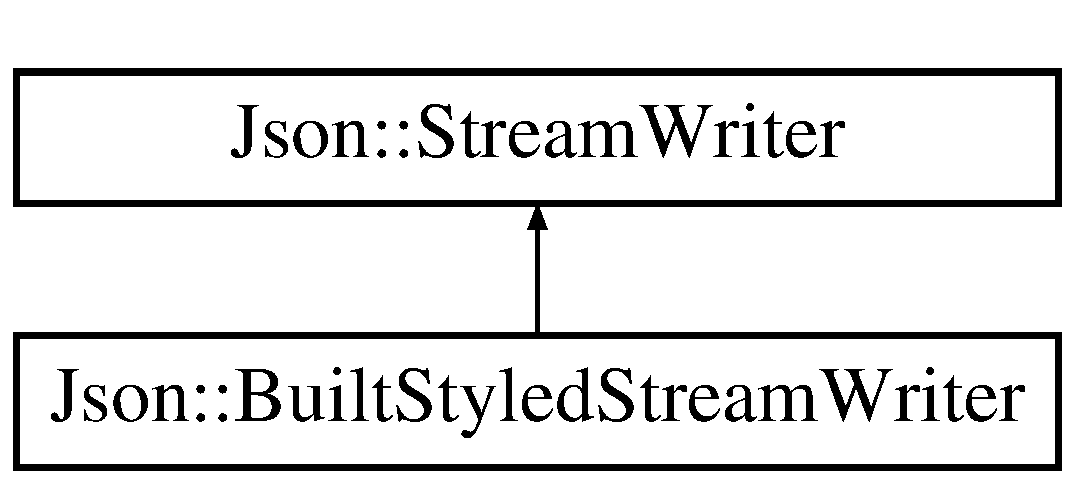
\includegraphics[height=2.000000cm]{classJson_1_1StreamWriter}
\end{center}
\end{figure}
\subsection*{Classes}
\begin{DoxyCompactItemize}
\item 
class \hyperlink{classJson_1_1StreamWriter_1_1Factory}{Factory}
\begin{DoxyCompactList}\small\item\em A simple abstract factory. \end{DoxyCompactList}\end{DoxyCompactItemize}
\subsection*{Public Member Functions}
\begin{DoxyCompactItemize}
\item 
\hyperlink{classJson_1_1StreamWriter_a66e6f5113618ce6b04cac9b3c85a3707_a66e6f5113618ce6b04cac9b3c85a3707}{Stream\+Writer} ()
\item 
virtual \hyperlink{classJson_1_1StreamWriter_a03f8fb6a873b6b50f05bc4556e043c3a_a03f8fb6a873b6b50f05bc4556e043c3a}{$\sim$\+Stream\+Writer} ()
\item 
virtual int \hyperlink{classJson_1_1StreamWriter_a84278bad0c9a9fc587bc2a97c5bb5993_a84278bad0c9a9fc587bc2a97c5bb5993}{write} (\hyperlink{classJson_1_1Value}{Value} const \&root, \hyperlink{json_8h_a37a25be5fca174927780caeb280094ce_a37a25be5fca174927780caeb280094ce}{J\+S\+O\+N\+C\+P\+P\+\_\+\+O\+S\+T\+R\+E\+AM} $\ast$sout)=0
\end{DoxyCompactItemize}
\subsection*{Protected Attributes}
\begin{DoxyCompactItemize}
\item 
\hyperlink{json_8h_a37a25be5fca174927780caeb280094ce_a37a25be5fca174927780caeb280094ce}{J\+S\+O\+N\+C\+P\+P\+\_\+\+O\+S\+T\+R\+E\+AM} $\ast$ \hyperlink{classJson_1_1StreamWriter_a4f5603d4228a9fa46a42cb44e5234d9b_a4f5603d4228a9fa46a42cb44e5234d9b}{sout\+\_\+}
\end{DoxyCompactItemize}


\subsection{Detailed Description}
Usage\+: 
\begin{DoxyCode}
\textcolor{keyword}{using namespace }\hyperlink{namespaceJson}{Json};
\textcolor{keywordtype}{void} writeToStdout(\hyperlink{classJson_1_1StreamWriter_1_1Factory}{StreamWriter::Factory} \textcolor{keyword}{const}& factory, 
      \hyperlink{classJson_1_1Value}{Value} \textcolor{keyword}{const}& value) \{
  std::unique\_ptr<StreamWriter> \textcolor{keyword}{const} writer(
    factory.\hyperlink{classJson_1_1StreamWriter_1_1Factory_a9d30ec53e8288cd53befccf1009c5f31_a9d30ec53e8288cd53befccf1009c5f31}{newStreamWriter}());
  writer->write(value, &std::cout);
  std::cout << std::endl;  \textcolor{comment}{// add lf and flush}
\}
\end{DoxyCode}
 

\subsection{Constructor \& Destructor Documentation}
\mbox{\Hypertarget{classJson_1_1StreamWriter_a66e6f5113618ce6b04cac9b3c85a3707_a66e6f5113618ce6b04cac9b3c85a3707}\label{classJson_1_1StreamWriter_a66e6f5113618ce6b04cac9b3c85a3707_a66e6f5113618ce6b04cac9b3c85a3707}} 
\index{Json\+::\+Stream\+Writer@{Json\+::\+Stream\+Writer}!Stream\+Writer@{Stream\+Writer}}
\index{Stream\+Writer@{Stream\+Writer}!Json\+::\+Stream\+Writer@{Json\+::\+Stream\+Writer}}
\subsubsection{\texorpdfstring{Stream\+Writer()}{StreamWriter()}}
{\footnotesize\ttfamily Json\+::\+Stream\+Writer\+::\+Stream\+Writer (\begin{DoxyParamCaption}{ }\end{DoxyParamCaption})}

\mbox{\Hypertarget{classJson_1_1StreamWriter_a03f8fb6a873b6b50f05bc4556e043c3a_a03f8fb6a873b6b50f05bc4556e043c3a}\label{classJson_1_1StreamWriter_a03f8fb6a873b6b50f05bc4556e043c3a_a03f8fb6a873b6b50f05bc4556e043c3a}} 
\index{Json\+::\+Stream\+Writer@{Json\+::\+Stream\+Writer}!````~Stream\+Writer@{$\sim$\+Stream\+Writer}}
\index{````~Stream\+Writer@{$\sim$\+Stream\+Writer}!Json\+::\+Stream\+Writer@{Json\+::\+Stream\+Writer}}
\subsubsection{\texorpdfstring{$\sim$\+Stream\+Writer()}{~StreamWriter()}}
{\footnotesize\ttfamily Json\+::\+Stream\+Writer\+::$\sim$\+Stream\+Writer (\begin{DoxyParamCaption}{ }\end{DoxyParamCaption})\hspace{0.3cm}{\ttfamily [virtual]}}



\subsection{Member Function Documentation}
\mbox{\Hypertarget{classJson_1_1StreamWriter_a84278bad0c9a9fc587bc2a97c5bb5993_a84278bad0c9a9fc587bc2a97c5bb5993}\label{classJson_1_1StreamWriter_a84278bad0c9a9fc587bc2a97c5bb5993_a84278bad0c9a9fc587bc2a97c5bb5993}} 
\index{Json\+::\+Stream\+Writer@{Json\+::\+Stream\+Writer}!write@{write}}
\index{write@{write}!Json\+::\+Stream\+Writer@{Json\+::\+Stream\+Writer}}
\subsubsection{\texorpdfstring{write()}{write()}}
{\footnotesize\ttfamily virtual int Json\+::\+Stream\+Writer\+::write (\begin{DoxyParamCaption}\item[{\hyperlink{classJson_1_1Value}{Value} const \&}]{root,  }\item[{\hyperlink{json_8h_a37a25be5fca174927780caeb280094ce_a37a25be5fca174927780caeb280094ce}{J\+S\+O\+N\+C\+P\+P\+\_\+\+O\+S\+T\+R\+E\+AM} $\ast$}]{sout }\end{DoxyParamCaption})\hspace{0.3cm}{\ttfamily [pure virtual]}}

Write \hyperlink{classJson_1_1Value}{Value} into document as configured in sub-\/class. Do not take ownership of sout, but maintain a reference during function. \begin{DoxyPrecond}{Precondition}
sout != N\+U\+LL 
\end{DoxyPrecond}
\begin{DoxyReturn}{Returns}
zero on success (For now, we always return zero, so check the stream instead.) 
\end{DoxyReturn}

\begin{DoxyExceptions}{Exceptions}
{\em std\+::exception} & possibly, depending on configuration \\
\hline
\end{DoxyExceptions}


Implemented in \hyperlink{structJson_1_1BuiltStyledStreamWriter_a823cdb1afabb6b0d5f39bcd5a6a6f747_a823cdb1afabb6b0d5f39bcd5a6a6f747}{Json\+::\+Built\+Styled\+Stream\+Writer}.



\subsection{Member Data Documentation}
\mbox{\Hypertarget{classJson_1_1StreamWriter_a4f5603d4228a9fa46a42cb44e5234d9b_a4f5603d4228a9fa46a42cb44e5234d9b}\label{classJson_1_1StreamWriter_a4f5603d4228a9fa46a42cb44e5234d9b_a4f5603d4228a9fa46a42cb44e5234d9b}} 
\index{Json\+::\+Stream\+Writer@{Json\+::\+Stream\+Writer}!sout\+\_\+@{sout\+\_\+}}
\index{sout\+\_\+@{sout\+\_\+}!Json\+::\+Stream\+Writer@{Json\+::\+Stream\+Writer}}
\subsubsection{\texorpdfstring{sout\+\_\+}{sout\_}}
{\footnotesize\ttfamily \hyperlink{json_8h_a37a25be5fca174927780caeb280094ce_a37a25be5fca174927780caeb280094ce}{J\+S\+O\+N\+C\+P\+P\+\_\+\+O\+S\+T\+R\+E\+AM}$\ast$ Json\+::\+Stream\+Writer\+::sout\+\_\+\hspace{0.3cm}{\ttfamily [protected]}}



Referenced by Json\+::\+Built\+Styled\+Stream\+Writer\+::push\+Value(), Json\+::\+Built\+Styled\+Stream\+Writer\+::write(), Json\+::\+Built\+Styled\+Stream\+Writer\+::write\+Array\+Value(), Json\+::\+Built\+Styled\+Stream\+Writer\+::write\+Comment\+After\+Value\+On\+Same\+Line(), Json\+::\+Built\+Styled\+Stream\+Writer\+::write\+Comment\+Before\+Value(), Json\+::\+Built\+Styled\+Stream\+Writer\+::write\+Indent(), Json\+::\+Built\+Styled\+Stream\+Writer\+::write\+Value(), and Json\+::\+Built\+Styled\+Stream\+Writer\+::write\+With\+Indent().



The documentation for this class was generated from the following files\+:\begin{DoxyCompactItemize}
\item 
json/\hyperlink{json_8h}{json.\+h}\item 
\hyperlink{jsoncpp_8cpp}{jsoncpp.\+cpp}\end{DoxyCompactItemize}

\hypertarget{classJson_1_1StreamWriterBuilder}{}\section{Json\+:\+:Stream\+Writer\+Builder Class Reference}
\label{classJson_1_1StreamWriterBuilder}\index{Json\+::\+Stream\+Writer\+Builder@{Json\+::\+Stream\+Writer\+Builder}}


Build a \hyperlink{classJson_1_1StreamWriter}{Stream\+Writer} implementation.  




{\ttfamily \#include $<$json.\+h$>$}

Inheritance diagram for Json\+:\+:Stream\+Writer\+Builder\+:\begin{figure}[H]
\begin{center}
\leavevmode
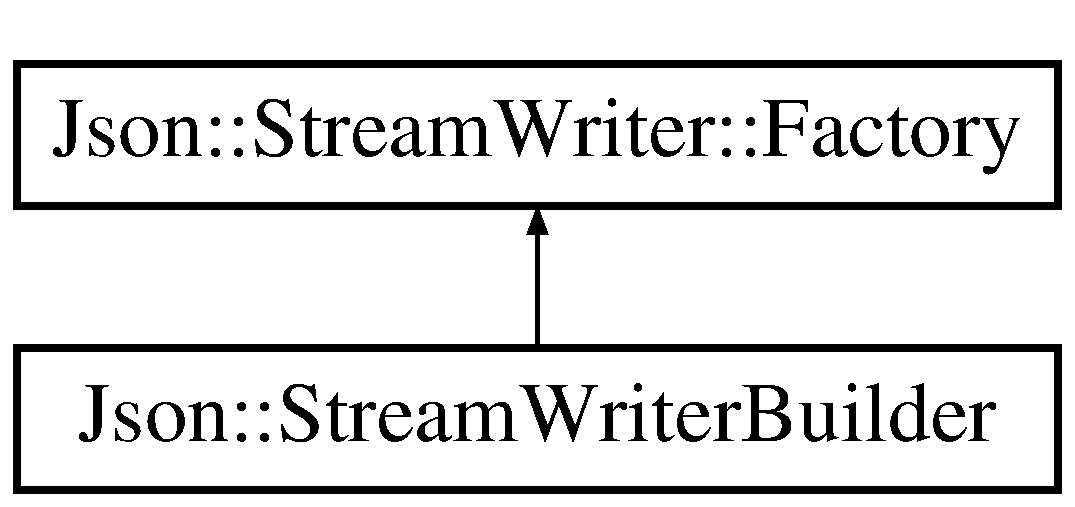
\includegraphics[height=2.000000cm]{classJson_1_1StreamWriterBuilder}
\end{center}
\end{figure}
\subsection*{Public Member Functions}
\begin{DoxyCompactItemize}
\item 
\hyperlink{classJson_1_1StreamWriterBuilder_ab95b76179c152673ad14abc639a46ee4_ab95b76179c152673ad14abc639a46ee4}{Stream\+Writer\+Builder} ()
\item 
\hyperlink{classJson_1_1StreamWriterBuilder_a93263f8ef1e2d22593907075d8f0aaef_a93263f8ef1e2d22593907075d8f0aaef}{$\sim$\+Stream\+Writer\+Builder} () \hyperlink{json_8h_a824d6199c91488107e443226fa6022c5_a824d6199c91488107e443226fa6022c5}{J\+S\+O\+N\+C\+P\+P\+\_\+\+O\+V\+E\+R\+R\+I\+DE}
\item 
\hyperlink{classJson_1_1StreamWriter}{Stream\+Writer} $\ast$ \hyperlink{classJson_1_1StreamWriterBuilder_ab9ee278609f88ae04a7c1a84e1f559e6_ab9ee278609f88ae04a7c1a84e1f559e6}{new\+Stream\+Writer} () const \hyperlink{json_8h_a824d6199c91488107e443226fa6022c5_a824d6199c91488107e443226fa6022c5}{J\+S\+O\+N\+C\+P\+P\+\_\+\+O\+V\+E\+R\+R\+I\+DE}
\item 
bool \hyperlink{classJson_1_1StreamWriterBuilder_a12353b97766841db7d049da84658da09_a12353b97766841db7d049da84658da09}{validate} (\hyperlink{classJson_1_1Value}{Json\+::\+Value} $\ast$invalid) const
\item 
\hyperlink{classJson_1_1Value}{Value} \& \hyperlink{classJson_1_1StreamWriterBuilder_af68f6b59cb20b074052ed12bb3d336a3_af68f6b59cb20b074052ed12bb3d336a3}{operator\mbox{[}$\,$\mbox{]}} (\hyperlink{json_8h_a1e723f95759de062585bc4a8fd3fa4be_a1e723f95759de062585bc4a8fd3fa4be}{J\+S\+O\+N\+C\+P\+P\+\_\+\+S\+T\+R\+I\+NG} key)
\end{DoxyCompactItemize}
\subsection*{Static Public Member Functions}
\begin{DoxyCompactItemize}
\item 
static void \hyperlink{classJson_1_1StreamWriterBuilder_a53bf106b141e28637b01ad0ecd2acbf6_a53bf106b141e28637b01ad0ecd2acbf6}{set\+Defaults} (\hyperlink{classJson_1_1Value}{Json\+::\+Value} $\ast$settings)
\end{DoxyCompactItemize}
\subsection*{Public Attributes}
\begin{DoxyCompactItemize}
\item 
\hyperlink{classJson_1_1Value}{Json\+::\+Value} \hyperlink{classJson_1_1StreamWriterBuilder_a79bdf2e639a52f4e758c0b95bd1d3423_a79bdf2e639a52f4e758c0b95bd1d3423}{settings\+\_\+}
\end{DoxyCompactItemize}


\subsection{Detailed Description}
Build a \hyperlink{classJson_1_1StreamWriter}{Stream\+Writer} implementation. 

Usage\+: 
\begin{DoxyCode}
\textcolor{keyword}{using namespace }\hyperlink{namespaceJson}{Json};
\hyperlink{classJson_1_1Value}{Value} value = ...;
\hyperlink{classJson_1_1StreamWriterBuilder}{StreamWriterBuilder} builder;
builder[\textcolor{stringliteral}{"commentStyle"}] = \textcolor{stringliteral}{"None"};
builder[\textcolor{stringliteral}{"indentation"}] = \textcolor{stringliteral}{"   "};  \textcolor{comment}{// or whatever you like}
std::unique\_ptr<Json::StreamWriter> writer(
    builder.\hyperlink{classJson_1_1StreamWriterBuilder_ab9ee278609f88ae04a7c1a84e1f559e6_ab9ee278609f88ae04a7c1a84e1f559e6}{newStreamWriter}());
writer->write(value, &std::cout);
std::cout << std::endl;  \textcolor{comment}{// add lf and flush}
\end{DoxyCode}
 

\subsection{Constructor \& Destructor Documentation}
\mbox{\Hypertarget{classJson_1_1StreamWriterBuilder_ab95b76179c152673ad14abc639a46ee4_ab95b76179c152673ad14abc639a46ee4}\label{classJson_1_1StreamWriterBuilder_ab95b76179c152673ad14abc639a46ee4_ab95b76179c152673ad14abc639a46ee4}} 
\index{Json\+::\+Stream\+Writer\+Builder@{Json\+::\+Stream\+Writer\+Builder}!Stream\+Writer\+Builder@{Stream\+Writer\+Builder}}
\index{Stream\+Writer\+Builder@{Stream\+Writer\+Builder}!Json\+::\+Stream\+Writer\+Builder@{Json\+::\+Stream\+Writer\+Builder}}
\subsubsection{\texorpdfstring{Stream\+Writer\+Builder()}{StreamWriterBuilder()}}
{\footnotesize\ttfamily Json\+::\+Stream\+Writer\+Builder\+::\+Stream\+Writer\+Builder (\begin{DoxyParamCaption}{ }\end{DoxyParamCaption})}

\mbox{\Hypertarget{classJson_1_1StreamWriterBuilder_a93263f8ef1e2d22593907075d8f0aaef_a93263f8ef1e2d22593907075d8f0aaef}\label{classJson_1_1StreamWriterBuilder_a93263f8ef1e2d22593907075d8f0aaef_a93263f8ef1e2d22593907075d8f0aaef}} 
\index{Json\+::\+Stream\+Writer\+Builder@{Json\+::\+Stream\+Writer\+Builder}!````~Stream\+Writer\+Builder@{$\sim$\+Stream\+Writer\+Builder}}
\index{````~Stream\+Writer\+Builder@{$\sim$\+Stream\+Writer\+Builder}!Json\+::\+Stream\+Writer\+Builder@{Json\+::\+Stream\+Writer\+Builder}}
\subsubsection{\texorpdfstring{$\sim$\+Stream\+Writer\+Builder()}{~StreamWriterBuilder()}}
{\footnotesize\ttfamily Json\+::\+Stream\+Writer\+Builder\+::$\sim$\+Stream\+Writer\+Builder (\begin{DoxyParamCaption}{ }\end{DoxyParamCaption})}



\subsection{Member Function Documentation}
\mbox{\Hypertarget{classJson_1_1StreamWriterBuilder_ab9ee278609f88ae04a7c1a84e1f559e6_ab9ee278609f88ae04a7c1a84e1f559e6}\label{classJson_1_1StreamWriterBuilder_ab9ee278609f88ae04a7c1a84e1f559e6_ab9ee278609f88ae04a7c1a84e1f559e6}} 
\index{Json\+::\+Stream\+Writer\+Builder@{Json\+::\+Stream\+Writer\+Builder}!new\+Stream\+Writer@{new\+Stream\+Writer}}
\index{new\+Stream\+Writer@{new\+Stream\+Writer}!Json\+::\+Stream\+Writer\+Builder@{Json\+::\+Stream\+Writer\+Builder}}
\subsubsection{\texorpdfstring{new\+Stream\+Writer()}{newStreamWriter()}}
{\footnotesize\ttfamily \hyperlink{classJson_1_1StreamWriter}{Stream\+Writer} $\ast$ Json\+::\+Stream\+Writer\+Builder\+::new\+Stream\+Writer (\begin{DoxyParamCaption}{ }\end{DoxyParamCaption}) const\hspace{0.3cm}{\ttfamily [virtual]}}


\begin{DoxyExceptions}{Exceptions}
{\em std\+::exception} & if something goes wrong (e.\+g. invalid settings) \\
\hline
\end{DoxyExceptions}


Implements \hyperlink{classJson_1_1StreamWriter_1_1Factory_a9d30ec53e8288cd53befccf1009c5f31_a9d30ec53e8288cd53befccf1009c5f31}{Json\+::\+Stream\+Writer\+::\+Factory}.



References Json\+::\+Comment\+Style\+::\+All, J\+S\+O\+N\+C\+P\+P\+\_\+\+S\+T\+R\+I\+NG, Json\+::\+Comment\+Style\+::\+None, and Json\+::throw\+Runtime\+Error().



Referenced by Json\+::operator$<$$<$().

\mbox{\Hypertarget{classJson_1_1StreamWriterBuilder_af68f6b59cb20b074052ed12bb3d336a3_af68f6b59cb20b074052ed12bb3d336a3}\label{classJson_1_1StreamWriterBuilder_af68f6b59cb20b074052ed12bb3d336a3_af68f6b59cb20b074052ed12bb3d336a3}} 
\index{Json\+::\+Stream\+Writer\+Builder@{Json\+::\+Stream\+Writer\+Builder}!operator\mbox{[}\mbox{]}@{operator[]}}
\index{operator\mbox{[}\mbox{]}@{operator[]}!Json\+::\+Stream\+Writer\+Builder@{Json\+::\+Stream\+Writer\+Builder}}
\subsubsection{\texorpdfstring{operator[]()}{operator[]()}}
{\footnotesize\ttfamily \hyperlink{classJson_1_1Value}{Value} \& Json\+::\+Stream\+Writer\+Builder\+::operator\mbox{[}$\,$\mbox{]} (\begin{DoxyParamCaption}\item[{\hyperlink{json_8h_a1e723f95759de062585bc4a8fd3fa4be_a1e723f95759de062585bc4a8fd3fa4be}{J\+S\+O\+N\+C\+P\+P\+\_\+\+S\+T\+R\+I\+NG}}]{key }\end{DoxyParamCaption})}

A simple way to update a specific setting. \mbox{\Hypertarget{classJson_1_1StreamWriterBuilder_a53bf106b141e28637b01ad0ecd2acbf6_a53bf106b141e28637b01ad0ecd2acbf6}\label{classJson_1_1StreamWriterBuilder_a53bf106b141e28637b01ad0ecd2acbf6_a53bf106b141e28637b01ad0ecd2acbf6}} 
\index{Json\+::\+Stream\+Writer\+Builder@{Json\+::\+Stream\+Writer\+Builder}!set\+Defaults@{set\+Defaults}}
\index{set\+Defaults@{set\+Defaults}!Json\+::\+Stream\+Writer\+Builder@{Json\+::\+Stream\+Writer\+Builder}}
\subsubsection{\texorpdfstring{set\+Defaults()}{setDefaults()}}
{\footnotesize\ttfamily void Json\+::\+Stream\+Writer\+Builder\+::set\+Defaults (\begin{DoxyParamCaption}\item[{\hyperlink{classJson_1_1Value}{Json\+::\+Value} $\ast$}]{settings }\end{DoxyParamCaption})\hspace{0.3cm}{\ttfamily [static]}}

Called by ctor, but you can use this to reset settings\+\_\+. \begin{DoxyPrecond}{Precondition}
\textquotesingle{}settings\textquotesingle{} != N\+U\+LL (but Json\+::null is fine) 
\end{DoxyPrecond}
\begin{DoxyRemark}{Remarks}
Defaults\+: 
\begin{DoxyCodeInclude}
\end{DoxyCodeInclude}

\end{DoxyRemark}
\mbox{[}Stream\+Writer\+Builder\+Defaults\mbox{]}

\mbox{[}Stream\+Writer\+Builder\+Defaults\mbox{]} \mbox{\Hypertarget{classJson_1_1StreamWriterBuilder_a12353b97766841db7d049da84658da09_a12353b97766841db7d049da84658da09}\label{classJson_1_1StreamWriterBuilder_a12353b97766841db7d049da84658da09_a12353b97766841db7d049da84658da09}} 
\index{Json\+::\+Stream\+Writer\+Builder@{Json\+::\+Stream\+Writer\+Builder}!validate@{validate}}
\index{validate@{validate}!Json\+::\+Stream\+Writer\+Builder@{Json\+::\+Stream\+Writer\+Builder}}
\subsubsection{\texorpdfstring{validate()}{validate()}}
{\footnotesize\ttfamily bool Json\+::\+Stream\+Writer\+Builder\+::validate (\begin{DoxyParamCaption}\item[{\hyperlink{classJson_1_1Value}{Json\+::\+Value} $\ast$}]{invalid }\end{DoxyParamCaption}) const}

\begin{DoxyReturn}{Returns}
true if \textquotesingle{}settings\textquotesingle{} are legal and consistent; otherwise, indicate bad settings via \textquotesingle{}invalid\textquotesingle{}. 
\end{DoxyReturn}


References Json\+::get\+Valid\+Writer\+Keys(), J\+S\+O\+N\+C\+P\+P\+\_\+\+S\+T\+R\+I\+NG, and Json\+::\+Value\+::size().



\subsection{Member Data Documentation}
\mbox{\Hypertarget{classJson_1_1StreamWriterBuilder_a79bdf2e639a52f4e758c0b95bd1d3423_a79bdf2e639a52f4e758c0b95bd1d3423}\label{classJson_1_1StreamWriterBuilder_a79bdf2e639a52f4e758c0b95bd1d3423_a79bdf2e639a52f4e758c0b95bd1d3423}} 
\index{Json\+::\+Stream\+Writer\+Builder@{Json\+::\+Stream\+Writer\+Builder}!settings\+\_\+@{settings\+\_\+}}
\index{settings\+\_\+@{settings\+\_\+}!Json\+::\+Stream\+Writer\+Builder@{Json\+::\+Stream\+Writer\+Builder}}
\subsubsection{\texorpdfstring{settings\+\_\+}{settings\_}}
{\footnotesize\ttfamily \hyperlink{classJson_1_1Value}{Json\+::\+Value} Json\+::\+Stream\+Writer\+Builder\+::settings\+\_\+}

Configuration of this builder. Available settings (case-\/sensitive)\+:
\begin{DoxyItemize}
\item \char`\"{}comment\+Style\char`\"{}\+: \char`\"{}\+None\char`\"{} or \char`\"{}\+All\char`\"{}
\item \char`\"{}indentation\char`\"{}\+: \char`\"{}$<$anything$>$\char`\"{}
\item \char`\"{}enable\+Y\+A\+M\+L\+Compatibility\char`\"{}\+: false or true
\begin{DoxyItemize}
\item slightly change the whitespace around colons
\end{DoxyItemize}
\item \char`\"{}drop\+Null\+Placeholders\char`\"{}\+: false or true
\begin{DoxyItemize}
\item Drop the \char`\"{}null\char`\"{} string from the writer\textquotesingle{}s output for null\+Values. Strictly speaking, this is not valid J\+S\+ON. But when the output is being fed to a browser\textquotesingle{}s Javascript, it makes for smaller output and the browser can handle the output just fine.
\end{DoxyItemize}
\item \char`\"{}use\+Special\+Floats\char`\"{}\+: false or true
\begin{DoxyItemize}
\item If true, outputs non-\/finite floating point values in the following way\+: NaN values as \char`\"{}\+Na\+N\char`\"{}, positive infinity as \char`\"{}\+Infinity\char`\"{}, and negative infinity as \char`\"{}-\/\+Infinity\char`\"{}.
\end{DoxyItemize}
\end{DoxyItemize}

You can examine \textquotesingle{}settings\+\_\+` yourself to see the defaults. You can also write and read them just like any J\+S\+ON \hyperlink{classJson_1_1Value}{Value}. \begin{DoxySeeAlso}{See also}
\hyperlink{classJson_1_1StreamWriterBuilder_a53bf106b141e28637b01ad0ecd2acbf6_a53bf106b141e28637b01ad0ecd2acbf6}{set\+Defaults()} 
\end{DoxySeeAlso}


The documentation for this class was generated from the following files\+:\begin{DoxyCompactItemize}
\item 
json/\hyperlink{json_8h}{json.\+h}\item 
\hyperlink{jsoncpp_8cpp}{jsoncpp.\+cpp}\end{DoxyCompactItemize}

\hypertarget{structJson_1_1OurReader_1_1StructuredError}{}\section{Json\+:\+:Our\+Reader\+:\+:Structured\+Error Struct Reference}
\label{structJson_1_1OurReader_1_1StructuredError}\index{Json\+::\+Our\+Reader\+::\+Structured\+Error@{Json\+::\+Our\+Reader\+::\+Structured\+Error}}
\subsection*{Public Attributes}
\begin{DoxyCompactItemize}
\item 
ptrdiff\+\_\+t \hyperlink{structJson_1_1OurReader_1_1StructuredError_a102677698afb8177c985e72dafe72b15_a102677698afb8177c985e72dafe72b15}{offset\+\_\+start}
\item 
ptrdiff\+\_\+t \hyperlink{structJson_1_1OurReader_1_1StructuredError_a15491a751a39c5153af04e68b1d0abb9_a15491a751a39c5153af04e68b1d0abb9}{offset\+\_\+limit}
\item 
\hyperlink{json_8h_a1e723f95759de062585bc4a8fd3fa4be_a1e723f95759de062585bc4a8fd3fa4be}{J\+S\+O\+N\+C\+P\+P\+\_\+\+S\+T\+R\+I\+NG} \hyperlink{structJson_1_1OurReader_1_1StructuredError_a9d0b9986bf765d067dfcf2f971a450d1_a9d0b9986bf765d067dfcf2f971a450d1}{message}
\end{DoxyCompactItemize}


\subsection{Member Data Documentation}
\mbox{\Hypertarget{structJson_1_1OurReader_1_1StructuredError_a9d0b9986bf765d067dfcf2f971a450d1_a9d0b9986bf765d067dfcf2f971a450d1}\label{structJson_1_1OurReader_1_1StructuredError_a9d0b9986bf765d067dfcf2f971a450d1_a9d0b9986bf765d067dfcf2f971a450d1}} 
\index{Json\+::\+Our\+Reader\+::\+Structured\+Error@{Json\+::\+Our\+Reader\+::\+Structured\+Error}!message@{message}}
\index{message@{message}!Json\+::\+Our\+Reader\+::\+Structured\+Error@{Json\+::\+Our\+Reader\+::\+Structured\+Error}}
\subsubsection{\texorpdfstring{message}{message}}
{\footnotesize\ttfamily \hyperlink{json_8h_a1e723f95759de062585bc4a8fd3fa4be_a1e723f95759de062585bc4a8fd3fa4be}{J\+S\+O\+N\+C\+P\+P\+\_\+\+S\+T\+R\+I\+NG} Json\+::\+Our\+Reader\+::\+Structured\+Error\+::message}



Referenced by Json\+::\+Our\+Reader\+::get\+Structured\+Errors().

\mbox{\Hypertarget{structJson_1_1OurReader_1_1StructuredError_a15491a751a39c5153af04e68b1d0abb9_a15491a751a39c5153af04e68b1d0abb9}\label{structJson_1_1OurReader_1_1StructuredError_a15491a751a39c5153af04e68b1d0abb9_a15491a751a39c5153af04e68b1d0abb9}} 
\index{Json\+::\+Our\+Reader\+::\+Structured\+Error@{Json\+::\+Our\+Reader\+::\+Structured\+Error}!offset\+\_\+limit@{offset\+\_\+limit}}
\index{offset\+\_\+limit@{offset\+\_\+limit}!Json\+::\+Our\+Reader\+::\+Structured\+Error@{Json\+::\+Our\+Reader\+::\+Structured\+Error}}
\subsubsection{\texorpdfstring{offset\+\_\+limit}{offset\_limit}}
{\footnotesize\ttfamily ptrdiff\+\_\+t Json\+::\+Our\+Reader\+::\+Structured\+Error\+::offset\+\_\+limit}



Referenced by Json\+::\+Our\+Reader\+::get\+Structured\+Errors().

\mbox{\Hypertarget{structJson_1_1OurReader_1_1StructuredError_a102677698afb8177c985e72dafe72b15_a102677698afb8177c985e72dafe72b15}\label{structJson_1_1OurReader_1_1StructuredError_a102677698afb8177c985e72dafe72b15_a102677698afb8177c985e72dafe72b15}} 
\index{Json\+::\+Our\+Reader\+::\+Structured\+Error@{Json\+::\+Our\+Reader\+::\+Structured\+Error}!offset\+\_\+start@{offset\+\_\+start}}
\index{offset\+\_\+start@{offset\+\_\+start}!Json\+::\+Our\+Reader\+::\+Structured\+Error@{Json\+::\+Our\+Reader\+::\+Structured\+Error}}
\subsubsection{\texorpdfstring{offset\+\_\+start}{offset\_start}}
{\footnotesize\ttfamily ptrdiff\+\_\+t Json\+::\+Our\+Reader\+::\+Structured\+Error\+::offset\+\_\+start}



Referenced by Json\+::\+Our\+Reader\+::get\+Structured\+Errors().



The documentation for this struct was generated from the following file\+:\begin{DoxyCompactItemize}
\item 
\hyperlink{jsoncpp_8cpp}{jsoncpp.\+cpp}\end{DoxyCompactItemize}

\hypertarget{structTBT_1_1SystemState}{}\section{T\+BT\+:\+:System\+State Struct Reference}
\label{structTBT_1_1SystemState}\index{T\+B\+T\+::\+System\+State@{T\+B\+T\+::\+System\+State}}
\subsection*{Public Attributes}
\begin{DoxyCompactItemize}
\item 
\mbox{\Hypertarget{structTBT_1_1SystemState_a17d517bed6954e31982eca5685b36d04}\label{structTBT_1_1SystemState_a17d517bed6954e31982eca5685b36d04}} 
uint8\+\_\+t {\bfseries Data\+Len} = 0x14
\item 
\mbox{\Hypertarget{structTBT_1_1SystemState_a27329736b0b53fc4239397b4e9a0194c}\label{structTBT_1_1SystemState_a27329736b0b53fc4239397b4e9a0194c}} 
uint8\+\_\+t {\bfseries filler1} = 0x00
\item 
\mbox{\Hypertarget{structTBT_1_1SystemState_a2a3724acc75f75f94ea6806fb2d0ad1a}\label{structTBT_1_1SystemState_a2a3724acc75f75f94ea6806fb2d0ad1a}} 
uint8\+\_\+t {\bfseries Header} = 0x84
\item 
\mbox{\Hypertarget{structTBT_1_1SystemState_a2dbecb920543f10343d2e13fe0900a6c}\label{structTBT_1_1SystemState_a2dbecb920543f10343d2e13fe0900a6c}} 
uint8\+\_\+t {\bfseries filler2} = 0x00
\item 
\mbox{\Hypertarget{structTBT_1_1SystemState_ad6712d6a9c04e085fd94290b42febf36}\label{structTBT_1_1SystemState_ad6712d6a9c04e085fd94290b42febf36}} 
int16\+\_\+t {\bfseries Main\+Current} = 0x0000
\item 
\mbox{\Hypertarget{structTBT_1_1SystemState_a39dae8a3b2f9789ad770cc1deb6c837b}\label{structTBT_1_1SystemState_a39dae8a3b2f9789ad770cc1deb6c837b}} 
int16\+\_\+t {\bfseries Prog\+Current} = 0x0000
\item 
\mbox{\Hypertarget{structTBT_1_1SystemState_ab1bba48939b28cea2b000bfb7288f1aa}\label{structTBT_1_1SystemState_ab1bba48939b28cea2b000bfb7288f1aa}} 
int16\+\_\+t {\bfseries Filtered\+Main\+Current} = 0x0000
\item 
\mbox{\Hypertarget{structTBT_1_1SystemState_a88b75704f440bbbf3c854bcb6a7d39dc}\label{structTBT_1_1SystemState_a88b75704f440bbbf3c854bcb6a7d39dc}} 
int16\+\_\+t {\bfseries Temperature} = 0x0000
\item 
\mbox{\Hypertarget{structTBT_1_1SystemState_a85f474c9e82ac4f6add54311e7884364}\label{structTBT_1_1SystemState_a85f474c9e82ac4f6add54311e7884364}} 
uint16\+\_\+t {\bfseries Supply\+Voltage} = 0x0000
\item 
\mbox{\Hypertarget{structTBT_1_1SystemState_a29bdf61d0e42828467ecc5e1b7e3c650}\label{structTBT_1_1SystemState_a29bdf61d0e42828467ecc5e1b7e3c650}} 
uint16\+\_\+t {\bfseries V\+C\+C\+Voltage} = 0x0000
\item 
\mbox{\Hypertarget{structTBT_1_1SystemState_afe7823596cb696c8b1f52cdf7f3ee9ef}\label{structTBT_1_1SystemState_afe7823596cb696c8b1f52cdf7f3ee9ef}} 
uint8\+\_\+t {\bfseries Central\+State} = cs\+Track\+Voltage\+Off
\item 
\mbox{\Hypertarget{structTBT_1_1SystemState_a582d67531b086360e8fdd068cf6b2de2}\label{structTBT_1_1SystemState_a582d67531b086360e8fdd068cf6b2de2}} 
uint8\+\_\+t {\bfseries Central\+State\+Ex} = 0x00
\item 
\mbox{\Hypertarget{structTBT_1_1SystemState_abfb73f80485c896dde08ff96122aa087}\label{structTBT_1_1SystemState_abfb73f80485c896dde08ff96122aa087}} 
uint8\+\_\+t {\bfseries reserved1} = 0x00
\item 
\mbox{\Hypertarget{structTBT_1_1SystemState_a43658d0ca2d3eed1df2e0ce3b96861a3}\label{structTBT_1_1SystemState_a43658d0ca2d3eed1df2e0ce3b96861a3}} 
uint8\+\_\+t {\bfseries reserved2} = 0x00
\end{DoxyCompactItemize}


The documentation for this struct was generated from the following file\+:\begin{DoxyCompactItemize}
\item 
Types.\+h\end{DoxyCompactItemize}

\hypertarget{classTBT_1_1UDPClient}{}\section{T\+BT\+:\+:U\+D\+P\+Client Class Reference}
\label{classTBT_1_1UDPClient}\index{T\+B\+T\+::\+U\+D\+P\+Client@{T\+B\+T\+::\+U\+D\+P\+Client}}
Inheritance diagram for T\+BT\+:\+:U\+D\+P\+Client\+:\begin{figure}[H]
\begin{center}
\leavevmode
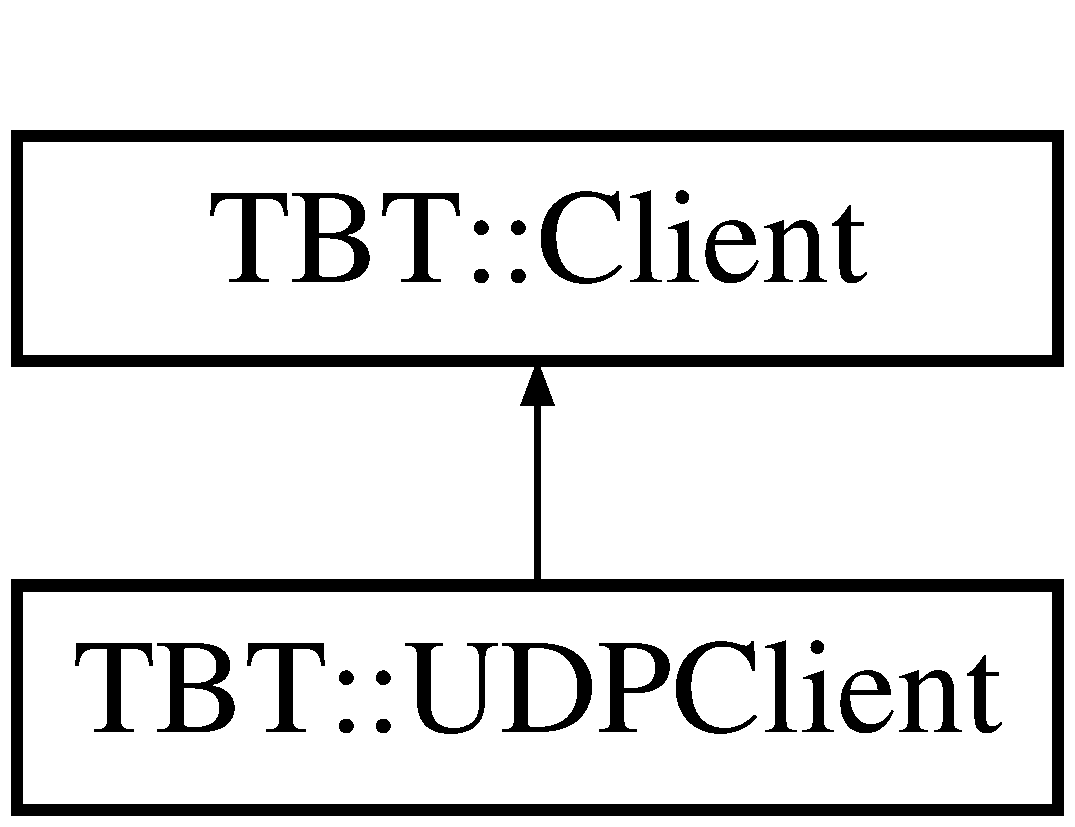
\includegraphics[height=2.000000cm]{classTBT_1_1UDPClient}
\end{center}
\end{figure}
\subsection*{Public Member Functions}
\begin{DoxyCompactItemize}
\item 
\mbox{\Hypertarget{classTBT_1_1UDPClient_a7b6f7858b9d3a7243bdd48fbf150b9f8}\label{classTBT_1_1UDPClient_a7b6f7858b9d3a7243bdd48fbf150b9f8}} 
{\bfseries U\+D\+P\+Client} (\hyperlink{classTBT_1_1UDPClientInterface}{U\+D\+P\+Client\+Interface} $\ast$pinterface, const sockaddr\+\_\+in \&address)
\item 
\mbox{\Hypertarget{classTBT_1_1UDPClient_aaf8b77e98494585ea3c44c9e89ec04ec}\label{classTBT_1_1UDPClient_aaf8b77e98494585ea3c44c9e89ec04ec}} 
virtual void {\bfseries broadcast\+Power\+State\+Change} (Power\+State new\+State)
\item 
\mbox{\Hypertarget{classTBT_1_1UDPClient_a90c650259501f341f531ede72210624a}\label{classTBT_1_1UDPClient_a90c650259501f341f531ede72210624a}} 
virtual void {\bfseries broadcast\+Loc\+Info\+Changed} (\hyperlink{classTBT_1_1LocDecoder}{Loc\+Decoder} $\ast$p\+Loc)
\item 
\mbox{\Hypertarget{classTBT_1_1UDPClient_aad30cea06b570b6a5e688710cfd53100}\label{classTBT_1_1UDPClient_aad30cea06b570b6a5e688710cfd53100}} 
virtual void {\bfseries broadcast\+Emergency\+Stop} (bool state)
\item 
\mbox{\Hypertarget{classTBT_1_1UDPClient_a8471b71655c61bf074b70b62a6dffbf1}\label{classTBT_1_1UDPClient_a8471b71655c61bf074b70b62a6dffbf1}} 
const sockaddr\+\_\+in \& {\bfseries get\+Address} (void)
\item 
\mbox{\Hypertarget{classTBT_1_1UDPClient_a18da0bdc657f707f4c0af6cd3b1e6031}\label{classTBT_1_1UDPClient_a18da0bdc657f707f4c0af6cd3b1e6031}} 
uint32\+\_\+t {\bfseries get\+Broadcast\+Flags} (void)
\item 
\mbox{\Hypertarget{classTBT_1_1UDPClient_a23a0b0ecf47f8a2fe018a570f46ecdfe}\label{classTBT_1_1UDPClient_a23a0b0ecf47f8a2fe018a570f46ecdfe}} 
void {\bfseries set\+Broadcast\+Flags} (uint32\+\_\+t new\+Flags)
\end{DoxyCompactItemize}
\subsection*{Protected Attributes}
\begin{DoxyCompactItemize}
\item 
\mbox{\Hypertarget{classTBT_1_1UDPClient_a880ede9d0208905a251bbfd221646e3b}\label{classTBT_1_1UDPClient_a880ede9d0208905a251bbfd221646e3b}} 
const sockaddr\+\_\+in {\bfseries m\+\_\+\+Address}
\item 
\mbox{\Hypertarget{classTBT_1_1UDPClient_aef66ad83fa20b995152c6f41cb8ba91f}\label{classTBT_1_1UDPClient_aef66ad83fa20b995152c6f41cb8ba91f}} 
int {\bfseries m\+\_\+\+My\+Socket}
\item 
\mbox{\Hypertarget{classTBT_1_1UDPClient_a91eb8f34a9606428eba7230c2bfdb6f6}\label{classTBT_1_1UDPClient_a91eb8f34a9606428eba7230c2bfdb6f6}} 
uint32\+\_\+t {\bfseries m\+\_\+\+Broadcast\+Flags}
\end{DoxyCompactItemize}


The documentation for this class was generated from the following files\+:\begin{DoxyCompactItemize}
\item 
U\+D\+P\+Client.\+h\item 
U\+D\+P\+Client.\+cpp\end{DoxyCompactItemize}

\hypertarget{classTBT_1_1UDPClientInterface}{}\section{T\+BT\+:\+:U\+D\+P\+Client\+Interface Class Reference}
\label{classTBT_1_1UDPClientInterface}\index{T\+B\+T\+::\+U\+D\+P\+Client\+Interface@{T\+B\+T\+::\+U\+D\+P\+Client\+Interface}}
Inheritance diagram for T\+BT\+:\+:U\+D\+P\+Client\+Interface\+:\begin{figure}[H]
\begin{center}
\leavevmode
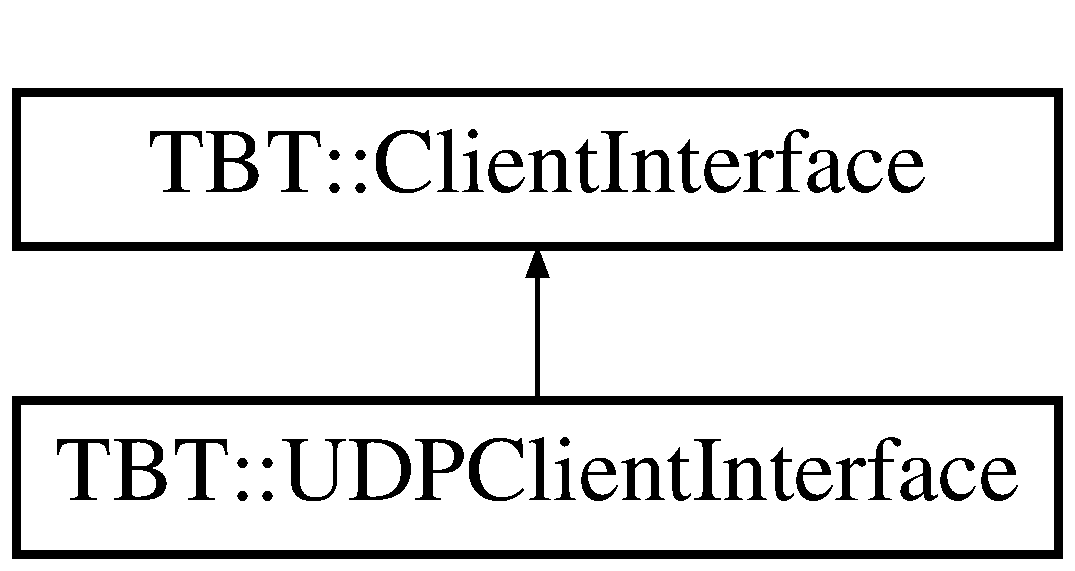
\includegraphics[height=2.000000cm]{classTBT_1_1UDPClientInterface}
\end{center}
\end{figure}
\subsection*{Public Member Functions}
\begin{DoxyCompactItemize}
\item 
\mbox{\Hypertarget{classTBT_1_1UDPClientInterface_ad03356f6abf16596c181851e9fcaf7a9}\label{classTBT_1_1UDPClientInterface_ad03356f6abf16596c181851e9fcaf7a9}} 
{\bfseries U\+D\+P\+Client\+Interface} (\hyperlink{classTBT_1_1Manager}{Manager} $\ast$p\+Manager, const in\+\_\+port\+\_\+t \&port=21105)
\item 
\mbox{\Hypertarget{classTBT_1_1UDPClientInterface_ac25b06823d045631f3c7b76e9c50f22e}\label{classTBT_1_1UDPClientInterface_ac25b06823d045631f3c7b76e9c50f22e}} 
int {\bfseries get\+My\+Socket} (void)
\item 
\mbox{\Hypertarget{classTBT_1_1UDPClientInterface_ad65d92928ce6f459c371c44c5576dbcc}\label{classTBT_1_1UDPClientInterface_ad65d92928ce6f459c371c44c5576dbcc}} 
virtual void {\bfseries broadcast\+Power\+State\+Change} (Power\+State new\+State)
\item 
\mbox{\Hypertarget{classTBT_1_1UDPClientInterface_af4e63115b3156b151d4dfd50342b36e7}\label{classTBT_1_1UDPClientInterface_af4e63115b3156b151d4dfd50342b36e7}} 
virtual void {\bfseries broadcast\+Loc\+Info\+Change} (\hyperlink{classTBT_1_1LocDecoder}{Loc\+Decoder} $\ast$p\+Loc)
\item 
\mbox{\Hypertarget{classTBT_1_1UDPClientInterface_a7fca1a79378823f67b0f23bbd59dc041}\label{classTBT_1_1UDPClientInterface_a7fca1a79378823f67b0f23bbd59dc041}} 
virtual void {\bfseries broadcast\+Emergency\+Stop} (bool state)
\end{DoxyCompactItemize}
\subsection*{Protected Member Functions}
\begin{DoxyCompactItemize}
\item 
\mbox{\Hypertarget{classTBT_1_1UDPClientInterface_aea926878d35ed4b37143e320143a84df}\label{classTBT_1_1UDPClientInterface_aea926878d35ed4b37143e320143a84df}} 
\hyperlink{classTBT_1_1UDPClient}{U\+D\+P\+Client} $\ast$ {\bfseries find\+Client} (const sockaddr\+\_\+in \&address)
\item 
\mbox{\Hypertarget{classTBT_1_1UDPClientInterface_a1a80ed1e5670443bc35691c9f3d5ff72}\label{classTBT_1_1UDPClientInterface_a1a80ed1e5670443bc35691c9f3d5ff72}} 
bool {\bfseries remove\+Client} (\hyperlink{classTBT_1_1UDPClient}{U\+D\+P\+Client} $\ast$p\+Client)
\end{DoxyCompactItemize}
\subsection*{Additional Inherited Members}


The documentation for this class was generated from the following files\+:\begin{DoxyCompactItemize}
\item 
U\+D\+P\+Client\+Interface.\+h\item 
U\+D\+P\+Client\+Interface.\+cpp\end{DoxyCompactItemize}

\hypertarget{classJson_1_1Value}{}\section{Json\+:\+:Value Class Reference}
\label{classJson_1_1Value}\index{Json\+::\+Value@{Json\+::\+Value}}


Represents a \href{http://www.json.org}{\tt J\+S\+ON} value.  




{\ttfamily \#include $<$json.\+h$>$}

\subsection*{Public Types}
\begin{DoxyCompactItemize}
\item 
\mbox{\Hypertarget{classJson_1_1Value_a9ae9069983fc38f1928d76f9c79ac64d}\label{classJson_1_1Value_a9ae9069983fc38f1928d76f9c79ac64d}} 
typedef std\+::vector$<$ J\+S\+O\+N\+C\+P\+P\+\_\+\+S\+T\+R\+I\+NG $>$ {\bfseries Members}
\item 
\mbox{\Hypertarget{classJson_1_1Value_a341cdf2e01f8b3c5b7317aa2f0768c53}\label{classJson_1_1Value_a341cdf2e01f8b3c5b7317aa2f0768c53}} 
typedef \hyperlink{classJson_1_1ValueIterator}{Value\+Iterator} {\bfseries iterator}
\item 
\mbox{\Hypertarget{classJson_1_1Value_af92282ca92b58b320debd486afb7696a}\label{classJson_1_1Value_af92282ca92b58b320debd486afb7696a}} 
typedef \hyperlink{classJson_1_1ValueConstIterator}{Value\+Const\+Iterator} {\bfseries const\+\_\+iterator}
\item 
\mbox{\Hypertarget{classJson_1_1Value_a0933d59b45793ae4aade1757c322a98d}\label{classJson_1_1Value_a0933d59b45793ae4aade1757c322a98d}} 
typedef Json\+::\+U\+Int {\bfseries U\+Int}
\item 
\mbox{\Hypertarget{classJson_1_1Value_abdf7a7ff73eb130ffcab28504ffdb405}\label{classJson_1_1Value_abdf7a7ff73eb130ffcab28504ffdb405}} 
typedef Json\+::\+Int {\bfseries Int}
\item 
\mbox{\Hypertarget{classJson_1_1Value_a8b62564be8c087c6d18de180ff4e13e3}\label{classJson_1_1Value_a8b62564be8c087c6d18de180ff4e13e3}} 
typedef Json\+::\+U\+Int64 {\bfseries U\+Int64}
\item 
\mbox{\Hypertarget{classJson_1_1Value_a1b86af9f85f0f1baa972c3319fa22695}\label{classJson_1_1Value_a1b86af9f85f0f1baa972c3319fa22695}} 
typedef Json\+::\+Int64 {\bfseries Int64}
\item 
\mbox{\Hypertarget{classJson_1_1Value_a1cbb82642ed05109b9833e49f042ece7}\label{classJson_1_1Value_a1cbb82642ed05109b9833e49f042ece7}} 
typedef Json\+::\+Largest\+Int {\bfseries Largest\+Int}
\item 
\mbox{\Hypertarget{classJson_1_1Value_a6682a3684d635e03fc06ba229fa24eec}\label{classJson_1_1Value_a6682a3684d635e03fc06ba229fa24eec}} 
typedef Json\+::\+Largest\+U\+Int {\bfseries Largest\+U\+Int}
\item 
\mbox{\Hypertarget{classJson_1_1Value_a184a91566cccca7b819240f0d5561c7d}\label{classJson_1_1Value_a184a91566cccca7b819240f0d5561c7d}} 
typedef Json\+::\+Array\+Index {\bfseries Array\+Index}
\item 
\mbox{\Hypertarget{classJson_1_1Value_a9e071ef3c135a2c9602e893b6005d0f7}\label{classJson_1_1Value_a9e071ef3c135a2c9602e893b6005d0f7}} 
typedef std\+::string {\bfseries value\+\_\+type}
\item 
\mbox{\Hypertarget{classJson_1_1Value_a08b6c80c3af7071d908dabf044de5388}\label{classJson_1_1Value_a08b6c80c3af7071d908dabf044de5388}} 
typedef std\+::map$<$ C\+Z\+String, \hyperlink{classJson_1_1Value}{Value} $>$ {\bfseries Object\+Values}
\end{DoxyCompactItemize}
\subsection*{Public Member Functions}
\begin{DoxyCompactItemize}
\item 
\hyperlink{classJson_1_1Value_ada6ba1369448fb0240bccc36efaa46f7}{Value} (\hyperlink{namespaceJson_a7d654b75c16a57007925868e38212b4e}{Value\+Type} type=\hyperlink{namespaceJson_a7d654b75c16a57007925868e38212b4ea7d9899633b4409bd3fc107e6737f8391}{null\+Value})
\begin{DoxyCompactList}\small\item\em Create a default \hyperlink{classJson_1_1Value}{Value} of the given type. \end{DoxyCompactList}\item 
\mbox{\Hypertarget{classJson_1_1Value_a4744ae571fcf34f4b16a2257b3b3b585}\label{classJson_1_1Value_a4744ae571fcf34f4b16a2257b3b3b585}} 
{\bfseries Value} (Int value)
\item 
\mbox{\Hypertarget{classJson_1_1Value_ae67a857b01286e3499a87e95be848d20}\label{classJson_1_1Value_ae67a857b01286e3499a87e95be848d20}} 
{\bfseries Value} (U\+Int value)
\item 
\mbox{\Hypertarget{classJson_1_1Value_ab1cdc3d9a4d4cc03fa01439d43ceb1b5}\label{classJson_1_1Value_ab1cdc3d9a4d4cc03fa01439d43ceb1b5}} 
{\bfseries Value} (Int64 value)
\item 
\mbox{\Hypertarget{classJson_1_1Value_a8adda58d5ae17bf7ca6a53bab4a7b69c}\label{classJson_1_1Value_a8adda58d5ae17bf7ca6a53bab4a7b69c}} 
{\bfseries Value} (U\+Int64 value)
\item 
\mbox{\Hypertarget{classJson_1_1Value_a32228cc84d83200cca8441451997996c}\label{classJson_1_1Value_a32228cc84d83200cca8441451997996c}} 
{\bfseries Value} (double value)
\item 
\mbox{\Hypertarget{classJson_1_1Value_ad87b849356816aca75995dd07302e49d}\label{classJson_1_1Value_ad87b849356816aca75995dd07302e49d}} 
\hyperlink{classJson_1_1Value_ad87b849356816aca75995dd07302e49d}{Value} (const char $\ast$value)
\begin{DoxyCompactList}\small\item\em Copy til first 0. (N\+U\+LL causes to seg-\/fault.) \end{DoxyCompactList}\item 
\mbox{\Hypertarget{classJson_1_1Value_a39fa09d1902efbd4350e1236db920571}\label{classJson_1_1Value_a39fa09d1902efbd4350e1236db920571}} 
\hyperlink{classJson_1_1Value_a39fa09d1902efbd4350e1236db920571}{Value} (const char $\ast$begin, const char $\ast$end)
\begin{DoxyCompactList}\small\item\em Copy all, incl zeroes. \end{DoxyCompactList}\item 
\hyperlink{classJson_1_1Value_a081830e95f88a37054da7e46c65b0766}{Value} (const \hyperlink{classJson_1_1StaticString}{Static\+String} \&value)
\begin{DoxyCompactList}\small\item\em Constructs a value from a static string. \end{DoxyCompactList}\item 
\mbox{\Hypertarget{classJson_1_1Value_a89ef37969ff7c6eb3a7afcca03d4cd4a}\label{classJson_1_1Value_a89ef37969ff7c6eb3a7afcca03d4cd4a}} 
\hyperlink{classJson_1_1Value_a89ef37969ff7c6eb3a7afcca03d4cd4a}{Value} (const J\+S\+O\+N\+C\+P\+P\+\_\+\+S\+T\+R\+I\+NG \&value)
\begin{DoxyCompactList}\small\item\em Copy data() til \hyperlink{classJson_1_1Value_a0ec2808e1d7efa4e9fad938d6667be44}{size()}. Embedded zeroes too. \end{DoxyCompactList}\item 
\mbox{\Hypertarget{classJson_1_1Value_a350a31ea4a30d384994b0bc010b17495}\label{classJson_1_1Value_a350a31ea4a30d384994b0bc010b17495}} 
{\bfseries Value} (bool value)
\item 
\mbox{\Hypertarget{classJson_1_1Value_a436dfd3670f95fd665f680eba5cebcf0}\label{classJson_1_1Value_a436dfd3670f95fd665f680eba5cebcf0}} 
\hyperlink{classJson_1_1Value_a436dfd3670f95fd665f680eba5cebcf0}{Value} (const \hyperlink{classJson_1_1Value}{Value} \&other)
\begin{DoxyCompactList}\small\item\em Deep copy. \end{DoxyCompactList}\item 
\hyperlink{classJson_1_1Value}{Value} \& \hyperlink{classJson_1_1Value_a795acb28772da4c5d85ae8f4af36c69f}{operator=} (\hyperlink{classJson_1_1Value}{Value} other)
\item 
\mbox{\Hypertarget{classJson_1_1Value_aab841120d78e296e1bc06a373345e822}\label{classJson_1_1Value_aab841120d78e296e1bc06a373345e822}} 
void \hyperlink{classJson_1_1Value_aab841120d78e296e1bc06a373345e822}{swap} (\hyperlink{classJson_1_1Value}{Value} \&other)
\begin{DoxyCompactList}\small\item\em Swap everything. \end{DoxyCompactList}\item 
\mbox{\Hypertarget{classJson_1_1Value_a5263476047f20e2fc6de470e4de34fe5}\label{classJson_1_1Value_a5263476047f20e2fc6de470e4de34fe5}} 
void \hyperlink{classJson_1_1Value_a5263476047f20e2fc6de470e4de34fe5}{swap\+Payload} (\hyperlink{classJson_1_1Value}{Value} \&other)
\begin{DoxyCompactList}\small\item\em Swap values but leave comments and source offsets in place. \end{DoxyCompactList}\item 
\mbox{\Hypertarget{classJson_1_1Value_a1b2c6379664d91b9f1bcd4d1853e5970}\label{classJson_1_1Value_a1b2c6379664d91b9f1bcd4d1853e5970}} 
void \hyperlink{classJson_1_1Value_a1b2c6379664d91b9f1bcd4d1853e5970}{copy} (const \hyperlink{classJson_1_1Value}{Value} \&other)
\begin{DoxyCompactList}\small\item\em copy everything. \end{DoxyCompactList}\item 
\mbox{\Hypertarget{classJson_1_1Value_ab504d299cfaa440392037fa8a3c54064}\label{classJson_1_1Value_ab504d299cfaa440392037fa8a3c54064}} 
void \hyperlink{classJson_1_1Value_ab504d299cfaa440392037fa8a3c54064}{copy\+Payload} (const \hyperlink{classJson_1_1Value}{Value} \&other)
\begin{DoxyCompactList}\small\item\em copy values but leave comments and source offsets in place. \end{DoxyCompactList}\item 
\mbox{\Hypertarget{classJson_1_1Value_a8ce61157a011894f0252ceed232312de}\label{classJson_1_1Value_a8ce61157a011894f0252ceed232312de}} 
\hyperlink{namespaceJson_a7d654b75c16a57007925868e38212b4e}{Value\+Type} {\bfseries type} () const
\item 
\mbox{\Hypertarget{classJson_1_1Value_aac6bd14155b88ed2d39ef54820b39e49}\label{classJson_1_1Value_aac6bd14155b88ed2d39ef54820b39e49}} 
bool \hyperlink{classJson_1_1Value_aac6bd14155b88ed2d39ef54820b39e49}{operator$<$} (const \hyperlink{classJson_1_1Value}{Value} \&other) const
\begin{DoxyCompactList}\small\item\em Compare payload only, not comments etc. \end{DoxyCompactList}\item 
\mbox{\Hypertarget{classJson_1_1Value_a40c411a320a416d5eac0052b36211286}\label{classJson_1_1Value_a40c411a320a416d5eac0052b36211286}} 
bool {\bfseries operator$<$=} (const \hyperlink{classJson_1_1Value}{Value} \&other) const
\item 
\mbox{\Hypertarget{classJson_1_1Value_afe2c3e52df60b9622cbd8358b74bdbf5}\label{classJson_1_1Value_afe2c3e52df60b9622cbd8358b74bdbf5}} 
bool {\bfseries operator$>$=} (const \hyperlink{classJson_1_1Value}{Value} \&other) const
\item 
\mbox{\Hypertarget{classJson_1_1Value_a4646c2f0764908c0972160c7c2ebe567}\label{classJson_1_1Value_a4646c2f0764908c0972160c7c2ebe567}} 
bool {\bfseries operator$>$} (const \hyperlink{classJson_1_1Value}{Value} \&other) const
\item 
\mbox{\Hypertarget{classJson_1_1Value_a16f9250e30d5c4505cd11137c564a764}\label{classJson_1_1Value_a16f9250e30d5c4505cd11137c564a764}} 
bool {\bfseries operator==} (const \hyperlink{classJson_1_1Value}{Value} \&other) const
\item 
\mbox{\Hypertarget{classJson_1_1Value_a86e95be072e515c48abc61dec63a1689}\label{classJson_1_1Value_a86e95be072e515c48abc61dec63a1689}} 
bool {\bfseries operator!=} (const \hyperlink{classJson_1_1Value}{Value} \&other) const
\item 
\mbox{\Hypertarget{classJson_1_1Value_aefa4464ca1bb0bcc9a87b38ed62ca2e0}\label{classJson_1_1Value_aefa4464ca1bb0bcc9a87b38ed62ca2e0}} 
int {\bfseries compare} (const \hyperlink{classJson_1_1Value}{Value} \&other) const
\item 
\mbox{\Hypertarget{classJson_1_1Value_a16668c8db7ef0a5de040012f0dfd84b0}\label{classJson_1_1Value_a16668c8db7ef0a5de040012f0dfd84b0}} 
const char $\ast$ \hyperlink{classJson_1_1Value_a16668c8db7ef0a5de040012f0dfd84b0}{as\+C\+String} () const
\begin{DoxyCompactList}\small\item\em Embedded zeroes could cause you trouble! \end{DoxyCompactList}\item 
\mbox{\Hypertarget{classJson_1_1Value_ae3f9b0d38f820ccdd8888aa92ea6e792}\label{classJson_1_1Value_ae3f9b0d38f820ccdd8888aa92ea6e792}} 
J\+S\+O\+N\+C\+P\+P\+\_\+\+S\+T\+R\+I\+NG \hyperlink{classJson_1_1Value_ae3f9b0d38f820ccdd8888aa92ea6e792}{as\+String} () const
\begin{DoxyCompactList}\small\item\em Embedded zeroes are possible. \end{DoxyCompactList}\item 
bool \hyperlink{classJson_1_1Value_a2e1b7be6bde2fe23f15290d9ddbbdf8a}{get\+String} (char const $\ast$$\ast$begin, char const $\ast$$\ast$end) const
\item 
\mbox{\Hypertarget{classJson_1_1Value_a614d635bc248a592593feb322cd15ab8}\label{classJson_1_1Value_a614d635bc248a592593feb322cd15ab8}} 
Int {\bfseries as\+Int} () const
\item 
\mbox{\Hypertarget{classJson_1_1Value_a74b305583ec3aacf4f9dd06e799dc265}\label{classJson_1_1Value_a74b305583ec3aacf4f9dd06e799dc265}} 
U\+Int {\bfseries as\+U\+Int} () const
\item 
\mbox{\Hypertarget{classJson_1_1Value_aa647ac4fe51a2e325c063ebe32262b44}\label{classJson_1_1Value_aa647ac4fe51a2e325c063ebe32262b44}} 
Int64 {\bfseries as\+Int64} () const
\item 
\mbox{\Hypertarget{classJson_1_1Value_a0e44a5a4cd0c099f9570dfa25813eb60}\label{classJson_1_1Value_a0e44a5a4cd0c099f9570dfa25813eb60}} 
U\+Int64 {\bfseries as\+U\+Int64} () const
\item 
\mbox{\Hypertarget{classJson_1_1Value_ab16f2ea2a117a1b3b576acab8b6a700d}\label{classJson_1_1Value_ab16f2ea2a117a1b3b576acab8b6a700d}} 
Largest\+Int {\bfseries as\+Largest\+Int} () const
\item 
\mbox{\Hypertarget{classJson_1_1Value_ad03548101e0bf3d2d9eac75c64a0b8d7}\label{classJson_1_1Value_ad03548101e0bf3d2d9eac75c64a0b8d7}} 
Largest\+U\+Int {\bfseries as\+Largest\+U\+Int} () const
\item 
\mbox{\Hypertarget{classJson_1_1Value_af3a4d10bf575fabdc5440a7135c9649c}\label{classJson_1_1Value_af3a4d10bf575fabdc5440a7135c9649c}} 
float {\bfseries as\+Float} () const
\item 
\mbox{\Hypertarget{classJson_1_1Value_afd24002a18aef907ad746b1cb9eda0a2}\label{classJson_1_1Value_afd24002a18aef907ad746b1cb9eda0a2}} 
double {\bfseries as\+Double} () const
\item 
\mbox{\Hypertarget{classJson_1_1Value_ab693fb7b9b1595bb0adc49658bbf780d}\label{classJson_1_1Value_ab693fb7b9b1595bb0adc49658bbf780d}} 
bool {\bfseries as\+Bool} () const
\item 
\mbox{\Hypertarget{classJson_1_1Value_abde4070e21e46dc4f8203f66582cb19f}\label{classJson_1_1Value_abde4070e21e46dc4f8203f66582cb19f}} 
bool {\bfseries is\+Null} () const
\item 
\mbox{\Hypertarget{classJson_1_1Value_ab1f02651cb89d0f18b63a036959391ba}\label{classJson_1_1Value_ab1f02651cb89d0f18b63a036959391ba}} 
bool {\bfseries is\+Bool} () const
\item 
\mbox{\Hypertarget{classJson_1_1Value_aff51d8b52979ca06cf9d909accd5f695}\label{classJson_1_1Value_aff51d8b52979ca06cf9d909accd5f695}} 
bool {\bfseries is\+Int} () const
\item 
\mbox{\Hypertarget{classJson_1_1Value_a4a81fb3c3acdbb68b2e2f30836a4f53e}\label{classJson_1_1Value_a4a81fb3c3acdbb68b2e2f30836a4f53e}} 
bool {\bfseries is\+Int64} () const
\item 
\mbox{\Hypertarget{classJson_1_1Value_abdda463d3269015f883587349726cfbc}\label{classJson_1_1Value_abdda463d3269015f883587349726cfbc}} 
bool {\bfseries is\+U\+Int} () const
\item 
\mbox{\Hypertarget{classJson_1_1Value_a883576e35cb03a785258edb56777a2de}\label{classJson_1_1Value_a883576e35cb03a785258edb56777a2de}} 
bool {\bfseries is\+U\+Int64} () const
\item 
\mbox{\Hypertarget{classJson_1_1Value_ab6798954f6e80281cf22708ef45198a7}\label{classJson_1_1Value_ab6798954f6e80281cf22708ef45198a7}} 
bool {\bfseries is\+Integral} () const
\item 
\mbox{\Hypertarget{classJson_1_1Value_a4a2e2a790e19a1c09fc5dd12d7ad47b5}\label{classJson_1_1Value_a4a2e2a790e19a1c09fc5dd12d7ad47b5}} 
bool {\bfseries is\+Double} () const
\item 
\mbox{\Hypertarget{classJson_1_1Value_af961a000cd203c895e44c195ab39b866}\label{classJson_1_1Value_af961a000cd203c895e44c195ab39b866}} 
bool {\bfseries is\+Numeric} () const
\item 
\mbox{\Hypertarget{classJson_1_1Value_a71e1f82cf1c3eaf969d400dcffb163a6}\label{classJson_1_1Value_a71e1f82cf1c3eaf969d400dcffb163a6}} 
bool {\bfseries is\+String} () const
\item 
\mbox{\Hypertarget{classJson_1_1Value_a1627eb9d6568d6d0252fa8bb711c0a59}\label{classJson_1_1Value_a1627eb9d6568d6d0252fa8bb711c0a59}} 
bool {\bfseries is\+Array} () const
\item 
\mbox{\Hypertarget{classJson_1_1Value_a8cf96c0f2a552051fcfc78ffee60e037}\label{classJson_1_1Value_a8cf96c0f2a552051fcfc78ffee60e037}} 
bool {\bfseries is\+Object} () const
\item 
\mbox{\Hypertarget{classJson_1_1Value_af1ee6be27a96a7d12128efdd60deb54d}\label{classJson_1_1Value_af1ee6be27a96a7d12128efdd60deb54d}} 
bool {\bfseries is\+Convertible\+To} (\hyperlink{namespaceJson_a7d654b75c16a57007925868e38212b4e}{Value\+Type} other) const
\item 
\mbox{\Hypertarget{classJson_1_1Value_a0ec2808e1d7efa4e9fad938d6667be44}\label{classJson_1_1Value_a0ec2808e1d7efa4e9fad938d6667be44}} 
Array\+Index \hyperlink{classJson_1_1Value_a0ec2808e1d7efa4e9fad938d6667be44}{size} () const
\begin{DoxyCompactList}\small\item\em Number of values in array or object. \end{DoxyCompactList}\item 
\mbox{\Hypertarget{classJson_1_1Value_a0519a551e37ee6665d74742b3f96bab3}\label{classJson_1_1Value_a0519a551e37ee6665d74742b3f96bab3}} 
bool \hyperlink{classJson_1_1Value_a0519a551e37ee6665d74742b3f96bab3}{empty} () const
\begin{DoxyCompactList}\small\item\em Return true if empty array, empty object, or null; otherwise, false. \end{DoxyCompactList}\item 
\mbox{\Hypertarget{classJson_1_1Value_a731b89fb4764c39ce2328e1707c822b9}\label{classJson_1_1Value_a731b89fb4764c39ce2328e1707c822b9}} 
bool \hyperlink{classJson_1_1Value_a731b89fb4764c39ce2328e1707c822b9}{operator!} () const
\begin{DoxyCompactList}\small\item\em Return is\+Null() \end{DoxyCompactList}\item 
void \hyperlink{classJson_1_1Value_a501a4d67e6c875255c2ecc03ccd2019b}{clear} ()
\item 
void \hyperlink{classJson_1_1Value_aa284353271ada427dbfa04a42f2be407}{resize} (Array\+Index \hyperlink{classJson_1_1Value_a0ec2808e1d7efa4e9fad938d6667be44}{size})
\item 
\hyperlink{classJson_1_1Value}{Value} \& \hyperlink{classJson_1_1Value_a7d99f5dba388cdaa152ce6ef933d64ef}{operator\mbox{[}$\,$\mbox{]}} (Array\+Index index)
\item 
\hyperlink{classJson_1_1Value}{Value} \& \hyperlink{classJson_1_1Value_ac9182982c361e0ab621134d406e5f250}{operator\mbox{[}$\,$\mbox{]}} (int index)
\item 
const \hyperlink{classJson_1_1Value}{Value} \& \hyperlink{classJson_1_1Value_a46607236038b29695ed80c15895271e4}{operator\mbox{[}$\,$\mbox{]}} (Array\+Index index) const
\item 
const \hyperlink{classJson_1_1Value}{Value} \& \hyperlink{classJson_1_1Value_a0b42557a95621a4676b46a21ffc5e949}{operator\mbox{[}$\,$\mbox{]}} (int index) const
\item 
\hyperlink{classJson_1_1Value}{Value} \hyperlink{classJson_1_1Value_a034eb7bf85a44fa759bdaa232788ca66}{get} (Array\+Index index, const \hyperlink{classJson_1_1Value}{Value} \&default\+Value) const
\item 
\mbox{\Hypertarget{classJson_1_1Value_ac2928f174a6e081c1500c28c2d61ee93}\label{classJson_1_1Value_ac2928f174a6e081c1500c28c2d61ee93}} 
bool \hyperlink{classJson_1_1Value_ac2928f174a6e081c1500c28c2d61ee93}{is\+Valid\+Index} (Array\+Index index) const
\begin{DoxyCompactList}\small\item\em Return true if index $<$ \hyperlink{classJson_1_1Value_a0ec2808e1d7efa4e9fad938d6667be44}{size()}. \end{DoxyCompactList}\item 
\hyperlink{classJson_1_1Value}{Value} \& \hyperlink{classJson_1_1Value_a7e49ac977e4bcf59745a09d426669f75}{append} (const \hyperlink{classJson_1_1Value}{Value} \&value)
\begin{DoxyCompactList}\small\item\em Append value to array at the end. \end{DoxyCompactList}\item 
\hyperlink{classJson_1_1Value}{Value} \& \hyperlink{classJson_1_1Value_acb912f4ec40a25ea6eb387730885f3d9}{operator\mbox{[}$\,$\mbox{]}} (const char $\ast$key)
\item 
const \hyperlink{classJson_1_1Value}{Value} \& \hyperlink{classJson_1_1Value_a1b0498b7b2a520a68137f682d91abdd5}{operator\mbox{[}$\,$\mbox{]}} (const char $\ast$key) const
\item 
\hyperlink{classJson_1_1Value}{Value} \& \hyperlink{classJson_1_1Value_aedd1e152756a4cc8c1ebac0dd7aeeb78}{operator\mbox{[}$\,$\mbox{]}} (const J\+S\+O\+N\+C\+P\+P\+\_\+\+S\+T\+R\+I\+NG \&key)
\item 
const \hyperlink{classJson_1_1Value}{Value} \& \hyperlink{classJson_1_1Value_aba60f69dcd85e935aa85e7a517e03427}{operator\mbox{[}$\,$\mbox{]}} (const J\+S\+O\+N\+C\+P\+P\+\_\+\+S\+T\+R\+I\+NG \&key) const
\item 
\hyperlink{classJson_1_1Value}{Value} \& \hyperlink{classJson_1_1Value_ac3763d7d315ca65dc188e273722f7955}{operator\mbox{[}$\,$\mbox{]}} (const \hyperlink{classJson_1_1StaticString}{Static\+String} \&key)
\begin{DoxyCompactList}\small\item\em Access an object value by name, create a null member if it does not exist. \end{DoxyCompactList}\item 
\hyperlink{classJson_1_1Value}{Value} \hyperlink{classJson_1_1Value_a57de86629ed23246f14014fb6c44fa67}{get} (const char $\ast$key, const \hyperlink{classJson_1_1Value}{Value} \&default\+Value) const
\item 
\hyperlink{classJson_1_1Value}{Value} \hyperlink{classJson_1_1Value_aa59ed050e87e1d58d93671a38687f36c}{get} (const char $\ast$begin, const char $\ast$end, const \hyperlink{classJson_1_1Value}{Value} \&default\+Value) const
\item 
\hyperlink{classJson_1_1Value}{Value} \hyperlink{classJson_1_1Value_a7406e6af727c288bf8ab59945ece686a}{get} (const J\+S\+O\+N\+C\+P\+P\+\_\+\+S\+T\+R\+I\+NG \&key, const \hyperlink{classJson_1_1Value}{Value} \&default\+Value) const
\item 
\hyperlink{classJson_1_1Value}{Value} const  $\ast$ \hyperlink{classJson_1_1Value_afb007b9ce9b2cf9d5f667a07e5e0349f}{find} (char const $\ast$begin, char const $\ast$end) const
\item 
\hyperlink{classJson_1_1Value}{Value} const  $\ast$ \hyperlink{classJson_1_1Value_afeb7ff596a0929d90c5f2f3cffb413ed}{demand} (char const $\ast$begin, char const $\ast$end)
\item 
void \hyperlink{classJson_1_1Value_a92e165f04105d27a930fb3a18a053585}{remove\+Member} (const char $\ast$key)
\begin{DoxyCompactList}\small\item\em Remove and return the named member. \end{DoxyCompactList}\item 
void \hyperlink{classJson_1_1Value_a8a660202bbad35857b39e85bd35ec78a}{remove\+Member} (const J\+S\+O\+N\+C\+P\+P\+\_\+\+S\+T\+R\+I\+NG \&key)
\item 
bool \hyperlink{classJson_1_1Value_a708e599489adf30d65bf85a8ee16e6fb}{remove\+Member} (const char $\ast$key, \hyperlink{classJson_1_1Value}{Value} $\ast$removed)
\item 
bool \hyperlink{classJson_1_1Value_ae385ecef98427970df525ee876e9f54a}{remove\+Member} (J\+S\+O\+N\+C\+P\+P\+\_\+\+S\+T\+R\+I\+NG const \&key, \hyperlink{classJson_1_1Value}{Value} $\ast$removed)
\begin{DoxyCompactList}\small\item\em Remove the named map member. \end{DoxyCompactList}\item 
\mbox{\Hypertarget{classJson_1_1Value_a49c91af727d6b4eb0af02a81bb2def87}\label{classJson_1_1Value_a49c91af727d6b4eb0af02a81bb2def87}} 
bool \hyperlink{classJson_1_1Value_a49c91af727d6b4eb0af02a81bb2def87}{remove\+Member} (const char $\ast$begin, const char $\ast$end, \hyperlink{classJson_1_1Value}{Value} $\ast$removed)
\begin{DoxyCompactList}\small\item\em Same as \hyperlink{classJson_1_1Value_ae385ecef98427970df525ee876e9f54a}{remove\+Member(\+J\+S\+O\+N\+C\+P\+P\+\_\+\+S\+T\+R\+I\+N\+G const\& key, Value$\ast$ removed)} \end{DoxyCompactList}\item 
bool \hyperlink{classJson_1_1Value_ae9e67e08a85a2f3be3396ec0f4c47f65}{remove\+Index} (Array\+Index i, \hyperlink{classJson_1_1Value}{Value} $\ast$removed)
\begin{DoxyCompactList}\small\item\em Remove the indexed array element. \end{DoxyCompactList}\item 
bool \hyperlink{classJson_1_1Value_ad6d4df2227321bab05e86667609a7fad}{is\+Member} (const char $\ast$key) const
\item 
bool \hyperlink{classJson_1_1Value_a0c2cd838217b23ee6bde8135de1b30d9}{is\+Member} (const J\+S\+O\+N\+C\+P\+P\+\_\+\+S\+T\+R\+I\+NG \&key) const
\item 
\mbox{\Hypertarget{classJson_1_1Value_a2007e1e51f21f44ecf1f13e4a1c567b9}\label{classJson_1_1Value_a2007e1e51f21f44ecf1f13e4a1c567b9}} 
bool \hyperlink{classJson_1_1Value_a2007e1e51f21f44ecf1f13e4a1c567b9}{is\+Member} (const char $\ast$begin, const char $\ast$end) const
\begin{DoxyCompactList}\small\item\em Same as \hyperlink{classJson_1_1Value_a0c2cd838217b23ee6bde8135de1b30d9}{is\+Member(\+J\+S\+O\+N\+C\+P\+P\+\_\+\+S\+T\+R\+I\+N\+G const\& key)const}. \end{DoxyCompactList}\item 
Members \hyperlink{classJson_1_1Value_a79d7725dce6260317333e69022367ac9}{get\+Member\+Names} () const
\begin{DoxyCompactList}\small\item\em Return a list of the member names. \end{DoxyCompactList}\item 
void \hyperlink{classJson_1_1Value_a29f3a30f7e5d3af6f38d57999bf5b480}{set\+Comment} (const char $\ast$comment, \hyperlink{namespaceJson_a4fc417c23905b2ae9e2c47d197a45351}{Comment\+Placement} placement)
\item 
\mbox{\Hypertarget{classJson_1_1Value_a2900152a2887b410a9ddabe278b9d492}\label{classJson_1_1Value_a2900152a2887b410a9ddabe278b9d492}} 
void \hyperlink{classJson_1_1Value_a2900152a2887b410a9ddabe278b9d492}{set\+Comment} (const char $\ast$comment, size\+\_\+t len, \hyperlink{namespaceJson_a4fc417c23905b2ae9e2c47d197a45351}{Comment\+Placement} placement)
\begin{DoxyCompactList}\small\item\em Comments must be //... or /$\ast$ ... $\ast$/. \end{DoxyCompactList}\item 
\mbox{\Hypertarget{classJson_1_1Value_a2c5d13a5f45eb77e912008778e65b27f}\label{classJson_1_1Value_a2c5d13a5f45eb77e912008778e65b27f}} 
void \hyperlink{classJson_1_1Value_a2c5d13a5f45eb77e912008778e65b27f}{set\+Comment} (const J\+S\+O\+N\+C\+P\+P\+\_\+\+S\+T\+R\+I\+NG \&comment, \hyperlink{namespaceJson_a4fc417c23905b2ae9e2c47d197a45351}{Comment\+Placement} placement)
\begin{DoxyCompactList}\small\item\em Comments must be //... or /$\ast$ ... $\ast$/. \end{DoxyCompactList}\item 
\mbox{\Hypertarget{classJson_1_1Value_a65d8e3ab6a5871cbd019a3e0f0b944a3}\label{classJson_1_1Value_a65d8e3ab6a5871cbd019a3e0f0b944a3}} 
bool {\bfseries has\+Comment} (\hyperlink{namespaceJson_a4fc417c23905b2ae9e2c47d197a45351}{Comment\+Placement} placement) const
\item 
\mbox{\Hypertarget{classJson_1_1Value_a82817229a986f0b254e31d5c83066ffe}\label{classJson_1_1Value_a82817229a986f0b254e31d5c83066ffe}} 
J\+S\+O\+N\+C\+P\+P\+\_\+\+S\+T\+R\+I\+NG \hyperlink{classJson_1_1Value_a82817229a986f0b254e31d5c83066ffe}{get\+Comment} (\hyperlink{namespaceJson_a4fc417c23905b2ae9e2c47d197a45351}{Comment\+Placement} placement) const
\begin{DoxyCompactList}\small\item\em Include delimiters and embedded newlines. \end{DoxyCompactList}\item 
\mbox{\Hypertarget{classJson_1_1Value_a00154cc8662d7a845ed59e175c2496cb}\label{classJson_1_1Value_a00154cc8662d7a845ed59e175c2496cb}} 
J\+S\+O\+N\+C\+P\+P\+\_\+\+S\+T\+R\+I\+NG {\bfseries to\+Styled\+String} () const
\item 
\mbox{\Hypertarget{classJson_1_1Value_a015459a3950c198d63a2d3be8f5ae296}\label{classJson_1_1Value_a015459a3950c198d63a2d3be8f5ae296}} 
\hyperlink{classJson_1_1ValueConstIterator}{const\+\_\+iterator} {\bfseries begin} () const
\item 
\mbox{\Hypertarget{classJson_1_1Value_a3e443cd0ef24f7e028b175e47ee045e0}\label{classJson_1_1Value_a3e443cd0ef24f7e028b175e47ee045e0}} 
\hyperlink{classJson_1_1ValueConstIterator}{const\+\_\+iterator} {\bfseries end} () const
\item 
\mbox{\Hypertarget{classJson_1_1Value_a2d45bb2e68e8f22fe356d7d955ebd3c9}\label{classJson_1_1Value_a2d45bb2e68e8f22fe356d7d955ebd3c9}} 
\hyperlink{classJson_1_1ValueIterator}{iterator} {\bfseries begin} ()
\item 
\mbox{\Hypertarget{classJson_1_1Value_a2f961eff73f7f79cd29260b6cbd42558}\label{classJson_1_1Value_a2f961eff73f7f79cd29260b6cbd42558}} 
\hyperlink{classJson_1_1ValueIterator}{iterator} {\bfseries end} ()
\item 
\mbox{\Hypertarget{classJson_1_1Value_a92e32ea0f4f8a15853a3cf0beac9feb9}\label{classJson_1_1Value_a92e32ea0f4f8a15853a3cf0beac9feb9}} 
void {\bfseries set\+Offset\+Start} (ptrdiff\+\_\+t start)
\item 
\mbox{\Hypertarget{classJson_1_1Value_a5e4f5853fec138150c5df6004a8c2bcf}\label{classJson_1_1Value_a5e4f5853fec138150c5df6004a8c2bcf}} 
void {\bfseries set\+Offset\+Limit} (ptrdiff\+\_\+t limit)
\item 
\mbox{\Hypertarget{classJson_1_1Value_afa081dc764000951a1d8d6148155508e}\label{classJson_1_1Value_afa081dc764000951a1d8d6148155508e}} 
ptrdiff\+\_\+t {\bfseries get\+Offset\+Start} () const
\item 
\mbox{\Hypertarget{classJson_1_1Value_a2cdfa01935f87fcace90d450cbd2c0a4}\label{classJson_1_1Value_a2cdfa01935f87fcace90d450cbd2c0a4}} 
ptrdiff\+\_\+t {\bfseries get\+Offset\+Limit} () const
\end{DoxyCompactItemize}
\subsection*{Static Public Member Functions}
\begin{DoxyCompactItemize}
\item 
\mbox{\Hypertarget{classJson_1_1Value_af2f124567acc35d021a424e53ebdfcab}\label{classJson_1_1Value_af2f124567acc35d021a424e53ebdfcab}} 
static \hyperlink{classJson_1_1Value}{Value} const  \& \hyperlink{classJson_1_1Value_af2f124567acc35d021a424e53ebdfcab}{null\+Singleton} ()
\begin{DoxyCompactList}\small\item\em Prefer this to null or null\+Ref. \end{DoxyCompactList}\end{DoxyCompactItemize}
\subsection*{Static Public Attributes}
\begin{DoxyCompactItemize}
\item 
\mbox{\Hypertarget{classJson_1_1Value_a21ddb05b92c60c7548e928bf371e7d45}\label{classJson_1_1Value_a21ddb05b92c60c7548e928bf371e7d45}} 
static const \hyperlink{classJson_1_1Value}{Value} \& \hyperlink{classJson_1_1Value_a21ddb05b92c60c7548e928bf371e7d45}{null} = \hyperlink{classJson_1_1Value_af2f124567acc35d021a424e53ebdfcab}{Value\+::null\+Singleton}()
\begin{DoxyCompactList}\small\item\em We regret this reference to a global instance; prefer the simpler \hyperlink{classJson_1_1Value_ada6ba1369448fb0240bccc36efaa46f7}{Value()}. \end{DoxyCompactList}\item 
\mbox{\Hypertarget{classJson_1_1Value_aaee27e622f87266f861216d644603730}\label{classJson_1_1Value_aaee27e622f87266f861216d644603730}} 
static const \hyperlink{classJson_1_1Value}{Value} \& \hyperlink{classJson_1_1Value_aaee27e622f87266f861216d644603730}{null\+Ref} = \hyperlink{classJson_1_1Value_af2f124567acc35d021a424e53ebdfcab}{Value\+::null\+Singleton}()
\begin{DoxyCompactList}\small\item\em just a kludge for binary-\/compatibility; same as null \end{DoxyCompactList}\item 
\mbox{\Hypertarget{classJson_1_1Value_af91df130daa50dd43d2cd89e6ee67706}\label{classJson_1_1Value_af91df130daa50dd43d2cd89e6ee67706}} 
static const Largest\+Int \hyperlink{classJson_1_1Value_af91df130daa50dd43d2cd89e6ee67706}{min\+Largest\+Int} = Largest\+Int($\sim$(Largest\+U\+Int(-\/1) / 2))
\begin{DoxyCompactList}\small\item\em Minimum signed integer value that can be stored in a \hyperlink{classJson_1_1Value}{Json\+::\+Value}. \end{DoxyCompactList}\item 
\mbox{\Hypertarget{classJson_1_1Value_a8b4977696f13296fa8755c7953fafb2f}\label{classJson_1_1Value_a8b4977696f13296fa8755c7953fafb2f}} 
static const Largest\+Int \hyperlink{classJson_1_1Value_a8b4977696f13296fa8755c7953fafb2f}{max\+Largest\+Int} = Largest\+Int(Largest\+U\+Int(-\/1) / 2)
\begin{DoxyCompactList}\small\item\em Maximum signed integer value that can be stored in a \hyperlink{classJson_1_1Value}{Json\+::\+Value}. \end{DoxyCompactList}\item 
\mbox{\Hypertarget{classJson_1_1Value_a8ddb32d9d55fa5323ae5135639dc2e31}\label{classJson_1_1Value_a8ddb32d9d55fa5323ae5135639dc2e31}} 
static const Largest\+U\+Int \hyperlink{classJson_1_1Value_a8ddb32d9d55fa5323ae5135639dc2e31}{max\+Largest\+U\+Int} = Largest\+U\+Int(-\/1)
\begin{DoxyCompactList}\small\item\em Maximum unsigned integer value that can be stored in a \hyperlink{classJson_1_1Value}{Json\+::\+Value}. \end{DoxyCompactList}\item 
\mbox{\Hypertarget{classJson_1_1Value_a7df8a39e2502b8c92a6a41e3d752d2c8}\label{classJson_1_1Value_a7df8a39e2502b8c92a6a41e3d752d2c8}} 
static const Int \hyperlink{classJson_1_1Value_a7df8a39e2502b8c92a6a41e3d752d2c8}{min\+Int} = Int($\sim$(U\+Int(-\/1) / 2))
\begin{DoxyCompactList}\small\item\em Minimum signed int value that can be stored in a \hyperlink{classJson_1_1Value}{Json\+::\+Value}. \end{DoxyCompactList}\item 
\mbox{\Hypertarget{classJson_1_1Value_a978c799a8af3114ef7dab6fd0a310a1b}\label{classJson_1_1Value_a978c799a8af3114ef7dab6fd0a310a1b}} 
static const Int \hyperlink{classJson_1_1Value_a978c799a8af3114ef7dab6fd0a310a1b}{max\+Int} = Int(U\+Int(-\/1) / 2)
\begin{DoxyCompactList}\small\item\em Maximum signed int value that can be stored in a \hyperlink{classJson_1_1Value}{Json\+::\+Value}. \end{DoxyCompactList}\item 
\mbox{\Hypertarget{classJson_1_1Value_ac79e63ee68d3aa914bfd6988be669b87}\label{classJson_1_1Value_ac79e63ee68d3aa914bfd6988be669b87}} 
static const U\+Int \hyperlink{classJson_1_1Value_ac79e63ee68d3aa914bfd6988be669b87}{max\+U\+Int} = U\+Int(-\/1)
\begin{DoxyCompactList}\small\item\em Maximum unsigned int value that can be stored in a \hyperlink{classJson_1_1Value}{Json\+::\+Value}. \end{DoxyCompactList}\item 
\mbox{\Hypertarget{classJson_1_1Value_a815ef899bc312c93bc426511acfe31a7}\label{classJson_1_1Value_a815ef899bc312c93bc426511acfe31a7}} 
static const Int64 \hyperlink{classJson_1_1Value_a815ef899bc312c93bc426511acfe31a7}{min\+Int64} = Int64($\sim$(U\+Int64(-\/1) / 2))
\begin{DoxyCompactList}\small\item\em Minimum signed 64 bits int value that can be stored in a \hyperlink{classJson_1_1Value}{Json\+::\+Value}. \end{DoxyCompactList}\item 
\mbox{\Hypertarget{classJson_1_1Value_a4492634870b8c5709ce967b384ac6006}\label{classJson_1_1Value_a4492634870b8c5709ce967b384ac6006}} 
static const Int64 \hyperlink{classJson_1_1Value_a4492634870b8c5709ce967b384ac6006}{max\+Int64} = Int64(U\+Int64(-\/1) / 2)
\begin{DoxyCompactList}\small\item\em Maximum signed 64 bits int value that can be stored in a \hyperlink{classJson_1_1Value}{Json\+::\+Value}. \end{DoxyCompactList}\item 
\mbox{\Hypertarget{classJson_1_1Value_ae1eb89c305c39516696ff305cffa01da}\label{classJson_1_1Value_ae1eb89c305c39516696ff305cffa01da}} 
static const U\+Int64 \hyperlink{classJson_1_1Value_ae1eb89c305c39516696ff305cffa01da}{max\+U\+Int64} = U\+Int64(-\/1)
\begin{DoxyCompactList}\small\item\em Maximum unsigned 64 bits int value that can be stored in a \hyperlink{classJson_1_1Value}{Json\+::\+Value}. \end{DoxyCompactList}\end{DoxyCompactItemize}
\subsection*{Friends}
\begin{DoxyCompactItemize}
\item 
\mbox{\Hypertarget{classJson_1_1Value_ad016df56489e5d360735457afba2f649}\label{classJson_1_1Value_ad016df56489e5d360735457afba2f649}} 
class {\bfseries Value\+Iterator\+Base}
\end{DoxyCompactItemize}


\subsection{Detailed Description}
Represents a \href{http://www.json.org}{\tt J\+S\+ON} value. 

This class is a discriminated union wrapper that can represents a\+:
\begin{DoxyItemize}
\item signed integer \mbox{[}range\+: \hyperlink{classJson_1_1Value_a7df8a39e2502b8c92a6a41e3d752d2c8}{Value\+::min\+Int} -\/ \hyperlink{classJson_1_1Value_a978c799a8af3114ef7dab6fd0a310a1b}{Value\+::max\+Int}\mbox{]}
\item unsigned integer (range\+: 0 -\/ \hyperlink{classJson_1_1Value_ac79e63ee68d3aa914bfd6988be669b87}{Value\+::max\+U\+Int})
\item double
\item U\+T\+F-\/8 string
\item boolean
\item \textquotesingle{}null\textquotesingle{}
\item an ordered list of \hyperlink{classJson_1_1Value}{Value}
\item collection of name/value pairs (javascript object)
\end{DoxyItemize}

The type of the held value is represented by a \hyperlink{namespaceJson_a7d654b75c16a57007925868e38212b4e}{Value\+Type} and can be obtained using type().

Values of an \hyperlink{namespaceJson_a7d654b75c16a57007925868e38212b4eae8386dcfc36d1ae897745f7b4f77a1f6}{object\+Value} or \hyperlink{namespaceJson_a7d654b75c16a57007925868e38212b4eadc8f264f36b55b063c78126b335415f4}{array\+Value} can be accessed using \hyperlink{classJson_1_1Value_a7d99f5dba388cdaa152ce6ef933d64ef}{operator\mbox{[}$\,$\mbox{]}()} methods. Non-\/const methods will automatically create the a \hyperlink{namespaceJson_a7d654b75c16a57007925868e38212b4ea7d9899633b4409bd3fc107e6737f8391}{null\+Value} element if it does not exist. The sequence of an \hyperlink{namespaceJson_a7d654b75c16a57007925868e38212b4eadc8f264f36b55b063c78126b335415f4}{array\+Value} will be automatically resized and initialized with \hyperlink{namespaceJson_a7d654b75c16a57007925868e38212b4ea7d9899633b4409bd3fc107e6737f8391}{null\+Value}. \hyperlink{classJson_1_1Value_aa284353271ada427dbfa04a42f2be407}{resize()} can be used to enlarge or truncate an \hyperlink{namespaceJson_a7d654b75c16a57007925868e38212b4eadc8f264f36b55b063c78126b335415f4}{array\+Value}.

The \hyperlink{classJson_1_1Value_a034eb7bf85a44fa759bdaa232788ca66}{get()} methods can be used to obtain default value in the case the required element does not exist.

It is possible to iterate over the list of a \hyperlink{namespaceJson_a7d654b75c16a57007925868e38212b4eae8386dcfc36d1ae897745f7b4f77a1f6}{object\+Value} values using the \hyperlink{classJson_1_1Value_a79d7725dce6260317333e69022367ac9}{get\+Member\+Names()} method.

\begin{DoxyNote}{Note}
\hyperlink{classJson_1_1Value_ada6ba1369448fb0240bccc36efaa46f7}{Value} string-\/length fit in size\+\_\+t, but keys must be $<$ 2$^\wedge$30. (The reason is an implementation detail.) A \#\+Char\+Reader will raise an exception if a bound is exceeded to avoid security holes in your app, but the \hyperlink{classJson_1_1Value}{Value} A\+PI does {\itshape not} check bounds. That is the responsibility of the caller. 
\end{DoxyNote}


\subsection{Constructor \& Destructor Documentation}
\mbox{\Hypertarget{classJson_1_1Value_ada6ba1369448fb0240bccc36efaa46f7}\label{classJson_1_1Value_ada6ba1369448fb0240bccc36efaa46f7}} 
\index{Json\+::\+Value@{Json\+::\+Value}!Value@{Value}}
\index{Value@{Value}!Json\+::\+Value@{Json\+::\+Value}}
\subsubsection{\texorpdfstring{Value()}{Value()}\hspace{0.1cm}{\footnotesize\ttfamily [1/2]}}
{\footnotesize\ttfamily Json\+::\+Value\+::\+Value (\begin{DoxyParamCaption}\item[{\hyperlink{namespaceJson_a7d654b75c16a57007925868e38212b4e}{Value\+Type}}]{type = {\ttfamily \hyperlink{namespaceJson_a7d654b75c16a57007925868e38212b4ea7d9899633b4409bd3fc107e6737f8391}{null\+Value}} }\end{DoxyParamCaption})}



Create a default \hyperlink{classJson_1_1Value}{Value} of the given type. 

This is a very useful constructor. To create an empty array, pass array\+Value. To create an empty object, pass object\+Value. Another \hyperlink{classJson_1_1Value}{Value} can then be set to this one by assignment. This is useful since \hyperlink{classJson_1_1Value_a501a4d67e6c875255c2ecc03ccd2019b}{clear()} and \hyperlink{classJson_1_1Value_aa284353271ada427dbfa04a42f2be407}{resize()} will not alter types. \begin{DoxyVerb}Examples:
\end{DoxyVerb}
 
\begin{DoxyCode}
\hyperlink{classJson_1_1Value}{Json::Value} null\_value; \textcolor{comment}{// null}
\hyperlink{classJson_1_1Value}{Json::Value} arr\_value(\hyperlink{namespaceJson_a7d654b75c16a57007925868e38212b4eadc8f264f36b55b063c78126b335415f4}{Json::arrayValue}); \textcolor{comment}{// []}
\hyperlink{classJson_1_1Value}{Json::Value} obj\_value(\hyperlink{namespaceJson_a7d654b75c16a57007925868e38212b4eae8386dcfc36d1ae897745f7b4f77a1f6}{Json::objectValue}); \textcolor{comment}{// \{\}}
\end{DoxyCode}
 \mbox{\Hypertarget{classJson_1_1Value_a081830e95f88a37054da7e46c65b0766}\label{classJson_1_1Value_a081830e95f88a37054da7e46c65b0766}} 
\index{Json\+::\+Value@{Json\+::\+Value}!Value@{Value}}
\index{Value@{Value}!Json\+::\+Value@{Json\+::\+Value}}
\subsubsection{\texorpdfstring{Value()}{Value()}\hspace{0.1cm}{\footnotesize\ttfamily [2/2]}}
{\footnotesize\ttfamily Json\+::\+Value\+::\+Value (\begin{DoxyParamCaption}\item[{const \hyperlink{classJson_1_1StaticString}{Static\+String} \&}]{value }\end{DoxyParamCaption})}



Constructs a value from a static string. 

Like other value string constructor but do not duplicate the string for internal storage. The given string must remain alive after the call to this constructor. \begin{DoxyNote}{Note}
This works only for null-\/terminated strings. (We cannot change the size of this class, so we have nowhere to store the length, which might be computed later for various operations.)
\end{DoxyNote}
Example of usage\+: 
\begin{DoxyCode}
\textcolor{keyword}{static} StaticString foo(\textcolor{stringliteral}{"some text"});
\hyperlink{classJson_1_1Value}{Json::Value} aValue(foo);
\end{DoxyCode}
 

\subsection{Member Function Documentation}
\mbox{\Hypertarget{classJson_1_1Value_a7e49ac977e4bcf59745a09d426669f75}\label{classJson_1_1Value_a7e49ac977e4bcf59745a09d426669f75}} 
\index{Json\+::\+Value@{Json\+::\+Value}!append@{append}}
\index{append@{append}!Json\+::\+Value@{Json\+::\+Value}}
\subsubsection{\texorpdfstring{append()}{append()}}
{\footnotesize\ttfamily \hyperlink{classJson_1_1Value}{Value} \& Json\+::\+Value\+::append (\begin{DoxyParamCaption}\item[{const \hyperlink{classJson_1_1Value}{Value} \&}]{value }\end{DoxyParamCaption})}



Append value to array at the end. 

Equivalent to jsonvalue\mbox{[}jsonvalue.\+size()\mbox{]} = value; \mbox{\Hypertarget{classJson_1_1Value_a501a4d67e6c875255c2ecc03ccd2019b}\label{classJson_1_1Value_a501a4d67e6c875255c2ecc03ccd2019b}} 
\index{Json\+::\+Value@{Json\+::\+Value}!clear@{clear}}
\index{clear@{clear}!Json\+::\+Value@{Json\+::\+Value}}
\subsubsection{\texorpdfstring{clear()}{clear()}}
{\footnotesize\ttfamily void Json\+::\+Value\+::clear (\begin{DoxyParamCaption}{ }\end{DoxyParamCaption})}

Remove all object members and array elements. \begin{DoxyPrecond}{Precondition}
type() is array\+Value, object\+Value, or null\+Value 
\end{DoxyPrecond}
\begin{DoxyPostcond}{Postcondition}
type() is unchanged 
\end{DoxyPostcond}
\mbox{\Hypertarget{classJson_1_1Value_afeb7ff596a0929d90c5f2f3cffb413ed}\label{classJson_1_1Value_afeb7ff596a0929d90c5f2f3cffb413ed}} 
\index{Json\+::\+Value@{Json\+::\+Value}!demand@{demand}}
\index{demand@{demand}!Json\+::\+Value@{Json\+::\+Value}}
\subsubsection{\texorpdfstring{demand()}{demand()}}
{\footnotesize\ttfamily \hyperlink{classJson_1_1Value}{Value} const$\ast$ Json\+::\+Value\+::demand (\begin{DoxyParamCaption}\item[{char const $\ast$}]{begin,  }\item[{char const $\ast$}]{end }\end{DoxyParamCaption})}

Most general and efficient version of object-\/mutators. \begin{DoxyNote}{Note}
As stated elsewhere, behavior is undefined if (end-\/begin) $>$= 2$^\wedge$30 
\end{DoxyNote}
\begin{DoxyReturn}{Returns}
non-\/zero, but J\+S\+O\+N\+\_\+\+A\+S\+S\+E\+RT if this is neither object nor null\+Value. 
\end{DoxyReturn}
\mbox{\Hypertarget{classJson_1_1Value_afb007b9ce9b2cf9d5f667a07e5e0349f}\label{classJson_1_1Value_afb007b9ce9b2cf9d5f667a07e5e0349f}} 
\index{Json\+::\+Value@{Json\+::\+Value}!find@{find}}
\index{find@{find}!Json\+::\+Value@{Json\+::\+Value}}
\subsubsection{\texorpdfstring{find()}{find()}}
{\footnotesize\ttfamily \hyperlink{classJson_1_1Value}{Value} const  $\ast$ Json\+::\+Value\+::find (\begin{DoxyParamCaption}\item[{char const $\ast$}]{begin,  }\item[{char const $\ast$}]{end }\end{DoxyParamCaption}) const}

Most general and efficient version of is\+Member()const, get()const, and operator\mbox{[}\mbox{]}const \begin{DoxyNote}{Note}
As stated elsewhere, behavior is undefined if (end-\/begin) $>$= 2$^\wedge$30 
\end{DoxyNote}
\mbox{\Hypertarget{classJson_1_1Value_a034eb7bf85a44fa759bdaa232788ca66}\label{classJson_1_1Value_a034eb7bf85a44fa759bdaa232788ca66}} 
\index{Json\+::\+Value@{Json\+::\+Value}!get@{get}}
\index{get@{get}!Json\+::\+Value@{Json\+::\+Value}}
\subsubsection{\texorpdfstring{get()}{get()}\hspace{0.1cm}{\footnotesize\ttfamily [1/4]}}
{\footnotesize\ttfamily \hyperlink{classJson_1_1Value}{Value} Json\+::\+Value\+::get (\begin{DoxyParamCaption}\item[{Array\+Index}]{index,  }\item[{const \hyperlink{classJson_1_1Value}{Value} \&}]{default\+Value }\end{DoxyParamCaption}) const}

If the array contains at least index+1 elements, returns the element value, otherwise returns default\+Value. \mbox{\Hypertarget{classJson_1_1Value_a57de86629ed23246f14014fb6c44fa67}\label{classJson_1_1Value_a57de86629ed23246f14014fb6c44fa67}} 
\index{Json\+::\+Value@{Json\+::\+Value}!get@{get}}
\index{get@{get}!Json\+::\+Value@{Json\+::\+Value}}
\subsubsection{\texorpdfstring{get()}{get()}\hspace{0.1cm}{\footnotesize\ttfamily [2/4]}}
{\footnotesize\ttfamily \hyperlink{classJson_1_1Value}{Value} Json\+::\+Value\+::get (\begin{DoxyParamCaption}\item[{const char $\ast$}]{key,  }\item[{const \hyperlink{classJson_1_1Value}{Value} \&}]{default\+Value }\end{DoxyParamCaption}) const}

Return the member named key if it exist, default\+Value otherwise. \begin{DoxyNote}{Note}
deep copy 
\end{DoxyNote}
\mbox{\Hypertarget{classJson_1_1Value_aa59ed050e87e1d58d93671a38687f36c}\label{classJson_1_1Value_aa59ed050e87e1d58d93671a38687f36c}} 
\index{Json\+::\+Value@{Json\+::\+Value}!get@{get}}
\index{get@{get}!Json\+::\+Value@{Json\+::\+Value}}
\subsubsection{\texorpdfstring{get()}{get()}\hspace{0.1cm}{\footnotesize\ttfamily [3/4]}}
{\footnotesize\ttfamily \hyperlink{classJson_1_1Value}{Value} Json\+::\+Value\+::get (\begin{DoxyParamCaption}\item[{const char $\ast$}]{begin,  }\item[{const char $\ast$}]{end,  }\item[{const \hyperlink{classJson_1_1Value}{Value} \&}]{default\+Value }\end{DoxyParamCaption}) const}

Return the member named key if it exist, default\+Value otherwise. \begin{DoxyNote}{Note}
deep copy 

key may contain embedded nulls. 
\end{DoxyNote}
\mbox{\Hypertarget{classJson_1_1Value_a7406e6af727c288bf8ab59945ece686a}\label{classJson_1_1Value_a7406e6af727c288bf8ab59945ece686a}} 
\index{Json\+::\+Value@{Json\+::\+Value}!get@{get}}
\index{get@{get}!Json\+::\+Value@{Json\+::\+Value}}
\subsubsection{\texorpdfstring{get()}{get()}\hspace{0.1cm}{\footnotesize\ttfamily [4/4]}}
{\footnotesize\ttfamily \hyperlink{classJson_1_1Value}{Value} Json\+::\+Value\+::get (\begin{DoxyParamCaption}\item[{const J\+S\+O\+N\+C\+P\+P\+\_\+\+S\+T\+R\+I\+NG \&}]{key,  }\item[{const \hyperlink{classJson_1_1Value}{Value} \&}]{default\+Value }\end{DoxyParamCaption}) const}

Return the member named key if it exist, default\+Value otherwise. \begin{DoxyNote}{Note}
deep copy 
\end{DoxyNote}

\begin{DoxyParams}{Parameters}
{\em key} & may contain embedded nulls. \\
\hline
\end{DoxyParams}
\mbox{\Hypertarget{classJson_1_1Value_a79d7725dce6260317333e69022367ac9}\label{classJson_1_1Value_a79d7725dce6260317333e69022367ac9}} 
\index{Json\+::\+Value@{Json\+::\+Value}!get\+Member\+Names@{get\+Member\+Names}}
\index{get\+Member\+Names@{get\+Member\+Names}!Json\+::\+Value@{Json\+::\+Value}}
\subsubsection{\texorpdfstring{get\+Member\+Names()}{getMemberNames()}}
{\footnotesize\ttfamily Value\+::\+Members Json\+::\+Value\+::get\+Member\+Names (\begin{DoxyParamCaption}{ }\end{DoxyParamCaption}) const}



Return a list of the member names. 

If null, return an empty list. \begin{DoxyPrecond}{Precondition}
type() is object\+Value or null\+Value 
\end{DoxyPrecond}
\begin{DoxyPostcond}{Postcondition}
if type() was null\+Value, it remains null\+Value 
\end{DoxyPostcond}
\mbox{\Hypertarget{classJson_1_1Value_a2e1b7be6bde2fe23f15290d9ddbbdf8a}\label{classJson_1_1Value_a2e1b7be6bde2fe23f15290d9ddbbdf8a}} 
\index{Json\+::\+Value@{Json\+::\+Value}!get\+String@{get\+String}}
\index{get\+String@{get\+String}!Json\+::\+Value@{Json\+::\+Value}}
\subsubsection{\texorpdfstring{get\+String()}{getString()}}
{\footnotesize\ttfamily bool Json\+::\+Value\+::get\+String (\begin{DoxyParamCaption}\item[{char const $\ast$$\ast$}]{begin,  }\item[{char const $\ast$$\ast$}]{end }\end{DoxyParamCaption}) const}

Get raw char$\ast$ of string-\/value. \begin{DoxyReturn}{Returns}
false if !string. (Seg-\/fault if str or end are N\+U\+LL.) 
\end{DoxyReturn}
\mbox{\Hypertarget{classJson_1_1Value_ad6d4df2227321bab05e86667609a7fad}\label{classJson_1_1Value_ad6d4df2227321bab05e86667609a7fad}} 
\index{Json\+::\+Value@{Json\+::\+Value}!is\+Member@{is\+Member}}
\index{is\+Member@{is\+Member}!Json\+::\+Value@{Json\+::\+Value}}
\subsubsection{\texorpdfstring{is\+Member()}{isMember()}\hspace{0.1cm}{\footnotesize\ttfamily [1/2]}}
{\footnotesize\ttfamily bool Json\+::\+Value\+::is\+Member (\begin{DoxyParamCaption}\item[{const char $\ast$}]{key }\end{DoxyParamCaption}) const}

Return true if the object has a member named key. \begin{DoxyNote}{Note}
\textquotesingle{}key\textquotesingle{} must be null-\/terminated. 
\end{DoxyNote}
\mbox{\Hypertarget{classJson_1_1Value_a0c2cd838217b23ee6bde8135de1b30d9}\label{classJson_1_1Value_a0c2cd838217b23ee6bde8135de1b30d9}} 
\index{Json\+::\+Value@{Json\+::\+Value}!is\+Member@{is\+Member}}
\index{is\+Member@{is\+Member}!Json\+::\+Value@{Json\+::\+Value}}
\subsubsection{\texorpdfstring{is\+Member()}{isMember()}\hspace{0.1cm}{\footnotesize\ttfamily [2/2]}}
{\footnotesize\ttfamily bool Json\+::\+Value\+::is\+Member (\begin{DoxyParamCaption}\item[{const J\+S\+O\+N\+C\+P\+P\+\_\+\+S\+T\+R\+I\+NG \&}]{key }\end{DoxyParamCaption}) const}

Return true if the object has a member named key. 
\begin{DoxyParams}{Parameters}
{\em key} & may contain embedded nulls. \\
\hline
\end{DoxyParams}
\mbox{\Hypertarget{classJson_1_1Value_a795acb28772da4c5d85ae8f4af36c69f}\label{classJson_1_1Value_a795acb28772da4c5d85ae8f4af36c69f}} 
\index{Json\+::\+Value@{Json\+::\+Value}!operator=@{operator=}}
\index{operator=@{operator=}!Json\+::\+Value@{Json\+::\+Value}}
\subsubsection{\texorpdfstring{operator=()}{operator=()}}
{\footnotesize\ttfamily \hyperlink{classJson_1_1Value}{Value} \& Json\+::\+Value\+::operator= (\begin{DoxyParamCaption}\item[{\hyperlink{classJson_1_1Value}{Value}}]{other }\end{DoxyParamCaption})}

Deep copy, then swap(other). \begin{DoxyNote}{Note}
Over-\/write existing comments. To preserve comments, use \hyperlink{classJson_1_1Value_a5263476047f20e2fc6de470e4de34fe5}{swap\+Payload()}. 
\end{DoxyNote}
\mbox{\Hypertarget{classJson_1_1Value_a7d99f5dba388cdaa152ce6ef933d64ef}\label{classJson_1_1Value_a7d99f5dba388cdaa152ce6ef933d64ef}} 
\index{Json\+::\+Value@{Json\+::\+Value}!operator\mbox{[}\mbox{]}@{operator[]}}
\index{operator\mbox{[}\mbox{]}@{operator[]}!Json\+::\+Value@{Json\+::\+Value}}
\subsubsection{\texorpdfstring{operator[]()}{operator[]()}\hspace{0.1cm}{\footnotesize\ttfamily [1/9]}}
{\footnotesize\ttfamily \hyperlink{classJson_1_1Value}{Value} \& Json\+::\+Value\+::operator\mbox{[}$\,$\mbox{]} (\begin{DoxyParamCaption}\item[{Array\+Index}]{index }\end{DoxyParamCaption})}

Access an array element (zero based index ). If the array contains less than index element, then null value are inserted in the array so that its size is index+1. (You may need to say \textquotesingle{}value\mbox{[}0u\mbox{]}\textquotesingle{} to get your compiler to distinguish this from the operator\mbox{[}\mbox{]} which takes a string.) \mbox{\Hypertarget{classJson_1_1Value_ac9182982c361e0ab621134d406e5f250}\label{classJson_1_1Value_ac9182982c361e0ab621134d406e5f250}} 
\index{Json\+::\+Value@{Json\+::\+Value}!operator\mbox{[}\mbox{]}@{operator[]}}
\index{operator\mbox{[}\mbox{]}@{operator[]}!Json\+::\+Value@{Json\+::\+Value}}
\subsubsection{\texorpdfstring{operator[]()}{operator[]()}\hspace{0.1cm}{\footnotesize\ttfamily [2/9]}}
{\footnotesize\ttfamily \hyperlink{classJson_1_1Value}{Value} \& Json\+::\+Value\+::operator\mbox{[}$\,$\mbox{]} (\begin{DoxyParamCaption}\item[{int}]{index }\end{DoxyParamCaption})}

Access an array element (zero based index ). If the array contains less than index element, then null value are inserted in the array so that its size is index+1. (You may need to say \textquotesingle{}value\mbox{[}0u\mbox{]}\textquotesingle{} to get your compiler to distinguish this from the operator\mbox{[}\mbox{]} which takes a string.) \mbox{\Hypertarget{classJson_1_1Value_a46607236038b29695ed80c15895271e4}\label{classJson_1_1Value_a46607236038b29695ed80c15895271e4}} 
\index{Json\+::\+Value@{Json\+::\+Value}!operator\mbox{[}\mbox{]}@{operator[]}}
\index{operator\mbox{[}\mbox{]}@{operator[]}!Json\+::\+Value@{Json\+::\+Value}}
\subsubsection{\texorpdfstring{operator[]()}{operator[]()}\hspace{0.1cm}{\footnotesize\ttfamily [3/9]}}
{\footnotesize\ttfamily const \hyperlink{classJson_1_1Value}{Value} \& Json\+::\+Value\+::operator\mbox{[}$\,$\mbox{]} (\begin{DoxyParamCaption}\item[{Array\+Index}]{index }\end{DoxyParamCaption}) const}

Access an array element (zero based index ) (You may need to say \textquotesingle{}value\mbox{[}0u\mbox{]}\textquotesingle{} to get your compiler to distinguish this from the operator\mbox{[}\mbox{]} which takes a string.) \mbox{\Hypertarget{classJson_1_1Value_a0b42557a95621a4676b46a21ffc5e949}\label{classJson_1_1Value_a0b42557a95621a4676b46a21ffc5e949}} 
\index{Json\+::\+Value@{Json\+::\+Value}!operator\mbox{[}\mbox{]}@{operator[]}}
\index{operator\mbox{[}\mbox{]}@{operator[]}!Json\+::\+Value@{Json\+::\+Value}}
\subsubsection{\texorpdfstring{operator[]()}{operator[]()}\hspace{0.1cm}{\footnotesize\ttfamily [4/9]}}
{\footnotesize\ttfamily const \hyperlink{classJson_1_1Value}{Value} \& Json\+::\+Value\+::operator\mbox{[}$\,$\mbox{]} (\begin{DoxyParamCaption}\item[{int}]{index }\end{DoxyParamCaption}) const}

Access an array element (zero based index ) (You may need to say \textquotesingle{}value\mbox{[}0u\mbox{]}\textquotesingle{} to get your compiler to distinguish this from the operator\mbox{[}\mbox{]} which takes a string.) \mbox{\Hypertarget{classJson_1_1Value_acb912f4ec40a25ea6eb387730885f3d9}\label{classJson_1_1Value_acb912f4ec40a25ea6eb387730885f3d9}} 
\index{Json\+::\+Value@{Json\+::\+Value}!operator\mbox{[}\mbox{]}@{operator[]}}
\index{operator\mbox{[}\mbox{]}@{operator[]}!Json\+::\+Value@{Json\+::\+Value}}
\subsubsection{\texorpdfstring{operator[]()}{operator[]()}\hspace{0.1cm}{\footnotesize\ttfamily [5/9]}}
{\footnotesize\ttfamily \hyperlink{classJson_1_1Value}{Value} \& Json\+::\+Value\+::operator\mbox{[}$\,$\mbox{]} (\begin{DoxyParamCaption}\item[{const char $\ast$}]{key }\end{DoxyParamCaption})}

Access an object value by name, create a null member if it does not exist. \begin{DoxyNote}{Note}
Because of our implementation, keys are limited to 2$^\wedge$30 -\/1 chars. Exceeding that will cause an exception. 
\end{DoxyNote}
\mbox{\Hypertarget{classJson_1_1Value_a1b0498b7b2a520a68137f682d91abdd5}\label{classJson_1_1Value_a1b0498b7b2a520a68137f682d91abdd5}} 
\index{Json\+::\+Value@{Json\+::\+Value}!operator\mbox{[}\mbox{]}@{operator[]}}
\index{operator\mbox{[}\mbox{]}@{operator[]}!Json\+::\+Value@{Json\+::\+Value}}
\subsubsection{\texorpdfstring{operator[]()}{operator[]()}\hspace{0.1cm}{\footnotesize\ttfamily [6/9]}}
{\footnotesize\ttfamily const \hyperlink{classJson_1_1Value}{Value} \& Json\+::\+Value\+::operator\mbox{[}$\,$\mbox{]} (\begin{DoxyParamCaption}\item[{const char $\ast$}]{key }\end{DoxyParamCaption}) const}

Access an object value by name, returns null if there is no member with that name. \mbox{\Hypertarget{classJson_1_1Value_aedd1e152756a4cc8c1ebac0dd7aeeb78}\label{classJson_1_1Value_aedd1e152756a4cc8c1ebac0dd7aeeb78}} 
\index{Json\+::\+Value@{Json\+::\+Value}!operator\mbox{[}\mbox{]}@{operator[]}}
\index{operator\mbox{[}\mbox{]}@{operator[]}!Json\+::\+Value@{Json\+::\+Value}}
\subsubsection{\texorpdfstring{operator[]()}{operator[]()}\hspace{0.1cm}{\footnotesize\ttfamily [7/9]}}
{\footnotesize\ttfamily \hyperlink{classJson_1_1Value}{Value} \& Json\+::\+Value\+::operator\mbox{[}$\,$\mbox{]} (\begin{DoxyParamCaption}\item[{const J\+S\+O\+N\+C\+P\+P\+\_\+\+S\+T\+R\+I\+NG \&}]{key }\end{DoxyParamCaption})}

Access an object value by name, create a null member if it does not exist. 
\begin{DoxyParams}{Parameters}
{\em key} & may contain embedded nulls. \\
\hline
\end{DoxyParams}
\mbox{\Hypertarget{classJson_1_1Value_aba60f69dcd85e935aa85e7a517e03427}\label{classJson_1_1Value_aba60f69dcd85e935aa85e7a517e03427}} 
\index{Json\+::\+Value@{Json\+::\+Value}!operator\mbox{[}\mbox{]}@{operator[]}}
\index{operator\mbox{[}\mbox{]}@{operator[]}!Json\+::\+Value@{Json\+::\+Value}}
\subsubsection{\texorpdfstring{operator[]()}{operator[]()}\hspace{0.1cm}{\footnotesize\ttfamily [8/9]}}
{\footnotesize\ttfamily \hyperlink{classJson_1_1Value}{Value} const  \& Json\+::\+Value\+::operator\mbox{[}$\,$\mbox{]} (\begin{DoxyParamCaption}\item[{const J\+S\+O\+N\+C\+P\+P\+\_\+\+S\+T\+R\+I\+NG \&}]{key }\end{DoxyParamCaption}) const}

Access an object value by name, returns null if there is no member with that name. 
\begin{DoxyParams}{Parameters}
{\em key} & may contain embedded nulls. \\
\hline
\end{DoxyParams}
\mbox{\Hypertarget{classJson_1_1Value_ac3763d7d315ca65dc188e273722f7955}\label{classJson_1_1Value_ac3763d7d315ca65dc188e273722f7955}} 
\index{Json\+::\+Value@{Json\+::\+Value}!operator\mbox{[}\mbox{]}@{operator[]}}
\index{operator\mbox{[}\mbox{]}@{operator[]}!Json\+::\+Value@{Json\+::\+Value}}
\subsubsection{\texorpdfstring{operator[]()}{operator[]()}\hspace{0.1cm}{\footnotesize\ttfamily [9/9]}}
{\footnotesize\ttfamily \hyperlink{classJson_1_1Value}{Value} \& Json\+::\+Value\+::operator\mbox{[}$\,$\mbox{]} (\begin{DoxyParamCaption}\item[{const \hyperlink{classJson_1_1StaticString}{Static\+String} \&}]{key }\end{DoxyParamCaption})}



Access an object value by name, create a null member if it does not exist. 

If the object has no entry for that name, then the member name used to store the new entry is not duplicated. Example of use\+: 
\begin{DoxyCode}
\hyperlink{classJson_1_1Value}{Json::Value} object;
\textcolor{keyword}{static} \textcolor{keyword}{const} StaticString code(\textcolor{stringliteral}{"code"});
\textcolor{keywordtype}{object}[code] = 1234;
\end{DoxyCode}
 \mbox{\Hypertarget{classJson_1_1Value_ae9e67e08a85a2f3be3396ec0f4c47f65}\label{classJson_1_1Value_ae9e67e08a85a2f3be3396ec0f4c47f65}} 
\index{Json\+::\+Value@{Json\+::\+Value}!remove\+Index@{remove\+Index}}
\index{remove\+Index@{remove\+Index}!Json\+::\+Value@{Json\+::\+Value}}
\subsubsection{\texorpdfstring{remove\+Index()}{removeIndex()}}
{\footnotesize\ttfamily bool Json\+::\+Value\+::remove\+Index (\begin{DoxyParamCaption}\item[{Array\+Index}]{i,  }\item[{\hyperlink{classJson_1_1Value}{Value} $\ast$}]{removed }\end{DoxyParamCaption})}



Remove the indexed array element. 

O(n) expensive operations. Update \textquotesingle{}removed\textquotesingle{} iff removed. \begin{DoxyReturn}{Returns}
true iff removed (no exceptions) 
\end{DoxyReturn}
\mbox{\Hypertarget{classJson_1_1Value_a92e165f04105d27a930fb3a18a053585}\label{classJson_1_1Value_a92e165f04105d27a930fb3a18a053585}} 
\index{Json\+::\+Value@{Json\+::\+Value}!remove\+Member@{remove\+Member}}
\index{remove\+Member@{remove\+Member}!Json\+::\+Value@{Json\+::\+Value}}
\subsubsection{\texorpdfstring{remove\+Member()}{removeMember()}\hspace{0.1cm}{\footnotesize\ttfamily [1/4]}}
{\footnotesize\ttfamily void Json\+::\+Value\+::remove\+Member (\begin{DoxyParamCaption}\item[{const char $\ast$}]{key }\end{DoxyParamCaption})}



Remove and return the named member. 

Do nothing if it did not exist. \begin{DoxyReturn}{Returns}
the removed \hyperlink{classJson_1_1Value}{Value}, or null. 
\end{DoxyReturn}
\begin{DoxyPrecond}{Precondition}
type() is object\+Value or null\+Value 
\end{DoxyPrecond}
\begin{DoxyPostcond}{Postcondition}
type() is unchanged 
\end{DoxyPostcond}
\begin{DoxyRefDesc}{Deprecated}
\item[\hyperlink{deprecated__deprecated000001}{Deprecated}]\end{DoxyRefDesc}
\mbox{\Hypertarget{classJson_1_1Value_a8a660202bbad35857b39e85bd35ec78a}\label{classJson_1_1Value_a8a660202bbad35857b39e85bd35ec78a}} 
\index{Json\+::\+Value@{Json\+::\+Value}!remove\+Member@{remove\+Member}}
\index{remove\+Member@{remove\+Member}!Json\+::\+Value@{Json\+::\+Value}}
\subsubsection{\texorpdfstring{remove\+Member()}{removeMember()}\hspace{0.1cm}{\footnotesize\ttfamily [2/4]}}
{\footnotesize\ttfamily void Json\+::\+Value\+::remove\+Member (\begin{DoxyParamCaption}\item[{const J\+S\+O\+N\+C\+P\+P\+\_\+\+S\+T\+R\+I\+NG \&}]{key }\end{DoxyParamCaption})}

Same as \hyperlink{classJson_1_1Value_a92e165f04105d27a930fb3a18a053585}{remove\+Member(const char$\ast$)} 
\begin{DoxyParams}{Parameters}
{\em key} & may contain embedded nulls. \\
\hline
\end{DoxyParams}
\begin{DoxyRefDesc}{Deprecated}
\item[\hyperlink{deprecated__deprecated000002}{Deprecated}]\end{DoxyRefDesc}
\mbox{\Hypertarget{classJson_1_1Value_a708e599489adf30d65bf85a8ee16e6fb}\label{classJson_1_1Value_a708e599489adf30d65bf85a8ee16e6fb}} 
\index{Json\+::\+Value@{Json\+::\+Value}!remove\+Member@{remove\+Member}}
\index{remove\+Member@{remove\+Member}!Json\+::\+Value@{Json\+::\+Value}}
\subsubsection{\texorpdfstring{remove\+Member()}{removeMember()}\hspace{0.1cm}{\footnotesize\ttfamily [3/4]}}
{\footnotesize\ttfamily bool Json\+::\+Value\+::remove\+Member (\begin{DoxyParamCaption}\item[{const char $\ast$}]{key,  }\item[{\hyperlink{classJson_1_1Value}{Value} $\ast$}]{removed }\end{DoxyParamCaption})}

Same as \hyperlink{classJson_1_1Value_a49c91af727d6b4eb0af02a81bb2def87}{remove\+Member(const char$\ast$ begin, const char$\ast$ end, Value$\ast$ removed)}, but \textquotesingle{}key\textquotesingle{} is null-\/terminated. \mbox{\Hypertarget{classJson_1_1Value_ae385ecef98427970df525ee876e9f54a}\label{classJson_1_1Value_ae385ecef98427970df525ee876e9f54a}} 
\index{Json\+::\+Value@{Json\+::\+Value}!remove\+Member@{remove\+Member}}
\index{remove\+Member@{remove\+Member}!Json\+::\+Value@{Json\+::\+Value}}
\subsubsection{\texorpdfstring{remove\+Member()}{removeMember()}\hspace{0.1cm}{\footnotesize\ttfamily [4/4]}}
{\footnotesize\ttfamily bool Json\+::\+Value\+::remove\+Member (\begin{DoxyParamCaption}\item[{J\+S\+O\+N\+C\+P\+P\+\_\+\+S\+T\+R\+I\+NG const \&}]{key,  }\item[{\hyperlink{classJson_1_1Value}{Value} $\ast$}]{removed }\end{DoxyParamCaption})}



Remove the named map member. 

Update \textquotesingle{}removed\textquotesingle{} iff removed. 
\begin{DoxyParams}{Parameters}
{\em key} & may contain embedded nulls. \\
\hline
\end{DoxyParams}
\begin{DoxyReturn}{Returns}
true iff removed (no exceptions) 
\end{DoxyReturn}
\mbox{\Hypertarget{classJson_1_1Value_aa284353271ada427dbfa04a42f2be407}\label{classJson_1_1Value_aa284353271ada427dbfa04a42f2be407}} 
\index{Json\+::\+Value@{Json\+::\+Value}!resize@{resize}}
\index{resize@{resize}!Json\+::\+Value@{Json\+::\+Value}}
\subsubsection{\texorpdfstring{resize()}{resize()}}
{\footnotesize\ttfamily void Json\+::\+Value\+::resize (\begin{DoxyParamCaption}\item[{Array\+Index}]{size }\end{DoxyParamCaption})}

Resize the array to size elements. New elements are initialized to null. May only be called on null\+Value or array\+Value. \begin{DoxyPrecond}{Precondition}
type() is array\+Value or null\+Value 
\end{DoxyPrecond}
\begin{DoxyPostcond}{Postcondition}
type() is array\+Value 
\end{DoxyPostcond}
\mbox{\Hypertarget{classJson_1_1Value_a29f3a30f7e5d3af6f38d57999bf5b480}\label{classJson_1_1Value_a29f3a30f7e5d3af6f38d57999bf5b480}} 
\index{Json\+::\+Value@{Json\+::\+Value}!set\+Comment@{set\+Comment}}
\index{set\+Comment@{set\+Comment}!Json\+::\+Value@{Json\+::\+Value}}
\subsubsection{\texorpdfstring{set\+Comment()}{setComment()}}
{\footnotesize\ttfamily void Json\+::\+Value\+::set\+Comment (\begin{DoxyParamCaption}\item[{const char $\ast$}]{comment,  }\item[{\hyperlink{namespaceJson_a4fc417c23905b2ae9e2c47d197a45351}{Comment\+Placement}}]{placement }\end{DoxyParamCaption})}

\begin{DoxyRefDesc}{Deprecated}
\item[\hyperlink{deprecated__deprecated000003}{Deprecated}]Always pass len. \end{DoxyRefDesc}


The documentation for this class was generated from the following files\+:\begin{DoxyCompactItemize}
\item 
json/json.\+h\item 
jsoncpp.\+cpp\end{DoxyCompactItemize}

\hypertarget{classJson_1_1ValueConstIterator}{}\section{Json\+:\+:Value\+Const\+Iterator Class Reference}
\label{classJson_1_1ValueConstIterator}\index{Json\+::\+Value\+Const\+Iterator@{Json\+::\+Value\+Const\+Iterator}}


const iterator for object and array value.  




{\ttfamily \#include $<$json.\+h$>$}

Inheritance diagram for Json\+:\+:Value\+Const\+Iterator\+:\begin{figure}[H]
\begin{center}
\leavevmode
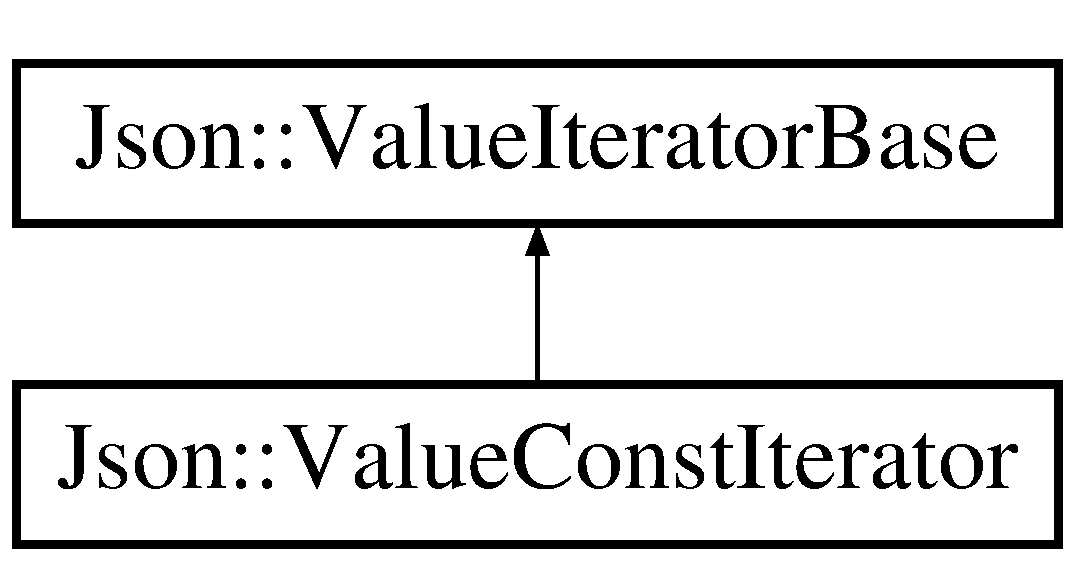
\includegraphics[height=2.000000cm]{classJson_1_1ValueConstIterator}
\end{center}
\end{figure}
\subsection*{Public Types}
\begin{DoxyCompactItemize}
\item 
\mbox{\Hypertarget{classJson_1_1ValueConstIterator_aa5f1707dcef4bfe73e23ddc14dbe760d}\label{classJson_1_1ValueConstIterator_aa5f1707dcef4bfe73e23ddc14dbe760d}} 
typedef const \hyperlink{classJson_1_1Value}{Value} {\bfseries value\+\_\+type}
\item 
\mbox{\Hypertarget{classJson_1_1ValueConstIterator_aa9b05c6a37cd352ea1ee6e13b816f709}\label{classJson_1_1ValueConstIterator_aa9b05c6a37cd352ea1ee6e13b816f709}} 
typedef const \hyperlink{classJson_1_1Value}{Value} \& {\bfseries reference}
\item 
\mbox{\Hypertarget{classJson_1_1ValueConstIterator_a400136bd8bc09e9fddec0785fa2cff14}\label{classJson_1_1ValueConstIterator_a400136bd8bc09e9fddec0785fa2cff14}} 
typedef const \hyperlink{classJson_1_1Value}{Value} $\ast$ {\bfseries pointer}
\item 
\mbox{\Hypertarget{classJson_1_1ValueConstIterator_a0c2e33e7eb5a80dd8709fb28ece83933}\label{classJson_1_1ValueConstIterator_a0c2e33e7eb5a80dd8709fb28ece83933}} 
typedef \hyperlink{classJson_1_1ValueConstIterator}{Value\+Const\+Iterator} {\bfseries Self\+Type}
\end{DoxyCompactItemize}
\subsection*{Public Member Functions}
\begin{DoxyCompactItemize}
\item 
\mbox{\Hypertarget{classJson_1_1ValueConstIterator_a7ef3df204a9ae83a0d8a3cd128e05c70}\label{classJson_1_1ValueConstIterator_a7ef3df204a9ae83a0d8a3cd128e05c70}} 
{\bfseries Value\+Const\+Iterator} (\hyperlink{classJson_1_1ValueIterator}{Value\+Iterator} const \&other)
\item 
\mbox{\Hypertarget{classJson_1_1ValueConstIterator_ad1b1c11f8d7fb22d4d3c231915f2b15b}\label{classJson_1_1ValueConstIterator_ad1b1c11f8d7fb22d4d3c231915f2b15b}} 
\hyperlink{classJson_1_1ValueIteratorBase}{Self\+Type} \& {\bfseries operator=} (const \hyperlink{classJson_1_1ValueIteratorBase}{Value\+Iterator\+Base} \&other)
\item 
\mbox{\Hypertarget{classJson_1_1ValueConstIterator_ab3f0c2edbfc8f7d60645f3d597d05e28}\label{classJson_1_1ValueConstIterator_ab3f0c2edbfc8f7d60645f3d597d05e28}} 
\hyperlink{classJson_1_1ValueIteratorBase}{Self\+Type} {\bfseries operator++} (int)
\item 
\mbox{\Hypertarget{classJson_1_1ValueConstIterator_a94935961e9331c6f7b907b05ec8df75e}\label{classJson_1_1ValueConstIterator_a94935961e9331c6f7b907b05ec8df75e}} 
\hyperlink{classJson_1_1ValueIteratorBase}{Self\+Type} {\bfseries operator-\/-\/} (int)
\item 
\mbox{\Hypertarget{classJson_1_1ValueConstIterator_a31415e44e44e56fb2bfda7e8bb784646}\label{classJson_1_1ValueConstIterator_a31415e44e44e56fb2bfda7e8bb784646}} 
\hyperlink{classJson_1_1ValueIteratorBase}{Self\+Type} \& {\bfseries operator-\/-\/} ()
\item 
\mbox{\Hypertarget{classJson_1_1ValueConstIterator_a2cfe2f7a94a688186efdafb1b181c319}\label{classJson_1_1ValueConstIterator_a2cfe2f7a94a688186efdafb1b181c319}} 
\hyperlink{classJson_1_1ValueIteratorBase}{Self\+Type} \& {\bfseries operator++} ()
\item 
\mbox{\Hypertarget{classJson_1_1ValueConstIterator_ae5612dad47a6387eef71d584fb741d0c}\label{classJson_1_1ValueConstIterator_ae5612dad47a6387eef71d584fb741d0c}} 
\hyperlink{classJson_1_1Value}{reference} {\bfseries operator$\ast$} () const
\item 
\mbox{\Hypertarget{classJson_1_1ValueConstIterator_a3c608ae53c192ee846eb265bae1cfeec}\label{classJson_1_1ValueConstIterator_a3c608ae53c192ee846eb265bae1cfeec}} 
\hyperlink{classJson_1_1Value}{pointer} {\bfseries operator-\/$>$} () const
\end{DoxyCompactItemize}
\subsection*{Friends}
\begin{DoxyCompactItemize}
\item 
\mbox{\Hypertarget{classJson_1_1ValueConstIterator_aeceedf6e1a7d48a588516ce2b1983d6f}\label{classJson_1_1ValueConstIterator_aeceedf6e1a7d48a588516ce2b1983d6f}} 
class {\bfseries Value}
\end{DoxyCompactItemize}
\subsection*{Additional Inherited Members}


\subsection{Detailed Description}
const iterator for object and array value. 



The documentation for this class was generated from the following files\+:\begin{DoxyCompactItemize}
\item 
json/json.\+h\item 
jsoncpp.\+cpp\end{DoxyCompactItemize}

\hypertarget{classJson_1_1ValueIterator}{}\section{Json\+:\+:Value\+Iterator Class Reference}
\label{classJson_1_1ValueIterator}\index{Json\+::\+Value\+Iterator@{Json\+::\+Value\+Iterator}}


Iterator for object and array value.  




{\ttfamily \#include $<$json.\+h$>$}

Inheritance diagram for Json\+:\+:Value\+Iterator\+:\begin{figure}[H]
\begin{center}
\leavevmode
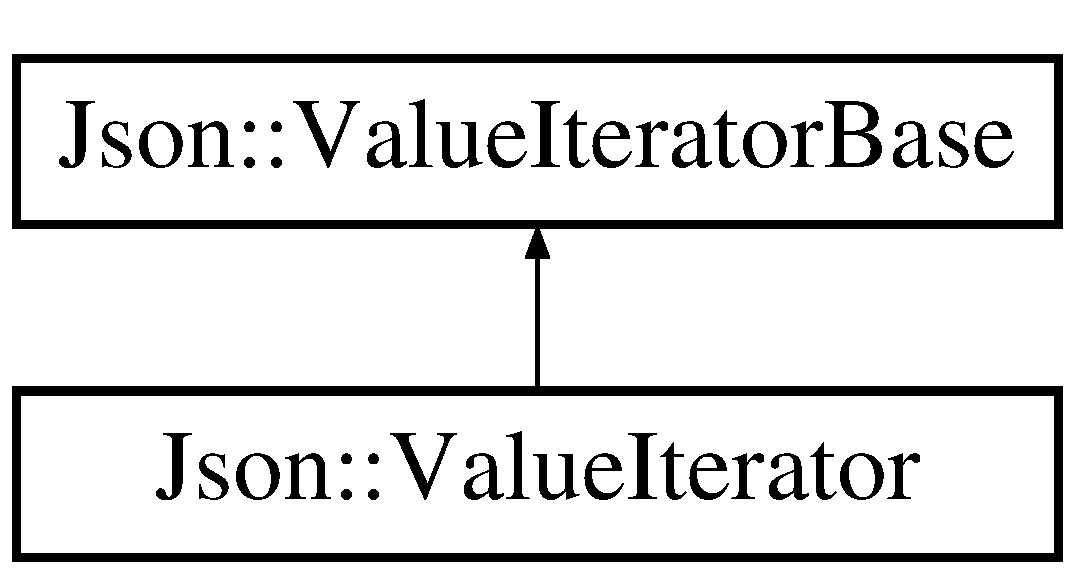
\includegraphics[height=2.000000cm]{classJson_1_1ValueIterator}
\end{center}
\end{figure}
\subsection*{Public Types}
\begin{DoxyCompactItemize}
\item 
\mbox{\Hypertarget{classJson_1_1ValueIterator_a2c5ba7be611f05546530c8a88b2d2e37}\label{classJson_1_1ValueIterator_a2c5ba7be611f05546530c8a88b2d2e37}} 
typedef \hyperlink{classJson_1_1Value}{Value} {\bfseries value\+\_\+type}
\item 
\mbox{\Hypertarget{classJson_1_1ValueIterator_a308b8932ffc83eaa9d12dadd5c11a7dd}\label{classJson_1_1ValueIterator_a308b8932ffc83eaa9d12dadd5c11a7dd}} 
typedef unsigned int {\bfseries size\+\_\+t}
\item 
\mbox{\Hypertarget{classJson_1_1ValueIterator_a2be1a9aa60bbfc8812e9dd1a7f1a8786}\label{classJson_1_1ValueIterator_a2be1a9aa60bbfc8812e9dd1a7f1a8786}} 
typedef int {\bfseries difference\+\_\+type}
\item 
\mbox{\Hypertarget{classJson_1_1ValueIterator_ae87929b4567aa00372cf602c43b57160}\label{classJson_1_1ValueIterator_ae87929b4567aa00372cf602c43b57160}} 
typedef \hyperlink{classJson_1_1Value}{Value} \& {\bfseries reference}
\item 
\mbox{\Hypertarget{classJson_1_1ValueIterator_acec45feb1ef1f3bf81240157d06d5432}\label{classJson_1_1ValueIterator_acec45feb1ef1f3bf81240157d06d5432}} 
typedef \hyperlink{classJson_1_1Value}{Value} $\ast$ {\bfseries pointer}
\item 
\mbox{\Hypertarget{classJson_1_1ValueIterator_a23357670fdad61792670d86f62db7e16}\label{classJson_1_1ValueIterator_a23357670fdad61792670d86f62db7e16}} 
typedef \hyperlink{classJson_1_1ValueIterator}{Value\+Iterator} {\bfseries Self\+Type}
\end{DoxyCompactItemize}
\subsection*{Public Member Functions}
\begin{DoxyCompactItemize}
\item 
\mbox{\Hypertarget{classJson_1_1ValueIterator_aa85aa208670891670392259efa0143bb}\label{classJson_1_1ValueIterator_aa85aa208670891670392259efa0143bb}} 
{\bfseries Value\+Iterator} (const \hyperlink{classJson_1_1ValueConstIterator}{Value\+Const\+Iterator} \&other)
\item 
\mbox{\Hypertarget{classJson_1_1ValueIterator_a7d5e58a9a4a553968acdf3064b39d21c}\label{classJson_1_1ValueIterator_a7d5e58a9a4a553968acdf3064b39d21c}} 
{\bfseries Value\+Iterator} (const \hyperlink{classJson_1_1ValueIterator}{Value\+Iterator} \&other)
\item 
\mbox{\Hypertarget{classJson_1_1ValueIterator_a8e23312b1db874f7e403fd7e76611bdc}\label{classJson_1_1ValueIterator_a8e23312b1db874f7e403fd7e76611bdc}} 
\hyperlink{classJson_1_1ValueIteratorBase}{Self\+Type} \& {\bfseries operator=} (const \hyperlink{classJson_1_1ValueIteratorBase}{Self\+Type} \&other)
\item 
\mbox{\Hypertarget{classJson_1_1ValueIterator_abcf4ddd994a010742cd4a436d65acd08}\label{classJson_1_1ValueIterator_abcf4ddd994a010742cd4a436d65acd08}} 
\hyperlink{classJson_1_1ValueIteratorBase}{Self\+Type} {\bfseries operator++} (int)
\item 
\mbox{\Hypertarget{classJson_1_1ValueIterator_a06d6a29d96caf6af324a53973159e12b}\label{classJson_1_1ValueIterator_a06d6a29d96caf6af324a53973159e12b}} 
\hyperlink{classJson_1_1ValueIteratorBase}{Self\+Type} {\bfseries operator-\/-\/} (int)
\item 
\mbox{\Hypertarget{classJson_1_1ValueIterator_a811302a868518a0995a9def955df5720}\label{classJson_1_1ValueIterator_a811302a868518a0995a9def955df5720}} 
\hyperlink{classJson_1_1ValueIteratorBase}{Self\+Type} \& {\bfseries operator-\/-\/} ()
\item 
\mbox{\Hypertarget{classJson_1_1ValueIterator_a92146c46f8249e2b2d12869e70cd4cee}\label{classJson_1_1ValueIterator_a92146c46f8249e2b2d12869e70cd4cee}} 
\hyperlink{classJson_1_1ValueIteratorBase}{Self\+Type} \& {\bfseries operator++} ()
\item 
\mbox{\Hypertarget{classJson_1_1ValueIterator_a3be48b0c1729ec2532f1ff27ad465d32}\label{classJson_1_1ValueIterator_a3be48b0c1729ec2532f1ff27ad465d32}} 
\hyperlink{classJson_1_1Value}{reference} {\bfseries operator$\ast$} () const
\item 
\mbox{\Hypertarget{classJson_1_1ValueIterator_a8dfc1603f92467591d524d0326f35534}\label{classJson_1_1ValueIterator_a8dfc1603f92467591d524d0326f35534}} 
\hyperlink{classJson_1_1Value}{pointer} {\bfseries operator-\/$>$} () const
\end{DoxyCompactItemize}
\subsection*{Friends}
\begin{DoxyCompactItemize}
\item 
\mbox{\Hypertarget{classJson_1_1ValueIterator_aeceedf6e1a7d48a588516ce2b1983d6f}\label{classJson_1_1ValueIterator_aeceedf6e1a7d48a588516ce2b1983d6f}} 
class {\bfseries Value}
\end{DoxyCompactItemize}
\subsection*{Additional Inherited Members}


\subsection{Detailed Description}
Iterator for object and array value. 

The documentation for this class was generated from the following files\+:\begin{DoxyCompactItemize}
\item 
json/json.\+h\item 
jsoncpp.\+cpp\end{DoxyCompactItemize}

\hypertarget{classJson_1_1ValueIteratorBase}{}\section{Json\+:\+:Value\+Iterator\+Base Class Reference}
\label{classJson_1_1ValueIteratorBase}\index{Json\+::\+Value\+Iterator\+Base@{Json\+::\+Value\+Iterator\+Base}}


base class for \hyperlink{classJson_1_1Value}{Value} iterators.  




{\ttfamily \#include $<$json.\+h$>$}

Inheritance diagram for Json\+:\+:Value\+Iterator\+Base\+:\begin{figure}[H]
\begin{center}
\leavevmode
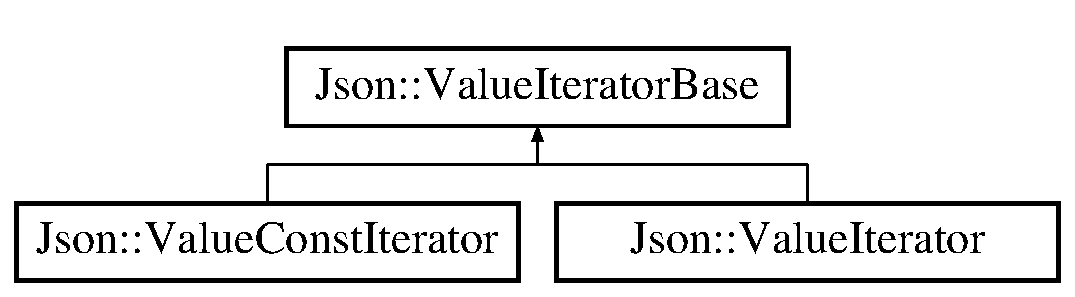
\includegraphics[height=2.000000cm]{classJson_1_1ValueIteratorBase}
\end{center}
\end{figure}
\subsection*{Public Types}
\begin{DoxyCompactItemize}
\item 
\mbox{\Hypertarget{classJson_1_1ValueIteratorBase_a02fd11a4fbdc0007da1e8bcf5e6b83c3}\label{classJson_1_1ValueIteratorBase_a02fd11a4fbdc0007da1e8bcf5e6b83c3}} 
typedef std\+::bidirectional\+\_\+iterator\+\_\+tag {\bfseries iterator\+\_\+category}
\item 
\mbox{\Hypertarget{classJson_1_1ValueIteratorBase_a9d3a3c7ce5cdefe23cb486239cf07bb5}\label{classJson_1_1ValueIteratorBase_a9d3a3c7ce5cdefe23cb486239cf07bb5}} 
typedef unsigned int {\bfseries size\+\_\+t}
\item 
\mbox{\Hypertarget{classJson_1_1ValueIteratorBase_a4e44bf8cbd17ec8d6e2c185904a15ebd}\label{classJson_1_1ValueIteratorBase_a4e44bf8cbd17ec8d6e2c185904a15ebd}} 
typedef int {\bfseries difference\+\_\+type}
\item 
\mbox{\Hypertarget{classJson_1_1ValueIteratorBase_a9d2a940d03ea06d20d972f41a89149ee}\label{classJson_1_1ValueIteratorBase_a9d2a940d03ea06d20d972f41a89149ee}} 
typedef \hyperlink{classJson_1_1ValueIteratorBase}{Value\+Iterator\+Base} {\bfseries Self\+Type}
\end{DoxyCompactItemize}
\subsection*{Public Member Functions}
\begin{DoxyCompactItemize}
\item 
\mbox{\Hypertarget{classJson_1_1ValueIteratorBase_a1248d8016f88b51371a0fcbd355b3cfd}\label{classJson_1_1ValueIteratorBase_a1248d8016f88b51371a0fcbd355b3cfd}} 
bool {\bfseries operator==} (const \hyperlink{classJson_1_1ValueIteratorBase}{Self\+Type} \&other) const
\item 
\mbox{\Hypertarget{classJson_1_1ValueIteratorBase_aa83bdcc8114b7d040eb8eb42eeed5f4a}\label{classJson_1_1ValueIteratorBase_aa83bdcc8114b7d040eb8eb42eeed5f4a}} 
bool {\bfseries operator!=} (const \hyperlink{classJson_1_1ValueIteratorBase}{Self\+Type} \&other) const
\item 
\mbox{\Hypertarget{classJson_1_1ValueIteratorBase_a98e254263fca5f1fc8fcac7bcb0260bf}\label{classJson_1_1ValueIteratorBase_a98e254263fca5f1fc8fcac7bcb0260bf}} 
difference\+\_\+type {\bfseries operator-\/} (const \hyperlink{classJson_1_1ValueIteratorBase}{Self\+Type} \&other) const
\item 
\hyperlink{classJson_1_1Value}{Value} \hyperlink{classJson_1_1ValueIteratorBase_a3838ba39c43c518cf3ed4aa6ce78ccad}{key} () const
\item 
\mbox{\Hypertarget{classJson_1_1ValueIteratorBase_a549c66a0bd20e9ae772175a5c0d2e88a}\label{classJson_1_1ValueIteratorBase_a549c66a0bd20e9ae772175a5c0d2e88a}} 
U\+Int \hyperlink{classJson_1_1ValueIteratorBase_a549c66a0bd20e9ae772175a5c0d2e88a}{index} () const
\begin{DoxyCompactList}\small\item\em Return the index of the referenced \hyperlink{classJson_1_1Value}{Value}, or -\/1 if it is not an array\+Value. \end{DoxyCompactList}\item 
J\+S\+O\+N\+C\+P\+P\+\_\+\+S\+T\+R\+I\+NG \hyperlink{classJson_1_1ValueIteratorBase_a522989403c976fdbb94da846b99418db}{name} () const
\item 
char const  $\ast$ \hyperlink{classJson_1_1ValueIteratorBase_a54765da6759fd3f1edcbfbaf308ec263}{member\+Name} () const
\item 
char const  $\ast$ \hyperlink{classJson_1_1ValueIteratorBase_a391c9cbd0edf9a447b37df00e8ce6059}{member\+Name} (char const $\ast$$\ast$end) const
\item 
\mbox{\Hypertarget{classJson_1_1ValueIteratorBase_a640e990e5f03a96fd650122a2906f59d}\label{classJson_1_1ValueIteratorBase_a640e990e5f03a96fd650122a2906f59d}} 
{\bfseries Value\+Iterator\+Base} (const Value\+::\+Object\+Values\+::iterator \&current)
\end{DoxyCompactItemize}
\subsection*{Protected Member Functions}
\begin{DoxyCompactItemize}
\item 
\mbox{\Hypertarget{classJson_1_1ValueIteratorBase_aa5b75c9514a30ba2ea3c9a35c165c18e}\label{classJson_1_1ValueIteratorBase_aa5b75c9514a30ba2ea3c9a35c165c18e}} 
\hyperlink{classJson_1_1Value}{Value} \& {\bfseries deref} () const
\item 
\mbox{\Hypertarget{classJson_1_1ValueIteratorBase_afe58f9534e1fd2033419fd9fe244551e}\label{classJson_1_1ValueIteratorBase_afe58f9534e1fd2033419fd9fe244551e}} 
void {\bfseries increment} ()
\item 
\mbox{\Hypertarget{classJson_1_1ValueIteratorBase_affc8cf5ff54a9f432cc693362c153fa6}\label{classJson_1_1ValueIteratorBase_affc8cf5ff54a9f432cc693362c153fa6}} 
void {\bfseries decrement} ()
\item 
\mbox{\Hypertarget{classJson_1_1ValueIteratorBase_af11473c9e20d07782e42b52a2f9e4540}\label{classJson_1_1ValueIteratorBase_af11473c9e20d07782e42b52a2f9e4540}} 
difference\+\_\+type {\bfseries compute\+Distance} (const \hyperlink{classJson_1_1ValueIteratorBase}{Self\+Type} \&other) const
\item 
\mbox{\Hypertarget{classJson_1_1ValueIteratorBase_a010b5ad3f3337ae3732e5d7e16ca5e25}\label{classJson_1_1ValueIteratorBase_a010b5ad3f3337ae3732e5d7e16ca5e25}} 
bool {\bfseries is\+Equal} (const \hyperlink{classJson_1_1ValueIteratorBase}{Self\+Type} \&other) const
\item 
\mbox{\Hypertarget{classJson_1_1ValueIteratorBase_a496e6aba44808433ec5858c178be5719}\label{classJson_1_1ValueIteratorBase_a496e6aba44808433ec5858c178be5719}} 
void {\bfseries copy} (const \hyperlink{classJson_1_1ValueIteratorBase}{Self\+Type} \&other)
\end{DoxyCompactItemize}


\subsection{Detailed Description}
base class for \hyperlink{classJson_1_1Value}{Value} iterators. 



\subsection{Member Function Documentation}
\mbox{\Hypertarget{classJson_1_1ValueIteratorBase_a3838ba39c43c518cf3ed4aa6ce78ccad}\label{classJson_1_1ValueIteratorBase_a3838ba39c43c518cf3ed4aa6ce78ccad}} 
\index{Json\+::\+Value\+Iterator\+Base@{Json\+::\+Value\+Iterator\+Base}!key@{key}}
\index{key@{key}!Json\+::\+Value\+Iterator\+Base@{Json\+::\+Value\+Iterator\+Base}}
\subsubsection{\texorpdfstring{key()}{key()}}
{\footnotesize\ttfamily \hyperlink{classJson_1_1Value}{Value} Json\+::\+Value\+Iterator\+Base\+::key (\begin{DoxyParamCaption}{ }\end{DoxyParamCaption}) const}

Return either the index or the member name of the referenced value as a \hyperlink{classJson_1_1Value}{Value}. \mbox{\Hypertarget{classJson_1_1ValueIteratorBase_a54765da6759fd3f1edcbfbaf308ec263}\label{classJson_1_1ValueIteratorBase_a54765da6759fd3f1edcbfbaf308ec263}} 
\index{Json\+::\+Value\+Iterator\+Base@{Json\+::\+Value\+Iterator\+Base}!member\+Name@{member\+Name}}
\index{member\+Name@{member\+Name}!Json\+::\+Value\+Iterator\+Base@{Json\+::\+Value\+Iterator\+Base}}
\subsubsection{\texorpdfstring{member\+Name()}{memberName()}\hspace{0.1cm}{\footnotesize\ttfamily [1/2]}}
{\footnotesize\ttfamily char const  $\ast$ Json\+::\+Value\+Iterator\+Base\+::member\+Name (\begin{DoxyParamCaption}{ }\end{DoxyParamCaption}) const}

Return the member name of the referenced \hyperlink{classJson_1_1Value}{Value}. \char`\"{}\char`\"{} if it is not an object\+Value. \begin{DoxyRefDesc}{Deprecated}
\item[\hyperlink{deprecated__deprecated000004}{Deprecated}]This cannot be used for U\+T\+F-\/8 strings, since there can be embedded nulls. \end{DoxyRefDesc}
\mbox{\Hypertarget{classJson_1_1ValueIteratorBase_a391c9cbd0edf9a447b37df00e8ce6059}\label{classJson_1_1ValueIteratorBase_a391c9cbd0edf9a447b37df00e8ce6059}} 
\index{Json\+::\+Value\+Iterator\+Base@{Json\+::\+Value\+Iterator\+Base}!member\+Name@{member\+Name}}
\index{member\+Name@{member\+Name}!Json\+::\+Value\+Iterator\+Base@{Json\+::\+Value\+Iterator\+Base}}
\subsubsection{\texorpdfstring{member\+Name()}{memberName()}\hspace{0.1cm}{\footnotesize\ttfamily [2/2]}}
{\footnotesize\ttfamily char const  $\ast$ Json\+::\+Value\+Iterator\+Base\+::member\+Name (\begin{DoxyParamCaption}\item[{char const $\ast$$\ast$}]{end }\end{DoxyParamCaption}) const}

Return the member name of the referenced \hyperlink{classJson_1_1Value}{Value}, or N\+U\+LL if it is not an object\+Value. \begin{DoxyNote}{Note}
Better version than \hyperlink{classJson_1_1ValueIteratorBase_a54765da6759fd3f1edcbfbaf308ec263}{member\+Name()}. Allows embedded nulls. 
\end{DoxyNote}
\mbox{\Hypertarget{classJson_1_1ValueIteratorBase_a522989403c976fdbb94da846b99418db}\label{classJson_1_1ValueIteratorBase_a522989403c976fdbb94da846b99418db}} 
\index{Json\+::\+Value\+Iterator\+Base@{Json\+::\+Value\+Iterator\+Base}!name@{name}}
\index{name@{name}!Json\+::\+Value\+Iterator\+Base@{Json\+::\+Value\+Iterator\+Base}}
\subsubsection{\texorpdfstring{name()}{name()}}
{\footnotesize\ttfamily J\+S\+O\+N\+C\+P\+P\+\_\+\+S\+T\+R\+I\+NG Json\+::\+Value\+Iterator\+Base\+::name (\begin{DoxyParamCaption}{ }\end{DoxyParamCaption}) const}

Return the member name of the referenced \hyperlink{classJson_1_1Value}{Value}, or \char`\"{}\char`\"{} if it is not an object\+Value. \begin{DoxyNote}{Note}
Avoid {\ttfamily c\+\_\+str()} on result, as embedded zeroes are possible. 
\end{DoxyNote}


The documentation for this class was generated from the following files\+:\begin{DoxyCompactItemize}
\item 
json/json.\+h\item 
jsoncpp.\+cpp\end{DoxyCompactItemize}

\hypertarget{structwebsocket__message}{}\section{websocket\+\_\+message Struct Reference}
\label{structwebsocket__message}\index{websocket\+\_\+message@{websocket\+\_\+message}}
\subsection*{Public Attributes}
\begin{DoxyCompactItemize}
\item 
\mbox{\Hypertarget{structwebsocket__message_aeb8922c34831455b764d83083ae39968}\label{structwebsocket__message_aeb8922c34831455b764d83083ae39968}} 
unsigned char $\ast$ {\bfseries data}
\item 
\mbox{\Hypertarget{structwebsocket__message_af7ae89c0cba9566b64a47d40c5ea700a}\label{structwebsocket__message_af7ae89c0cba9566b64a47d40c5ea700a}} 
size\+\_\+t {\bfseries size}
\item 
\mbox{\Hypertarget{structwebsocket__message_a72b32c83b4a065faac7ae28802a5adf1}\label{structwebsocket__message_a72b32c83b4a065faac7ae28802a5adf1}} 
unsigned char {\bfseries flags}
\end{DoxyCompactItemize}


The documentation for this struct was generated from the following file\+:\begin{DoxyCompactItemize}
\item 
mongoose.\+h\end{DoxyCompactItemize}

\hypertarget{structws__mask__ctx}{}\section{ws\+\_\+mask\+\_\+ctx Struct Reference}
\label{structws__mask__ctx}\index{ws\+\_\+mask\+\_\+ctx@{ws\+\_\+mask\+\_\+ctx}}
\subsection*{Public Attributes}
\begin{DoxyCompactItemize}
\item 
size\+\_\+t \hyperlink{structws__mask__ctx_a475d1d7c7e1ffef41e9ddd94c738dc93_a475d1d7c7e1ffef41e9ddd94c738dc93}{pos}
\item 
uint32\+\_\+t \hyperlink{structws__mask__ctx_a5d0e6527780100ef7cac724b7b7c43ca_a5d0e6527780100ef7cac724b7b7c43ca}{mask}
\end{DoxyCompactItemize}


\subsection{Member Data Documentation}
\mbox{\Hypertarget{structws__mask__ctx_a5d0e6527780100ef7cac724b7b7c43ca_a5d0e6527780100ef7cac724b7b7c43ca}\label{structws__mask__ctx_a5d0e6527780100ef7cac724b7b7c43ca_a5d0e6527780100ef7cac724b7b7c43ca}} 
\index{ws\+\_\+mask\+\_\+ctx@{ws\+\_\+mask\+\_\+ctx}!mask@{mask}}
\index{mask@{mask}!ws\+\_\+mask\+\_\+ctx@{ws\+\_\+mask\+\_\+ctx}}
\subsubsection{\texorpdfstring{mask}{mask}}
{\footnotesize\ttfamily uint32\+\_\+t ws\+\_\+mask\+\_\+ctx\+::mask}



Referenced by mg\+\_\+send\+\_\+ws\+\_\+header(), and mg\+\_\+ws\+\_\+mask\+\_\+frame().

\mbox{\Hypertarget{structws__mask__ctx_a475d1d7c7e1ffef41e9ddd94c738dc93_a475d1d7c7e1ffef41e9ddd94c738dc93}\label{structws__mask__ctx_a475d1d7c7e1ffef41e9ddd94c738dc93_a475d1d7c7e1ffef41e9ddd94c738dc93}} 
\index{ws\+\_\+mask\+\_\+ctx@{ws\+\_\+mask\+\_\+ctx}!pos@{pos}}
\index{pos@{pos}!ws\+\_\+mask\+\_\+ctx@{ws\+\_\+mask\+\_\+ctx}}
\subsubsection{\texorpdfstring{pos}{pos}}
{\footnotesize\ttfamily size\+\_\+t ws\+\_\+mask\+\_\+ctx\+::pos}



Referenced by mg\+\_\+send\+\_\+ws\+\_\+header(), and mg\+\_\+ws\+\_\+mask\+\_\+frame().



The documentation for this struct was generated from the following file\+:\begin{DoxyCompactItemize}
\item 
\hyperlink{mongoose_8c}{mongoose.\+c}\end{DoxyCompactItemize}

\hypertarget{classTBT_1_1WSClientInterface}{}\section{T\+BT\+:\+:W\+S\+Client\+Interface Class Reference}
\label{classTBT_1_1WSClientInterface}\index{T\+B\+T\+::\+W\+S\+Client\+Interface@{T\+B\+T\+::\+W\+S\+Client\+Interface}}
Inheritance diagram for T\+BT\+:\+:W\+S\+Client\+Interface\+:\begin{figure}[H]
\begin{center}
\leavevmode
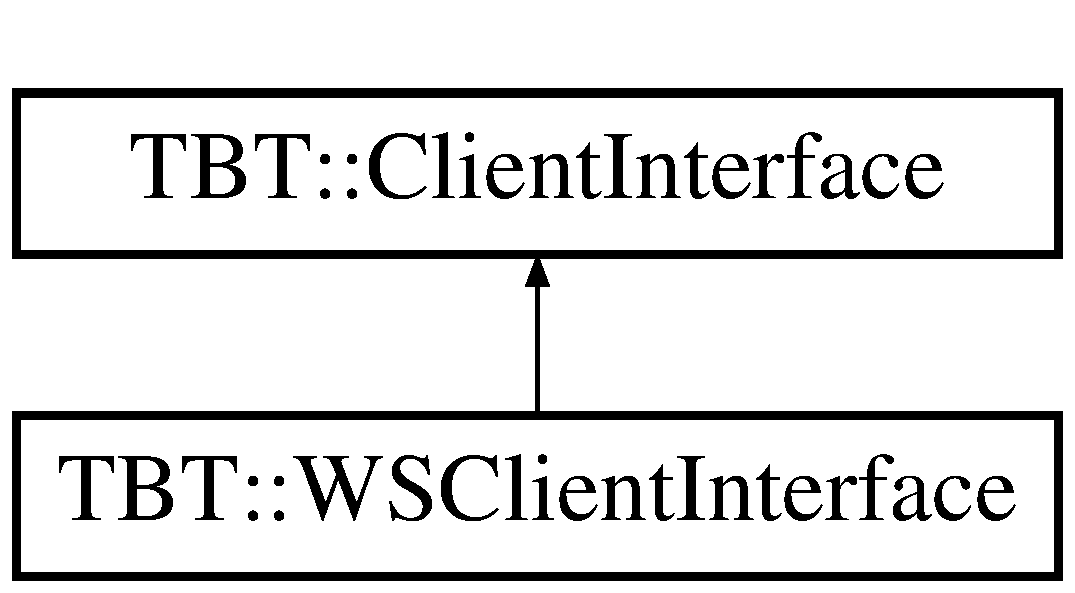
\includegraphics[height=2.000000cm]{classTBT_1_1WSClientInterface}
\end{center}
\end{figure}
\subsection*{Public Member Functions}
\begin{DoxyCompactItemize}
\item 
\mbox{\Hypertarget{classTBT_1_1WSClientInterface_addd44890c3c54a9700a2385a63105e38}\label{classTBT_1_1WSClientInterface_addd44890c3c54a9700a2385a63105e38}} 
{\bfseries W\+S\+Client\+Interface} (\hyperlink{classTBT_1_1Manager}{Manager} $\ast$p\+Manager, const char $\ast$port=W\+S\+\_\+\+P\+O\+RT)
\item 
\mbox{\Hypertarget{classTBT_1_1WSClientInterface_ad5ff4048859e3bf2fe8c62b9b2c59080}\label{classTBT_1_1WSClientInterface_ad5ff4048859e3bf2fe8c62b9b2c59080}} 
virtual void {\bfseries broadcast\+Power\+State\+Change} (Power\+State new\+State)
\item 
\mbox{\Hypertarget{classTBT_1_1WSClientInterface_a39806206461815c06c517b66d122b4db}\label{classTBT_1_1WSClientInterface_a39806206461815c06c517b66d122b4db}} 
virtual void {\bfseries broadcast\+Loc\+Info\+Change} (\hyperlink{classTBT_1_1LocDecoder}{Loc\+Decoder} $\ast$p\+Loc)
\item 
\mbox{\Hypertarget{classTBT_1_1WSClientInterface_a328ee22796e058e0da825e5f13349e1f}\label{classTBT_1_1WSClientInterface_a328ee22796e058e0da825e5f13349e1f}} 
virtual void {\bfseries broadcast\+Emergency\+Stop} (bool stop)
\end{DoxyCompactItemize}
\subsection*{Protected Attributes}
\begin{DoxyCompactItemize}
\item 
\mbox{\Hypertarget{classTBT_1_1WSClientInterface_a5a2b51f344e17b5f3e9b1f3e861b6efe}\label{classTBT_1_1WSClientInterface_a5a2b51f344e17b5f3e9b1f3e861b6efe}} 
char $\ast$ {\bfseries m\+\_\+port}
\item 
\mbox{\Hypertarget{classTBT_1_1WSClientInterface_a888e4be88a311199a3fa890d3abc6a10}\label{classTBT_1_1WSClientInterface_a888e4be88a311199a3fa890d3abc6a10}} 
volatile bool {\bfseries m\+\_\+b\+Continue}
\item 
\mbox{\Hypertarget{classTBT_1_1WSClientInterface_af8db3d6b3e3923b0b61f43cbc2021a92}\label{classTBT_1_1WSClientInterface_af8db3d6b3e3923b0b61f43cbc2021a92}} 
thread {\bfseries m\+\_\+thread}
\item 
\mbox{\Hypertarget{classTBT_1_1WSClientInterface_aba2e99d7dcc90848ce6348ee687affbb}\label{classTBT_1_1WSClientInterface_aba2e99d7dcc90848ce6348ee687affbb}} 
\hyperlink{structmg__mgr}{mg\+\_\+mgr} {\bfseries m\+\_\+mgr}
\item 
\mbox{\Hypertarget{classTBT_1_1WSClientInterface_ae866ad6fbf964a4b6ad1e19895bb24be}\label{classTBT_1_1WSClientInterface_ae866ad6fbf964a4b6ad1e19895bb24be}} 
\hyperlink{structmg__connection}{mg\+\_\+connection} $\ast$ {\bfseries m\+\_\+conn}
\end{DoxyCompactItemize}


The documentation for this class was generated from the following files\+:\begin{DoxyCompactItemize}
\item 
W\+S\+Client\+Interface.\+h\item 
W\+S\+Client\+Interface.\+cpp\end{DoxyCompactItemize}

\hypertarget{classTBT_1_1XpressNetClient}{}\section{T\+BT\+:\+:Xpress\+Net\+Client Class Reference}
\label{classTBT_1_1XpressNetClient}\index{T\+B\+T\+::\+Xpress\+Net\+Client@{T\+B\+T\+::\+Xpress\+Net\+Client}}


{\ttfamily \#include $<$Xpress\+Net\+Client.\+h$>$}

Inheritance diagram for T\+BT\+:\+:Xpress\+Net\+Client\+:\begin{figure}[H]
\begin{center}
\leavevmode
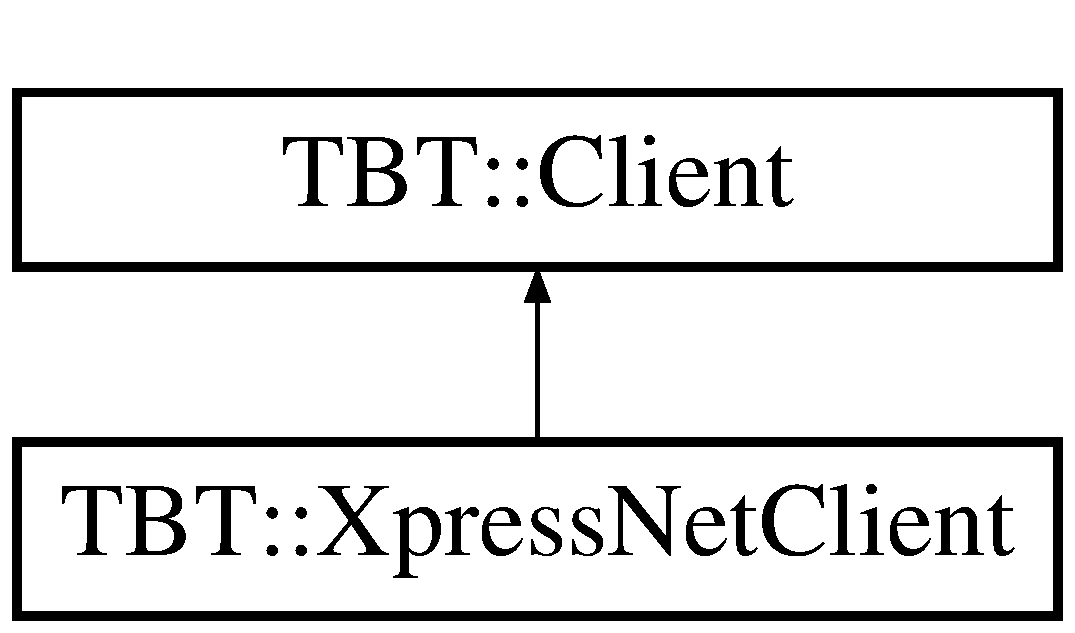
\includegraphics[height=2.000000cm]{classTBT_1_1XpressNetClient}
\end{center}
\end{figure}
\subsection*{Public Member Functions}
\begin{DoxyCompactItemize}
\item 
\hyperlink{classTBT_1_1XpressNetClient_a7647a4b5b68c29a2ed7d8832b6d1b692_a7647a4b5b68c29a2ed7d8832b6d1b692}{Xpress\+Net\+Client} (\hyperlink{classTBT_1_1ClientInterface}{Client\+Interface} $\ast$p\+Interface, uint8\+\_\+t Xpress\+Net\+Address)
\item 
virtual \hyperlink{classTBT_1_1XpressNetClient_a6c8fe1f6815ddbf26141d3ed7cdb072c_a6c8fe1f6815ddbf26141d3ed7cdb072c}{$\sim$\+Xpress\+Net\+Client} ()
\item 
const uint8\+\_\+t \& \hyperlink{classTBT_1_1XpressNetClient_aae838c0fdb74c9c7220056e3fa011390_aae838c0fdb74c9c7220056e3fa011390}{get\+Address} (void)
\item 
virtual void \hyperlink{classTBT_1_1XpressNetClient_a6f104050aad16ef336a6b83d2c60550a_a6f104050aad16ef336a6b83d2c60550a}{broadcast\+Power\+State\+Change} (bool new\+State)
\item 
virtual void \hyperlink{classTBT_1_1XpressNetClient_a0ef986da287d7fbfea163ae6016a7154_a0ef986da287d7fbfea163ae6016a7154}{broadcast\+Loc\+Info\+Changed} (\hyperlink{classTBT_1_1LocDecoder}{Loc\+Decoder} $\ast$p\+Loc)
\item 
virtual void \hyperlink{classTBT_1_1XpressNetClient_a5909e439836c772127bc24918aa0a291_a5909e439836c772127bc24918aa0a291}{broadcast\+Emergency\+Stop} (void)
\end{DoxyCompactItemize}
\subsection*{Protected Attributes}
\begin{DoxyCompactItemize}
\item 
uint8\+\_\+t \hyperlink{classTBT_1_1XpressNetClient_a9af9cd4bed2191d7504b8ae480182643_a9af9cd4bed2191d7504b8ae480182643}{m\+\_\+\+Xpress\+Net\+Address}
\end{DoxyCompactItemize}


\subsection{Constructor \& Destructor Documentation}
\mbox{\Hypertarget{classTBT_1_1XpressNetClient_a7647a4b5b68c29a2ed7d8832b6d1b692_a7647a4b5b68c29a2ed7d8832b6d1b692}\label{classTBT_1_1XpressNetClient_a7647a4b5b68c29a2ed7d8832b6d1b692_a7647a4b5b68c29a2ed7d8832b6d1b692}} 
\index{T\+B\+T\+::\+Xpress\+Net\+Client@{T\+B\+T\+::\+Xpress\+Net\+Client}!Xpress\+Net\+Client@{Xpress\+Net\+Client}}
\index{Xpress\+Net\+Client@{Xpress\+Net\+Client}!T\+B\+T\+::\+Xpress\+Net\+Client@{T\+B\+T\+::\+Xpress\+Net\+Client}}
\subsubsection{\texorpdfstring{Xpress\+Net\+Client()}{XpressNetClient()}}
{\footnotesize\ttfamily T\+B\+T\+::\+Xpress\+Net\+Client\+::\+Xpress\+Net\+Client (\begin{DoxyParamCaption}\item[{\hyperlink{classTBT_1_1ClientInterface}{Client\+Interface} $\ast$}]{p\+Interface,  }\item[{uint8\+\_\+t}]{Xpress\+Net\+Address }\end{DoxyParamCaption})}

\mbox{\Hypertarget{classTBT_1_1XpressNetClient_a6c8fe1f6815ddbf26141d3ed7cdb072c_a6c8fe1f6815ddbf26141d3ed7cdb072c}\label{classTBT_1_1XpressNetClient_a6c8fe1f6815ddbf26141d3ed7cdb072c_a6c8fe1f6815ddbf26141d3ed7cdb072c}} 
\index{T\+B\+T\+::\+Xpress\+Net\+Client@{T\+B\+T\+::\+Xpress\+Net\+Client}!````~Xpress\+Net\+Client@{$\sim$\+Xpress\+Net\+Client}}
\index{````~Xpress\+Net\+Client@{$\sim$\+Xpress\+Net\+Client}!T\+B\+T\+::\+Xpress\+Net\+Client@{T\+B\+T\+::\+Xpress\+Net\+Client}}
\subsubsection{\texorpdfstring{$\sim$\+Xpress\+Net\+Client()}{~XpressNetClient()}}
{\footnotesize\ttfamily T\+B\+T\+::\+Xpress\+Net\+Client\+::$\sim$\+Xpress\+Net\+Client (\begin{DoxyParamCaption}{ }\end{DoxyParamCaption})\hspace{0.3cm}{\ttfamily [virtual]}}



\subsection{Member Function Documentation}
\mbox{\Hypertarget{classTBT_1_1XpressNetClient_a5909e439836c772127bc24918aa0a291_a5909e439836c772127bc24918aa0a291}\label{classTBT_1_1XpressNetClient_a5909e439836c772127bc24918aa0a291_a5909e439836c772127bc24918aa0a291}} 
\index{T\+B\+T\+::\+Xpress\+Net\+Client@{T\+B\+T\+::\+Xpress\+Net\+Client}!broadcast\+Emergency\+Stop@{broadcast\+Emergency\+Stop}}
\index{broadcast\+Emergency\+Stop@{broadcast\+Emergency\+Stop}!T\+B\+T\+::\+Xpress\+Net\+Client@{T\+B\+T\+::\+Xpress\+Net\+Client}}
\subsubsection{\texorpdfstring{broadcast\+Emergency\+Stop()}{broadcastEmergencyStop()}}
{\footnotesize\ttfamily virtual void T\+B\+T\+::\+Xpress\+Net\+Client\+::broadcast\+Emergency\+Stop (\begin{DoxyParamCaption}\item[{void}]{ }\end{DoxyParamCaption})\hspace{0.3cm}{\ttfamily [inline]}, {\ttfamily [virtual]}}



Implements \hyperlink{classTBT_1_1Client_a59459df809a663bcbbb6d31fbfa09402_a59459df809a663bcbbb6d31fbfa09402}{T\+B\+T\+::\+Client}.

\mbox{\Hypertarget{classTBT_1_1XpressNetClient_a0ef986da287d7fbfea163ae6016a7154_a0ef986da287d7fbfea163ae6016a7154}\label{classTBT_1_1XpressNetClient_a0ef986da287d7fbfea163ae6016a7154_a0ef986da287d7fbfea163ae6016a7154}} 
\index{T\+B\+T\+::\+Xpress\+Net\+Client@{T\+B\+T\+::\+Xpress\+Net\+Client}!broadcast\+Loc\+Info\+Changed@{broadcast\+Loc\+Info\+Changed}}
\index{broadcast\+Loc\+Info\+Changed@{broadcast\+Loc\+Info\+Changed}!T\+B\+T\+::\+Xpress\+Net\+Client@{T\+B\+T\+::\+Xpress\+Net\+Client}}
\subsubsection{\texorpdfstring{broadcast\+Loc\+Info\+Changed()}{broadcastLocInfoChanged()}}
{\footnotesize\ttfamily void T\+B\+T\+::\+Xpress\+Net\+Client\+::broadcast\+Loc\+Info\+Changed (\begin{DoxyParamCaption}\item[{\hyperlink{classTBT_1_1LocDecoder}{Loc\+Decoder} $\ast$}]{p\+Loc }\end{DoxyParamCaption})\hspace{0.3cm}{\ttfamily [virtual]}}



Implements \hyperlink{classTBT_1_1Client_aeb3b63a37edc6b95872df54a57c27a71_aeb3b63a37edc6b95872df54a57c27a71}{T\+B\+T\+::\+Client}.



Referenced by get\+Address().

\mbox{\Hypertarget{classTBT_1_1XpressNetClient_a6f104050aad16ef336a6b83d2c60550a_a6f104050aad16ef336a6b83d2c60550a}\label{classTBT_1_1XpressNetClient_a6f104050aad16ef336a6b83d2c60550a_a6f104050aad16ef336a6b83d2c60550a}} 
\index{T\+B\+T\+::\+Xpress\+Net\+Client@{T\+B\+T\+::\+Xpress\+Net\+Client}!broadcast\+Power\+State\+Change@{broadcast\+Power\+State\+Change}}
\index{broadcast\+Power\+State\+Change@{broadcast\+Power\+State\+Change}!T\+B\+T\+::\+Xpress\+Net\+Client@{T\+B\+T\+::\+Xpress\+Net\+Client}}
\subsubsection{\texorpdfstring{broadcast\+Power\+State\+Change()}{broadcastPowerStateChange()}}
{\footnotesize\ttfamily void T\+B\+T\+::\+Xpress\+Net\+Client\+::broadcast\+Power\+State\+Change (\begin{DoxyParamCaption}\item[{bool}]{new\+State }\end{DoxyParamCaption})\hspace{0.3cm}{\ttfamily [virtual]}}



Implements \hyperlink{classTBT_1_1Client_ad64588b494ec98154ea261ed4f3b3643_ad64588b494ec98154ea261ed4f3b3643}{T\+B\+T\+::\+Client}.



Referenced by get\+Address().

\mbox{\Hypertarget{classTBT_1_1XpressNetClient_aae838c0fdb74c9c7220056e3fa011390_aae838c0fdb74c9c7220056e3fa011390}\label{classTBT_1_1XpressNetClient_aae838c0fdb74c9c7220056e3fa011390_aae838c0fdb74c9c7220056e3fa011390}} 
\index{T\+B\+T\+::\+Xpress\+Net\+Client@{T\+B\+T\+::\+Xpress\+Net\+Client}!get\+Address@{get\+Address}}
\index{get\+Address@{get\+Address}!T\+B\+T\+::\+Xpress\+Net\+Client@{T\+B\+T\+::\+Xpress\+Net\+Client}}
\subsubsection{\texorpdfstring{get\+Address()}{getAddress()}}
{\footnotesize\ttfamily const uint8\+\_\+t\& T\+B\+T\+::\+Xpress\+Net\+Client\+::get\+Address (\begin{DoxyParamCaption}\item[{void}]{ }\end{DoxyParamCaption})\hspace{0.3cm}{\ttfamily [inline]}}



References broadcast\+Loc\+Info\+Changed(), broadcast\+Power\+State\+Change(), and m\+\_\+\+Xpress\+Net\+Address.



\subsection{Member Data Documentation}
\mbox{\Hypertarget{classTBT_1_1XpressNetClient_a9af9cd4bed2191d7504b8ae480182643_a9af9cd4bed2191d7504b8ae480182643}\label{classTBT_1_1XpressNetClient_a9af9cd4bed2191d7504b8ae480182643_a9af9cd4bed2191d7504b8ae480182643}} 
\index{T\+B\+T\+::\+Xpress\+Net\+Client@{T\+B\+T\+::\+Xpress\+Net\+Client}!m\+\_\+\+Xpress\+Net\+Address@{m\+\_\+\+Xpress\+Net\+Address}}
\index{m\+\_\+\+Xpress\+Net\+Address@{m\+\_\+\+Xpress\+Net\+Address}!T\+B\+T\+::\+Xpress\+Net\+Client@{T\+B\+T\+::\+Xpress\+Net\+Client}}
\subsubsection{\texorpdfstring{m\+\_\+\+Xpress\+Net\+Address}{m\_XpressNetAddress}}
{\footnotesize\ttfamily uint8\+\_\+t T\+B\+T\+::\+Xpress\+Net\+Client\+::m\+\_\+\+Xpress\+Net\+Address\hspace{0.3cm}{\ttfamily [protected]}}



Referenced by get\+Address().



The documentation for this class was generated from the following files\+:\begin{DoxyCompactItemize}
\item 
\hyperlink{XpressNetClient_8h}{Xpress\+Net\+Client.\+h}\item 
\hyperlink{XpressNetClient_8cpp}{Xpress\+Net\+Client.\+cpp}\end{DoxyCompactItemize}

\hypertarget{classTBT_1_1XpressNetClientInterface}{}\section{T\+BT\+:\+:Xpress\+Net\+Client\+Interface Class Reference}
\label{classTBT_1_1XpressNetClientInterface}\index{T\+B\+T\+::\+Xpress\+Net\+Client\+Interface@{T\+B\+T\+::\+Xpress\+Net\+Client\+Interface}}


{\ttfamily \#include $<$Xpress\+Net\+Client\+Interface.\+h$>$}

Inheritance diagram for T\+BT\+:\+:Xpress\+Net\+Client\+Interface\+:\begin{figure}[H]
\begin{center}
\leavevmode
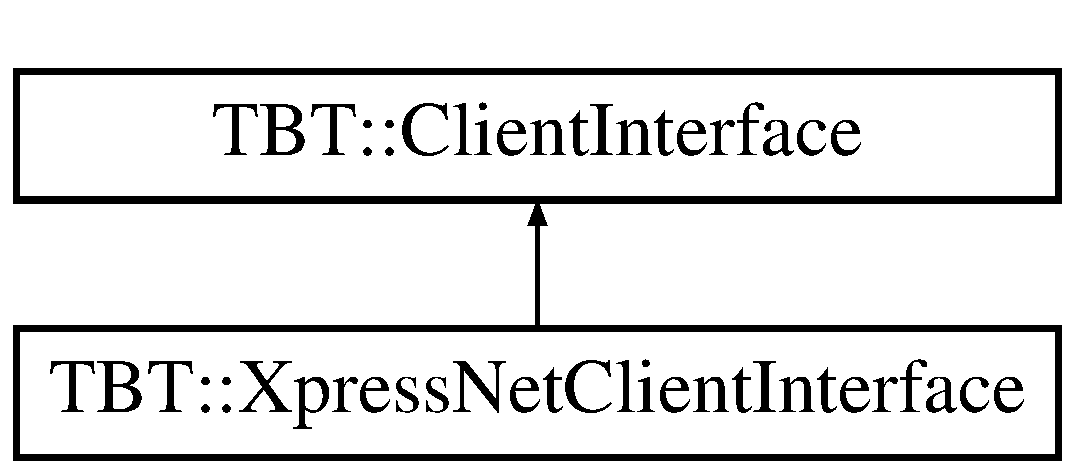
\includegraphics[height=2.000000cm]{classTBT_1_1XpressNetClientInterface}
\end{center}
\end{figure}
\subsection*{Public Member Functions}
\begin{DoxyCompactItemize}
\item 
\hyperlink{classTBT_1_1XpressNetClientInterface_afc3950ffc2b045e653c539a57967aa57_afc3950ffc2b045e653c539a57967aa57}{Xpress\+Net\+Client\+Interface} (\hyperlink{classTBT_1_1Manager}{Manager} $\ast$p\+Manager, const char $\ast$tty\+Path=\char`\"{}/dev/tty\+O1\char`\"{})
\item 
virtual \hyperlink{classTBT_1_1XpressNetClientInterface_a83f7c569ae4f17e8d9c06671166e635f_a83f7c569ae4f17e8d9c06671166e635f}{$\sim$\+Xpress\+Net\+Client\+Interface} ()
\item 
virtual void \hyperlink{classTBT_1_1XpressNetClientInterface_a338da1925ec68f197e87625c7497f472_a338da1925ec68f197e87625c7497f472}{broadcast\+Power\+State\+Change} (bool new\+State)
\item 
virtual void \hyperlink{classTBT_1_1XpressNetClientInterface_a8e64404cb84913c2d9290d2afb882b39_a8e64404cb84913c2d9290d2afb882b39}{broadcast\+Loc\+Info\+Change} (\hyperlink{classTBT_1_1LocDecoder}{Loc\+Decoder} $\ast$p\+Loc)
\item 
virtual void \hyperlink{classTBT_1_1XpressNetClientInterface_a143641241f4830f22ec5beb78036ce4c_a143641241f4830f22ec5beb78036ce4c}{broadcast\+Emergency\+Stop} (void)
\end{DoxyCompactItemize}
\subsection*{Protected Member Functions}
\begin{DoxyCompactItemize}
\item 
\hyperlink{classTBT_1_1XpressNetClient}{Xpress\+Net\+Client} $\ast$ \hyperlink{classTBT_1_1XpressNetClientInterface_ac7c05010e7a1cb8fe251c0154ca421d3_ac7c05010e7a1cb8fe251c0154ca421d3}{find\+Client} (const uint8\+\_\+t \&address)
\end{DoxyCompactItemize}
\subsection*{Private Member Functions}
\begin{DoxyCompactItemize}
\item 
void \hyperlink{classTBT_1_1XpressNetClientInterface_a8b49b38dfe0d208f643f7c65d380f31b_a8b49b38dfe0d208f643f7c65d380f31b}{thread\+Func} (void)
\end{DoxyCompactItemize}
\subsection*{Private Attributes}
\begin{DoxyCompactItemize}
\item 
char $\ast$ \hyperlink{classTBT_1_1XpressNetClientInterface_afce6612b04b468e20f8196a73bd16c7b_afce6612b04b468e20f8196a73bd16c7b}{m\+\_\+p\+Tty\+Path}
\item 
int \hyperlink{classTBT_1_1XpressNetClientInterface_a860a0570de71822774ab9d1ff14d459a_a860a0570de71822774ab9d1ff14d459a}{m\+\_\+fd\+Serial}
\item 
int \hyperlink{classTBT_1_1XpressNetClientInterface_a2a7be080da9167700fdaadbba29f1f8e_a2a7be080da9167700fdaadbba29f1f8e}{m\+\_\+fd\+Stop}
\item 
thread \hyperlink{classTBT_1_1XpressNetClientInterface_a7ed370b795990420b49cb201f3cb5c60_a7ed370b795990420b49cb201f3cb5c60}{m\+\_\+thread}
\item 
map$<$ uint8\+\_\+t, \hyperlink{classTBT_1_1XpressNetClient}{Xpress\+Net\+Client} $\ast$ $>$ \hyperlink{classTBT_1_1XpressNetClientInterface_ac064949432059e1c5210c56b43bb1168_ac064949432059e1c5210c56b43bb1168}{m\+\_\+\+Clients}
\item 
recursive\+\_\+mutex \hyperlink{classTBT_1_1XpressNetClientInterface_a22f7ef7cb7428cf26544df1bc336d517_a22f7ef7cb7428cf26544df1bc336d517}{m\+\_\+\+M\+Clients}
\end{DoxyCompactItemize}
\subsection*{Additional Inherited Members}


\subsection{Constructor \& Destructor Documentation}
\mbox{\Hypertarget{classTBT_1_1XpressNetClientInterface_afc3950ffc2b045e653c539a57967aa57_afc3950ffc2b045e653c539a57967aa57}\label{classTBT_1_1XpressNetClientInterface_afc3950ffc2b045e653c539a57967aa57_afc3950ffc2b045e653c539a57967aa57}} 
\index{T\+B\+T\+::\+Xpress\+Net\+Client\+Interface@{T\+B\+T\+::\+Xpress\+Net\+Client\+Interface}!Xpress\+Net\+Client\+Interface@{Xpress\+Net\+Client\+Interface}}
\index{Xpress\+Net\+Client\+Interface@{Xpress\+Net\+Client\+Interface}!T\+B\+T\+::\+Xpress\+Net\+Client\+Interface@{T\+B\+T\+::\+Xpress\+Net\+Client\+Interface}}
\subsubsection{\texorpdfstring{Xpress\+Net\+Client\+Interface()}{XpressNetClientInterface()}}
{\footnotesize\ttfamily T\+B\+T\+::\+Xpress\+Net\+Client\+Interface\+::\+Xpress\+Net\+Client\+Interface (\begin{DoxyParamCaption}\item[{\hyperlink{classTBT_1_1Manager}{Manager} $\ast$}]{p\+Manager,  }\item[{const char $\ast$}]{tty\+Path = {\ttfamily \char`\"{}/dev/ttyO1\char`\"{}} }\end{DoxyParamCaption})}



References m\+\_\+fd\+Serial, m\+\_\+fd\+Stop, m\+\_\+p\+Tty\+Path, m\+\_\+thread, and thread\+Func().

\mbox{\Hypertarget{classTBT_1_1XpressNetClientInterface_a83f7c569ae4f17e8d9c06671166e635f_a83f7c569ae4f17e8d9c06671166e635f}\label{classTBT_1_1XpressNetClientInterface_a83f7c569ae4f17e8d9c06671166e635f_a83f7c569ae4f17e8d9c06671166e635f}} 
\index{T\+B\+T\+::\+Xpress\+Net\+Client\+Interface@{T\+B\+T\+::\+Xpress\+Net\+Client\+Interface}!````~Xpress\+Net\+Client\+Interface@{$\sim$\+Xpress\+Net\+Client\+Interface}}
\index{````~Xpress\+Net\+Client\+Interface@{$\sim$\+Xpress\+Net\+Client\+Interface}!T\+B\+T\+::\+Xpress\+Net\+Client\+Interface@{T\+B\+T\+::\+Xpress\+Net\+Client\+Interface}}
\subsubsection{\texorpdfstring{$\sim$\+Xpress\+Net\+Client\+Interface()}{~XpressNetClientInterface()}}
{\footnotesize\ttfamily T\+B\+T\+::\+Xpress\+Net\+Client\+Interface\+::$\sim$\+Xpress\+Net\+Client\+Interface (\begin{DoxyParamCaption}{ }\end{DoxyParamCaption})\hspace{0.3cm}{\ttfamily [virtual]}}



References m\+\_\+fd\+Serial, m\+\_\+fd\+Stop, m\+\_\+p\+Tty\+Path, and m\+\_\+thread.



\subsection{Member Function Documentation}
\mbox{\Hypertarget{classTBT_1_1XpressNetClientInterface_a143641241f4830f22ec5beb78036ce4c_a143641241f4830f22ec5beb78036ce4c}\label{classTBT_1_1XpressNetClientInterface_a143641241f4830f22ec5beb78036ce4c_a143641241f4830f22ec5beb78036ce4c}} 
\index{T\+B\+T\+::\+Xpress\+Net\+Client\+Interface@{T\+B\+T\+::\+Xpress\+Net\+Client\+Interface}!broadcast\+Emergency\+Stop@{broadcast\+Emergency\+Stop}}
\index{broadcast\+Emergency\+Stop@{broadcast\+Emergency\+Stop}!T\+B\+T\+::\+Xpress\+Net\+Client\+Interface@{T\+B\+T\+::\+Xpress\+Net\+Client\+Interface}}
\subsubsection{\texorpdfstring{broadcast\+Emergency\+Stop()}{broadcastEmergencyStop()}}
{\footnotesize\ttfamily void T\+B\+T\+::\+Xpress\+Net\+Client\+Interface\+::broadcast\+Emergency\+Stop (\begin{DoxyParamCaption}\item[{void}]{ }\end{DoxyParamCaption})\hspace{0.3cm}{\ttfamily [virtual]}}



Implements \hyperlink{classTBT_1_1ClientInterface_a8d19220baccb47a7c9f45d0288bebcb8_a8d19220baccb47a7c9f45d0288bebcb8}{T\+B\+T\+::\+Client\+Interface}.



References m\+\_\+fd\+Serial.

\mbox{\Hypertarget{classTBT_1_1XpressNetClientInterface_a8e64404cb84913c2d9290d2afb882b39_a8e64404cb84913c2d9290d2afb882b39}\label{classTBT_1_1XpressNetClientInterface_a8e64404cb84913c2d9290d2afb882b39_a8e64404cb84913c2d9290d2afb882b39}} 
\index{T\+B\+T\+::\+Xpress\+Net\+Client\+Interface@{T\+B\+T\+::\+Xpress\+Net\+Client\+Interface}!broadcast\+Loc\+Info\+Change@{broadcast\+Loc\+Info\+Change}}
\index{broadcast\+Loc\+Info\+Change@{broadcast\+Loc\+Info\+Change}!T\+B\+T\+::\+Xpress\+Net\+Client\+Interface@{T\+B\+T\+::\+Xpress\+Net\+Client\+Interface}}
\subsubsection{\texorpdfstring{broadcast\+Loc\+Info\+Change()}{broadcastLocInfoChange()}}
{\footnotesize\ttfamily void T\+B\+T\+::\+Xpress\+Net\+Client\+Interface\+::broadcast\+Loc\+Info\+Change (\begin{DoxyParamCaption}\item[{\hyperlink{classTBT_1_1LocDecoder}{Loc\+Decoder} $\ast$}]{p\+Loc }\end{DoxyParamCaption})\hspace{0.3cm}{\ttfamily [virtual]}}



Implements \hyperlink{classTBT_1_1ClientInterface_aaede3709fa0dcb23743f43d9c1a5ab04_aaede3709fa0dcb23743f43d9c1a5ab04}{T\+B\+T\+::\+Client\+Interface}.

\mbox{\Hypertarget{classTBT_1_1XpressNetClientInterface_a338da1925ec68f197e87625c7497f472_a338da1925ec68f197e87625c7497f472}\label{classTBT_1_1XpressNetClientInterface_a338da1925ec68f197e87625c7497f472_a338da1925ec68f197e87625c7497f472}} 
\index{T\+B\+T\+::\+Xpress\+Net\+Client\+Interface@{T\+B\+T\+::\+Xpress\+Net\+Client\+Interface}!broadcast\+Power\+State\+Change@{broadcast\+Power\+State\+Change}}
\index{broadcast\+Power\+State\+Change@{broadcast\+Power\+State\+Change}!T\+B\+T\+::\+Xpress\+Net\+Client\+Interface@{T\+B\+T\+::\+Xpress\+Net\+Client\+Interface}}
\subsubsection{\texorpdfstring{broadcast\+Power\+State\+Change()}{broadcastPowerStateChange()}}
{\footnotesize\ttfamily void T\+B\+T\+::\+Xpress\+Net\+Client\+Interface\+::broadcast\+Power\+State\+Change (\begin{DoxyParamCaption}\item[{bool}]{new\+State }\end{DoxyParamCaption})\hspace{0.3cm}{\ttfamily [virtual]}}



Implements \hyperlink{classTBT_1_1ClientInterface_a7888a3446fb416fad75e5e008a85ca0c_a7888a3446fb416fad75e5e008a85ca0c}{T\+B\+T\+::\+Client\+Interface}.



References m\+\_\+fd\+Serial.

\mbox{\Hypertarget{classTBT_1_1XpressNetClientInterface_ac7c05010e7a1cb8fe251c0154ca421d3_ac7c05010e7a1cb8fe251c0154ca421d3}\label{classTBT_1_1XpressNetClientInterface_ac7c05010e7a1cb8fe251c0154ca421d3_ac7c05010e7a1cb8fe251c0154ca421d3}} 
\index{T\+B\+T\+::\+Xpress\+Net\+Client\+Interface@{T\+B\+T\+::\+Xpress\+Net\+Client\+Interface}!find\+Client@{find\+Client}}
\index{find\+Client@{find\+Client}!T\+B\+T\+::\+Xpress\+Net\+Client\+Interface@{T\+B\+T\+::\+Xpress\+Net\+Client\+Interface}}
\subsubsection{\texorpdfstring{find\+Client()}{findClient()}}
{\footnotesize\ttfamily \hyperlink{classTBT_1_1XpressNetClient}{Xpress\+Net\+Client} $\ast$ T\+B\+T\+::\+Xpress\+Net\+Client\+Interface\+::find\+Client (\begin{DoxyParamCaption}\item[{const uint8\+\_\+t \&}]{address }\end{DoxyParamCaption})\hspace{0.3cm}{\ttfamily [protected]}}



References m\+\_\+\+Clients, and m\+\_\+\+M\+Clients.



Referenced by thread\+Func().

\mbox{\Hypertarget{classTBT_1_1XpressNetClientInterface_a8b49b38dfe0d208f643f7c65d380f31b_a8b49b38dfe0d208f643f7c65d380f31b}\label{classTBT_1_1XpressNetClientInterface_a8b49b38dfe0d208f643f7c65d380f31b_a8b49b38dfe0d208f643f7c65d380f31b}} 
\index{T\+B\+T\+::\+Xpress\+Net\+Client\+Interface@{T\+B\+T\+::\+Xpress\+Net\+Client\+Interface}!thread\+Func@{thread\+Func}}
\index{thread\+Func@{thread\+Func}!T\+B\+T\+::\+Xpress\+Net\+Client\+Interface@{T\+B\+T\+::\+Xpress\+Net\+Client\+Interface}}
\subsubsection{\texorpdfstring{thread\+Func()}{threadFunc()}}
{\footnotesize\ttfamily void T\+B\+T\+::\+Xpress\+Net\+Client\+Interface\+::thread\+Func (\begin{DoxyParamCaption}\item[{void}]{ }\end{DoxyParamCaption})\hspace{0.3cm}{\ttfamily [private]}}



References find\+Client(), T\+B\+T\+::\+Manager\+::find\+Decoder(), T\+B\+T\+::\+Manager\+::get\+Central\+State(), T\+B\+T\+::\+Client\+::get\+Interface(), T\+B\+T\+::\+Client\+Interface\+::get\+Manager(), T\+B\+T\+::\+Loc\+Decoder\+::get\+Speedsteps(), m\+\_\+fd\+Serial, m\+\_\+fd\+Stop, N\+B\+R\+X\+P\+R\+E\+S\+S\+N\+E\+T\+P\+O\+L\+L\+E\+V\+E\+N\+TS, T\+B\+T\+::\+Power\+Off, T\+B\+T\+::\+Power\+On, T\+B\+T\+::\+Manager\+::set\+Emergency\+Stop(), T\+B\+T\+::\+Loc\+Decoder\+::set\+Function\+Group1(), T\+B\+T\+::\+Loc\+Decoder\+::set\+Function\+Group2(), T\+B\+T\+::\+Loc\+Decoder\+::set\+Function\+Group3(), T\+B\+T\+::\+Loc\+Decoder\+::set\+Function\+Group4(), T\+B\+T\+::\+Loc\+Decoder\+::set\+Function\+Group5(), T\+B\+T\+::\+Loc\+Decoder\+::set\+Loco\+Drive128(), T\+B\+T\+::\+Loc\+Decoder\+::set\+Loco\+Drive14(), T\+B\+T\+::\+Loc\+Decoder\+::set\+Loco\+Drive27(), T\+B\+T\+::\+Loc\+Decoder\+::set\+Loco\+Drive28(), and T\+B\+T\+::\+Manager\+::set\+Power\+State().



Referenced by Xpress\+Net\+Client\+Interface().



\subsection{Member Data Documentation}
\mbox{\Hypertarget{classTBT_1_1XpressNetClientInterface_ac064949432059e1c5210c56b43bb1168_ac064949432059e1c5210c56b43bb1168}\label{classTBT_1_1XpressNetClientInterface_ac064949432059e1c5210c56b43bb1168_ac064949432059e1c5210c56b43bb1168}} 
\index{T\+B\+T\+::\+Xpress\+Net\+Client\+Interface@{T\+B\+T\+::\+Xpress\+Net\+Client\+Interface}!m\+\_\+\+Clients@{m\+\_\+\+Clients}}
\index{m\+\_\+\+Clients@{m\+\_\+\+Clients}!T\+B\+T\+::\+Xpress\+Net\+Client\+Interface@{T\+B\+T\+::\+Xpress\+Net\+Client\+Interface}}
\subsubsection{\texorpdfstring{m\+\_\+\+Clients}{m\_Clients}}
{\footnotesize\ttfamily map$<$uint8\+\_\+t, \hyperlink{classTBT_1_1XpressNetClient}{Xpress\+Net\+Client}$\ast$$>$ T\+B\+T\+::\+Xpress\+Net\+Client\+Interface\+::m\+\_\+\+Clients\hspace{0.3cm}{\ttfamily [private]}}



Referenced by find\+Client().

\mbox{\Hypertarget{classTBT_1_1XpressNetClientInterface_a860a0570de71822774ab9d1ff14d459a_a860a0570de71822774ab9d1ff14d459a}\label{classTBT_1_1XpressNetClientInterface_a860a0570de71822774ab9d1ff14d459a_a860a0570de71822774ab9d1ff14d459a}} 
\index{T\+B\+T\+::\+Xpress\+Net\+Client\+Interface@{T\+B\+T\+::\+Xpress\+Net\+Client\+Interface}!m\+\_\+fd\+Serial@{m\+\_\+fd\+Serial}}
\index{m\+\_\+fd\+Serial@{m\+\_\+fd\+Serial}!T\+B\+T\+::\+Xpress\+Net\+Client\+Interface@{T\+B\+T\+::\+Xpress\+Net\+Client\+Interface}}
\subsubsection{\texorpdfstring{m\+\_\+fd\+Serial}{m\_fdSerial}}
{\footnotesize\ttfamily int T\+B\+T\+::\+Xpress\+Net\+Client\+Interface\+::m\+\_\+fd\+Serial\hspace{0.3cm}{\ttfamily [private]}}



Referenced by broadcast\+Emergency\+Stop(), broadcast\+Power\+State\+Change(), thread\+Func(), Xpress\+Net\+Client\+Interface(), and $\sim$\+Xpress\+Net\+Client\+Interface().

\mbox{\Hypertarget{classTBT_1_1XpressNetClientInterface_a2a7be080da9167700fdaadbba29f1f8e_a2a7be080da9167700fdaadbba29f1f8e}\label{classTBT_1_1XpressNetClientInterface_a2a7be080da9167700fdaadbba29f1f8e_a2a7be080da9167700fdaadbba29f1f8e}} 
\index{T\+B\+T\+::\+Xpress\+Net\+Client\+Interface@{T\+B\+T\+::\+Xpress\+Net\+Client\+Interface}!m\+\_\+fd\+Stop@{m\+\_\+fd\+Stop}}
\index{m\+\_\+fd\+Stop@{m\+\_\+fd\+Stop}!T\+B\+T\+::\+Xpress\+Net\+Client\+Interface@{T\+B\+T\+::\+Xpress\+Net\+Client\+Interface}}
\subsubsection{\texorpdfstring{m\+\_\+fd\+Stop}{m\_fdStop}}
{\footnotesize\ttfamily int T\+B\+T\+::\+Xpress\+Net\+Client\+Interface\+::m\+\_\+fd\+Stop\hspace{0.3cm}{\ttfamily [private]}}



Referenced by thread\+Func(), Xpress\+Net\+Client\+Interface(), and $\sim$\+Xpress\+Net\+Client\+Interface().

\mbox{\Hypertarget{classTBT_1_1XpressNetClientInterface_a22f7ef7cb7428cf26544df1bc336d517_a22f7ef7cb7428cf26544df1bc336d517}\label{classTBT_1_1XpressNetClientInterface_a22f7ef7cb7428cf26544df1bc336d517_a22f7ef7cb7428cf26544df1bc336d517}} 
\index{T\+B\+T\+::\+Xpress\+Net\+Client\+Interface@{T\+B\+T\+::\+Xpress\+Net\+Client\+Interface}!m\+\_\+\+M\+Clients@{m\+\_\+\+M\+Clients}}
\index{m\+\_\+\+M\+Clients@{m\+\_\+\+M\+Clients}!T\+B\+T\+::\+Xpress\+Net\+Client\+Interface@{T\+B\+T\+::\+Xpress\+Net\+Client\+Interface}}
\subsubsection{\texorpdfstring{m\+\_\+\+M\+Clients}{m\_MClients}}
{\footnotesize\ttfamily recursive\+\_\+mutex T\+B\+T\+::\+Xpress\+Net\+Client\+Interface\+::m\+\_\+\+M\+Clients\hspace{0.3cm}{\ttfamily [private]}}



Referenced by find\+Client().

\mbox{\Hypertarget{classTBT_1_1XpressNetClientInterface_afce6612b04b468e20f8196a73bd16c7b_afce6612b04b468e20f8196a73bd16c7b}\label{classTBT_1_1XpressNetClientInterface_afce6612b04b468e20f8196a73bd16c7b_afce6612b04b468e20f8196a73bd16c7b}} 
\index{T\+B\+T\+::\+Xpress\+Net\+Client\+Interface@{T\+B\+T\+::\+Xpress\+Net\+Client\+Interface}!m\+\_\+p\+Tty\+Path@{m\+\_\+p\+Tty\+Path}}
\index{m\+\_\+p\+Tty\+Path@{m\+\_\+p\+Tty\+Path}!T\+B\+T\+::\+Xpress\+Net\+Client\+Interface@{T\+B\+T\+::\+Xpress\+Net\+Client\+Interface}}
\subsubsection{\texorpdfstring{m\+\_\+p\+Tty\+Path}{m\_pTtyPath}}
{\footnotesize\ttfamily char$\ast$ T\+B\+T\+::\+Xpress\+Net\+Client\+Interface\+::m\+\_\+p\+Tty\+Path\hspace{0.3cm}{\ttfamily [private]}}



Referenced by Xpress\+Net\+Client\+Interface(), and $\sim$\+Xpress\+Net\+Client\+Interface().

\mbox{\Hypertarget{classTBT_1_1XpressNetClientInterface_a7ed370b795990420b49cb201f3cb5c60_a7ed370b795990420b49cb201f3cb5c60}\label{classTBT_1_1XpressNetClientInterface_a7ed370b795990420b49cb201f3cb5c60_a7ed370b795990420b49cb201f3cb5c60}} 
\index{T\+B\+T\+::\+Xpress\+Net\+Client\+Interface@{T\+B\+T\+::\+Xpress\+Net\+Client\+Interface}!m\+\_\+thread@{m\+\_\+thread}}
\index{m\+\_\+thread@{m\+\_\+thread}!T\+B\+T\+::\+Xpress\+Net\+Client\+Interface@{T\+B\+T\+::\+Xpress\+Net\+Client\+Interface}}
\subsubsection{\texorpdfstring{m\+\_\+thread}{m\_thread}}
{\footnotesize\ttfamily thread T\+B\+T\+::\+Xpress\+Net\+Client\+Interface\+::m\+\_\+thread\hspace{0.3cm}{\ttfamily [private]}}



Referenced by Xpress\+Net\+Client\+Interface(), and $\sim$\+Xpress\+Net\+Client\+Interface().



The documentation for this class was generated from the following files\+:\begin{DoxyCompactItemize}
\item 
\hyperlink{XpressNetClientInterface_8h}{Xpress\+Net\+Client\+Interface.\+h}\item 
\hyperlink{XpressNetClientInterface_8cpp}{Xpress\+Net\+Client\+Interface.\+cpp}\end{DoxyCompactItemize}

%--- End generated contents ---

% Index
\backmatter
\newpage
\phantomsection
\clearemptydoublepage
\addcontentsline{toc}{chapter}{Index}
\printindex

\end{document}
